% Options for packages loaded elsewhere
% Options for packages loaded elsewhere
\PassOptionsToPackage{unicode}{hyperref}
\PassOptionsToPackage{hyphens}{url}
\PassOptionsToPackage{dvipsnames,svgnames,x11names}{xcolor}
%
\documentclass[
  letterpaper,
  DIV=11,
  numbers=noendperiod]{scrreprt}
\usepackage{xcolor}
\usepackage{amsmath,amssymb}
\setcounter{secnumdepth}{5}
\usepackage{iftex}
\ifPDFTeX
  \usepackage[T1]{fontenc}
  \usepackage[utf8]{inputenc}
  \usepackage{textcomp} % provide euro and other symbols
\else % if luatex or xetex
  \usepackage{unicode-math} % this also loads fontspec
  \defaultfontfeatures{Scale=MatchLowercase}
  \defaultfontfeatures[\rmfamily]{Ligatures=TeX,Scale=1}
\fi
\usepackage{lmodern}
\ifPDFTeX\else
  % xetex/luatex font selection
\fi
% Use upquote if available, for straight quotes in verbatim environments
\IfFileExists{upquote.sty}{\usepackage{upquote}}{}
\IfFileExists{microtype.sty}{% use microtype if available
  \usepackage[]{microtype}
  \UseMicrotypeSet[protrusion]{basicmath} % disable protrusion for tt fonts
}{}
\makeatletter
\@ifundefined{KOMAClassName}{% if non-KOMA class
  \IfFileExists{parskip.sty}{%
    \usepackage{parskip}
  }{% else
    \setlength{\parindent}{0pt}
    \setlength{\parskip}{6pt plus 2pt minus 1pt}}
}{% if KOMA class
  \KOMAoptions{parskip=half}}
\makeatother
% Make \paragraph and \subparagraph free-standing
\makeatletter
\ifx\paragraph\undefined\else
  \let\oldparagraph\paragraph
  \renewcommand{\paragraph}{
    \@ifstar
      \xxxParagraphStar
      \xxxParagraphNoStar
  }
  \newcommand{\xxxParagraphStar}[1]{\oldparagraph*{#1}\mbox{}}
  \newcommand{\xxxParagraphNoStar}[1]{\oldparagraph{#1}\mbox{}}
\fi
\ifx\subparagraph\undefined\else
  \let\oldsubparagraph\subparagraph
  \renewcommand{\subparagraph}{
    \@ifstar
      \xxxSubParagraphStar
      \xxxSubParagraphNoStar
  }
  \newcommand{\xxxSubParagraphStar}[1]{\oldsubparagraph*{#1}\mbox{}}
  \newcommand{\xxxSubParagraphNoStar}[1]{\oldsubparagraph{#1}\mbox{}}
\fi
\makeatother


\usepackage{longtable,booktabs,array}
\usepackage{calc} % for calculating minipage widths
% Correct order of tables after \paragraph or \subparagraph
\usepackage{etoolbox}
\makeatletter
\patchcmd\longtable{\par}{\if@noskipsec\mbox{}\fi\par}{}{}
\makeatother
% Allow footnotes in longtable head/foot
\IfFileExists{footnotehyper.sty}{\usepackage{footnotehyper}}{\usepackage{footnote}}
\makesavenoteenv{longtable}
\usepackage{graphicx}
\makeatletter
\newsavebox\pandoc@box
\newcommand*\pandocbounded[1]{% scales image to fit in text height/width
  \sbox\pandoc@box{#1}%
  \Gscale@div\@tempa{\textheight}{\dimexpr\ht\pandoc@box+\dp\pandoc@box\relax}%
  \Gscale@div\@tempb{\linewidth}{\wd\pandoc@box}%
  \ifdim\@tempb\p@<\@tempa\p@\let\@tempa\@tempb\fi% select the smaller of both
  \ifdim\@tempa\p@<\p@\scalebox{\@tempa}{\usebox\pandoc@box}%
  \else\usebox{\pandoc@box}%
  \fi%
}
% Set default figure placement to htbp
\def\fps@figure{htbp}
\makeatother


% definitions for citeproc citations
\NewDocumentCommand\citeproctext{}{}
\NewDocumentCommand\citeproc{mm}{%
  \begingroup\def\citeproctext{#2}\cite{#1}\endgroup}
\makeatletter
 % allow citations to break across lines
 \let\@cite@ofmt\@firstofone
 % avoid brackets around text for \cite:
 \def\@biblabel#1{}
 \def\@cite#1#2{{#1\if@tempswa , #2\fi}}
\makeatother
\newlength{\cslhangindent}
\setlength{\cslhangindent}{1.5em}
\newlength{\csllabelwidth}
\setlength{\csllabelwidth}{3em}
\newenvironment{CSLReferences}[2] % #1 hanging-indent, #2 entry-spacing
 {\begin{list}{}{%
  \setlength{\itemindent}{0pt}
  \setlength{\leftmargin}{0pt}
  \setlength{\parsep}{0pt}
  % turn on hanging indent if param 1 is 1
  \ifodd #1
   \setlength{\leftmargin}{\cslhangindent}
   \setlength{\itemindent}{-1\cslhangindent}
  \fi
  % set entry spacing
  \setlength{\itemsep}{#2\baselineskip}}}
 {\end{list}}
\usepackage{calc}
\newcommand{\CSLBlock}[1]{\hfill\break\parbox[t]{\linewidth}{\strut\ignorespaces#1\strut}}
\newcommand{\CSLLeftMargin}[1]{\parbox[t]{\csllabelwidth}{\strut#1\strut}}
\newcommand{\CSLRightInline}[1]{\parbox[t]{\linewidth - \csllabelwidth}{\strut#1\strut}}
\newcommand{\CSLIndent}[1]{\hspace{\cslhangindent}#1}



\setlength{\emergencystretch}{3em} % prevent overfull lines

\providecommand{\tightlist}{%
  \setlength{\itemsep}{0pt}\setlength{\parskip}{0pt}}



 


% For ensuring two figures are on two separate pages
\usepackage{afterpage}
% For shifting footnotes to end of chapter
\usepackage{endnotes}
\let\footnote=\endnote
% For styling footnote indenting (when using endnotes)
\makeatletter
\renewcommand{\enoteformat}{%
  \setlength{\leftskip}{0pt}%
  \setlength{\parindent}{0pt}%
  \makebox[0pt][r]{${}^{\theenmark}$~}%
}
\makeatother
% For styling quotes 
\usepackage[most]{tcolorbox}
\AtBeginEnvironment{quote}{\begin{tcolorbox}[
  enhanced,
  colback=gray!10, 
  colframe=gray,
  boxrule=0pt,
  borderline west={2pt}{0pt}{gray},
  sharp corners,
  left=10pt,
  right=10pt,
  top=5pt,
  bottom=5pt
]}
\AtEndEnvironment{quote}{\end{tcolorbox}}

\usepackage{booktabs}
\usepackage{longtable}
\usepackage{array}
\usepackage{multirow}
\usepackage{wrapfig}
\usepackage{float}
\usepackage{colortbl}
\usepackage{pdflscape}
\usepackage{tabu}
\usepackage{threeparttable}
\usepackage{threeparttablex}
\usepackage[normalem]{ulem}
\usepackage{makecell}
\usepackage{xcolor}
\KOMAoption{captions}{tableheading}
\makeatletter
\@ifpackageloaded{bookmark}{}{\usepackage{bookmark}}
\makeatother
\makeatletter
\@ifpackageloaded{caption}{}{\usepackage{caption}}
\AtBeginDocument{%
\ifdefined\contentsname
  \renewcommand*\contentsname{Table of contents}
\else
  \newcommand\contentsname{Table of contents}
\fi
\ifdefined\listfigurename
  \renewcommand*\listfigurename{List of Figures}
\else
  \newcommand\listfigurename{List of Figures}
\fi
\ifdefined\listtablename
  \renewcommand*\listtablename{List of Tables}
\else
  \newcommand\listtablename{List of Tables}
\fi
\ifdefined\figurename
  \renewcommand*\figurename{Figure}
\else
  \newcommand\figurename{Figure}
\fi
\ifdefined\tablename
  \renewcommand*\tablename{Table}
\else
  \newcommand\tablename{Table}
\fi
}
\@ifpackageloaded{float}{}{\usepackage{float}}
\floatstyle{ruled}
\@ifundefined{c@chapter}{\newfloat{codelisting}{h}{lop}}{\newfloat{codelisting}{h}{lop}[chapter]}
\floatname{codelisting}{Listing}
\newcommand*\listoflistings{\listof{codelisting}{List of Listings}}
\makeatother
\makeatletter
\makeatother
\makeatletter
\@ifpackageloaded{caption}{}{\usepackage{caption}}
\@ifpackageloaded{subcaption}{}{\usepackage{subcaption}}
\makeatother
\usepackage{bookmark}
\IfFileExists{xurl.sty}{\usepackage{xurl}}{} % add URL line breaks if available
\urlstyle{same}
\hypersetup{
  pdftitle={How Data Visualisation Works},
  pdfauthor={Paul Murrell},
  colorlinks=true,
  linkcolor={blue},
  filecolor={Maroon},
  citecolor={Blue},
  urlcolor={Blue},
  pdfcreator={LaTeX via pandoc}}


\title{How Data Visualisation Works}
\author{Paul Murrell}
\date{}
\begin{document}
\maketitle

\renewcommand*\contentsname{Table of contents}
{
\hypersetup{linkcolor=}
\setcounter{tocdepth}{2}
\tableofcontents
}

\bookmarksetup{startatroot}

\chapter*{Preface}\label{preface}
\addcontentsline{toc}{chapter}{Preface}

\markboth{Preface}{Preface}

\emph{Visualization is essentially a mapping process from computer
representations to perceptual representations, choosing encoding
techniques to maximize human understanding and
communication.}\footnote{This quote is from an early web resource on
  data visualisation that was produced by the ACM SIGGRAPH Education
  Committee (Owen et al. 1999).}

This is a book about data visualisation.

Like many books, it scratches an author's itch.

This particular itch began a long time ago, when first introduced to the
works of Edward Tufte. Books like \emph{The Visual Display of
Quantitative Information} and \emph{Envisioning Information}\footnote{\emph{The
  Visual Display of Quantitative Information} (Tufte 1983) and
  \emph{Envisioning Information} (Tufte 1990) are just two of a series
  of influential and visually attractive books that also includes
  \emph{Visual Explanations} (Tufte 1997) and \emph{Beautiful Evidence}
  (Tufte 2006).} inspired an interest in how to produce effective
graphics, but they were also frustrating.

Reading a Tufte book to get better at data visualisation is a bit like
watching Roger Federer play to get better at tennis. It is possible to
glean fragments of insight into the master's skill and technique, but it
is difficult to come away with a clear set of rules for how to succeed
on our own.

At the same time, encountering the work of William S. Cleveland
presented a different problem.\footnote{There were several studies by
  Cleveland, some in collaboration with Robert McGill, which were
  summarised and extended in two books: \emph{The Elements of Graphing
  Data} (William S. Cleveland 1985b) and \emph{Visualizing Data}
  (William S. Cleveland 1993).} Here were hard experimental results with
clear implications for effective data visualisations: use length not
area; use bars not pies. But they only told us about a small subset of
the types of data visualisations that we could create and they only told
us about a small subset of the types of questions that we could answer
with those data visualisations.

In the intervening decades since those first encounters, a lot has
happened.

Data visualisation is an area of research for psychologists, for
computer scientists, for geographers, and even for statisticians. The
literature is wide and deep and complex.

This has significantly reduced the size of the second problem. We know a
lot more about a wider range of data visualisation types and data
visualisation tasks. Unfortunately, this has introduced a new problem.
There are comprehensive and detailed overviews of current
knowledge,\footnote{\emph{Information Visualization: Perception for
  Design} (Ware 2021) reviews a very wide range of research that has
  relevance to data visualisation in one way or another and
  \emph{Visualization Analysis and Design} (Munzner 2014) provides a
  comprehensive and theoretical coverage of the complete process of
  creating effective data visualisations.} but it is now difficult to
consume and make sense of so much knowledge.

At the same time, there are more accessible and practical guides for
creating effective data visualisations.\footnote{For example,
  \emph{Creating More Effective Graphs} (Robbins 2005), \emph{Data
  Visualization: A Practical Introduction} (Healy 2018), and
  \emph{Fundamentals of Data Visualization: A Primer on Making
  Informative and Compelling Figures} (Wilke 2019).} These eschew much
of the gory detail in favour of simple, applicable advice. The problem
here is that, without the underlying explanations, the guidelines can
become just a long laundry list to commit to memory. It is useful to
know that bars should always start at zero, but is more satisfying to
know why.

For some of us there is a need for a middle path. We would like to
understand why we are making certain data visualisation choices, but we
have brains that can only hold so many ideas at once. For us there is
utility in a framework that contains a small number of core concepts,
that covers a wide range of data visualisations, but connects them all
with a relatively simple explanation.

This book attempts to provide such a framework. It is a synthesis of a
large number of research articles and books and it is a simplification
of a large amount of knowledge. It is an attempt to prune the complexity
so that we can see the forest through the trees, while at the same time
leaving enough foliage that we can still recognise a tree when we see
one.

I hope that it helps.

\section*{How to Read this Book}\label{how-to-read-this-book}
\addcontentsline{toc}{section}{How to Read this Book}

\markright{How to Read this Book}

Although the goal is to provide a relatively simple conceptual framework
for thinking about data visualisation, this is not a short book. The
\href{exec.html}{Executive Summary} provides the simplest possible
statement of the framework and it may be useful to resurface and revisit
this summary if you become lost in the depths of one of the chapters.

A slightly longer summary of the framework is provided in the
\href{review.html}{Review}. The Review also provides some guidance on
how the framework can be applied to the creation of a new data
visualisation and the criticism of existing an one.

Another major issue with a subject this complex and a subject that is
studied from so many different angles is \emph{terminology}. There is no
consistency across all of the different sources of information from
which this book was drawn, so all that we can do is attempt to be
consistent with ourselves. Some of the most important terms that will be
reused relentlessly throughout this book are highlighted in the
\href{exec.html}{Executive Summary}. The meaning of these terms is
hopefully approximately what you already think, but they will be made
clearer as the book progresses.

All section and figure cross-references are hyperlinks, so clicking them
will navigate to the relevant section or figure. Even more helpfully,
hovering the mouse over a hyperlink will show a preview of the relevant
section or figure. This is particularly effective for figures because it
obviates the need to reproduce the same image multiple times; just hover
over the figure link to see the image that the text is referring to.

\section*{Acknowledgements}\label{acknowledgements}
\addcontentsline{toc}{section}{Acknowledgements}

\markright{Acknowledgements}

This book is based upon a large number of research articles and books,
but in order to make the text appear more accessible and friendly, there
are no formal citations in the main text. There are, however, a large
number of footnotes, which provide the links between what is being
described in the main text and the underlying research, and those
footnotes contain proper citations. The real work is not being ignored,
it is just being hidden from view.

This book has been generated using the \href{https://quarto.org/}{Quarto
publishing system}. If any parts of the book look nice to you it is
probably thanks to Quarto.

\begin{center}\rule{0.5\linewidth}{0.5pt}\end{center}

\theendnotes

\bookmarksetup{startatroot}

\chapter*{Executive Summary}\label{sec-exec}
\addcontentsline{toc}{chapter}{Executive Summary}

\markboth{Executive Summary}{Executive Summary}

\begin{itemize}
\item
  Creating a data visualisation involves an {\textbf{encoding}} of
  {\textbf{data values}} as {\textbf{visual features}}.

  For example, numeric {\textbf{counts}} are {\textbf{encoded}} as the
  {\textbf{heights of bars}} to create a bar plot.
\item
  Reading a data visualisation involves a {\textbf{decoding}} of
  {\textbf{visual features}} to obtain {\textbf{data values}}.

  For example, the {\textbf{heights}} of bars in a bar plot are
  {\textbf{decoded}} to obtain {\textbf{counts}}.
\item
  The {\textbf{effectiveness}} of a data visualisation depends on the
  effectiveness of the {\textbf{decoding}}.

  For example, a bar plot is effective for comparing {\textbf{counts}}
  because the visual system is effective at comparing the
  {\textbf{heights}} of bars.
\item
  More {\textbf{complex encodings}} produce more {\textbf{complex visual
  features}}.

  For example, a scatter plot {\textbf{encodes}} {\textbf{two numeric
  variables}} as the x- and y-locations of points, which produces the
  {\textbf{position in space}} of points.
\item
  More {\textbf{complex visual features}} lead to more {\textbf{complex
  decodings}}.

  For example, the {\textbf{position in space}} of points in a scatter
  plot is {\textbf{decoded}} as the {\textbf{correlation}} between two
  numeric variables.
\item
  An {\textbf{effective data visualisation}} {\textbf{encodes}} data
  values to visual features that facilitate an effective
  {\textbf{decoding}} from visual features back to information about the
  data.
\end{itemize}

\bookmarksetup{startatroot}

\chapter{Introduction}\label{sec-intro}

A data visualisation presents data values in a visual format. In an
effective data visualisation, this allows properties of the data to be
perceived very rapidly and without conscious effort. For example,
Table~\ref{tbl-crime} shows data on the crime rate for youth offenders
in New Zealand, for the ages 14 to 16, for each year from 2011 to 2021.
With this purely text-based, tabular presentation of the data, it
requires considerable time and effort to determine any trends in the
crime rates.

\begin{longtable}[]{@{}rrrrrrrrrrrr@{}}

\caption{\label{tbl-crime}A table of the number of distinct youth
offenders, per 10,000 of popuplation, aged 14 to 16 from 2011 to 2021.
It is difficult to perceive trends in the crime rates from this purely
text-based, tabular presentation of the data.}

\tabularnewline

\toprule\noalign{}
age & 2011 & 2012 & 2013 & 2014 & 2015 & 2016 & 2017 & 2018 & 2019 &
2020 & 2021 \\
\midrule\noalign{}
\endhead
\bottomrule\noalign{}
\endlastfoot
14 & 583 & 524 & 446 & 378 & 318 & 305 & 280 & 281 & 270 & 244 & 219 \\
15 & 712 & 619 & 528 & 443 & 369 & 339 & 315 & 304 & 272 & 262 & 246 \\
16 & 810 & 723 & 615 & 482 & 426 & 365 & 328 & 334 & 314 & 302 & 257 \\

\end{longtable}

By contrast, with a simple line plot data visualisation like
Figure~\ref{fig-crime} we can perceive the trends in crime rates easily
and immediately. It is also easy to perceive more detailed properties
like the fact that the trend in crime rates for 16-year-olds is not
completely monotonic and the fact that the crime rate for 15-year-olds
(the blue line) is always greater than the crime rate for 14-year-olds
(the red line) and less than the crime rate for 16-year-olds (the green
line).

\begin{figure}

\centering{

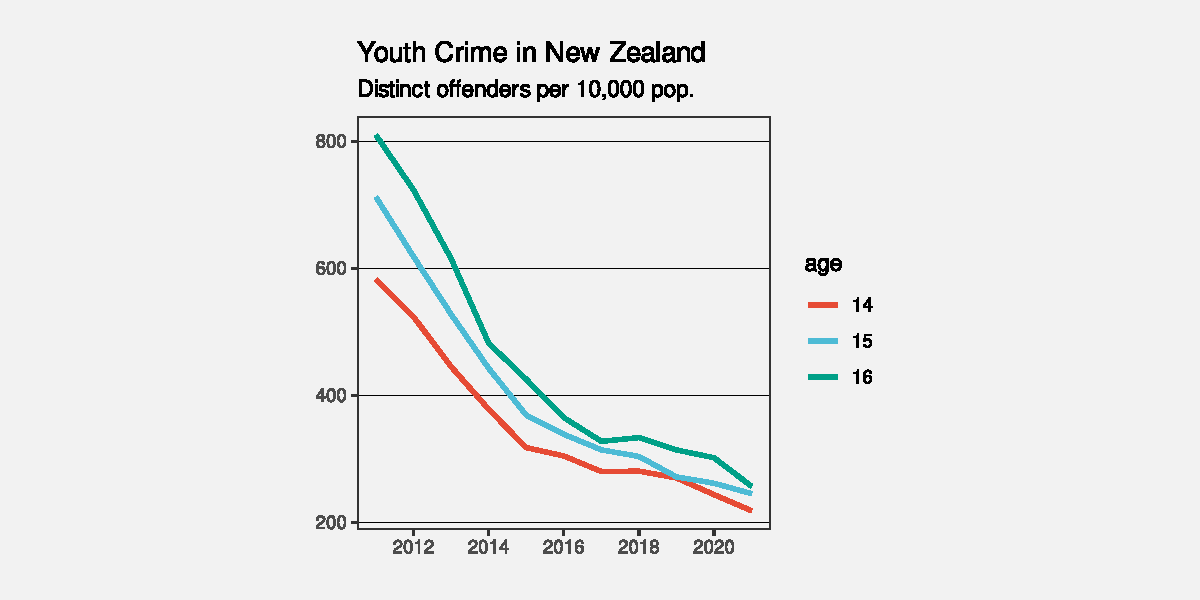
\includegraphics[width=1\linewidth,height=\textheight,keepaspectratio]{index_files/mediabag/intro_files/figure-pdf/fig-crime-1.pdf}

}

\caption{\label{fig-crime}A line plot of the crime rate amongst youth
offenders aged 14 to 16 from 2011 to 2021. Detecting trends in the crime
rates is very fast and easy with this data visualisation.}

\end{figure}%

Figure~\ref{fig-crime-heatmap} shows a different data visualisation of
the same data, this time a heatmap. If we use a data visualisation like
Figure~\ref{fig-crime-heatmap}, while very basic trends are apparent,
perceiving detailed changes in the crime rates is very much harder
compared to Figure~\ref{fig-crime}. In other words, not all data
visualisations are equally effective.

\begin{figure}

\centering{

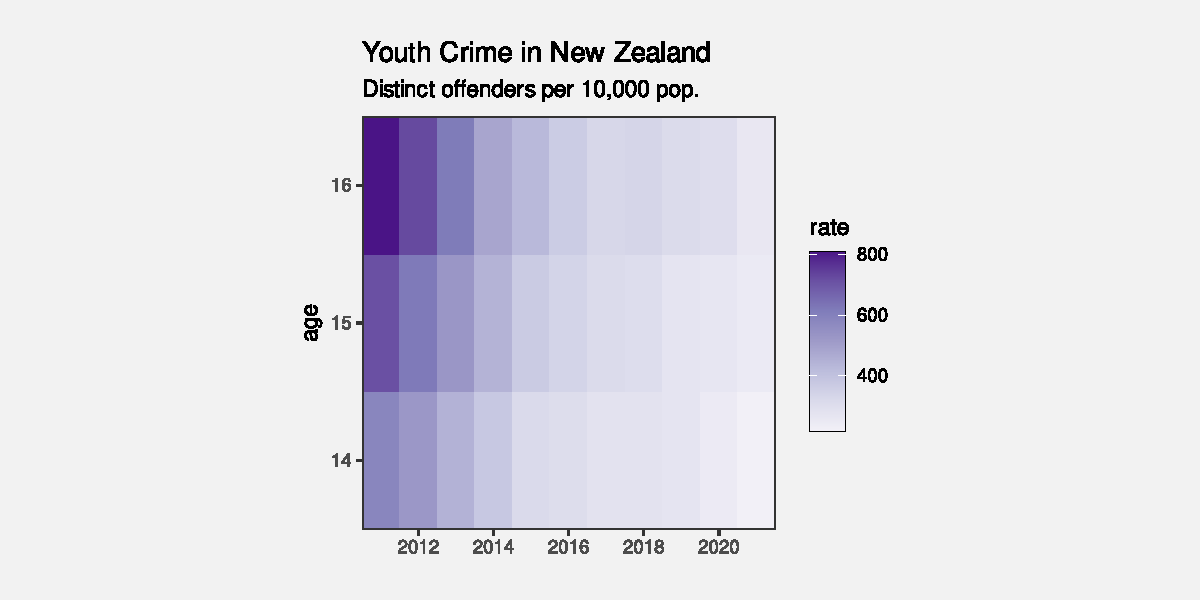
\includegraphics[width=1\linewidth,height=\textheight,keepaspectratio]{index_files/mediabag/intro_files/figure-pdf/fig-crime-heatmap-1.pdf}

}

\caption{\label{fig-crime-heatmap}A heatmap of the crime rate amongst
youth offenders aged 14 to 16 from 2011 to 2021. Some basic trends are
visible, but details are harder to perceive compared to
Figure~\ref{fig-crime}.}

\end{figure}%

Although Figure~\ref{fig-crime} is very effective for the questions that
we have considered so far, it is far less effective if we are interested
in a different question, for example, whether the \emph{total} crime
rate is completely monotonic. Does the \emph{sum} of the red, blue, and
green lines always decrease year on year? In other words, a single data
visualisation cannot be effective for all possible questions.

Suppose that we are interested in what the \emph{exact} crime rate was
for 16-year-olds in 2011. Neither Figure~\ref{fig-crime} nor
Figure~\ref{fig-crime-heatmap} is the best option for answering this
quesion. The best option in this case is actually Table~\ref{tbl-crime}.

What makes a data visualisation effective? Why are some data
visualisations more effective than others? The purpose of this book is
to provide explanations for why, when, and how data visualisation works.

\section{One big idea: Mappings}\label{sec-mappings}

Figure~\ref{fig-crime} and Figure~\ref{fig-crime-heatmap} are examples
of different types of data visualisation, a line plot and a heatmap
respectively. We will explore many different types of data
visualisations throughout the book, but rather than address each type of
data visualisation on its own, we want to identify underlying concepts
that help to explain how all data visualisations work.

One concept that we will lean on very heavily is the idea of
\textbf{mappings}: how is information being converted into a visual
representation?\footnote{The idea of characterising a data visualisation
  as a set of ``mappings'' from data values to visual representations is
  based on ideas within the \emph{Grammar of Graphics} (Wilkinson 2005).}

The most obvious mapping in a data visualisation involves the conversion
of \textbf{data values} to \textbf{data symbols}
(Figure~\ref{fig-mappings}). For example, in Figure~\ref{fig-crime}, all
of the data values for 14-year-olds, the number of offenders for each
year, have been mapped to an orange line. The data values for
15-year-olds have been mapped to a blue line and the data values for
16-year-olds have been mapped to a green line. In other words, each row
of Table~\ref{tbl-crime} is mapped to a separate coloured line.

The heatmap of the same data (see Figure~\ref{fig-crime-heatmap})
provides a different visual representation because it employs a
different mapping. In this case, the data symbol is a rectangle, with
one data symbol for each combination of age and year, and with the
colour of the rectangle reflecting the number of offenders of that age
for that year. In other words, each cell of Table~\ref{tbl-crime} is
mapped to its own coloured rectangle.

\begin{figure}

\centering{

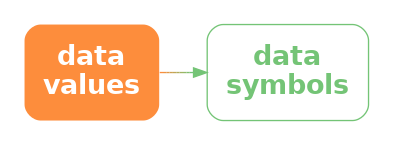
\includegraphics[scale=0.5]{Diagrams/data-sym.png}

}

\caption{\label{fig-mappings}A data visualisation can be described by
the \textbf{mappings} that it uses to represent \textbf{data values} as
\textbf{data symbols}.}

\end{figure}%

We will talk about \textbf{encoding} information using a visual
representation, for example, encoding data values as data symbols.

The journey that we take throughout this book will involve exploring a
variety of different ways that information can be mapped to a visual
representation. As much as possible, we will attempt to reduce any data
visualisation to a set of mappings from different pieces of information
to visual representations of that information. By understanding the
different mappings that we can use, we will come to understand why some
data visualisations are more effective than others.

\section{How will it help?}\label{how-will-it-help}

You may have heard that statisticians hate pie charts.\footnote{In fact,
  pie charts have received a lot of hate from all quarters for over a
  century:

  ``In a sense, it might be construed as an insult to a man's
  intelligence to show him a pie chart'' Karsten (1925, p98).

  ``the only worse design than a pie chart is several of them \ldots{}
  pie charts should never be used.'' Tufte (1983, p178).

  For some counter-arguments, see Section~\ref{sec-part-to-whole}.} But
do you know why? Do pie charts have any redeeming features?

Conversely, bar plots are extremely popular, but why are they so good?
Knowing more about why different plots work for different situations
will help us to make better decisions about when to use what sort of
data visualisation.

There is a lot of useful information and understanding about how data
visualisations work, but it is distributed throughout and embedded
within a very broad, deep, and detailed data visualisation literature.
This book aims to produce a simple, coherent explanation that is
accessible to a less expert audience.\footnote{Besides scratching the
  author's itch, this book addresses an identified need. For example,
  Sönning (2022) deconstructs how a line plot works in great detail, but
  there is a market for something that is more accessible to and
  applicable by a less-expert audience.

  ``Going forward, we must do a better job of translating the academic
  research into practice, making it easier for academics and
  nonacademics alike to create useful, well-designed graphics.''
  (Vanderplas, Cook, and Hofmann 2020)

  The aim is to provide an overview that is similar in scope to more
  expert frameworks like (Kosslyn 1989), but more consumable by a less
  expert audience. The goal of this document is to provide a description
  that is sufficiently straightforward for the non-expert to consume,
  hopefully without making too many experts roll in their graves or send
  them to an early one. In most cases, it will be easy to see for
  ourselves that a visual effect is real through a simple diagram or
  data visualisation, but references to the relevant theories and
  experimental results in the literature will be provided in footnotes
  like this one.}

Understanding how data visualisation works will enable us to:

\begin{itemize}
\tightlist
\item
  Decide which data visualisations we should use.
\item
  Justify our choice of data visualisation.
\item
  Critically analyse data visualisations created by others.
\item
  Reason about how to improve the effectiveness of a data visualisation.
\item
  Reason about whether a novel visualisation will be effective.
\end{itemize}

\section{Scope}\label{sec-scope}

The focus of this document is \textbf{static} data visualisations for
\textbf{presentation}. The assumption is that our data values have an
interesting property and we want to produce a display that makes it easy
and efficient for viewers to perceive that property. Some of the
information that we cover will also apply to interactive graphics and to
exploratory graphics, but the specific requirements of those types of
data visualisation will not be addressed.\footnote{Some examples of
  books that include a discussion of interactive graphics are Cook and
  Swayne (2007), Theus and Urbanek (2008), and Unwin, Theus, and Hofmann
  (2006).}

This document is also focused on what \textbf{vision science} has to
tell us about effective data visualisation. We will consider factors
that influence how rapidly and how accurately information can be
extracted from a data visualisation. This will include findings from a
broad range of research, encompassing Statistics, Computer Science,
Psychology, and Cartography.

However, this document does not cover all fields of research that impact
on data visualisation. We will not, for example, address the ethical use
of data visualisation, beyond a basic assumption that we want to
faithfully represent the properties of the data.\footnote{Alberto
  Cairo's writing often includes the ethical dimensions of data
  visualisation, e.g., Cairo (2014) and Cairo (2016).

  The \emph{Data by Design} project is a striking example of work with a
  focus on ethical data visualisation (Emory Digital Humanities Lab
  2021).}

This document is also aimed at a numerate audience, so we assume an
appreciation of the importance of collecting the right data in the right
way for the questions that we hope to answer.\footnote{We are assuming
  that the data we have is sufficient for the question(s) of interest
  and contains no ``substantive'' problems, in the sense of Healy
  (2018).

  Examples of books that provide a more comprehensive treatment of the
  entire data visualisation process are Cairo (2019) and Munzner (2014).

  An example of a much shorter, but still broader view of the data
  visualisation process is Bertini (2025).}

It is also important to acknowledge that vision science cannot yet tell
us everything about how data visualisation works. However, what is known
will help us to have some understanding of why some data visualisations
are so effective and others are less effective.

As well as being a synthesis of a large range of data visualisation
research, this document is also a simplification of that research. Some
details are smoothed over and some details are just left out. The goal
is to provide a framework that is easy to understand by non-experts and
easy to apply to a broad range of data visualisations. References to the
relevant literature are provided in footnotes so that the interested, or
sceptical, reader can dig deeper.

\section{Summary}\label{summary}

Data visualisations can be incredibly effective for presenting important
properties of data values. However, any one data visualisation may only
be effective for certain data values and for certain data properties.

The goal of this document is to explain why some data visualisations are
more effective than others; how data visualisation works.

We will focus on how information is \textbf{mapped} to a visual
representation. We can characterise a data visualisation in terms of the
mappings that it uses to \textbf{encode} data values as data symbols.

\begin{center}\rule{0.5\linewidth}{0.5pt}\end{center}

\theendnotes

\bookmarksetup{startatroot}

\chapter{The Visual System}\label{sec-visual-system}

Understanding why some mappings are more effective than others will
depend upon an understanding of how the human visual system works. In
particular, in order to understand the effectiveness of a mapping from
information to a visual representation, we need to know how we get from
visual representations back to the original information. In
Chapter~\ref{sec-intro}, we described a mapping as an \textbf{encoding}
of information as a visual representation. In this chapter, we will
consider the reverse operation: the \textbf{decoding} of a visual
representation back to the original information
(Figure~\ref{fig-decode}). The effectiveness of an \textbf{encoding}
from data values to data symbols will depend on how well we can
\textbf{decode} from the data symbols back to data values.

In this chapter we will establish a very simple model of the visual
system, which will help us to understand the effectiveness of the
different mappings that we consider throughout the book.\footnote{Simple
  descriptions of the human visual system can be found in many articles
  and books on data visualisation, for example, Sönning (2023),
  Franconeri et al. (2021), and Cairo (2012). See Ware (2021) for a more
  in-depth, but still very accessible description. The contributors
  (2025) is also good.}

\begin{figure}

\centering{

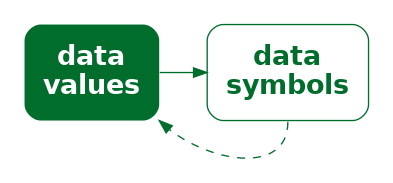
\includegraphics[scale=0.5]{Diagrams/data-sym-decode.png}

}

\caption{\label{fig-decode}The effectiveness of a data visualisation
will depend on how well our visual system can \textbf{decode} from the
data symbols to the properties of the data.}

\end{figure}%

\section{The eye}\label{sec-eye}

In order for us to perceive a data visualisation, light must emit from a
computer screen or reflect off a page and enter the eye. Light passes
through the pupil, is focused by the lens, and is projected onto the
retina at the back of the eye. The retina contains around 100 million
light-sensitive nerve cells and signals from those are combined into
about 1 million nerve fibres in the optic nerve, which passes signals on
to the brain (see Figure~\ref{fig-eye}). A very large amount of visual
information is gathered by the eye and passed on to the brain.

\begin{figure}

\centering{

\pandocbounded{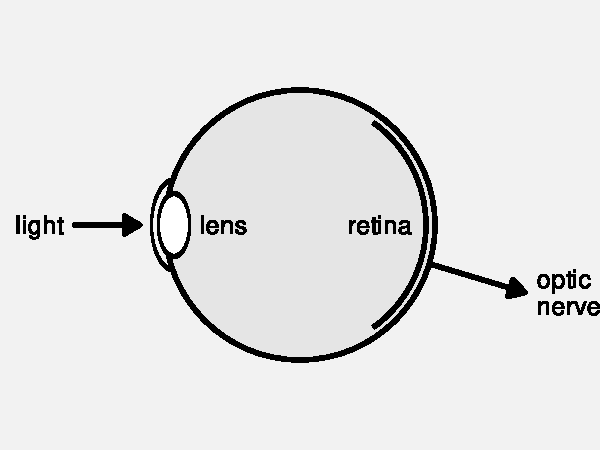
\includegraphics[keepaspectratio]{index_files/mediabag/Figures/eye-basic.pdf}}

}

\caption{\label{fig-eye}A very simple diagram of the human eye. Light
enters via the pupil and is focused by the lens onto retina.
Light-sensitive neurons in the retina pass signals via the optic nerve
to the brain.}

\end{figure}%

\begin{quote}
Data visualisation is effective because the visual system gathers an
enormous amount of information.
\end{quote}

\section{Visual focus}\label{visual-focus}

Figure~\ref{fig-eye-2} shows a slightly more detailed view of the
structure of the eye (compared to Figure~\ref{fig-eye}). The retina
contains two types of light-sensitive cells: \textbf{cones} and
\textbf{rods}. The cones are sensitive to colour and are concentrated
very densely at the centre of the retina, in an area called the
\textbf{fovea}. Rods only detect the amount of light (monochrome vision)
and are spread more sparsely towards the periphery of the retina.

This arrangement means that, despite the experience of a complete,
detailed field of view, we only get detailed and colourful information
from a small foveal region (less than 5 degrees of visual angle). The
information from our peripheral vision is less colourful and
lower-resolution.\footnote{This is not to say that peripheral vision is
  useless. Peripheral vision contributes significantly to our field of
  view (Stewart, Valsecchi, and Schütz 2020; Rosenholtz 2016), and is as
  capable as foveal vision at detecting motion (Mckee and Nakayama
  1984). However, our ability to perceive fine details is limited to a
  relatively small area of focus.}

\begin{figure}

\centering{

\pandocbounded{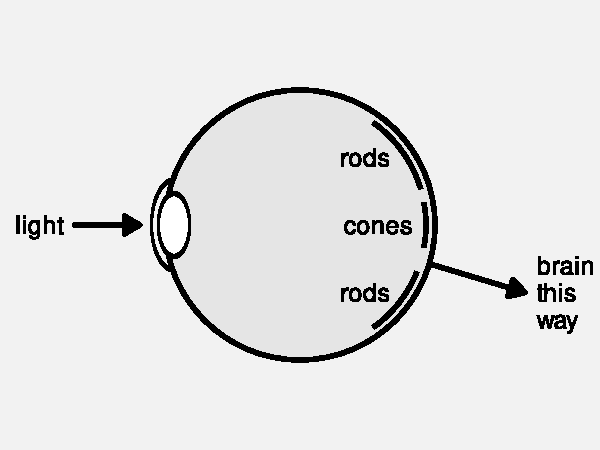
\includegraphics[keepaspectratio]{index_files/mediabag/Figures/eye-basic-2.pdf}}

}

\caption{\label{fig-eye-2}A slightly less simple diagram of the human
eye. There are two kinds of light-sensitive cells in the retina. Cones
are colour-sensitive and focused very densely at the centre of the
retina. Rods are only light-sensitive and are spread less densely
towards the periphery of the retina.}

\end{figure}%

Furthermore, when we view an image, we do not simply stare at the centre
and see everything. Instead, we perform a series of \textbf{fixations},
which are brief periods of focus on one area of the image, with
\textbf{saccades} in between, which are rapid changes in the location of
our focus. Figure~\ref{fig-extinction} demonstrates that where we look
within an image makes a difference.\footnote{The extinction illusion is
  related to the Hermann grid illusion (Ninio and Stevens 2000).

  This illusion is not explained simply by differences in foveal versus
  peripheral perception---there is currently no complete explanation for
  the effect---but it serves to show that we are getting different
  information from different regions of the field of view.}

\begin{figure}

\centering{

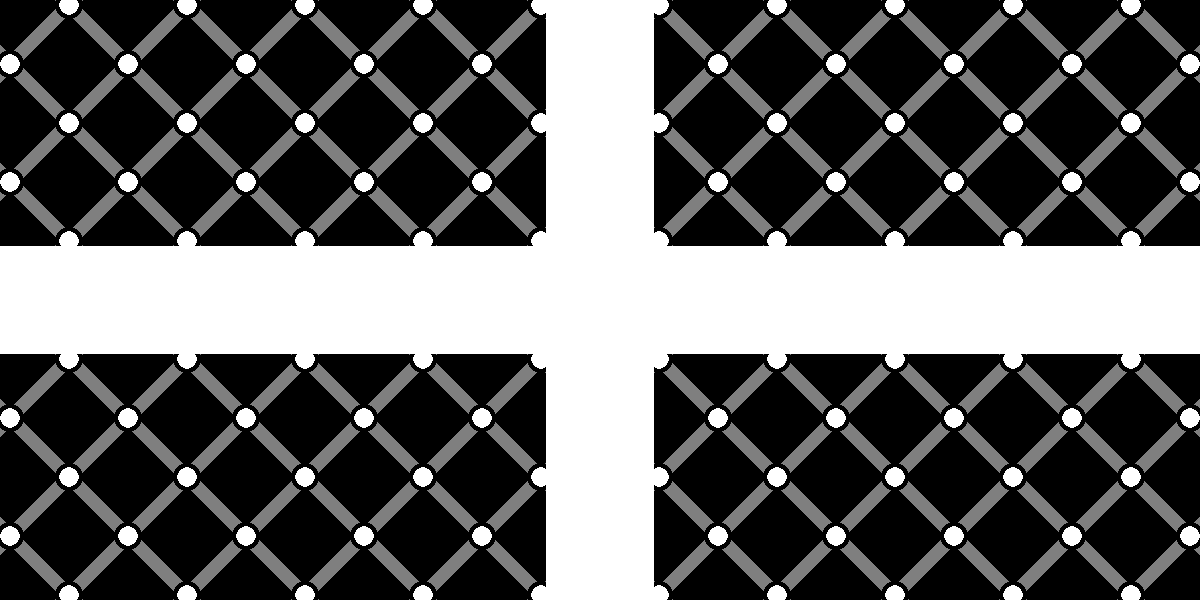
\includegraphics[width=1\linewidth,height=\textheight,keepaspectratio]{index_files/mediabag/visual-model_files/figure-pdf/fig-extinction-1.pdf}

}

\caption{\label{fig-extinction}The extinction illusion. Look at one
corner of the image and then switch focus to a different corner of the
image. At a certain viewing distance, the white dots should disappear
when we are not focused on them. We may also see black dots within the
white dots in our peripheral vision.}

\end{figure}%

Figure~\ref{fig-fixations} shows eye-tracking data from one person
viewing an image for 10 seconds.\footnote{The plot was originally from
  The Economist, but this image was taken from the resources provided on
  the \href{http://massvis.mit.edu/}{MASSVIS project web site}. The eye
  tracking data were taken from the same web site. Cite MASSVIS article.
  Only a thumbnail version of the original image is shown in
  Figure~\ref{fig-fixations} in order to comply with terms of use of the
  MASSVIS data set.} The original image is shown on the left and
eye-tracking data is shown on the right, with hollow black circles
showing the position of the coloured circles in the original image. In
the eye-tracking image, the fixations are shown as purple circles and
the saccades are shown as lines between the circles. For example, we can
see that the viewer has fixated multiple times upon the large, colourful
circles in the original image and also text at the top and bottom of the
image.

\begin{figure}

\begin{minipage}{0.50\linewidth}

\pandocbounded{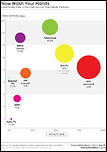
\includegraphics[keepaspectratio]{MASSVIS/visMost505-thumb.png}}

\subcaption{\label{fig-fixations-1}A thumbnail of the original image.}

\end{minipage}%
%
\begin{minipage}{0.50\linewidth}

\pandocbounded{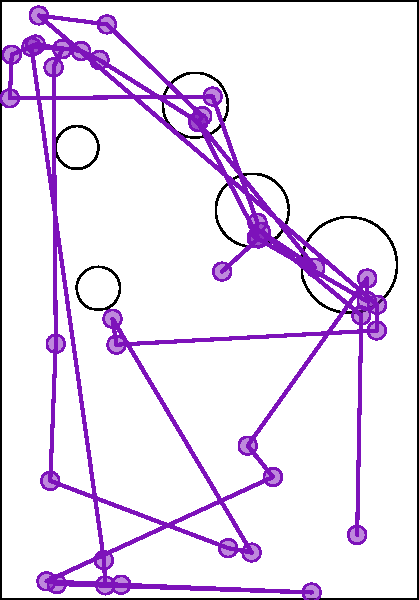
\includegraphics[keepaspectratio]{index_files/mediabag/MASSVIS/visMost505-track.pdf}}

\subcaption{\label{fig-fixations-2}Fixations and saccades from
eye-tracking data.}

\end{minipage}%

\caption{\label{fig-fixations}Eye tracking data (on the right) from the
MASSVIS project that shows fixations (circles) and saccades (lines
between circles) for one person viewing an image for 10 seconds. A
thumbnail of the original image is shown on the left.}

\end{figure}%

\begin{quote}
A data visualisation may be require more effort to decode if it contains
many different areas of detail that require the viewer to constantly
switch focus.
\end{quote}

\section{Visual memory}\label{visual-memory}

When we switch focus to different areas of an image, we are likely to
need to remember information from a previous area of focus. How well can
we hold visual information in memory? The most important feature of
visual memory is that it is very limited. We can only hold in memory a
small number of items at once.\footnote{And footnote that acknowledges
  some controversy (different models and number of items limit vs
  continuous resource limit), with ref to e.g., ``Psychophysical scaling
  reveals a unified theory of visual memory strength'' Schurgin et al
  (2020) and the binary map model

  Some limitations of visual memory are briefly mentioned in Ware (2021)
  (pp.~397-405 and pp.~423-425).}

\afterpage{
\begin{figure}[t]
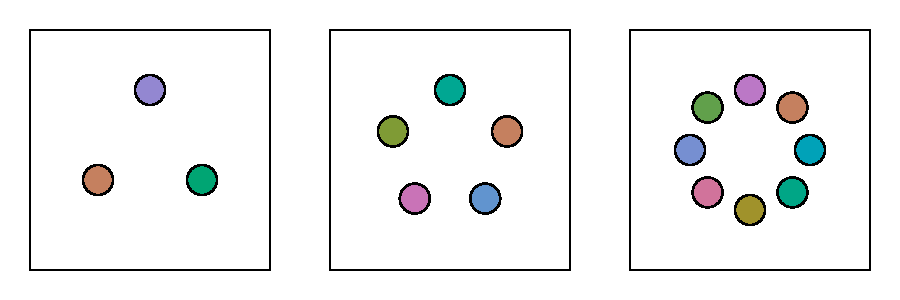
\includegraphics{Memory/static-1.pdf}

\caption{\label{fig-memory-static-1}
A memory task.  Focus on the circles in one of the three squares
then turn the page and try to tell how many of the circles have
changed colour in the corresponding square in @fig-memory-static-2.
The task should be obviously harder when there are more circles
to remember, which reflects the limits on visual memory.}
\end{figure}
}

\afterpage{
\begin{figure}[t]
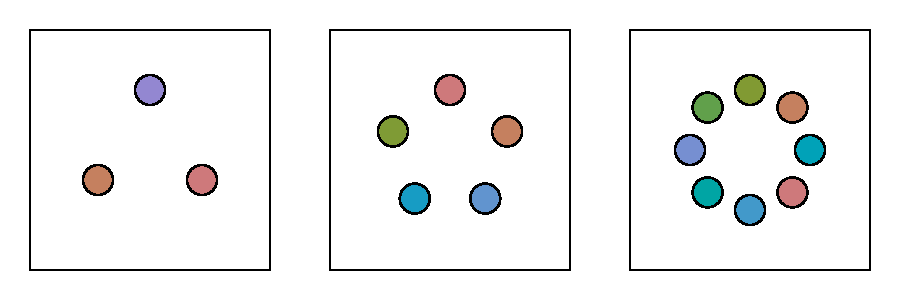
\includegraphics{Memory/static-2.pdf}

\caption{\label{fig-memory-static-2}
A memory task.  Look at the circles in one of the squares
in @fig-memory-static-1 on the previous page and then come
back here and try to tell how many circles have changed colour
in the corresponding square.
The task should be obviously harder when there are more circles
to remember, which reflects the limits on visual memory.}
\end{figure}
}

It is easier and faster to decode information from visual elements if
they lie within the scope of a single visual focus. If we have to switch
focus, it not only takes longer to decode information, but we may hit
limits on our ability to remember visual elements from previous areas of
focus.\footnote{Tufte refers to this as drawing ``within the eyespan''
  (Tufte 1990, 67)

  ``In understanding human visual perception, an important component
  consists of what people can perceive at a glance. If that glance
  provides the observer with sufficient task-relevant information, this
  affords efficient processing. If not, one must move one's eyes and
  integrate information across glances and over time, which is
  necessarily slower and limited by both working memory and the ability
  to integrate that information.'' (Rosenholtz 2023).}

\begin{quote}
A data visualisation will require more effort to decode if the viewer is
required to switch focus and retain information across multiple areas of
visual focus.
\end{quote}

\section{Visual processing}\label{sec-visual-processing}

Processing of the signals from the optic nerve occurs in several areas
of the brain. Very basic \textbf{visual features} are extracted first,
such as \textbf{position} (spatial arrangements), \textbf{angle}
(orientations), \textbf{colour}, and simple \textbf{patterns} (spatial
frequencies). This low-level information is passed on and built upon to
produce higher-level representations, such as regions and
\textbf{shapes}. Information is then also integrated from prior
knowledge to assist with the identification of \textbf{objects}---things
like trees, animals, and faces.\footnote{cite Ware (4th) p229-330, also
  fig 6.1}

\begin{figure}

\centering{


\includegraphics[scale=0.5]{Diagrams/visual-processing.png}

}

\caption{\label{fig-visual-processing}A very simple model of visual
processing.}

\end{figure}%

Lower-level processing occurs subconsciously and more rapidly than
higher-level processing, which can require conscious effort.
Furthermore, lower-level processing occurs in parallel and can involve
many instances of visual features at once, whereas higher-level
processing will only focus on a small number of items or a single item
at once. On the other hand, lower-level visual features are rapidly
discarded as our attention shifts, while higher-level visual objects are
more persistent and may become part of long-term memories (see
Figure~\ref{fig-visual-model}).

\begin{figure}

\centering{

\pandocbounded{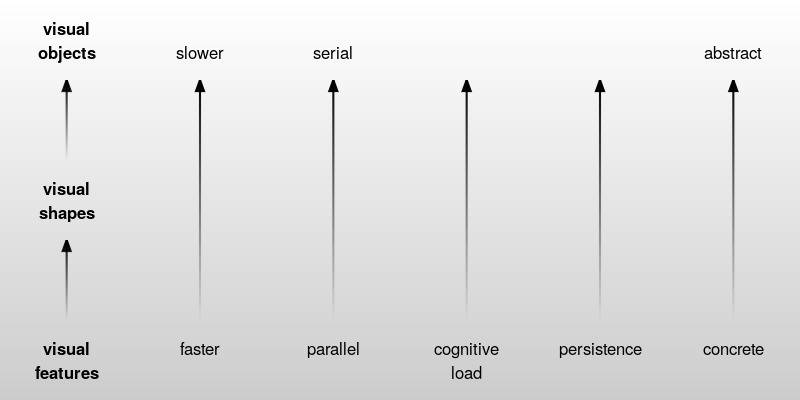
\includegraphics[keepaspectratio]{Model/model.png}}

}

\caption{\label{fig-visual-model}Some of the properties of visual
processing.}

\end{figure}%

Figure~\ref{fig-visual-model-demo} shows an image that is made up of
many small items: tiny triangles with different \textbf{lengths},
orientations (\textbf{angles}), and \textbf{colours}. The orientations
of the triangles represents wind direction and the length of the
triangles represents wind strength; blue triangles are over the sea and
green triangles are over land.\footnote{Figure~\ref{fig-visual-model-demo}
  is based on wind data from the National Oceanic and Atmospheric
  Administration's Operational Model Archive and Distribution System
  (\href{https://nomads.ncep.noaa.gov/}{NOMADS}). The data were accessed
  and processed using the \{rNOMADS\} package (Bowman and Lees 2015),
  with raw data interpolated to a finer grid.} The visual system can
very quickly perceive many small \textbf{visual features} at once. There
is no need to concentrate separately on every individual triangle in the
image.. At a higher level of processing, darker and lighter
\textbf{regions} are identified as well as regions of different colours.
For example, a band of lighter wind forms a line from the top-left
corner at a roughly 45-degree angle. At a higher level of processing
again, at least for the denizens of Oceania, the green regions are
recognised as a very familiar \textbf{object}: the outline of New
Zealand.

The small lines convey a lot of simple pieces of information---what is
the wind strength and direction at each location---though we have to
focus on a particular spot in order to extract that information. The
darker and lighter regions convey several more complex ideas like
regions of stronger and lighter winds. The green regions combine to
convey the single complex and abstract concept of New Zealand.

\begin{figure}

\centering{

\pandocbounded{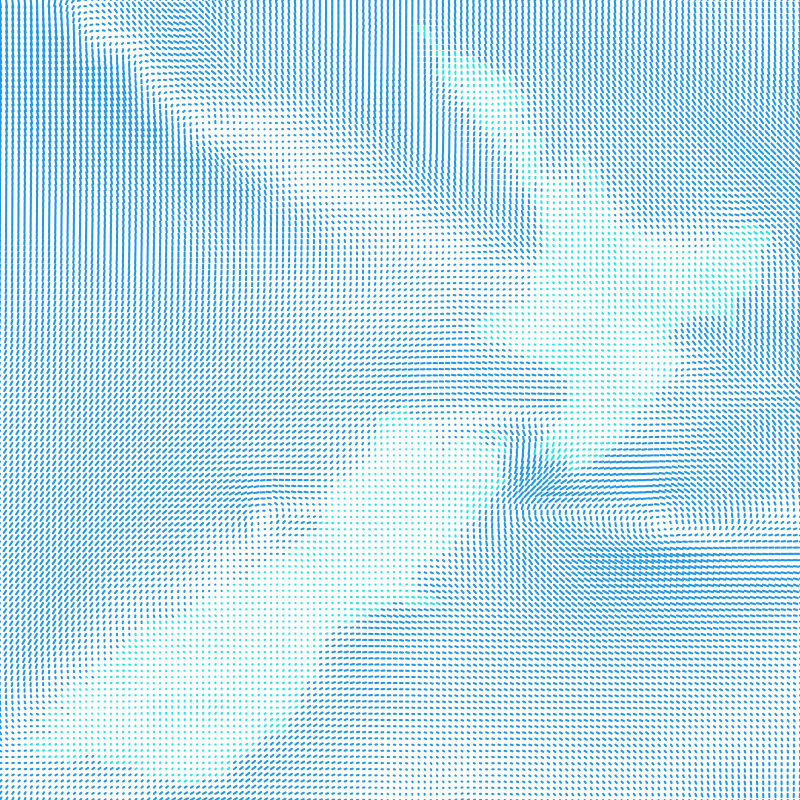
\includegraphics[keepaspectratio]{Data/Weather/NOMADS.png}}

}

\caption{\label{fig-visual-model-demo}A visualisation of wind strength
and wind direction that is made up of lots of small lines of different
lengths and different angles and different colours.}

\end{figure}%

\section{Visual differences}\label{sec-differences}

The ability to gather a large amount of basic features from an image
very quickly is supplemented by rapid visual processing that combines
and summarises the information. These subconscious processes extract
some properties from an image without any mental effort.

For example, in Figure~\ref{fig-pop-colour-1} we can detect the one teal
dot amongst the 24 orange dots without effort.
Figure~\ref{fig-pop-colour-2} shows that this task remains effortless
even if the number of distractors is much larger.\footnote{Mention
  ``pre-attentive'' plus citations.}

\begin{figure}

\begin{minipage}{0.50\linewidth}

\centering{

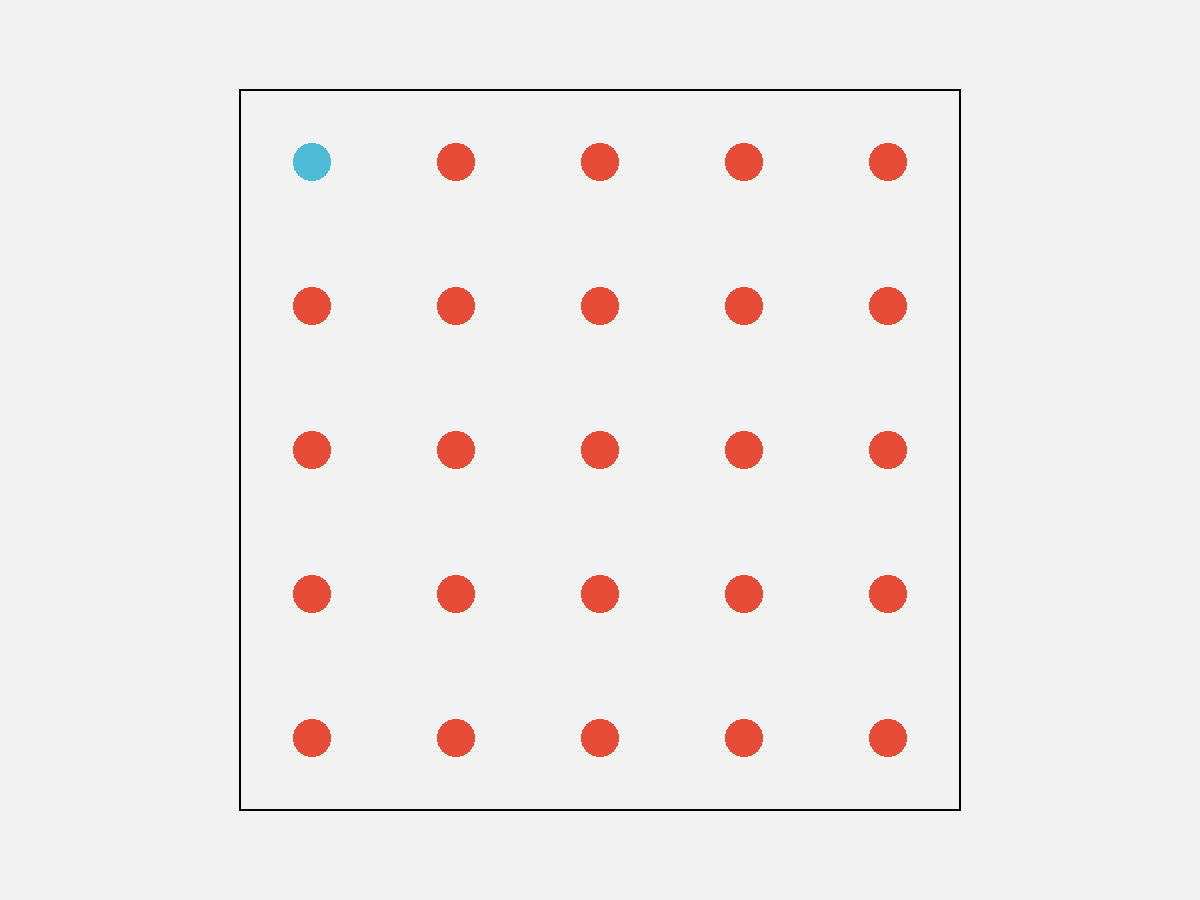
\includegraphics[width=1\linewidth,height=\textheight,keepaspectratio]{index_files/mediabag/visual-model_files/figure-pdf/fig-pop-colour-1.pdf}

}

\subcaption{\label{fig-pop-colour-1}One teal dot amongst 24 orange
dots.}

\end{minipage}%
%
\begin{minipage}{0.50\linewidth}

\centering{

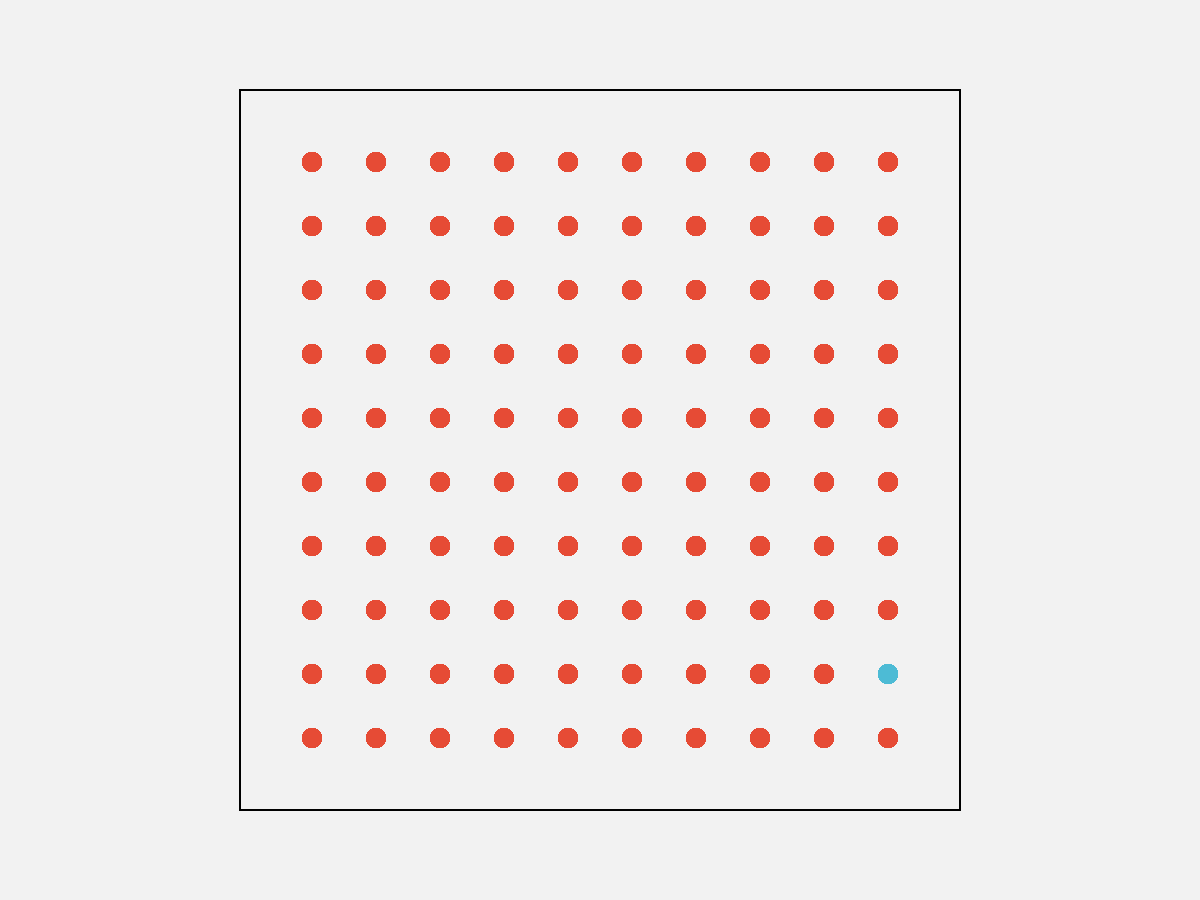
\includegraphics[width=1\linewidth,height=\textheight,keepaspectratio]{index_files/mediabag/visual-model_files/figure-pdf/fig-pop-colour-2.pdf}

}

\subcaption{\label{fig-pop-colour-2}One teal dot amongst 99 orange
dots.}

\end{minipage}%

\caption{\label{fig-pop-colour}Amongst a collection of dots, we
effortlessly perceive one dot that has a different colour.}

\end{figure}%

This ability to identify an item that is different from all other items
within an image also applies to other basic features like size, as shown
in Figure~\ref{fig-diff-size}.

\begin{figure}

\begin{minipage}{0.50\linewidth}

\centering{

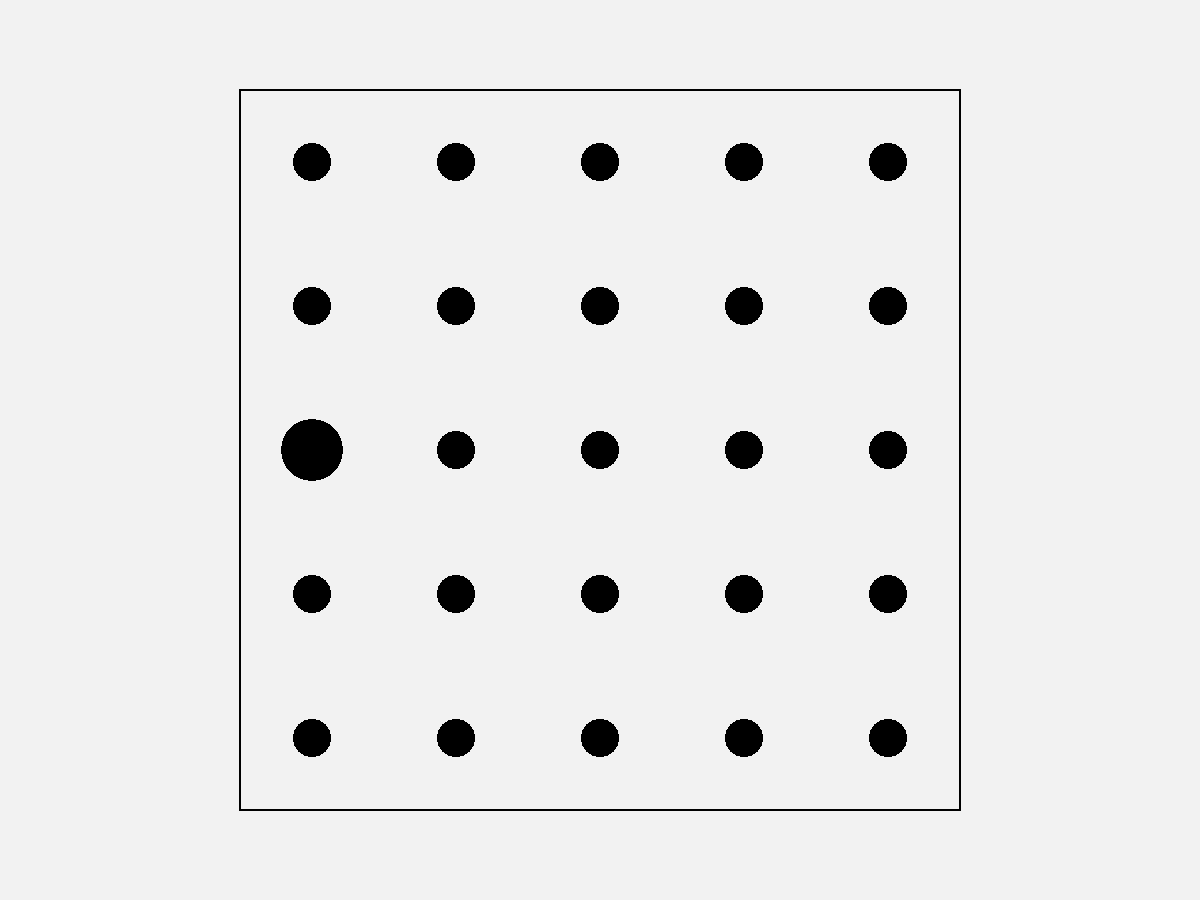
\includegraphics[width=1\linewidth,height=\textheight,keepaspectratio]{index_files/mediabag/visual-model_files/figure-pdf/fig-diff-size-1.pdf}

}

\subcaption{\label{fig-diff-size-1}One larger dot amongst 24 smaller
dots.}

\end{minipage}%
%
\begin{minipage}{0.50\linewidth}

\centering{

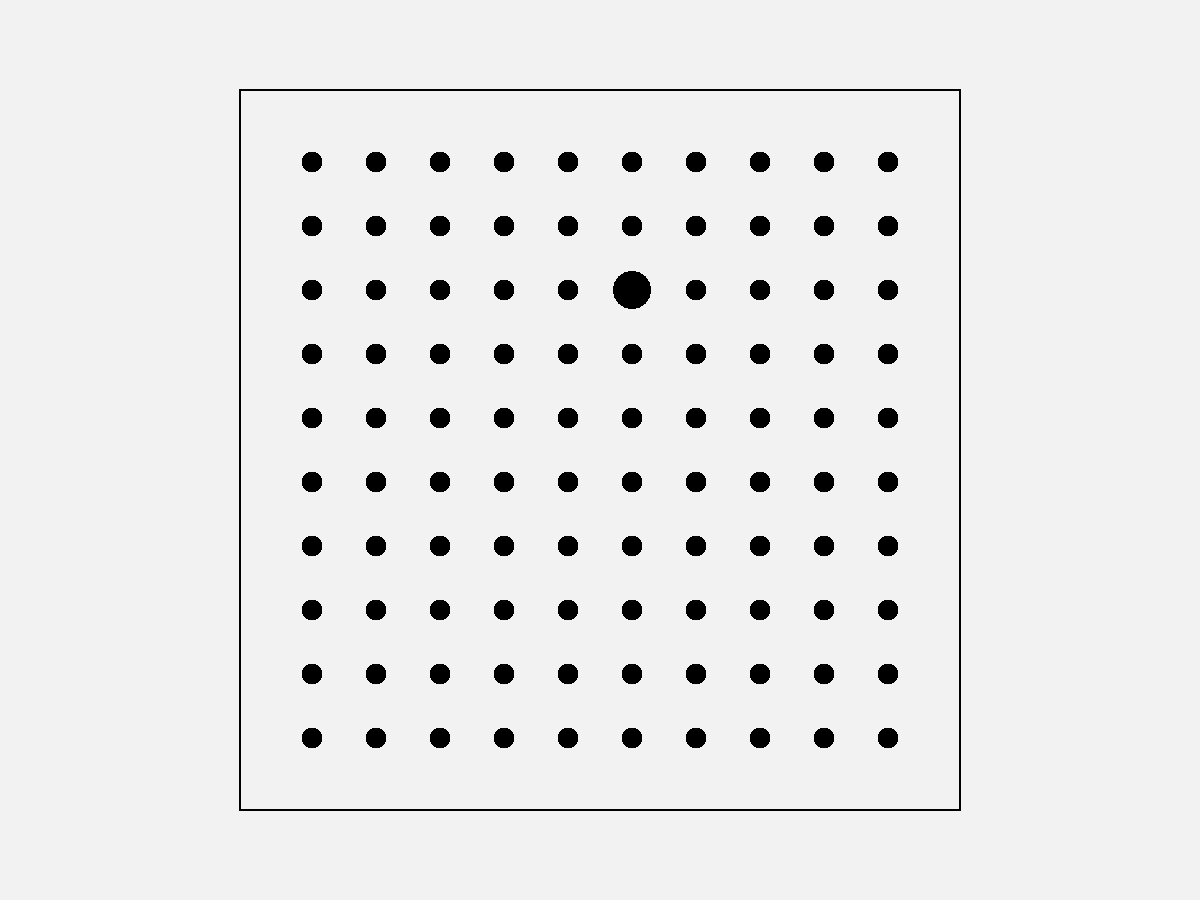
\includegraphics[width=1\linewidth,height=\textheight,keepaspectratio]{index_files/mediabag/visual-model_files/figure-pdf/fig-diff-size-2.pdf}

}

\subcaption{\label{fig-diff-size-2}One larger dot amongst 99 smaller
dots.}

\end{minipage}%

\caption{\label{fig-diff-size}Amongst a collection of dots, we
effortlessly perceive one dot that differs only by size.}

\end{figure}%

If an item differs on more than one visual feature, the effect is even
stronger (Figure~\ref{fig-diff-salience}). The visual system is very
sensitive to items that are \textbf{different} in terms of basic
\textbf{visual features}.

\begin{figure}

\begin{minipage}{0.50\linewidth}

\centering{

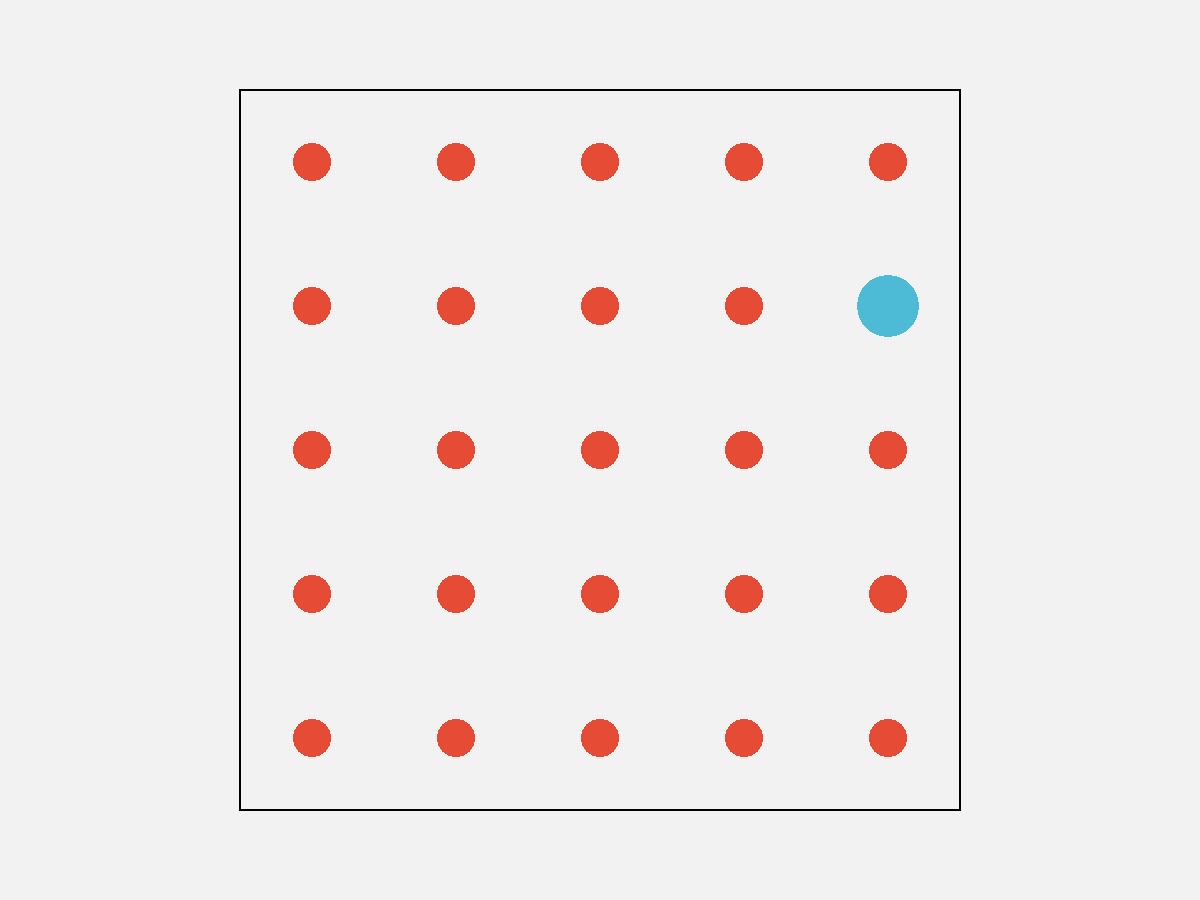
\includegraphics[width=1\linewidth,height=\textheight,keepaspectratio]{index_files/mediabag/visual-model_files/figure-pdf/fig-diff-salience-1.pdf}

}

\subcaption{\label{fig-diff-salience-1}One larger teal dot amongst 24
smaller orange dots.}

\end{minipage}%
%
\begin{minipage}{0.50\linewidth}

\centering{

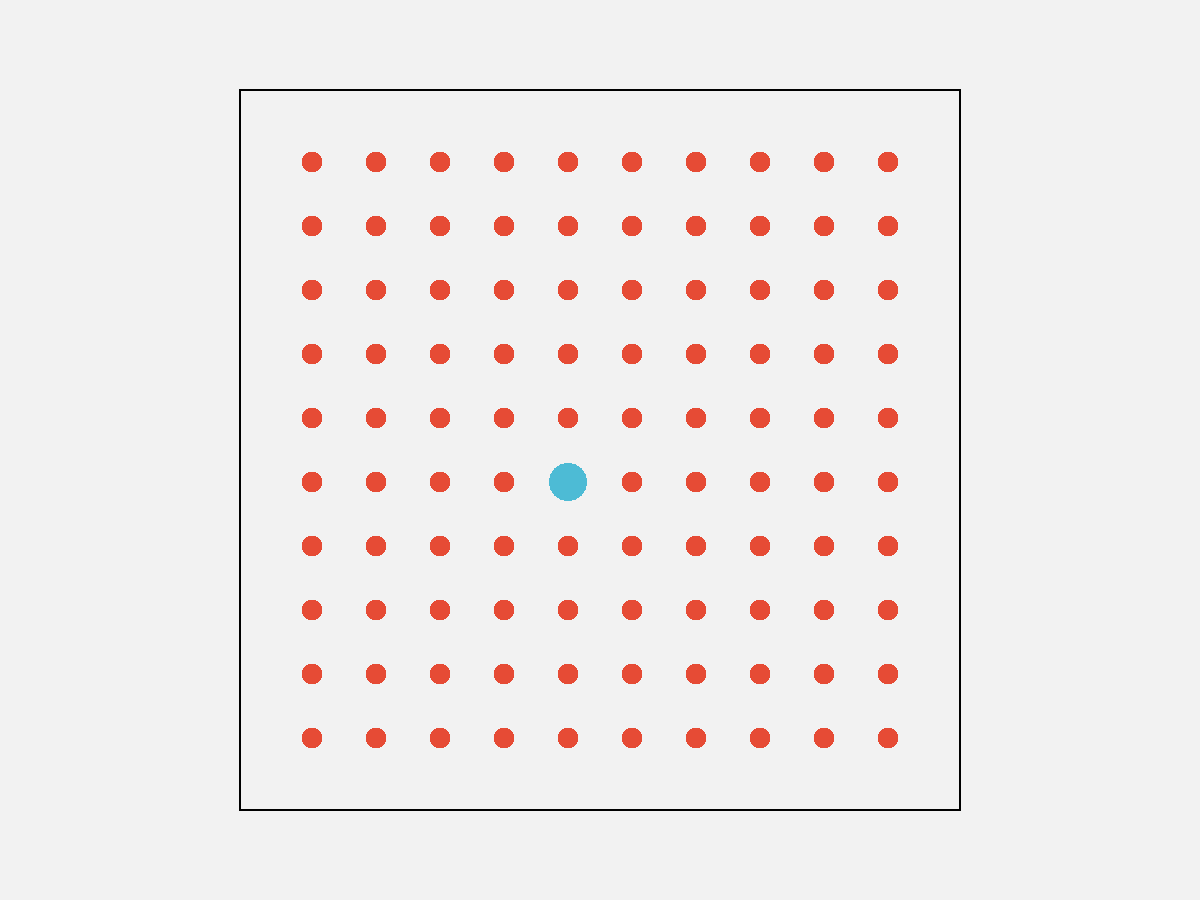
\includegraphics[width=1\linewidth,height=\textheight,keepaspectratio]{index_files/mediabag/visual-model_files/figure-pdf/fig-diff-salience-2.pdf}

}

\subcaption{\label{fig-diff-salience-2}One larger teal dot amongst 99
smaller orange dots.}

\end{minipage}%

\caption{\label{fig-diff-salience}Amongst a collection of dots, we
effortlessly perceive one dot that differs by both colour and size.}

\end{figure}%

On the other hand, if the distractor items are both similar on one
visual feature, but different on another, and if the arrangement of the
items is less structured, then finding a particular item of interest
becomes much harder. For example, if we look for the single larger teal
dot in Figure~\ref{fig-diff-serial}, it is much harder to find than it
is in Figure~\ref{fig-diff-salience}. The visual system's sensitivity to
\textbf{different} items is much greater when all other items are the
\textbf{same}.\footnote{We hang our hat on this several times later on,
  so it would be good to ground it in the literature!!!}

\begin{figure}

\begin{minipage}{0.50\linewidth}

\centering{

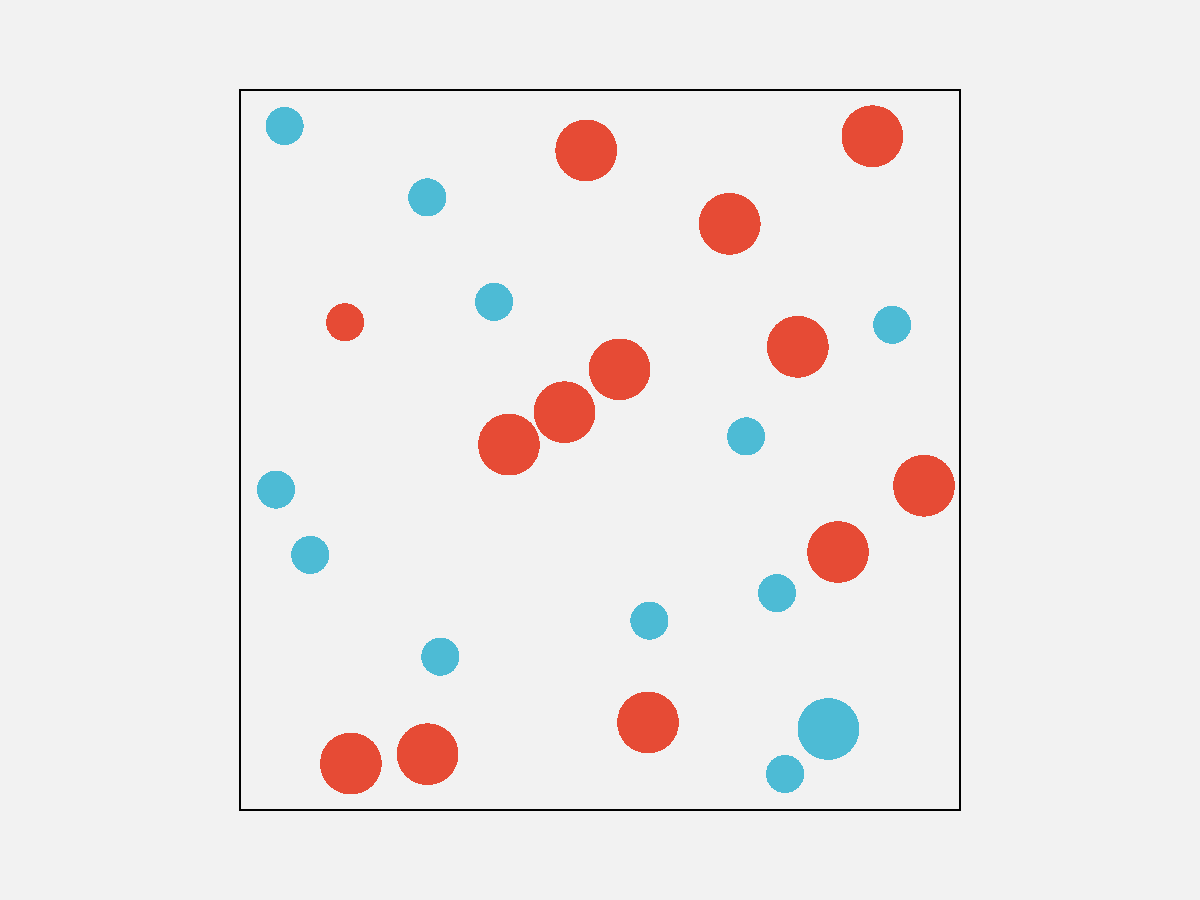
\includegraphics[width=1\linewidth,height=\textheight,keepaspectratio]{index_files/mediabag/visual-model_files/figure-pdf/fig-diff-serial-1.pdf}

}

\subcaption{\label{fig-diff-serial-1}One larger teal dot amongst 24 dots
that differ by colour and/or size.}

\end{minipage}%
%
\begin{minipage}{0.50\linewidth}

\centering{

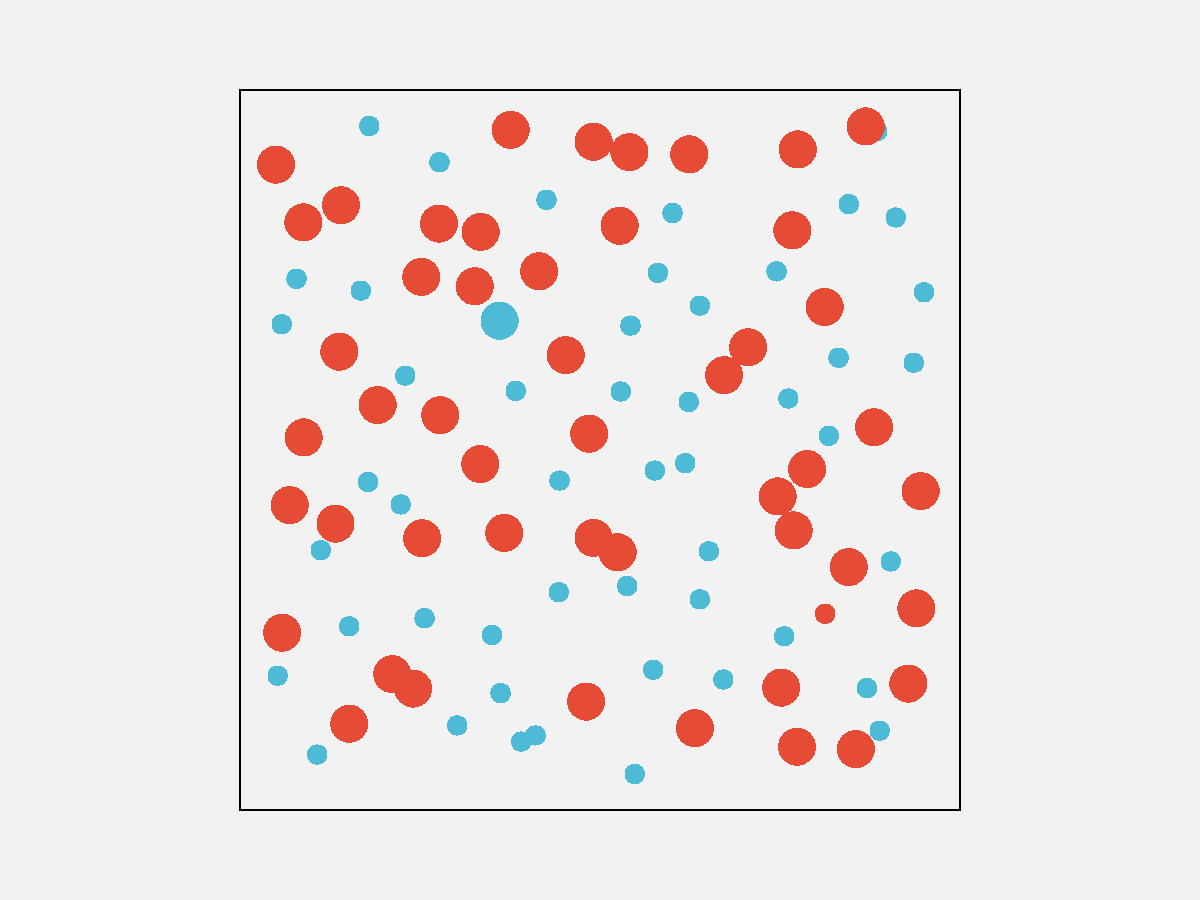
\includegraphics[width=1\linewidth,height=\textheight,keepaspectratio]{index_files/mediabag/visual-model_files/figure-pdf/fig-diff-serial-2.pdf}

}

\subcaption{\label{fig-diff-serial-2}One larger teal dot amongst 99 dots
that differ by colour and/or size.}

\end{minipage}%

\caption{\label{fig-diff-serial}We have to work much harder when there
is more going on.}

\end{figure}%

\section{Visual attention}\label{sec-attention}

Where we focus within an image is not random.\footnote{Citation to
  bottom-up vs top-down.} The figures from Section~\ref{sec-differences}
show that our attention is automatically drawn to the \textbf{larger},
\textbf{brighter}, and more \textbf{colourful} items within an image.
This happens due to very early visual processing and without conscious
thought.

Where we focus within an image, and what information we extract, is also
affected by conscious goals---what are we looking for?\footnote{Citation
  to mentions of attention filtering visual input differently} For
example, when you were looking for the larger teal dot in
Figure~\ref{fig-diff-serial}, did you notice that there was also a
single small orange dot? Now that your attention has been drawn to that
task, it will be easier to find the smaller orange dot.

\section{Visual similarities}\label{sec-visual-model-groups}

In Figure~\ref{fig-diff-serial}, we can see several groups of items:
orange dots, teal dots, large dots, and small dots. These separate
groups of items are identified based on their \textbf{similarity}---each
group of items have the same size and the same colour.

As with the detection of differences that we saw in
Section~\ref{sec-differences}, the grouping of similar items within an
image happens automatically and without conscious effort. Furthermore,
there are other visual properties that mean we automatically perceive
items as groups: items that are close together (items that have similar
\textbf{positions}) are seen as a group; items that are connected by
lines are seen as a group; and items that are enclosed by a border or
background are seen as a group.\footnote{mention Gestalt ``school'' or
  whatever, plus citations. enclosure == common region ``Gestalt
  principles'' Todorovic (2008) Summaries of the main Gestalt
  principles. Like a peer-reviewed Wikipedia ? Possible link to
  alignment \ldots{} ? ``good Gestalt principle: elements tend to be
  grouped together if they are parts of a pattern which is a good
  Gestalt, meaning as simple, orderly, balanced, unified, coherent,
  regular, etc as possible''}

For example, in Figure~\ref{fig-gestalt-group} there are several
matrices of dots. In each matrix, we can see either rows of dots or
columns of dots by manipulating visual features that affect our
perception of groups: dots that are closer together for a group; dots
that are the same colour form a group; dots that are connected by lines
form a group.

\begin{figure}

\centering{


\includegraphics[width=1\linewidth,height=\textheight,keepaspectratio]{index_files/mediabag/visual-model_files/figure-pdf/fig-gestalt-group-1.pdf}

}

\caption{\label{fig-gestalt-group}In each matrix of dots, we clearly see
either rows or columns. In the pair of matrices on the left, making the
dots slightly closer together horizontally produces rows, and making the
dots slightly closer vertically produces columns. In the middle pair of
matrices, using the same colour on each row produces rows, and using the
same colour on each column produces columns. In the pair of matrices on
the right, drawing vertical lines produces columns and drawing
horizontal lines produces rows.}

\end{figure}%

These grouping effects are very powerful and can even be used to
override each other in some combinations. Figure~\ref{fig-gestalt-group}
shows that an enclosing border can be stronger than a connecting line,
connecting lines can be stronger than closeness, and closeness can be
stronger than similar colours.

\begin{figure}

\centering{

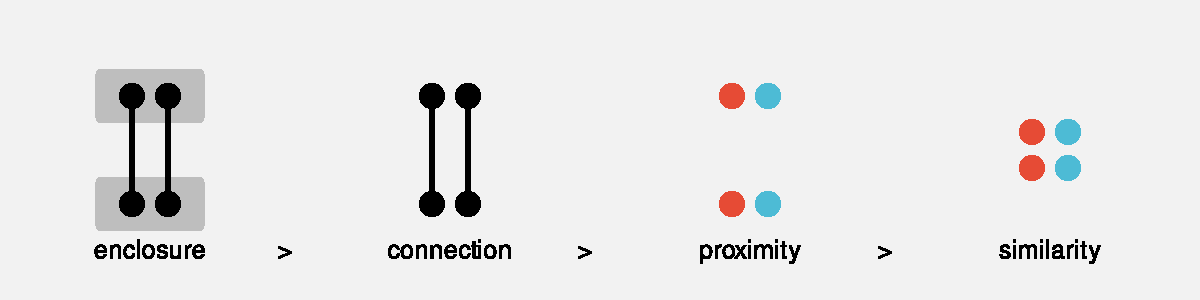
\includegraphics[width=1\linewidth,height=\textheight,keepaspectratio]{index_files/mediabag/visual-model_files/figure-pdf/fig-gestalt-order-1.pdf}

}

\caption{\label{fig-gestalt-order}For each set of four dots, we
automatically perceive two pairs of dots. On the left, the enclosing
grey rectangles produce an upper pair and a lower pair. Second from
left, the lines produce a left pair and a right pair. Second from right,
closeness produces an upper pair and a lower pair. On the right, colour
produces a left pair and a right pair.}

\end{figure}%

Another type of automatic grouping is demonstrated in
Figure~\ref{fig-continuity}. On the left is a collection of dots. We
naturally perceive a horizontal line and a circle from these dots, as
shown in the centre of Figure~\ref{fig-continuity}. We automatically
complete lines, particularly smooth curves, even when the curve is
broken, as in the central set of dots. We do not tend to complete lines
with sharp corners, as indicated on the right of
Figure~\ref{fig-continuity}.\footnote{Gestalt continuity cite.}

\begin{figure}

\centering{


\includegraphics[width=1\linewidth,height=\textheight,keepaspectratio]{index_files/mediabag/visual-model_files/figure-pdf/fig-continuity-1.pdf}

}

\caption{\label{fig-continuity}We automatically complete curves.}

\end{figure}%

When we visualise qualitative data, we will be able to rely on the
automatic identification of different groups of data symbols based on
visual similarities.

\begin{quote}
A data visualisation of qualitative data may be effective if it relies
on the automatic identification of visual groups (proximity, similarity,
etc).
\end{quote}

\section{Visual simplicity}\label{sec-simplicity}

Figure~\ref{fig-simplicity} shows an arrangement of dots, similar to
Figure~\ref{fig-continuity}. The collection of dots on the left has an
ambiguous interpretation. Is this a single shape, or two overlapping
shapes (as indicated in the centre of Figure~\ref{fig-simplicity}), or
some complex combination of multiple shapes (as indicated on the right
of Figure~\ref{fig-simplicity})?

Our visual system has a preference for the simple interpretation. Given
an ambiguous arrangement of visual elements, we will tend to perceive
whatever is most orderly, regular, and coherent.\footnote{Good gestalt
  and prägnanz cite}

\begin{figure}

\centering{


\includegraphics[width=1\linewidth,height=\textheight,keepaspectratio]{index_files/mediabag/visual-model_files/figure-pdf/fig-simplicity-1.pdf}

}

\caption{\label{fig-simplicity}We automatically perceive simple shapes
over more complex interpretations.}

\end{figure}%

Figure~\ref{fig-symmetry} shows that we also perceive groups when items
have a symmetric arrangement.

\begin{figure}

\centering{

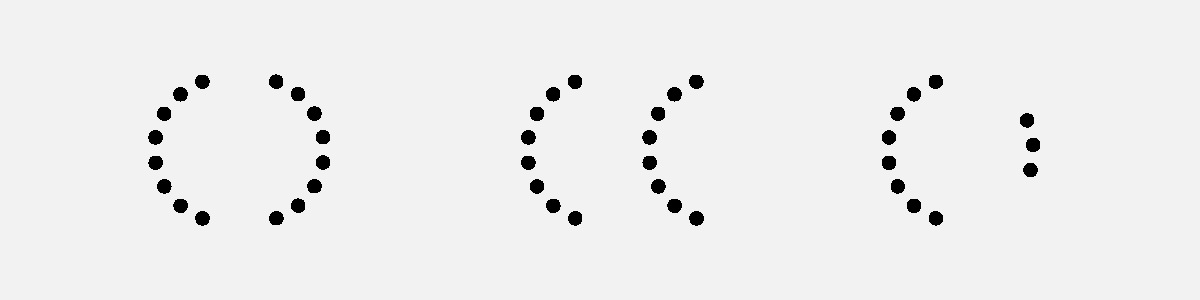
\includegraphics[width=1\linewidth,height=\textheight,keepaspectratio]{index_files/mediabag/visual-model_files/figure-pdf/fig-symmetry-1.pdf}

}

\caption{\label{fig-symmetry}We automatically perceive groups from
symmetric arrangements.}

\end{figure}%

These results suggest that a data visualisations will be more effective
if it is simple and orderly. We should lead the viewer where they
already want to go rather than trying to force the viewer to perceive a
more complex interpretation.

\begin{quote}
A data visualisation may be effective if it is orderly and lends itself
to a simple interpretation.
\end{quote}

\section{Visual tasks}\label{sec-tasks}

Identifying whether visual elements are the same or different
(Section~\ref{sec-differences}) is an example of a very simple visual
task. Figure~\ref{fig-visual-task} (on the left) shows another simple
visual task: judging the ratio of different lengths. However, on the
right of Figure~\ref{fig-visual-task} is an example of a task that is
much more difficult. In this task, we have to identify which of the four
shapes in the bottom row is \emph{not} a rotated version of the shape at
the top.

\begin{figure}

\centering{

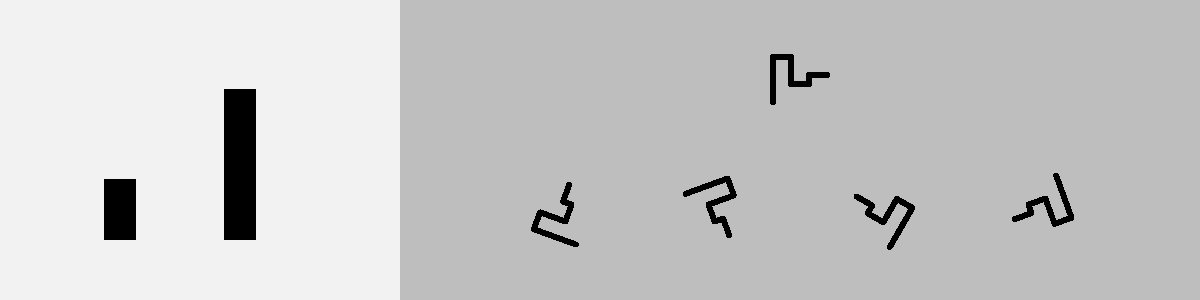
\includegraphics[width=1\linewidth,height=\textheight,keepaspectratio]{index_files/mediabag/visual-model_files/figure-pdf/fig-visual-task-1.pdf}

}

\caption{\label{fig-visual-task}On the left is a simple visual task, to
estimate the relative length of the two lines. On the right is a more
complicated visual task, to decide which of the four bottom shapes is
\emph{not} a rotated version of the top shape.}

\end{figure}%

The left-hand task in Figure~\ref{fig-visual-task} is effortless and can
be performed immediately. The right-hand task in
Figure~\ref{fig-visual-task} requires much more deliberate effort and
time to perform.

One way to create an effective data visualisation is to rely on visual
tasks that are rapid and require little effort.

\section{The dangers of the visual
system}\label{the-dangers-of-the-visual-system}

Visual illusions.

The fact that vertical lines appear longer than horizontal lines is a
good simple one to demonstrate and relate to data vis (both L and T
versions).

\section{Summary}\label{summary-1}

The human visual system captures a very large amount of information from
the visual field.

Detailed information is only available at the centre of the visual field
so multiple fixations are required to capture detailed information from
multiple locations within an image.

Large numbers of simple features are rapidly extracted, while more
complex visual items take longer and require more congnitive effort, but
persist for longer.

Large, bright, colourful items automatically stand out.

Items are automatically grouped in terms of similarity (of basic visual
features), proximity, connection, and enclosure.

The main point is that the visual system is \emph{very} good at
perceiving certain visual features.

An effective data visualisation will make use of the things that the
visual system is good at.

\begin{center}\rule{0.5\linewidth}{0.5pt}\end{center}

\theendnotes

\bookmarksetup{startatroot}

\chapter{Visual Features}\label{sec-mapping-visual-features}

We have established that the mappings from data values to data symbols
are fundamental to a data visualisation. We have also established some
basic properties of the visual system and we have identified three
levels of visual processing: visual features, visual shapes, and visual
objects.

There are many possible ways to map from data values to data symbols.
For example, in Section~\ref{sec-mappings}, we saw that the same data
values could be mapped in different ways to produce different data
visualisations (Figure~\ref{fig-crime} and
Figure~\ref{fig-crime-heatmap}).

On one hand, there are many possible encodings to choose from and, on
the other hand, there are many possible data symbols to map to.

In this section, we begin to explore different sorts of mappings,
starting with the simplest case: each data value is encoded as a basic
\textbf{visual feature} of a data symbol; and \textbf{one} data value
maps to \textbf{one} data symbol (Figure~\ref{fig-visual-feature}).

\begin{figure}

\centering{

\begin{figure}[H]

\begin{minipage}{0.50\linewidth}

\includegraphics[scale=0.5]{Diagrams/data-vis.png}\end{minipage}%
%
\begin{minipage}{0.50\linewidth}
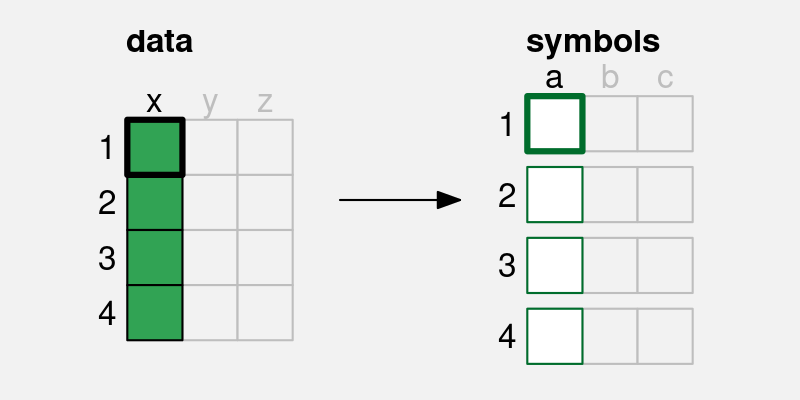
\includegraphics[scale=0.7]{Mappings/mapping-1-1-1-1.png}\end{minipage}%

\end{figure}%

}

\caption{\label{fig-visual-feature}A simple data visualisation encodes
each data value as a \textbf{visual feature} of a data symbol. Each data
value (\texttt{a}) is mapped to a visual feature (\texttt{x}) of a
single data symbol.}

\end{figure}%

\section{Bar plots}\label{bar-plots}

In order to demonstrate mapping data values to visual features, we will
work with a data visualisation of the total number of crimes for
different ethnic groups. The data values are shown in
Table~\ref{tbl-crime-group-total}.

\begin{longtable}[t]{lr}

\caption{\label{tbl-crime-group-total}A table of the total number of
offenders aged 14 to 16 from 2011 to 2021 for different ethnic groups.}

\tabularnewline

\toprule
group & total\\
\midrule
European/Other & 31274\\
Māori & 41787\\
Pasifika & 6993\\
Unknown & 5632\\
\bottomrule

\end{longtable}

A bar plot of these data is shown in Figure~\ref{fig-bar}. This is a
very effective way to visualise the total values, particularly if we are
interested in comparing the raw totals. With this data visualisation, it
is very easy to answer questions like the following:

\begin{itemize}
\tightlist
\item
  Which ethnic group has the largest total number of offenders?
\item
  Which ethnic group has the smallest total number of offenders?
\item
  Is the total number of offenders higher for Māori or Pasifika?
\item
  Is the total number of offenders for European/Other more or less than
  half the total for Māori?
\end{itemize}

\begin{figure}

\centering{

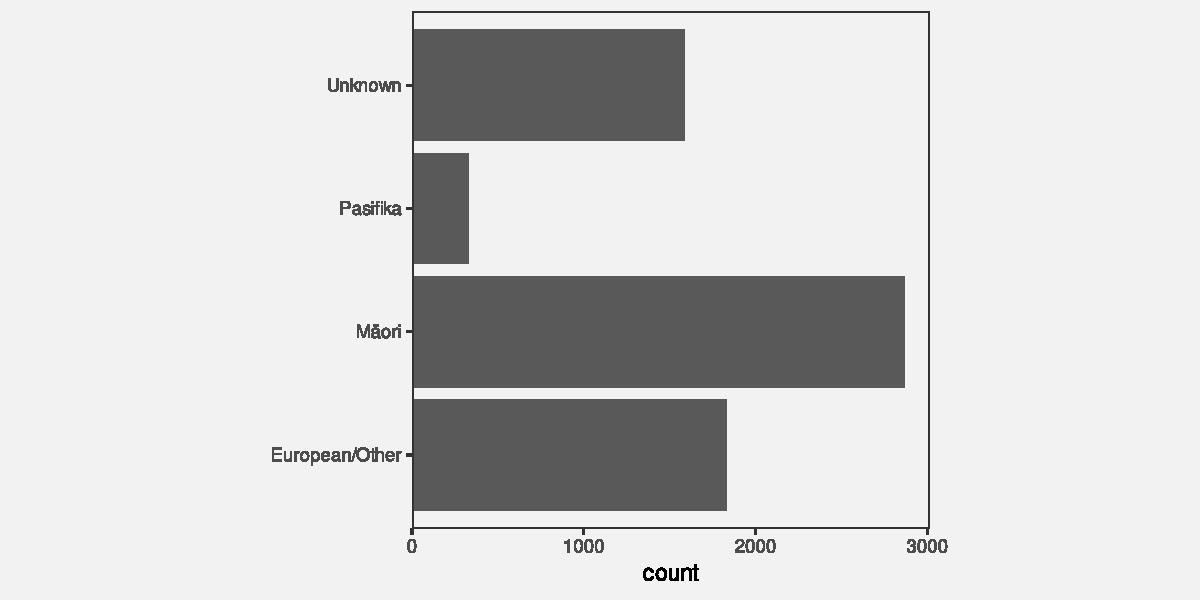
\includegraphics[width=1\linewidth,height=\textheight,keepaspectratio]{index_files/mediabag/mapping-visual-features_files/figure-pdf/fig-bar-1.pdf}

}

\caption{\label{fig-bar}A bar plot of the total number of offenders for
different ethnic groups. The data symbols in this plot are the
horizontal bars.}

\end{figure}%

Why is the data visualisation in Figure~\ref{fig-bar} so effective? To
help answer that question, we need to look at the encoding that is being
used to map the data values to data symbols.

\section{Visual features}\label{visual-features}

The data symbols in Figure~\ref{fig-bar} are a set of rectangles or
bars. However, the important visual feature of the rectangles is their
\textbf{length}; the thickness of the bars does not relate to the data
values at all (see Figure~\ref{fig-length}). The total number of crimes
for each ethnic group is encoded as the length of a rectangle. Each data
value is mapped to the length of one rectangle.\footnote{In the classic
  Cleveland and McGill formulation, the encoding is data value to
  \textbf{position} of bar end. I prefer to use length, but it does not
  matter too much because both position and length are good. NOTE the
  reading that questions whether people use the decoding that the data
  vis author intended Hill and Imokhai (2025)}

\begin{figure}

\centering{

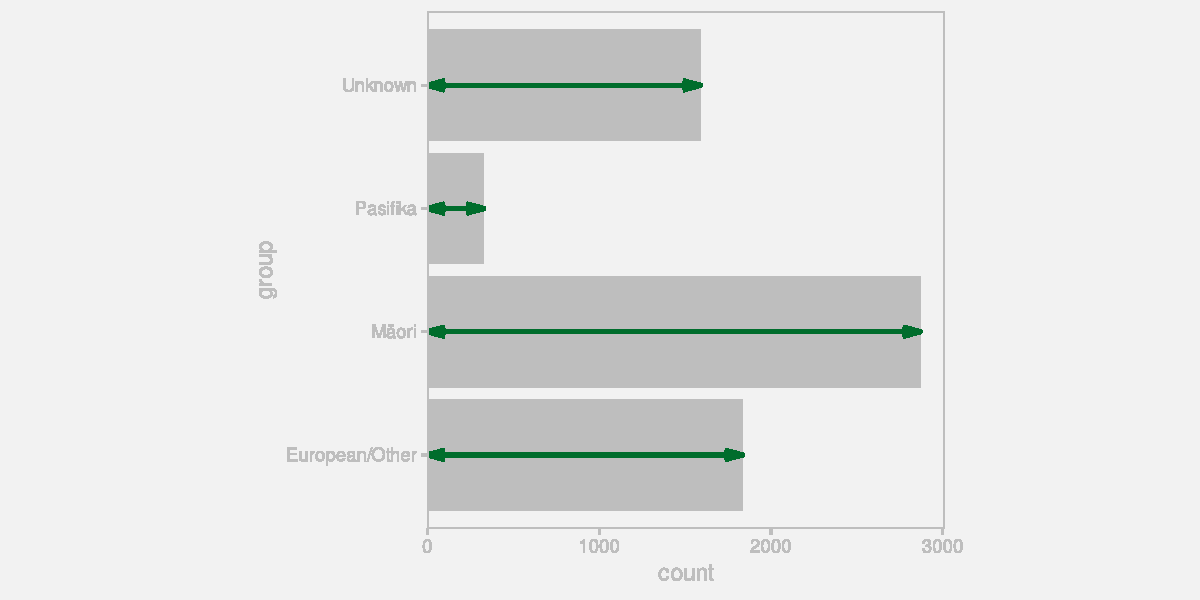
\includegraphics[width=1\linewidth,height=\textheight,keepaspectratio]{index_files/mediabag/mapping-visual-features_files/figure-pdf/fig-length-1.pdf}

}

\caption{\label{fig-length}A bar plot of number of crimes for different
ethnic groups. The data values, the total number of crimes, have been
mapped to the \textbf{lengths} of the bars (the purple lines).}

\end{figure}%

There is another mapping being used in Figure~\ref{fig-bar}: The crime
group is encoded as the vertical \textbf{positions} of the bars (see
Figure~\ref{fig-position}). Each group value is mapped to the vertical
position of one rectangle.

\begin{figure}

\centering{

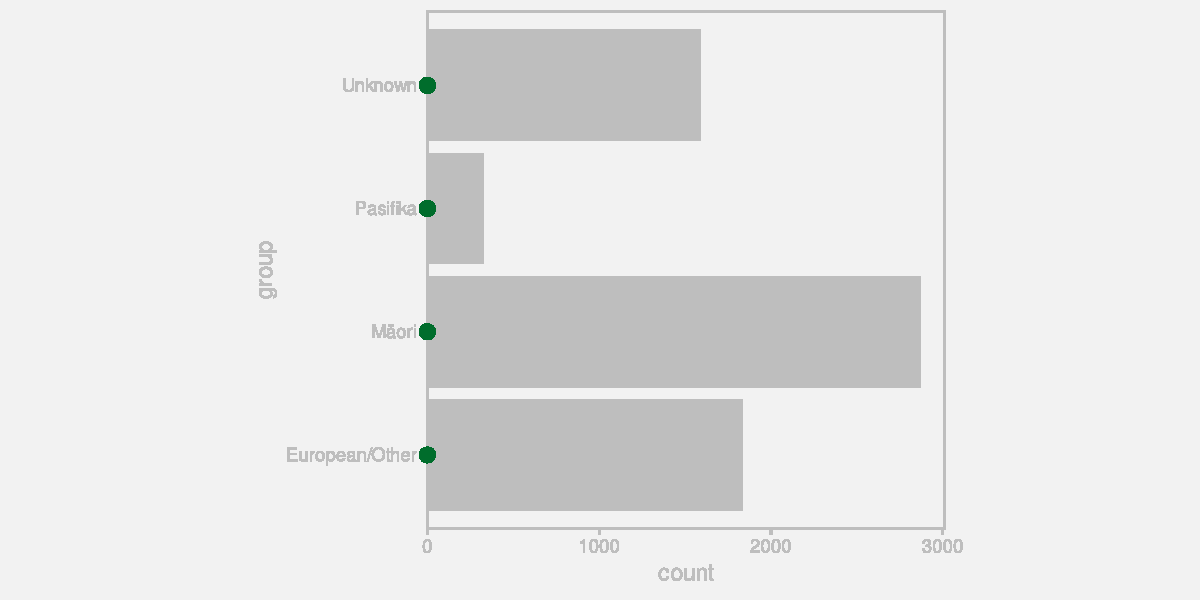
\includegraphics[width=1\linewidth,height=\textheight,keepaspectratio]{index_files/mediabag/mapping-visual-features_files/figure-pdf/fig-position-1.pdf}

}

\caption{\label{fig-position}A bar plot of number of crimes for
different ethnic groups. The data values, the ethnic groups, have been
mapped to the \textbf{positions} of the bars (the purple dots).}

\end{figure}%

\textbf{Length} and \textbf{position} are examples of basic visual
features. One way to make an effective data visualisation is to encode
data values as the basic visual features of a data symbol. This is
effective because basic visual features are identified rapidly and
without conscious effort by our visual system
(Section~\ref{sec-visual-processing}). Figure~\ref{fig-visual-features}
shows some other examples of basic visual features.\footnote{Mention
  different terminologies: visual feature vs visual channel vs visual
  dimension.

  Acknowledge that a much larger list has been considered and evaluated
  by different researchers. For example p26 of ``Better data
  visualizations'' Jonathan Schwabish. There should also be some stuff
  from research articles in DataVis/README

  Also acknowledge that there is not a one-to-one correspondence between
  visual features that are initially perceived by visual system and the
  visual channels of Cleveland and Mcgill, but it is a useful
  simplification to elide them.}

\begin{figure}

\centering{

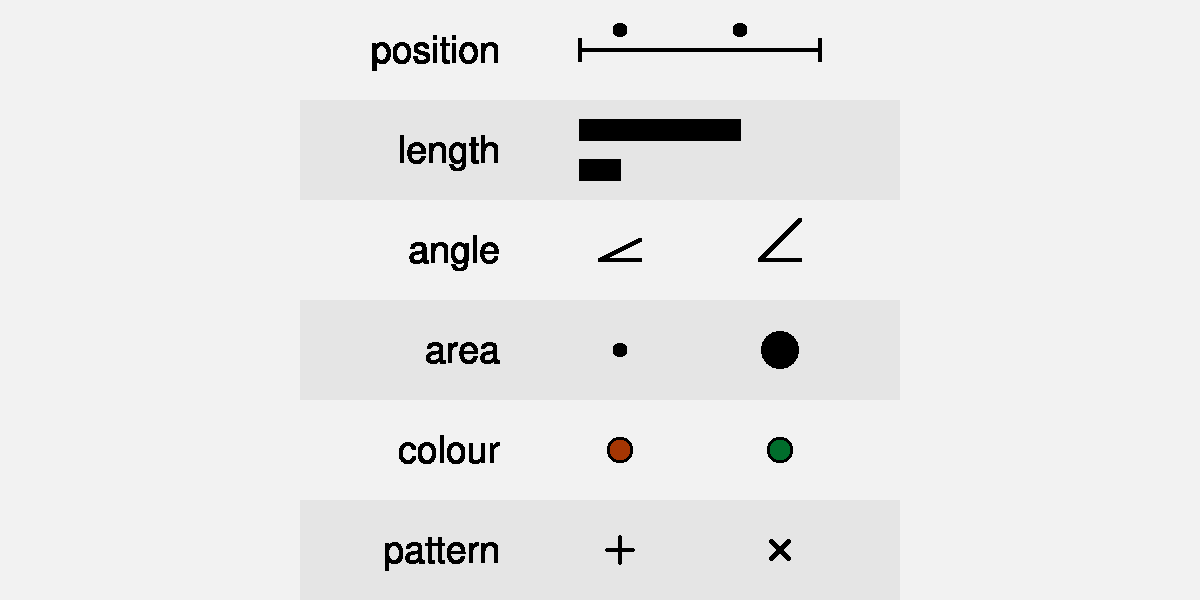
\includegraphics[width=1\linewidth,height=\textheight,keepaspectratio]{index_files/mediabag/mapping-visual-features_files/figure-pdf/fig-visual-features-1.pdf}

}

\caption[\label{fig-visual-features}Some examples of basic visual
features are \textbf{position}, \textbf{length}, \textbf{angle},
\textbf{area}, \textbf{colour}, and \textbf{shape}.]{\label{fig-visual-features}Some examples of basic visual
features are \textbf{position}, \textbf{length}, \textbf{angle},
\textbf{area}, \textbf{colour}, and \textbf{shape}.\footnotemark{}}

\end{figure}%
\footnotetext{Talk about
  this being a quite small list; munzner has more, and Wolfe and
  Horowitz 2004 suggest 20? (see Pomerantz and Cragin (2014))}

\begin{quote}
One reason why a bar plot is an effective data visualisation is because
it involves a mapping from data values to the basic visual features of
data symbols---the positions and lengths of bars---and basic visual
features are processed rapidly and subconsciously by our visual system.
\end{quote}

\section{Quantitative features}\label{sec-quant-features}

As we discussed in Chapter~\ref{sec-visual-system}, the real purpose of
encoding data values as data symbols is to make use of the visual system
to \textbf{decode} the data values from the data symbols. In this
section, we are considering mappings from data values to basic visual
features, so we need to consider how well we are able to \textbf{decode}
from \textbf{visual features} to \textbf{data values}
(Figure~\ref{fig-visual-feature-decode}).

\begin{figure}

\centering{

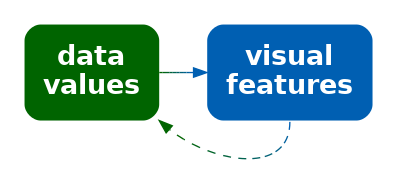
\includegraphics[scale=0.5]{Diagrams/data-vis-decode.png}

}

\caption{\label{fig-visual-feature-decode}When we encode data values as
visual features, we want to map to a visual feature that allows us to
decode the data values from the visual fearure.}

\end{figure}%

One issue to consider is whether a visual feature is able to represent
all of the information in the data values.\footnote{The idea of matching
  the type of data---nominal, ordinal, interval, or ratio---as well as
  the categorisation of visual feature types is described in Zhang
  (1996). Munzner (2014), following Mackinlay (1986), refers to this
  idea as ``expressiveness'' (vs ``effectiveness'' which is more about
  accuracy). Pinker 1990, p.~111 talks about the different types of data
  that can be extracted from different visual representations.} Some
types of data contain more information than others:

\begin{itemize}
\item
  \textbf{Quantitative} data consists of numeric values, which naturally
  possess not only an ordering, but information about the size of
  differences between values. For example, the year 2020 comes after the
  year 2010 and there is a gap of 10 years in between. This is also
  referred to as \textbf{interval} data. \textbf{Ratio} data is
  quantitative data that also contains a ``zero'' reference value, so
  there is also information about absolute size and ratios of
  differences. For example, 200 offenders is twice as many as 100
  offenders.
\item
  \textbf{Qualitative} data consists of categorical values.
  \textbf{Ordinal} data consists of categories that are ordered, but
  there is no information about the size of differences. For example, a
  ``high'' crime level is more severe than a ``medium'' crime level,
  which is more severe than a ``low'' crime level, but we cannot measure
  the size of the differences. \textbf{Nominal} data consists of just
  group labels, e.g., ethnic groups, and the only information we have is
  that the categories are different from each other.
\end{itemize}

Figure~\ref{fig-quant-features} shows that \textbf{position},
\textbf{length}, \textbf{angle}, and \textbf{area} are visual features
that are capable of representing \textbf{quantitative} data values. For
example, a bar that is twice as high as another bar comfortably
represents a data value that is twice as much as another data value. All
but \textbf{position} also possess a natural representation of zero.

\begin{figure}

\centering{

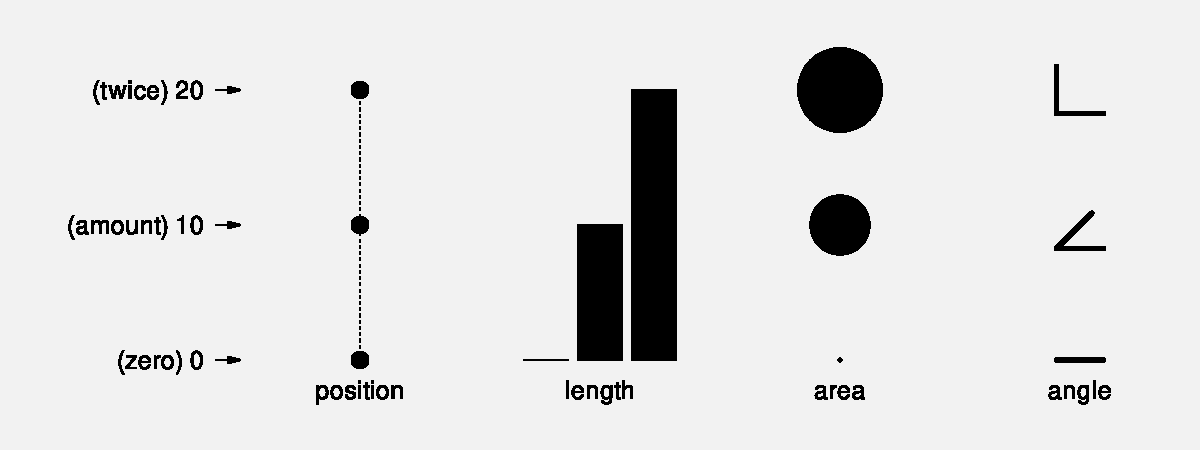
\includegraphics[width=1\linewidth,height=\textheight,keepaspectratio]{index_files/mediabag/mapping-visual-features_files/figure-pdf/fig-quant-features-1.pdf}

}

\caption{\label{fig-quant-features}The visual features position, length,
area, and angle are all appropriate visual features for visualising
quantitative data values.}

\end{figure}%

By contrast, Figure~\ref{fig-not-quant} shows that \textbf{colour} and
\textbf{shape} are \emph{not} capable of representing quantitative
values. For example, the colour blue is not twice the colour green and a
plus sign is not 10 more than a triangle. In effect, these visual
representations \emph{lose} information.

\begin{figure}

\centering{

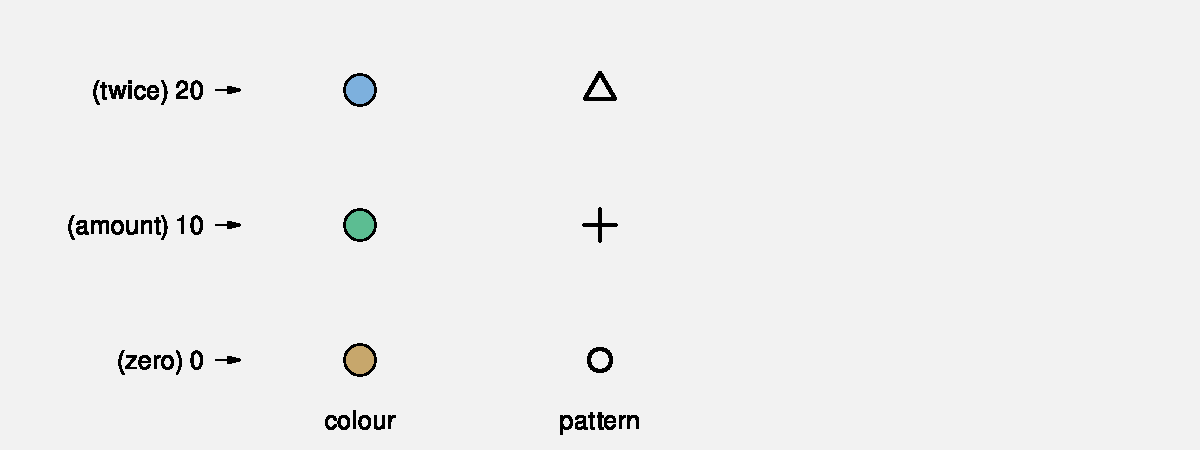
\includegraphics[width=1\linewidth,height=\textheight,keepaspectratio]{index_files/mediabag/mapping-visual-features_files/figure-pdf/fig-not-quant-1.pdf}

}

\caption{\label{fig-not-quant}The visual features \textbf{colour} and
\textbf{shape} are not capable of visualising quantitative data values.}

\end{figure}%

The bar plot in Figure~\ref{fig-bar} visualises the total number of
offenders, which are quantitative data values. These quantitative values
are encoded as the \textbf{lengths} of bars, which is a visual feature
that is capable of conveying all of the information in quantitative
values.

\begin{quote}
One reason why a bar plot is effective for visualising
\textbf{quantitative data values} is because the quantitative data
values, the counts, are mapped to a \textbf{quantitative visual
feature}, the lengths of the bars.
\end{quote}

\section{Qualitative features}\label{sec-qual-features}

If we have \textbf{qualitative} data, then we are primarily concerned
with conveying whether data values are the same or different.
Figure~\ref{fig-qual-features} shows that \textbf{position},
\textbf{colour}, and \textbf{shape} are capable of representing
qualitative data values. For example, blue is clearly different from
green, which is clearly different from brown. In
Section~\ref{sec-visual-model-groups} we saw that we also easily
identify visual objects that have the same visual features.

\begin{figure}

\centering{

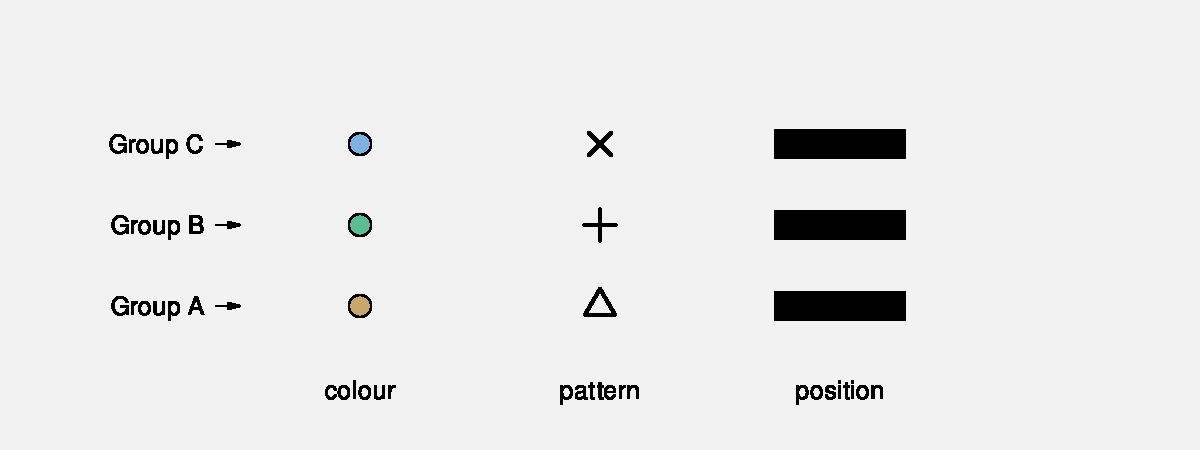
\includegraphics[width=1\linewidth,height=\textheight,keepaspectratio]{index_files/mediabag/mapping-visual-features_files/figure-pdf/fig-qual-features-1.pdf}

}

\caption{\label{fig-qual-features}The visual features \textbf{colour},
\textbf{shape}, and \textbf{position} are capable of representing
different groups.}

\end{figure}%

By contrast, Figure~\ref{fig-not-qual} shows that \textbf{length},
\textbf{area}, and \textbf{angle} are not appropriate for representing
qualitative data values. While we can identify whether lengths or areas
are different from each other, these visual features imply an inherent
\emph{order}, which is misleading because that \emph{adds} information
that is not present in the data values.

\begin{figure}

\centering{

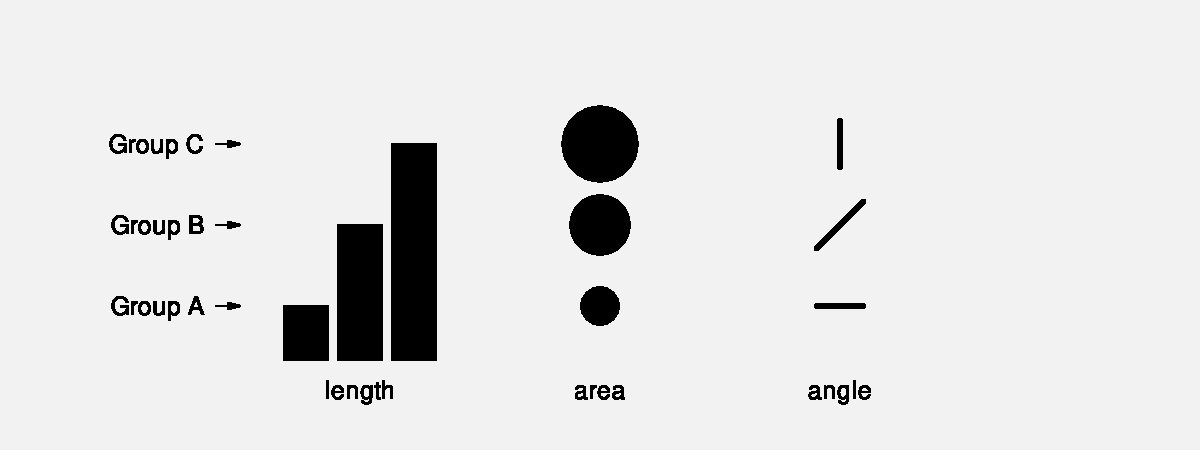
\includegraphics[width=1\linewidth,height=\textheight,keepaspectratio]{index_files/mediabag/mapping-visual-features_files/figure-pdf/fig-not-qual-1.pdf}

}

\caption{\label{fig-not-qual}The visual features \textbf{length},
\textbf{area}, and \textbf{angle} are not appropriate for representing
qualitative data values because they imply an ordering of data values
that have no inherent order.}

\end{figure}%

The bar plot in Figure~\ref{fig-bar} encodes the ethnic groups, which
are qualitative data values, as the \textbf{position} of bars, which is
a qualitative visual feature.

\begin{quote}
One reason why a bar plot is effective for visualising
\textbf{qualitative data values} is because the qualitative data values,
the groups, are mapped to a \textbf{qualitative visual feature}, the
positions of the bars.
\end{quote}

\section{Accuracy}\label{sec-accuracy}

Another issue that impacts on how well we can \textbf{decode} the data
values from a visual feature (Figure~\ref{fig-visual-feature-decode}) is
the \textbf{accuracy} with which we can perceive quantitative values
from visual features. For example, how well can we perceive the size of
the difference between the length of two bars?\footnote{The pioneering
  work on the accuracy of different visual features for statistical
  graphics was carried out by William S. Cleveland and McGill (1984).
  Their results have been replicated several times in subsequent
  studies, including Heer and Bostock (2010). The rankings were extended
  to a larger set of visual features by Mackinlay (1986), although
  somewhat only by inference from other psychophyscial results, rather
  than by direct experiment. An argument for ranking the accuracy of
  visual features can also be made from Steven's Law (Stevens 1957),
  which states that the perception of the magnitude of different stimuli
  follows a power law. For example, the perception of length has a power
  of approximately one (linear), which suggests that we accurately
  perceive the magnitude of lengths, while area has a power less than
  one, which suggests that we underestimate the magnitude of areas.}

It is easy to demonstrate that judgements of this sort are harder for
some visual features than others. For example,
Figure~\ref{fig-accuracy-demo} presents sets of three bars, which differ
by \textbf{length}, circles, which differ by \textbf{area}, and
polygons, which differ by \textbf{shape} (number of sides). Judging the
relative sizes of the bars is easier than judging the relative sizes of
the circles and comparing the polygons is extremely difficult.

\begin{figure}

\centering{

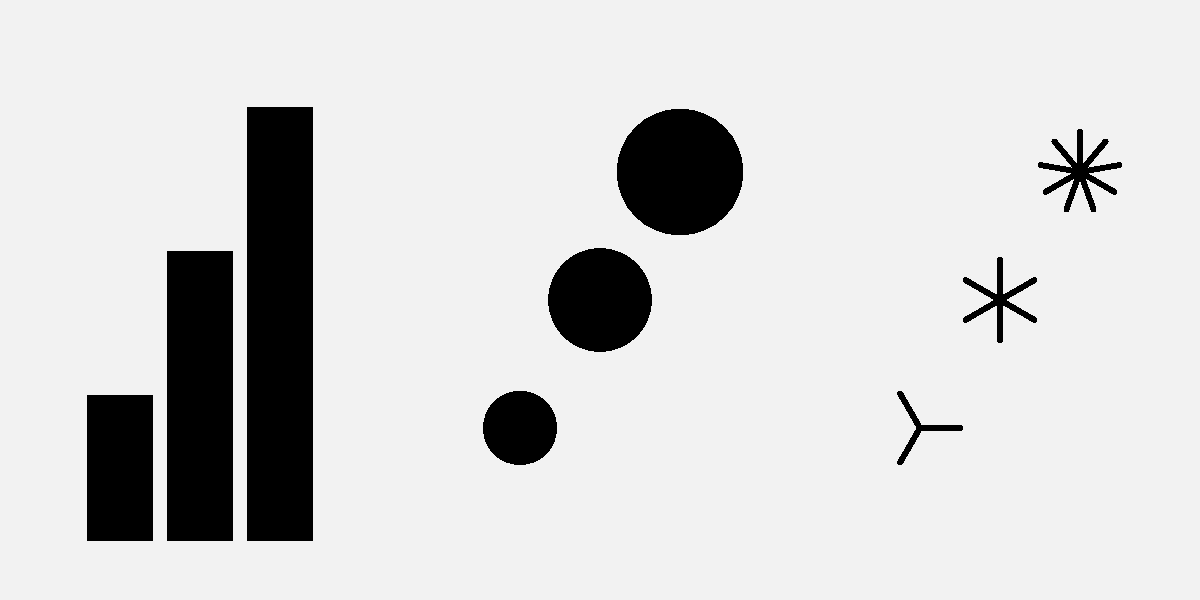
\includegraphics[width=1\linewidth,height=\textheight,keepaspectratio]{index_files/mediabag/mapping-visual-features_files/figure-pdf/fig-accuracy-demo-1.pdf}

}

\caption{\label{fig-accuracy-demo}A demonstration of differences in
accuracy between basic visual features. For each set of symbols, how
much larger (or brighter) are the larger (or brighter) symbols?}

\end{figure}%

This issue has been studied experimentally and Figure~\ref{fig-accuracy}
shows the established ordering of the accuracy of basic visual features,
with more accurate visual features at the top.\footnote{In William S.
  Cleveland and McGill (1984), comparisons of bars were treated as
  \textbf{position} judgements rather than \textbf{length} judgements,
  unless the bars were unaligned (see Section~\ref{sec-unaligned}), so
  this table is a slightly fuzzy representation of their results.
  However, the general ordering of visual features is basically
  consistent with William S. Cleveland and McGill (1984). \textbf{NEED}
  to mention that these rankings are based on perceiving part-of-whole
  (what proportion of A is B?). Cite studies that look at rankings
  relative to other tasks McColeman et al (2021) Davis et al (2022)} A
data visualisation that encodes data values as visual features near the
top of this ranking will be more effective than one that encodes data
values as visual features near the bottom.

\begin{figure}

\centering{

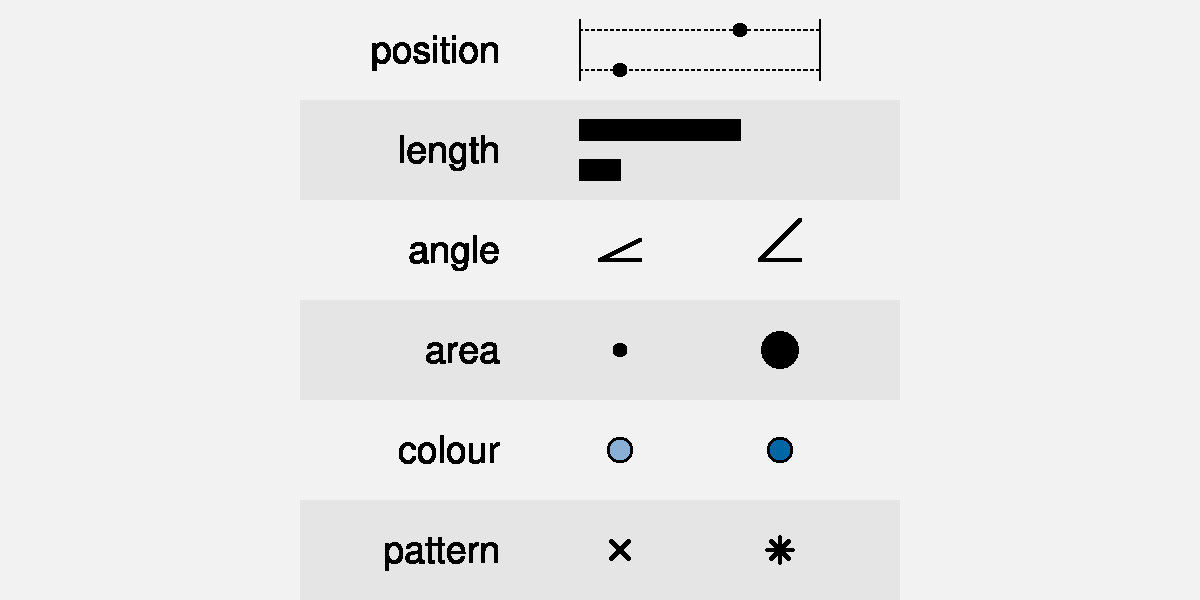
\includegraphics[width=1\linewidth,height=\textheight,keepaspectratio]{index_files/mediabag/mapping-visual-features_files/figure-pdf/fig-accuracy-1.pdf}

}

\caption{\label{fig-accuracy}An ordering of basic visual features in
terms of their accuracy, with more accurate at the top.}

\end{figure}%

The bar plot in Figure~\ref{fig-bar} encodes the total number of
offenders, which are quantitative values, as the \textbf{lengths} of
bars, which is an \textbf{accurate} visual feature. This means that
viewers can make accurate comparisons between the lengths of the bars.

\begin{quote}
One reason why a bar plot is effective for visualising
\textbf{quantitative data values} is because the quantitative data
values, counts or proportions, are encoded as a very \textbf{accurate
visual feature}, the lengths of the bars.
\end{quote}

\section{Capacity}\label{sec-capacity}

When we are visualising \textbf{qualitative} data values, we are no
longer concerned with accurately perceiving the size of differences; all
we are concerned with is perceiving whether two values are different.
For example, can we perceive a difference between two colours?

The issue in this scenario is the \textbf{capacity} of a visual feature:
how many different categories can be represented (and still perceived as
clearly different from each other).

Figure~\ref{fig-colour-cap} shows that \textbf{colour} has a limited
capacity. A small number of different colours are very easy to
differentiate, but the differences become harder to perceive with a
greater number of colours.\footnote{``Do not use more than 10 colors for
  coding symbols if reliable identification is required, especially if
  the symbols are to be used against a variety of backgrounds.'' Ware
  4th ed {[}G4.18{]} p 126. Also cite the study that shows how capacity
  depends on whether points are spread out or arranged regularly ?}

\begin{figure}

\centering{

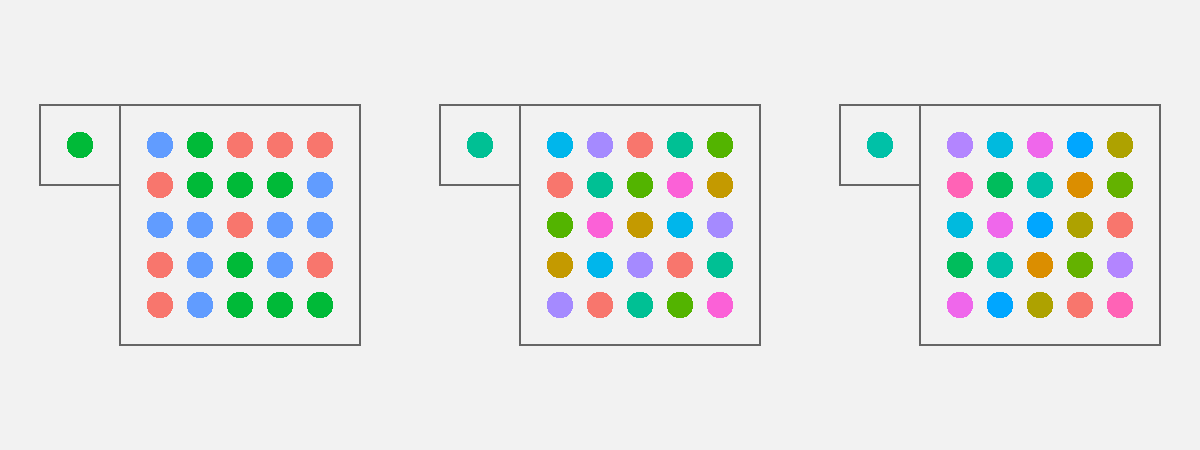
\includegraphics[width=1\linewidth,height=\textheight,keepaspectratio]{index_files/mediabag/mapping-visual-features_files/figure-pdf/fig-colour-cap-1.pdf}

}

\caption{\label{fig-colour-cap}Mapping qualitative data values to colour
works well for a small number of colours, but less well for a large
number of colours. It is quite easy to distinguish between the three
colours on the left and even between the seven colours in the middle,
but it becomes harder for the eleven colours on the right.}

\end{figure}%

By contrast, Figure~\ref{fig-pos-cap} shows that \textbf{position} has a
very large capacity. We can easily differentiate between locations even
as the number of locations becomes large.

\begin{figure}

\centering{

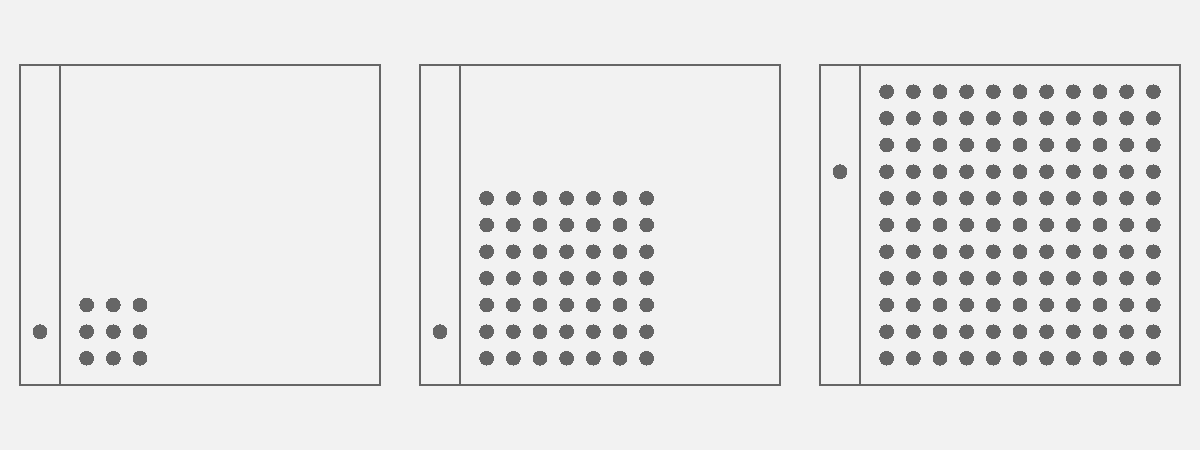
\includegraphics[width=1\linewidth,height=\textheight,keepaspectratio]{index_files/mediabag/mapping-visual-features_files/figure-pdf/fig-pos-cap-1.pdf}

}

\caption{\label{fig-pos-cap}Mapping qualitative data values to position
works well for both a small number of positions and for a large number
of positions.}

\end{figure}%

The bar plot in Figure~\ref{fig-bar} encodes the ethnic group as the
\textbf{position} of bars, which makes it easy to differentiate between
the different ethnic groups.

\begin{quote}
One reason why a bar plot is effective for visualising
\textbf{qualitative data values} is because the qualitative data values,
the groups, are encoded as a visual feature that has excellent
\textbf{capacity}, the positions of the bars.
\end{quote}

\textbf{Need} to also mention limited capacity of point shapes?
Footnote: ``Evaluation of symbol contrast in scatterplots'' Li et al
(2009). Cleveland ``The Elements of Graphing Data'' 1994 {[}p239{]}
suggests set of discriminable data point shapes: o, +, \textless, s, w,
which is small, though no explicit mention of capacity limit.)

\section{Case study: Dot plots}\label{sec-dot-plots}

We have seen that, for several reasons, Figure~\ref{fig-bar} is an
effective way to visualise the total number of offenders for different
ethnic groups. Figure~\ref{fig-dot} shows an alternative representation
of these data in the form of a dot plot (William S. Cleveland 1985a).

\begin{figure}

\centering{

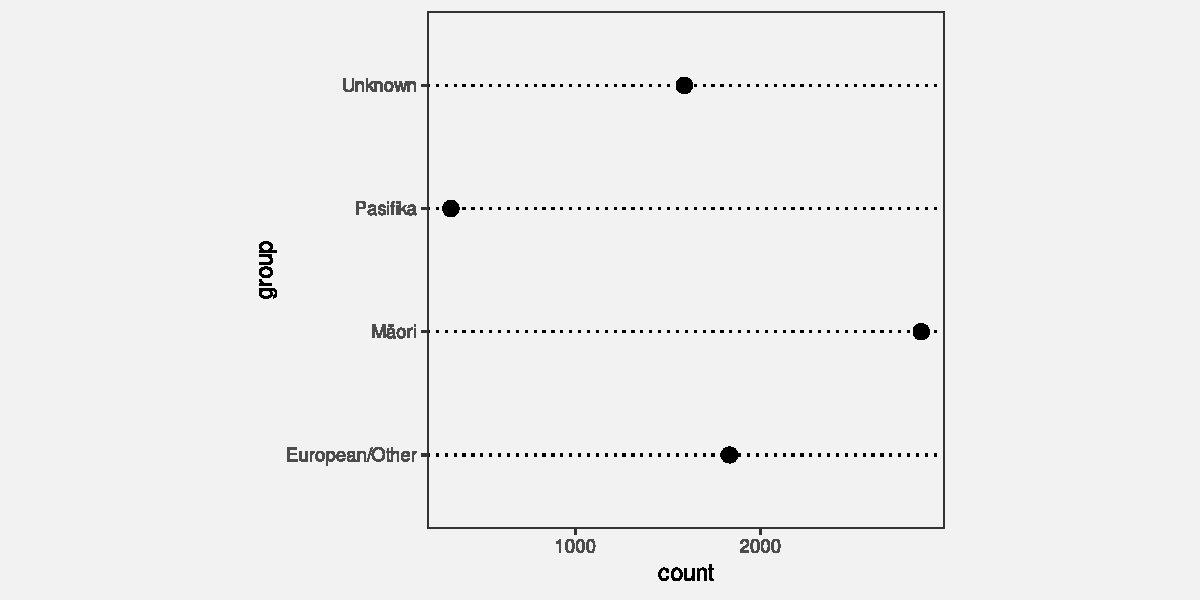
\includegraphics[width=1\linewidth,height=\textheight,keepaspectratio]{index_files/mediabag/mapping-visual-features_files/figure-pdf/fig-dot-1.pdf}

}

\caption{\label{fig-dot}A dot plot of the number of crimes for different
ethnic groups. The data symbols in this plot are the data points.}

\end{figure}%

Like the bar plot, this is a very effective data visualisation, and for
very similar reasons. This data visualisation uses a different data
symbol, data points instead of bars, but each data value is encoded as
the basic visual feature of one data symbol. Furthermore, the
quantitative data values (the totals) are encoded as the horizontal
\textbf{position} of the points, which is a visual feature that is
capable of representing numeric values and it is a very accurate visual
feature, and the qualitative data values (the groups) are encoded as the
vertical \textbf{position} of the points, which is a visual feature with
a high capacity.

It could be argued that the dot plot in Figure~\ref{fig-dot} is even
\emph{more} effective than the bar plot in Figure~\ref{fig-bar} for
perceiving the differences between totals because \textbf{position}
ranks higher than \textbf{length} in Figure~\ref{fig-accuracy}. On the
other hand, if we want to compare totals in terms of their ratios,
Figure~\ref{fig-bar} is superior because it includes a representation of
zero.

\section{Case study: Pie charts}\label{case-study-pie-charts}

Figure~\ref{fig-pie} shows yet another visualisation of the total number
of offenders for different ethnic groups, this time a pie chart. This is
a less effective representation of the data than the bar plot in
Figure~\ref{fig-bar} or the dot plot in Figure~\ref{fig-dot} and we can
use familiar reasoning to see why.

\begin{figure}

\centering{

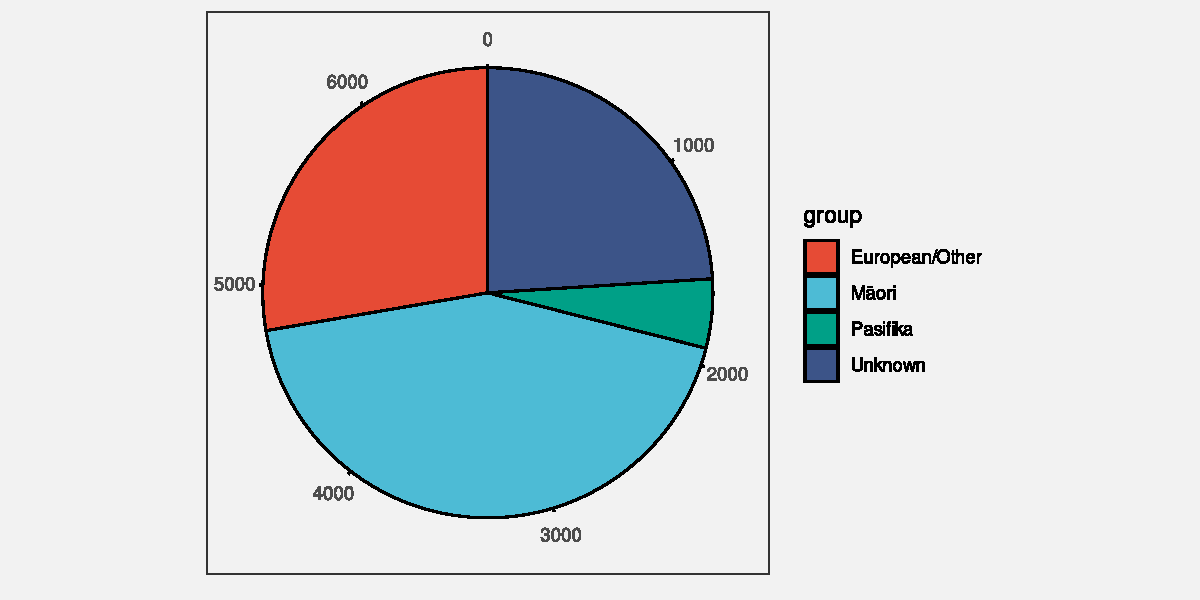
\includegraphics[width=1\linewidth,height=\textheight,keepaspectratio]{index_files/mediabag/mapping-visual-features_files/figure-pdf/fig-pie-1.pdf}

}

\caption{\label{fig-pie}A pie chart of the number of crimes for
different ethnic groups. The data symbols in this plot are the pie
wedges.}

\end{figure}%

The data symbols in Figure~\ref{fig-pie} are wedges or segments of a
circle and, on the positive side, the data values are encoded as basic
visual features of these symbols: The total values are encoded as the
\textbf{angle} and/or \textbf{area} of the wedges and the group values
are encoded as the \textbf{colour} of the wedges.\footnote{cite the
  paper that looked at people decoding from area vs angle vs chord(!) vs
  arc length(!) for pie charts ``The relative merits of circles and bars
  for representing component parts.'' Eells (1926)} Although
\textbf{colour} is an appropriate visual feature to represent
\textbf{qualitative} data, and it has sufficient capacity to
differentiate between only four groups, the encoding of quantitative
values as \textbf{angle} and/or \textbf{area} leads to less accurate
perception of the differences between totals (compared to the lengths
and positions encodings that were employed in the bar plot and the dot
plot).

\section{Summary}\label{summary-2}

A bar plot is a very common data visualisation for representing numeric
values, particularly counts, for several different groups. There are
several reasons why bar plots work so well:

\begin{itemize}
\tightlist
\item
  A bar plot encodes data values as basic visual features, which are
  perceived rapidly and without conscious effort.
\item
  A bar plot encodes the quantitative counts as a quantitative visual
  feature (length) and the qualitative groups as a qualitative visual
  feature (position).
\item
  A bar plot encodes the counts to a visual feature that is perceived
  very accurately (length) and the groups to a visual feature that has a
  high capacity (position).
\end{itemize}

Dot plots are also very effective for the same scenario for the same
reasons, except that a dot plot uses \textbf{position} instead of length
to represent the quantitative values.

Pie charts by comparison have some weaknesses:

\begin{itemize}
\tightlist
\item
  A pie chart encodes quantitative counts as \textbf{angle} and/or
  \textbf{area}, which is less accurate.
\item
  A pie chart encodes qualitative groups as \textbf{colour}, which has a
  lower capacity.
\end{itemize}

\begin{center}\rule{0.5\linewidth}{0.5pt}\end{center}

\theendnotes

\bookmarksetup{startatroot}

\chapter{Position}\label{sec-position}

Position is fundamental to our perception of an image.\footnote{``Design
  for Information : An Introduction to the Histories, Theories, and Best
  Practices Behind Effective Information Visualizations'' Isabel
  Meirelles (2013) ``We process spatial properties (position and size)
  separately from object properties (such as shape, color, texture,
  etc). Furthermore, position in space and time has a dominant role in
  perceptual organization, as well as in memory.'' Ware (2004, 2008),
  Card et al.~(1999), MacEachren (2004), Kosslyn (1994).

  ``How Maps Work - Representation, Visualization, and Design''
  MACEACHREN A. M. (1995) quotes Kubovy (1981) who includes position as
  one of the ``indispensable attributes''

  ``UNDERSTANDING GRAPHS AND TABLES'' Wainer (1992) quotes Arthur H.
  Robinson and Barbara Bartz Petchenik (1976) who said, ``There is
  fairly widespread philosophical agreement, which certainly accords
  with commonsense, that the spatial aspects of all existence are
  fundamental. Before an awareness of time, there is an awareness of
  relations in space.'' They conclude their book with the observation
  that ``the concept of spatial relatedness \ldots{} is a quality
  without which it is difficult or impossible for the human mind to
  apprehend anything.''}

\textbf{NOTE} that this is going to have to stick to simple
demonstrations using bar plots (e.g., stacked vs dodged). Don't get
scatter plots until chapter 10 (!) Case study q-q plots in combine.Rmd.
Ditto log-log plot.

\section{Position is relative}\label{position-is-relative}

Accuracy is really ratios not absolute values

\section{Aligned versus unaligned}\label{sec-unaligned-pos}

Elaborate on the classic order to allow for aligned vs unaligned. Not
entirely sure how to demo this with actual plot, though in quantitative
(length) there is an abstract demo.

\begin{figure}

\centering{

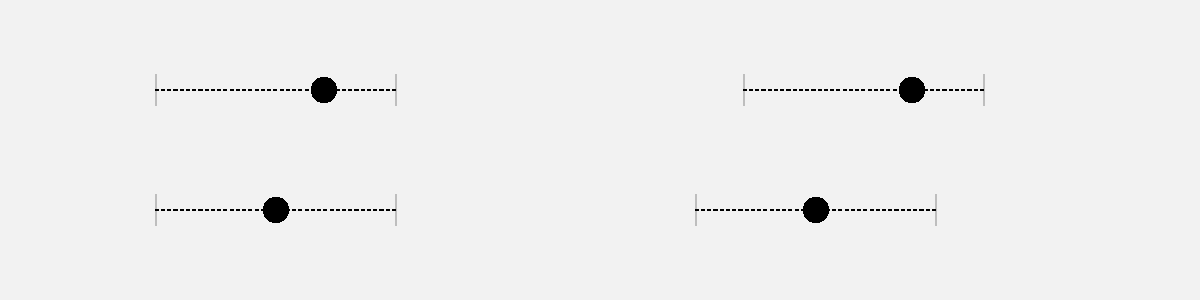
\includegraphics[width=1\linewidth,height=\textheight,keepaspectratio]{index_files/mediabag/position_files/figure-pdf/fig-unaligned-pos-1.pdf}

}

\caption{\label{fig-unaligned-pos}It is easier to compare two positions
on the left because they are \textbf{aligned}; they share a common
baseline. The two positions on the right are harder to compare because
they are \textbf{unaligned}.}

\end{figure}%

\section{Overplotting}\label{overplotting}

If a data value is mapped to a representation that is not visible,
decoding is going to be a challenge.

Refer back to Section~\ref{sec-eye}

Bring jittering case study back here. Add link from birthday cake
example back to jittering.

big data (or even medium data) - need better name =\textgreater{}
overlapping and summary plots like boxplots (then violin plots)

\section{Non-linear scales}\label{sec-non-linear}

The effective decoding of position is dependent on a linear
encoding.\footnote{Tufte, E. R. (1983). The Visual Display of
  Quantitative Information. (Tufte also emphasized a similar principle:
  ``The representation of numbers should be directly proportional to the
  quantities represented.'')}

In a non-linear encoding, the same visual difference does not decode to
the same data difference. That is going to be confusing!\footnote{Proportional
  Ink and Logarithmic Scales
  https://callingbullshit.org/tools/logarithmic\_scales.html If you plot
  log values, then the ink is proportional, but the numbers are harder
  to interpret (in my terms, you can only map back to log values)}

NOTE that there ARE some situations where non-linear position. scales
are ok, e.g., log-log. Length is still dodgy. You DO still get ordinal
info, even if cannot decode sizes of differences. Non-linearity might
actually be ok on non-position scales, e.g., a colour scale for numeric
data, where differences are smaller at one end; all you are after, if
you are using colour, is ordinal, so changing colours more swiftly at
one end of the scale is ok (?) At least some `colorspace' functions
allow non-linear palettes. Revisit in qualitative.Rmd to point out that
non-linear ordinal scales are ok, e.g., jet colour scale

Nice example of log-log scales in The Signal and the Noise (Nate Silver)
See 787resources/Examples/2025-08-signal-noise-log-log

Log log scales a good example of asking what is it you want to see? You
cannot extract raw data or a compare raw data points. But all you want
is to see the data summary of correlation so no harm no foul.

\section{Summary}\label{summary-3}

\begin{center}\rule{0.5\linewidth}{0.5pt}\end{center}

\theendnotes

\bookmarksetup{startatroot}

\chapter{Length}\label{sec-quantitative}

Figure~\ref{fig-bar-district} shows a bar plot of the total number of
offenders in each police district in New Zealand (for ages 14 to 16 and
from 2011 to 2021). For the reasons outlined in
Chapter~\ref{sec-mapping-visual-features}, this data visualisation is
effective for comparing the number of offenders in different police
districts.

\begin{figure}

\centering{

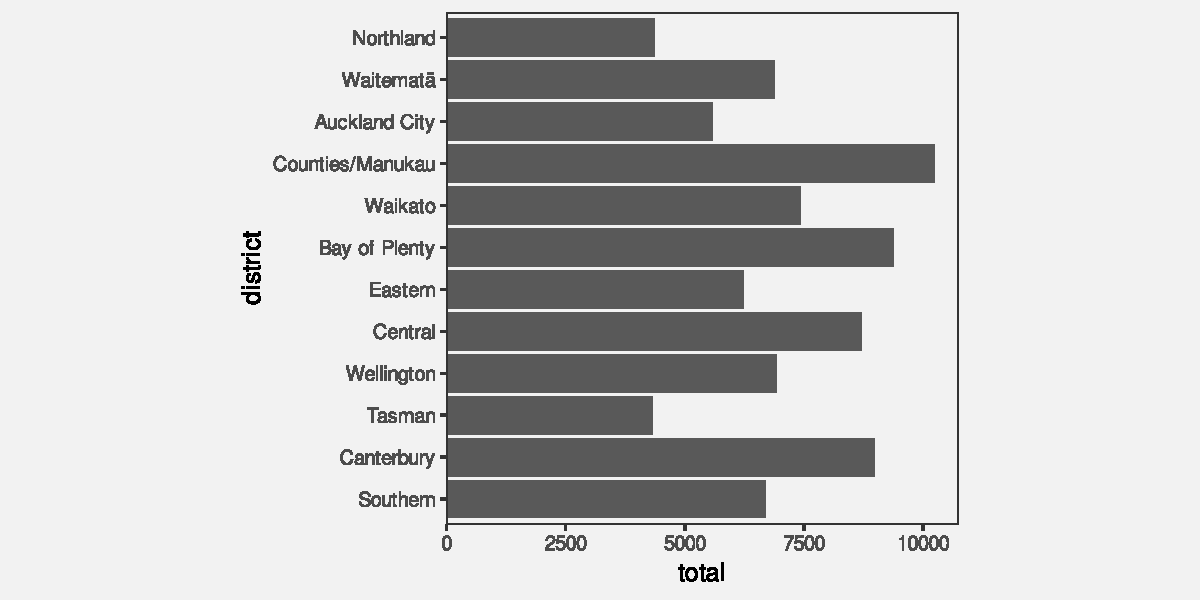
\includegraphics[width=1\linewidth,height=\textheight,keepaspectratio]{index_files/mediabag/quantitative_files/figure-pdf/fig-bar-district-1.pdf}

}

\caption{\label{fig-bar-district}A bar plot of the number of offenders
for different police districts, with the districts ordered from North to
South.}

\end{figure}%

Figure~\ref{fig-bar-district-ordered} shows a bar plot of the same data,
but with the bars ordered from longest to shortest. This data
visualisation uses the same mappings as
Figure~\ref{fig-bar-district}---police districts are encoded as the
vertical positions of the bars and the total counts are encoded as the
lengths of the bars---which means that it is also effective for
comparing the total number of offenders between police districts.

\begin{figure}

\centering{

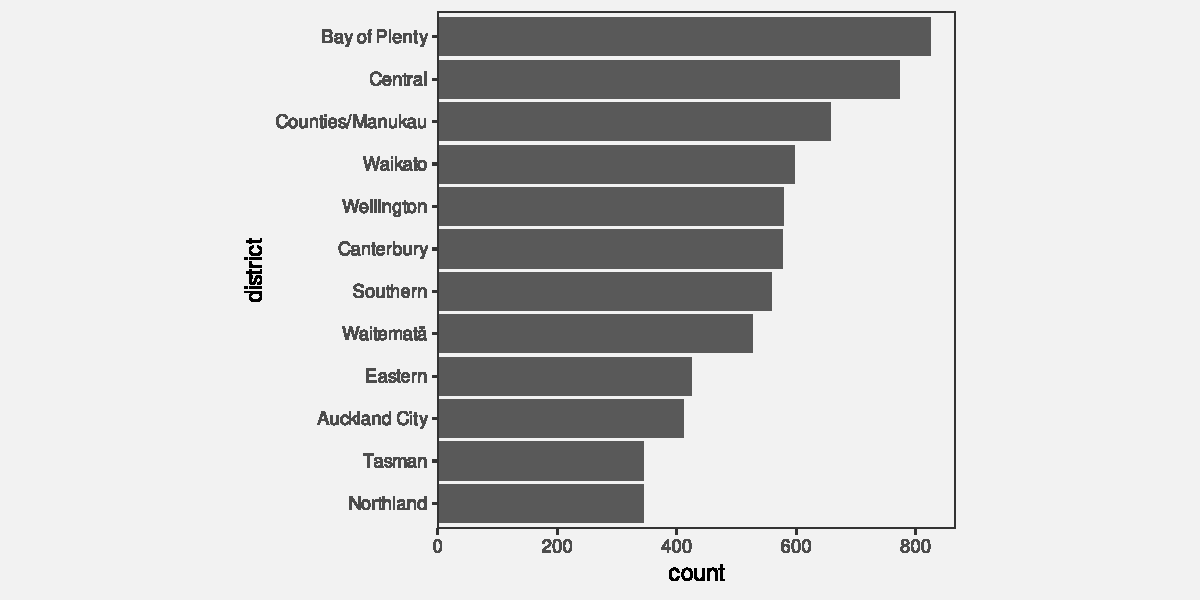
\includegraphics[width=1\linewidth,height=\textheight,keepaspectratio]{index_files/mediabag/quantitative_files/figure-pdf/fig-bar-district-ordered-1.pdf}

}

\caption{\label{fig-bar-district-ordered}A bar plot of the number of
offenders for different police districts, with the districts ordered
from largest number of offenders to smallest.}

\end{figure}%

However, Figure~\ref{fig-bar-district-ordered} is \emph{more} effective
than Figure~\ref{fig-bar-district} for some comparisons. For example, it
is easier to compare the Northland district with the Tasman district in
Figure~\ref{fig-bar-district-ordered}. The fact that two data
visualisations with the same mappings can have a different effectiveness
suggests that there is more to know about how different visual features
work.

This section covers some more details about how the \textbf{length}
visual feature works.

\section{The distance effect}\label{sec-distance-effect}

In Section~\ref{sec-accuracy}, we saw that \textbf{position} and
\textbf{length} were the most accurate visual features (see
Figure~\ref{fig-accuracy}). However, this accuracy decreases if the two
visual features that are being compared are not in close proximity (see
Figure~\ref{fig-distance-effect}).\footnote{The first demonstration of
  the ``distance effect'' is attributed to William S. Cleveland and
  McGill (1984). It has since been replicated several times, for
  example, by Talbot et al. (2014).}

This helps to explain why Figure~\ref{fig-bar-district-ordered} is more
effective than Figure~\ref{fig-bar-district} for some comparisons (e.g.,
Northland versus Tasman).

\begin{figure}

\centering{

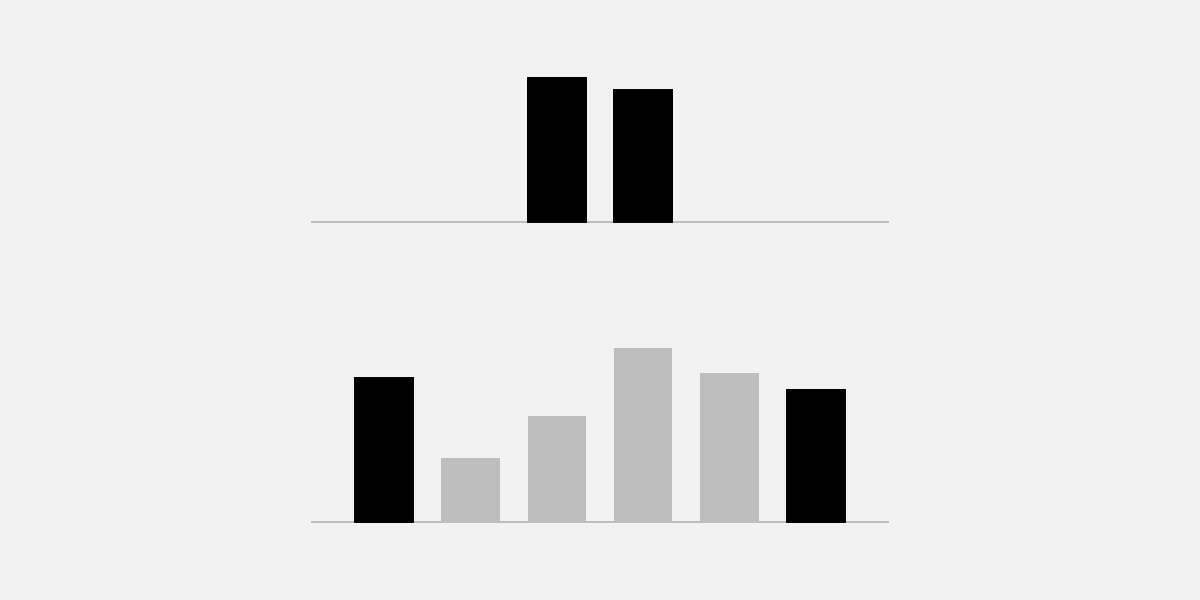
\includegraphics[width=1\linewidth,height=\textheight,keepaspectratio]{index_files/mediabag/quantitative_files/figure-pdf/fig-distance-effect-1.pdf}

}

\caption{\label{fig-distance-effect}Two bars are easier to compare if
they are close to each other (top row). If there is a distance between
the bars and/or there are distractors (other bars) in between then
comparisons are less accurate (bottom row). On both the top and bottom
row, the black bar on the left is slightly higher than the black bar on
the right.}

\end{figure}%

\begin{quote}
One reason for ordering the bars in a bar plot from longest to shortest
is because, for some common comparisons, the ordering places the bars
that are being compared closer together, which improves the accuracy of
the comparison.
\end{quote}

\section{Unaligned length}\label{sec-unaligned}

Figure~\ref{fig-unaligned-length} shows that it is harder to accurately
compare the \textbf{lengths} of two bars if they are \textbf{unaligned}
and do not share a common baseline (similar to the accuracy of comparing
\textbf{positions}; Section~\ref{sec-unaligned-pos}).

\begin{figure}

\centering{


\includegraphics[width=1\linewidth,height=\textheight,keepaspectratio]{index_files/mediabag/quantitative_files/figure-pdf/fig-unaligned-length-1.pdf}

}

\caption{\label{fig-unaligned-length}It is easier to compare the lengths
of the two bars on the left because they are \textbf{aligned}; they
share a common base. The two bars on the right are harder to compare
because they are \textbf{unaligned}.}

\end{figure}%

Figure~\ref{fig-stacked-bar} shows an alternative visualisation of the
data on the total number of offenders in different ethnic groups. The
bar plot of these data that we saw in Figure~\ref{fig-bar} encoded
ethnic groups as the \textbf{positions} of the bars so that the bars
were arranged vertically with a common left-hand edge. In
Figure~\ref{fig-stacked-bar}, the ethnic groups are encoded as different
\textbf{colours} and the bars are ``stacked'' horizontally.\footnote{In
  a stacked bar plot, groups are encoded as the positions of the bars
  and counts are encoded as the lengths of the bars, but the positions
  are in the same dimension as the lengths (in this case, both position
  and length are horizontal). In a side-by-side bar plot, the position
  of the bars is in the opposite dimension to the lengths of the bars.}

Although the total number of offenders has been encoded as the same
visual feature in both Figure~\ref{fig-stacked-bar} and
Figure~\ref{fig-bar}, the \textbf{lengths} of the bars, comparing those
lengths is much harder in Figure~\ref{fig-stacked-bar} because the
lengths are \textbf{unaligned}.

\begin{figure}

\centering{

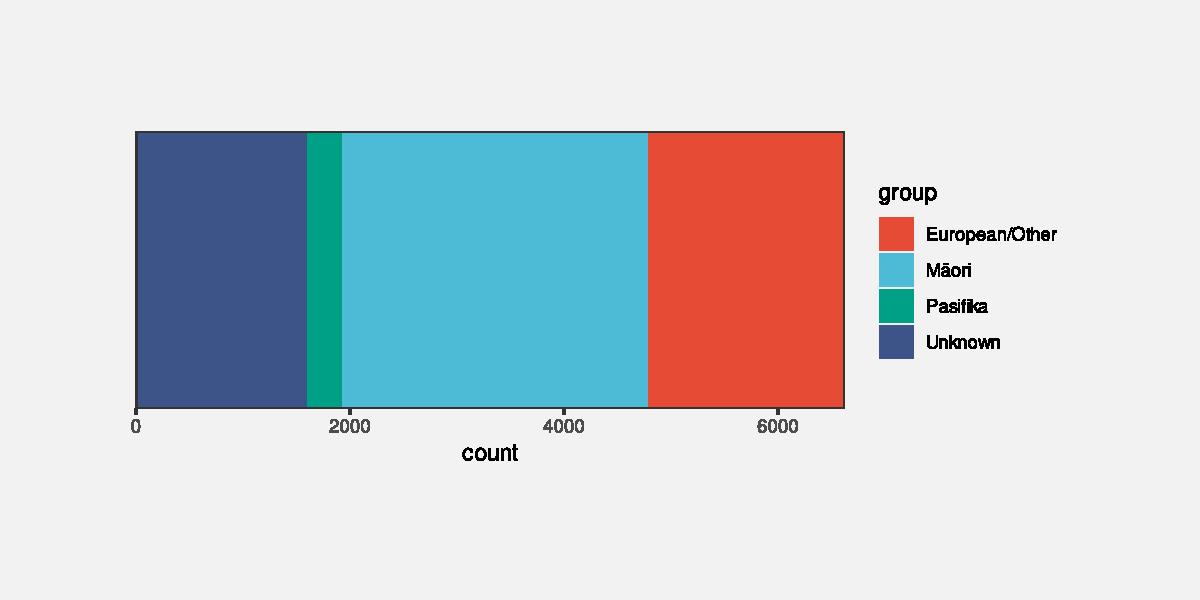
\includegraphics[width=1\linewidth,height=\textheight,keepaspectratio]{index_files/mediabag/quantitative_files/figure-pdf/fig-stacked-bar-1.pdf}

}

\caption{\label{fig-stacked-bar}A stacked bar plot of the total number
of offenders in each ethnic group.}

\end{figure}%

\begin{quote}
One reason why stacked bar plots are less effective for some comparisons
is because we are forced to compare the unaligned lengths of the bars.
\end{quote}

\section{Case study: Stacked versus side-by-side bar
plots}\label{sec-stacked-vs-side}

Stacking bars, which creates unaligned lengths, is something that arises
when we use a bar plot to show a quantitative variable broken down by
more than one qualitative variable. For example,
Table~\ref{tbl-crime-group-year} shows data on the number of offenders
in different ethnic groups for individual years (from 2011 to 2021).
This is a more detailed version of the data from
Table~\ref{tbl-crime-group-total}.

\begin{longtable}[]{@{}llrr@{}}

\caption{\label{tbl-crime-group-year}A table of the number of offenders
per year aged 14 to 16 for different ethnic groups from 2011 to 2021.
There are 44 rows of data, but just the first 6 rows are shown here.}

\tabularnewline

\toprule\noalign{}
& group & count & year \\
\midrule\noalign{}
\endhead
\bottomrule\noalign{}
\endlastfoot
1 & Māori & 5957 & 2011 \\
2 & Pasifika & 1092 & 2011 \\
3 & European/Other & 5775 & 2011 \\
4 & Unknown & 194 & 2011 \\
6 & Māori & 5458 & 2012 \\
7 & Pasifika & 1040 & 2012 \\

\end{longtable}

Figure~\ref{fig-stacked-bar-year} shows the number of offenders
(quantitative) for each ethnic group (qualitative) and for each year
from 2011 to 2021 (treated here as qualitative, or at least discrete).
In this data visualisation, the number of offenders is mapped to the
lengths of the bars, the years are mapped to the horizontal
\textbf{position} of the bars, the ethnic groups are mapped to the
colours of the bars, and the bars are stacked vertically.

The problem that we face in this situation is that there are four bars
to show for each year. Stacking the bars is one solution, but as we have
just seen, this makes some comparisons more difficult. For example, we
can easily see that the number of offenders in the unknown group
increased after 2016, but it is much harder to see what has happened to
the European/Other group since 2016.

\begin{figure}

\centering{

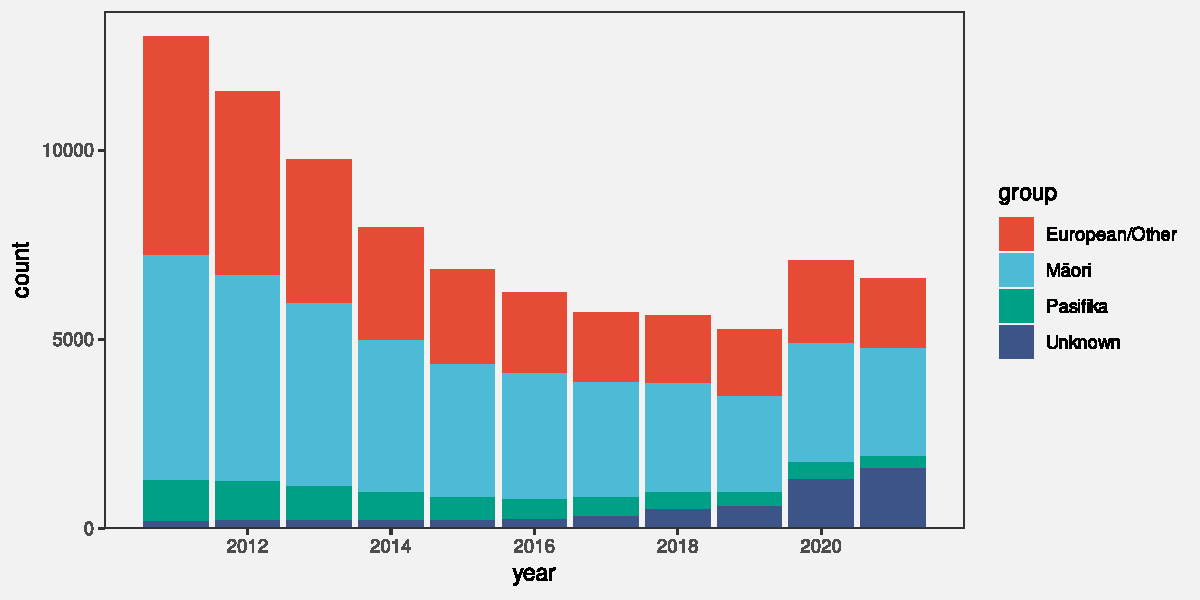
\includegraphics[width=1\linewidth,height=\textheight,keepaspectratio]{index_files/mediabag/quantitative_files/figure-pdf/fig-stacked-bar-year-1.pdf}

}

\caption{\label{fig-stacked-bar-year}A stacked bar plot of the number of
offenders in each ethnic group for each year from 2011 to 2021.}

\end{figure}%

An alternative visualisation is shown in Figure~\ref{fig-side-bar-year}.
This has placed the four ethnic groups side-by-side for each year. It is
now easier to see the changes over time for the European/Other group
because all bars are now aligned. Unfortunately, as we saw in
Section~\ref{sec-distance-effect}, some comparisons are more difficult
because the bars are now further apart and have distractors in between.

\begin{figure}

\centering{

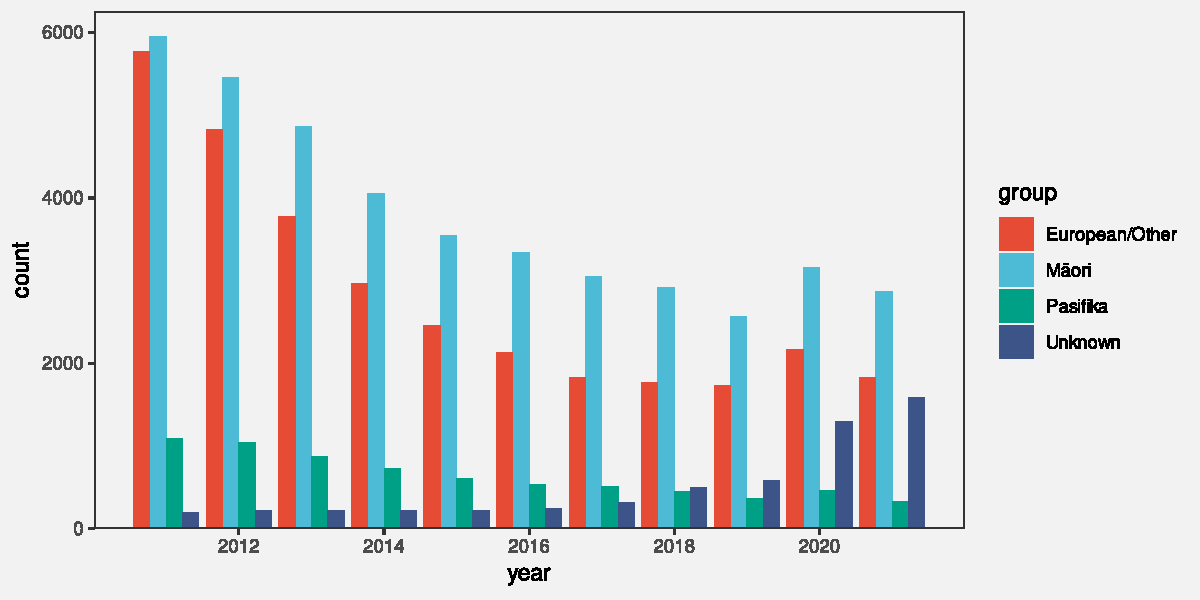
\includegraphics[width=1\linewidth,height=\textheight,keepaspectratio]{index_files/mediabag/quantitative_files/figure-pdf/fig-side-bar-year-1.pdf}

}

\caption{\label{fig-side-bar-year}A side-by-side bar plot of the number
of offenders in each ethnic group for each year from 2011 to 2021.}

\end{figure}%

Yet another variation is shown in Figure~\ref{fig-side-bar-group}. This
time we have placed all years side-by-side for each ethnic group. This
provides the clearest view of the changes over time for each ethnic
group because the relevant bars are close together and aligned. However,
there are other comparisons that are considerably more difficult because
of the distance between the relevant bars, for example, comparing
between ethnicities for a specific year.

\begin{figure}

\centering{

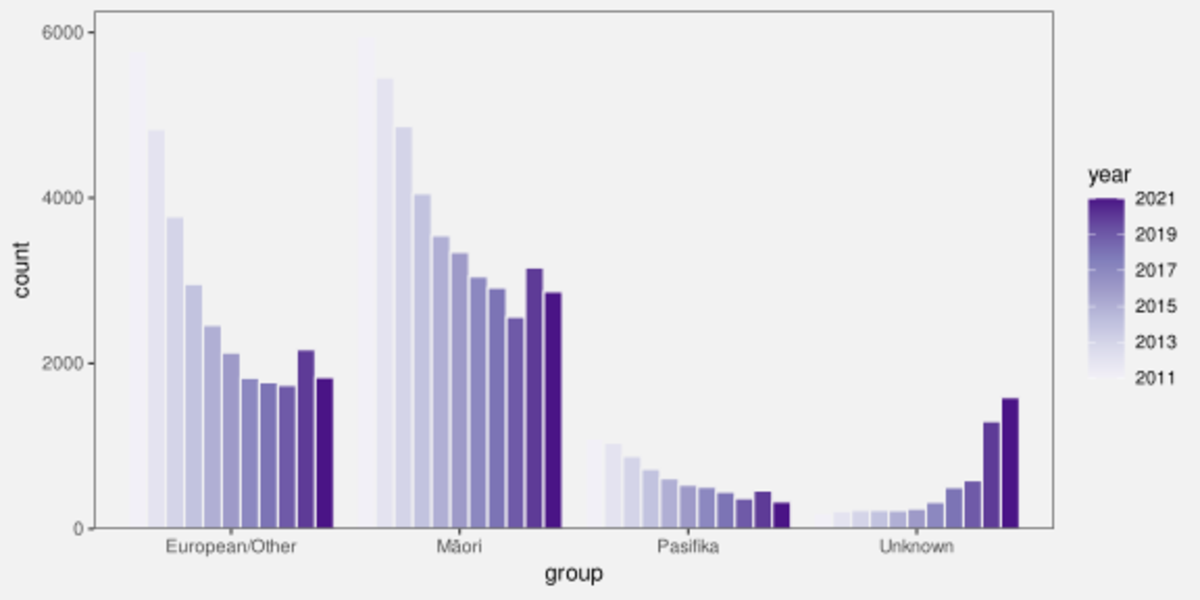
\includegraphics[width=1\linewidth,height=\textheight,keepaspectratio]{index_files/mediabag/quantitative_files/figure-pdf/fig-side-bar-group-1.pdf}

}

\caption{\label{fig-side-bar-group}A side-by-side bar plot of the number
of offenders in each ethnic group for each year from 2011 to 2021.}

\end{figure}%

There is no single best visualisation in general for this situation
because different visualisations each have their strengths and
weaknesses. If a particular sort of comparison is to be emphasised, then
one data visualisation might stand out, but there is also the option of
providing more than one data visualisation in order to cover more
comparisons.

\section{Perception is relative}\label{sec-perception-relative}

Figure~\ref{fig-relative} shows that the perception of differences
between the lengths of bars is relative; it is easier to detect smaller
differences when the visual features that we are comparing are
smaller.\footnote{The idea of perception of differences being relative
  is a very old result from Psychology known as Weber's Law (Weber 1846;
  Boring 1942).} It is easier to see that the pair of bars on the left
have different lengths and harder to see that the pair of bars on the
right have different lengths. All three pairs of bars have different
lengths, but the absolute size of the difference is the same, so the
size of the difference relative to the bar lengths gets smaller as the
bars get longer.

\begin{figure}

\centering{

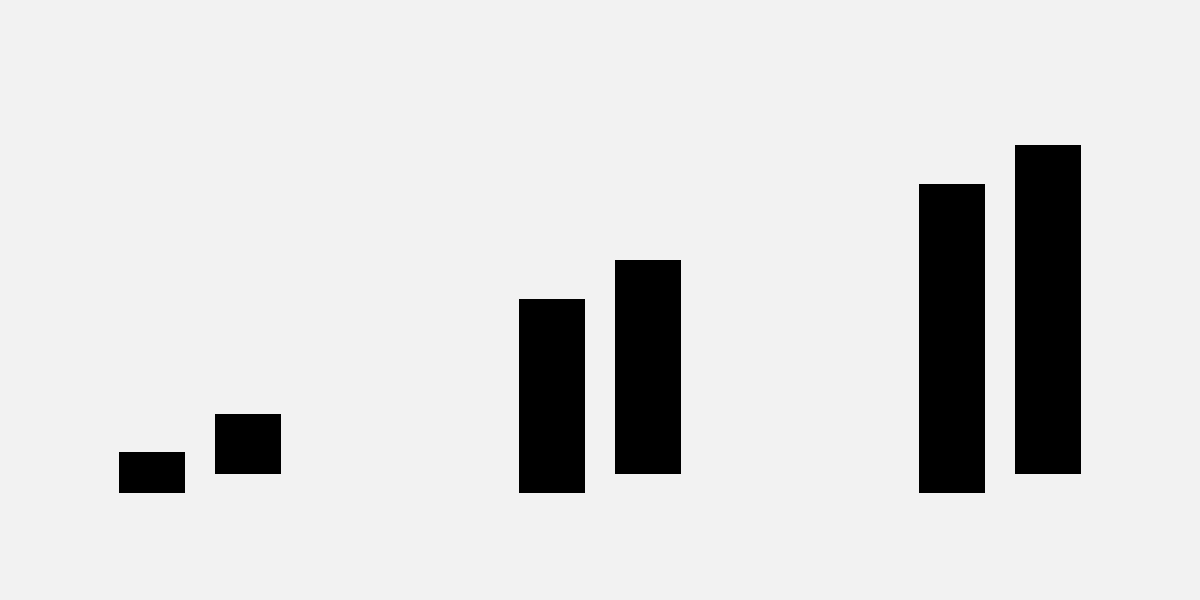
\includegraphics[width=1\linewidth,height=\textheight,keepaspectratio]{index_files/mediabag/quantitative_files/figure-pdf/fig-relative-1.pdf}

}

\caption{\label{fig-relative}A demonstration that perception of
differences is relative. The pairs of bars all differ by the same
absolute amount, but the difference is more easily perceived when
comparing the shorter bars. In the shorter bars, the absolute difference
between the bars is a larger difference relative to the length of the
bars.}

\end{figure}%

Figure~\ref{fig-relative-ref} shows that we can make it easier to judge
the differences by providing reference marks. Each pair of black bars is
the same and each pair of bars differs in length by the same small
amount. The difference between the bars in each pair is difficult to
perceive because the difference is small relative to the lengths of the
bars. The reference marks in the middle and right-hand pair of bars
provide shorter lengths to compare, so we are able to more easily
perceive the small differences. For example, for the pair of bars on the
right, we can compare the lengths of the short white gaps rather than
comparing the longer black bars.

\begin{figure}

\centering{

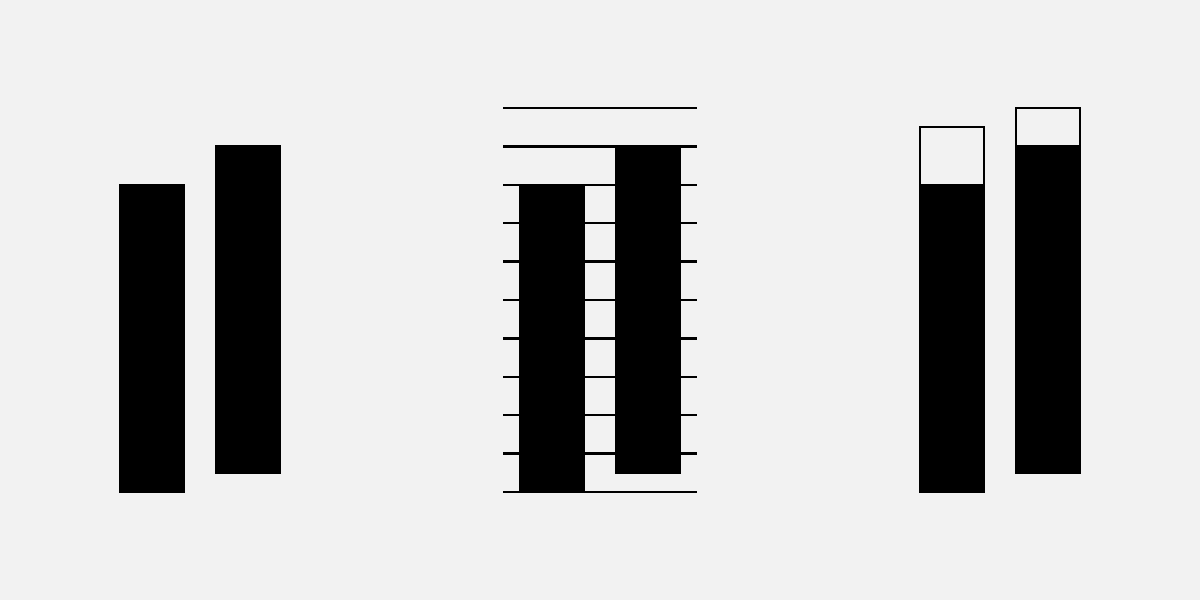
\includegraphics[width=1\linewidth,height=\textheight,keepaspectratio]{index_files/mediabag/quantitative_files/figure-pdf/fig-relative-ref-1.pdf}

}

\caption{\label{fig-relative-ref}A demonstration that reference marks
can make it easier to perceive small differences. Each pair of black
bars is the same and each pair differs by a small amount. In the middle
pair, grid lines make it easier to compare the distances from the ends
of the bars to the nearest grid line and, in the right-hand pair, a
border added to each bar, where the two borders are the same length,
makes it easier to compare the white gaps rather than the bars
themselves.}

\end{figure}%

Figure~\ref{fig-bar-district-grid} shows a bar plot of the number of
offenders in each police district (Figure~\ref{fig-bar-district}) with
some grid lines added. Although it is difficult to compare the bars for
Northland and Tasman because they are quite far apart and there are
distractors in between (Section~\ref{sec-distance-effect}), the addition
of the grid lines makes it easier to perform the comparison because we
are able to compare the distances from the ends of the bars to the
nearest grid line. Those distances are much shorter than the bars so it
is easier to perceive the small difference.

\begin{figure}

\centering{

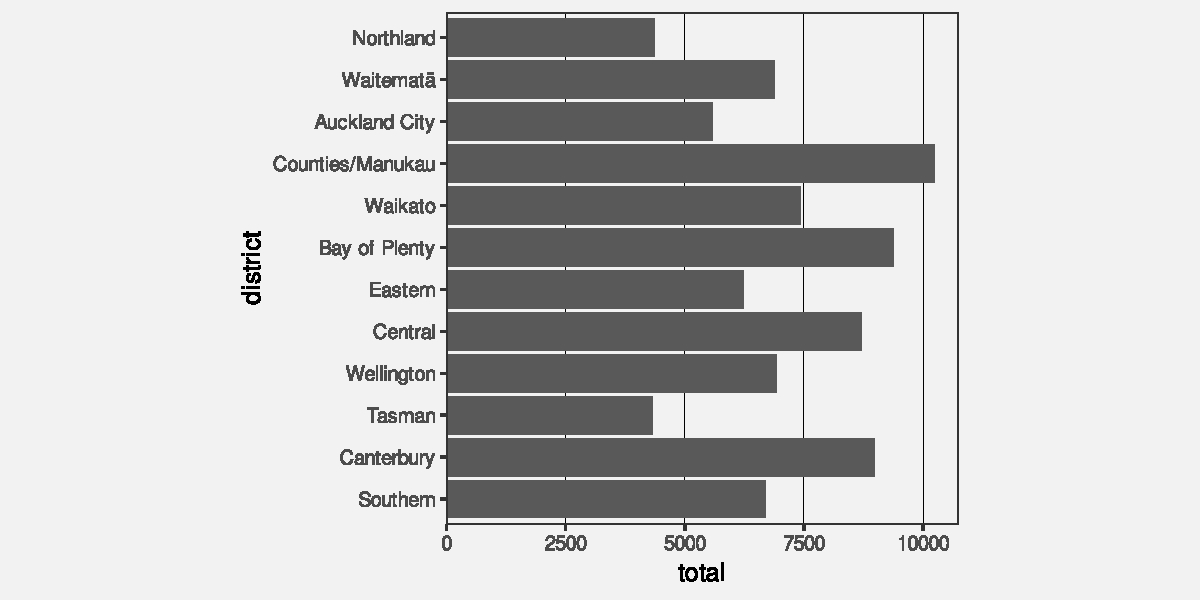
\includegraphics[width=1\linewidth,height=\textheight,keepaspectratio]{index_files/mediabag/quantitative_files/figure-pdf/fig-bar-district-grid-1.pdf}

}

\caption{\label{fig-bar-district-grid}A bar plot of the number of
offenders for different police districts, with the districts ordered
from North to South. This is very similar to
Figure~\ref{fig-bar-district}, just with some grid lines added.}

\end{figure}%

\begin{quote}
One reason why grid lines are effective is because they allow
comparisons of smaller lengths or distances, which means that it is
easier to perceive smaller changes.
\end{quote}

\section{Summary}\label{summary-4}

Bar plots are effective because they encode \textbf{quantitative} values
as \textbf{lengths}, which are accurate visual features.

However, comparisons between the bars in a bar plot can be difficult if
the bars are far apart, especially if there are distractors in between.

Furthermore, \textbf{stacked bars} are more difficult to compare because
they require comparing \textbf{unaligned} lengths.

Finally, it is easier to perceive differences between shorter bars than
between longer bars because the perception of differences is
\textbf{relative}.

\textbf{Grid lines} can help with comparisons because they make the
distances being compared smaller, so smaller differences are easier to
detect.

\begin{center}\rule{0.5\linewidth}{0.5pt}\end{center}

\theendnotes

\bookmarksetup{startatroot}

\chapter{Colour}\label{colour}

Figure~\ref{fig-pie-hue} shows a pie chart of the number of offenders
for different levels of crime seriousness (between 2011 and 2021). In
this data visualisation, the crime level, which is a
\textbf{qualitative} variable, is encoded as \textbf{colour}, which is
appropriate for representing qualitative values (see
Section~\ref{sec-qual-features}). It is easy to identify different crime
levels because it is easy to perceive differences between the colours of
the wedges in the pie chart.

\begin{figure}

\centering{

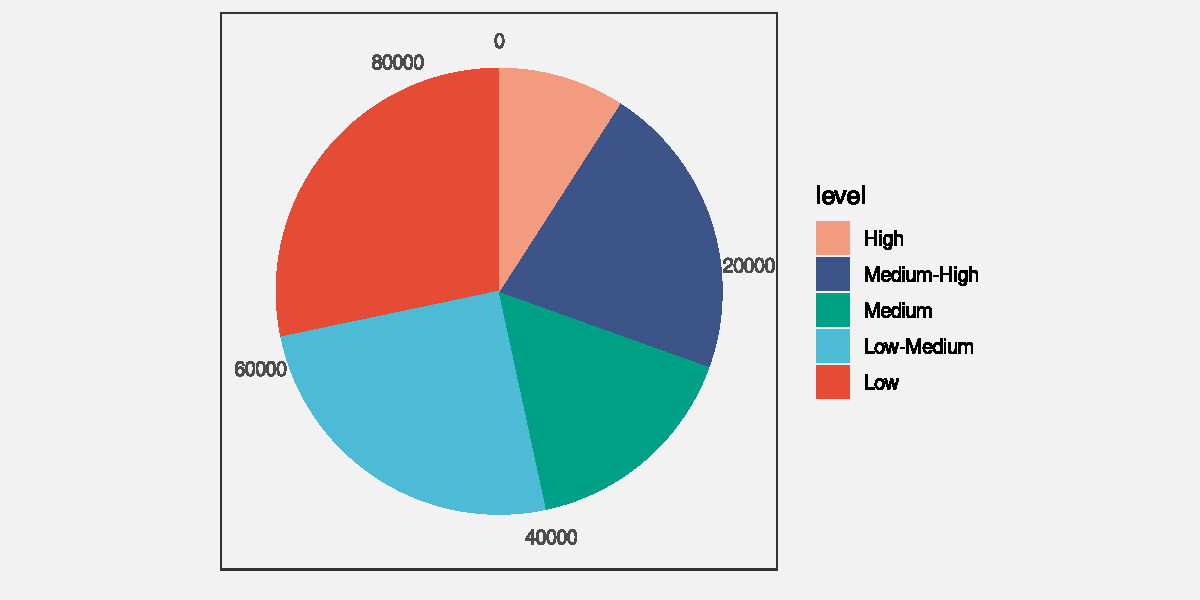
\includegraphics[width=1\linewidth,height=\textheight,keepaspectratio]{index_files/mediabag/qualitative_files/figure-pdf/fig-pie-hue-1.pdf}

}

\caption{\label{fig-pie-hue}A data visualisation of the number of
offenders for different levels of crime seriousness.}

\end{figure}%

Figure~\ref{fig-pie-ordinal} shows another pie chart of the same data,
again encoding the \textbf{qualitative} level as \textbf{colour}. It is
again easy to differentiate between different crime levels because we
can easily perceive differences between the colours of the wedges.
However, Figure~\ref{fig-pie-ordinal} is \emph{more} effective than
Figure~\ref{fig-pie-hue} because we can \emph{also} perceive an ordering
of the wedges from more serious crimes, which are darker wedges, to less
serious crimes, which are lighter wedges.

\begin{figure}

\centering{

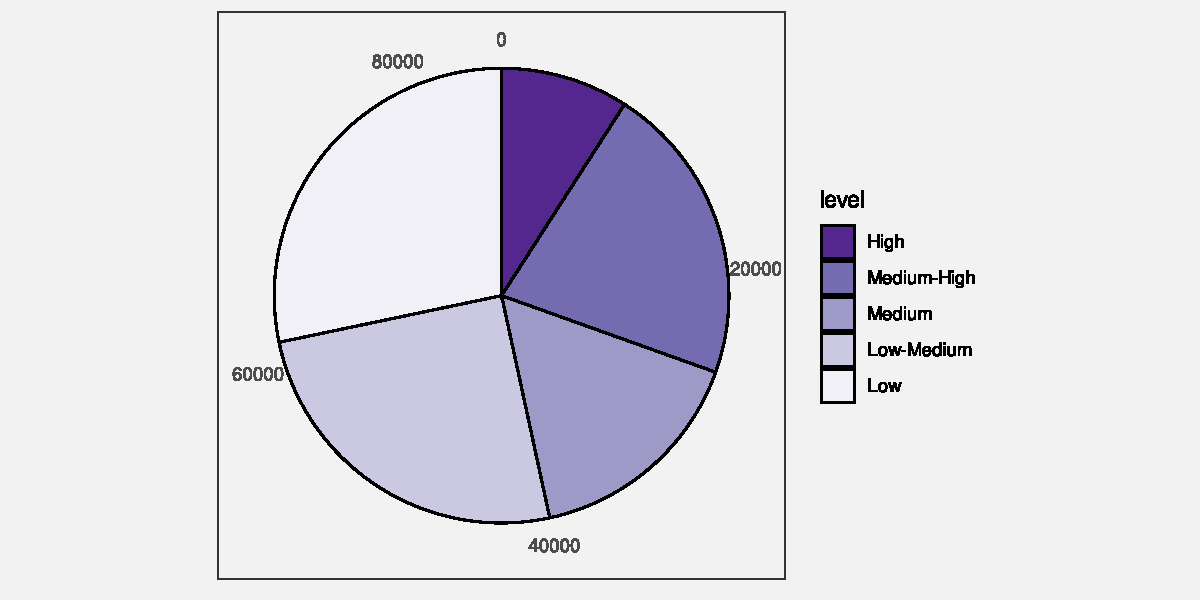
\includegraphics[width=1\linewidth,height=\textheight,keepaspectratio]{index_files/mediabag/qualitative_files/figure-pdf/fig-pie-ordinal-1.pdf}

}

\caption{\label{fig-pie-ordinal}A data visualisation of the number of
offenders for different levels of crime seriousness.}

\end{figure}%

The fact that there can be two data visualisations,
Figure~\ref{fig-pie-hue} and Figure~\ref{fig-pie-ordinal}, with the same
mapping, the \textbf{qualitative} level of crime is encoded as the
visual feature \textbf{colour}, but the two data visualisations have
different effectiveness suggests that there is still more to learn about
how different visual features work.

This section covers some more details about how the \textbf{colour}
visual feature works.

\section{Hue, chroma, and luminance}\label{sec-colour}

We have so far taken a very simplistic approach to \textbf{colour},
treating it as if it is a single \textbf{qualitative} visual feature
(Section~\ref{sec-qual-features}). However, the perception of colour can
be divided into three separate visual features: \textbf{hue},
\textbf{chroma}, and \textbf{luminance}
(Figure~\ref{fig-hcl}).\footnote{The three-dimensional experience of
  colour arises from the fact that there are three different sorts of
  cones in the retina (see Section~\ref{sec-eye}), each sensitive to a
  different range of light wavelengths: The L cones respond to long
  wavelengths (reds); the M cones respond to medium wavelengths
  (greens); and the S cones respond to short wavelengths (blues). The
  neural connections that combine the messages from the retina are also
  divided into three pathways: light-dark, which represents the sum of
  L, M, and S cones; red-green, which represents the difference between
  L and M cones; and blue-yellow, which represents the difference
  between S cones and the sum of L and M cones. For more information,
  see Ware (2021).} Hue describes what we normally refer to as the
colour name: reds, oranges, yellows, greens, blues, and purples. Chroma
describes the colourfulness, from bright to dull, and luminance
describes the lightness, from dark to light. Our visual system is
capable to perceiving changes in hue and changes in chroma and changes
in luminance.

We have described colour as a \textbf{qualitative} visual feature so
far, but that really strictly only applies to \textbf{hue}. For example,
Figure~\ref{fig-stacked-bar} used different hues to represent different
ethnic groups. Hue is excellent for the perception of differences.

\begin{figure}

\centering{

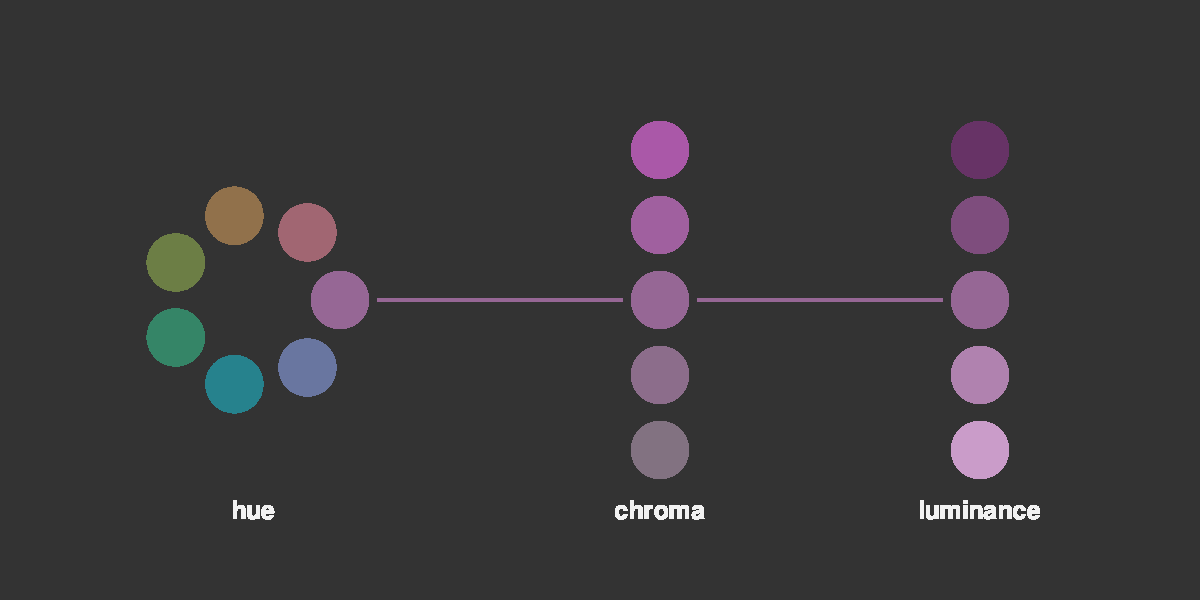
\includegraphics[width=1\linewidth,height=\textheight,keepaspectratio]{index_files/mediabag/qualitative_files/figure-pdf/fig-hcl-1.pdf}

}

\caption{\label{fig-hcl}The perception of colour can be divided into
three components: differences in \textbf{hue}, the colours of the
rainbow; differences in \textbf{chroma}, from bright and colourful to
dull and grey; and differences in \textbf{luminance}, from light to
dark.}

\end{figure}%

\section{Ordinal visual features}\label{sec-ordinal}

\textbf{Chroma} and \textbf{luminance} are both \textbf{nominal} visual
features in that they can be used to visualise different groups, but
they are also \textbf{ordinal} visual features because we can perceive
an ordering from a set of colours that differ in terms of either chroma
or luminance or both. A set of colours that transitions from darker to
lighter and/or brighter to duller conveys an ordering from larger to
smaller.\footnote{``Mapping Color to Meaning in Colormap Data
  Visualizations'' Schloss et al (2018) Evidence for dark-is-more bias

  ``More of what? Dissociating effects of conceptual and numeric
  mappings on interpreting colormap data visualizations'' Soto et al
  (2023) Evidence for dark-is-more bias}

This helps to explain why Figure~\ref{fig-pie-ordinal} is more effective
than Figure~\ref{fig-pie-hue}. In Figure~\ref{fig-pie-ordinal}, the
colours differ mostly in terms of luminance and chroma so we are able to
perceive changes from larger values to smaller values because the
colours transition from darker to lighter.

In this sense, \textbf{chroma} and \textbf{luminance} are able to convey
more information than \textbf{hue} because they can represent
\textbf{nominal} differences \emph{and} \textbf{ordinal} differences,
whereas hue can only represent nominal differences.

On the other hand, Figure~\ref{fig-lum-cap} shows that chroma and
luminance are even more limited than hue in terms of \textbf{capacity}.
We can only use chroma and/or luminance to represent \textbf{nominal}
data when there are very few different groups to represent.

\begin{figure}

\centering{

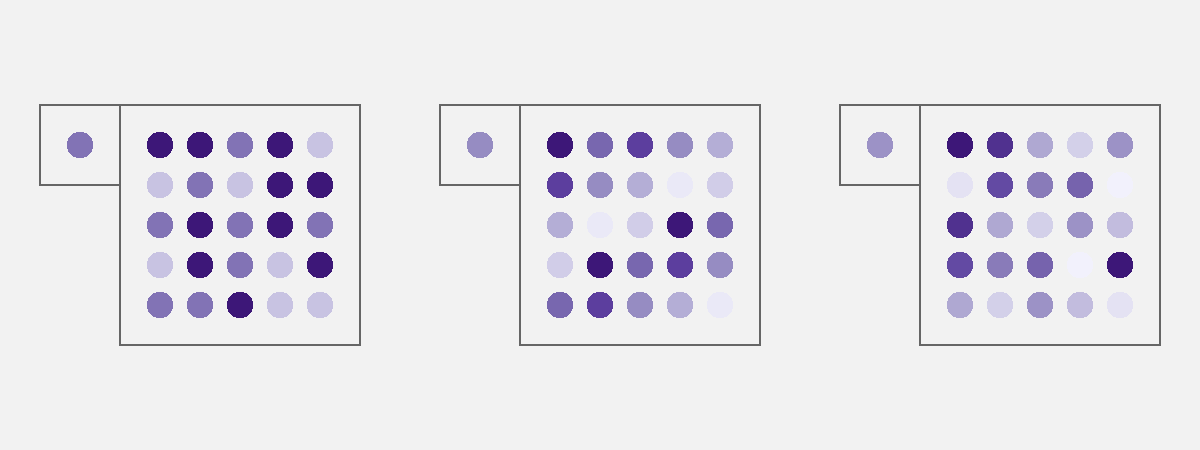
\includegraphics[width=1\linewidth,height=\textheight,keepaspectratio]{index_files/mediabag/qualitative_files/figure-pdf/fig-lum-cap-1.pdf}

}

\caption{\label{fig-lum-cap}Mapping qualitative values to luminance and
chroma works well for representing nominal data values, but only for a
very small number of values. The three values on the left are easily
distringuishable, but it becomes difficult to clearly distinguish
between adjacent colours in the middle and almost impossible for the
colours on the right. This figure can be compared with
Figure~\ref{fig-colour-cap}, which demonstrates the capacity of hue for
representing nominal data values.}

\end{figure}%

\section{Perception is relative}\label{sec-colour-relative}

We saw in Section~\ref{sec-perception-relative} that perception of
\textbf{lengths} is relative. For example, smaller differences in length
are easier to see when the lengths themselves are short (see
Figure~\ref{fig-relative}).

There is a similar rule for the perception of \textbf{colours}. Our
perception of luminance and chroma is affected by neighbouring
colours.\footnote{This relative perception of colours is useful for
  being able to adapt to a wide range of lighting conditions. See Ware
  (2021) for a more detailed discussion.} This effect is demonstrated in
Figure~\ref{fig-contrast-effect}: the same colour when surrounded by a
darker background appears lighter than it does when surrounded by a
lighter background.

\begin{figure}

\centering{

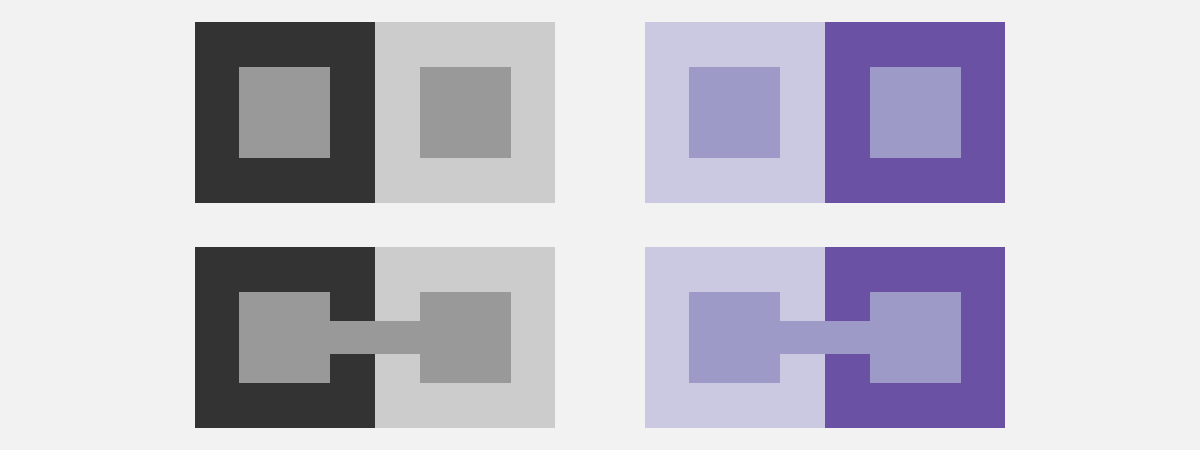
\includegraphics[width=1\linewidth,height=\textheight,keepaspectratio]{index_files/mediabag/qualitative_files/figure-pdf/fig-contrast-effect-1.pdf}

}

\caption{\label{fig-contrast-effect}The perception of colours is
relative. In the top row, the inner rectangles are exactly the same
shade of grey on the left and exactly the same shade of purple on the
right. The perception of the inner rectangles is affected by the
surrounding colour, so the same shade appears darker against a light
background and darker against a light background. The bottom row draws a
line connecting the two inner rectangles to show that they really are
the same shade.}

\end{figure}%

This effect also applies to the perception of hue.
Figure~\ref{fig-pie-contrast} shows a pie chart of the number of
offenders in each police district, with police district mapped to the
\textbf{colour} of the wedges. There are two issues with the perception
of the wedge colours: each wedge is affected by its neighbour so that,
for example, some of the blue wedges look more green at the boundary
with their more blue neighbour and more blue at the boundary with their
more green neighbour; furthermore, the colours in the legend are
perceived differently from the corresponding colours in the wedges
because the legend colours are surrounded by a light grey, rather than
sharing a boundary with a neighbouring colour.

\begin{figure}

\centering{

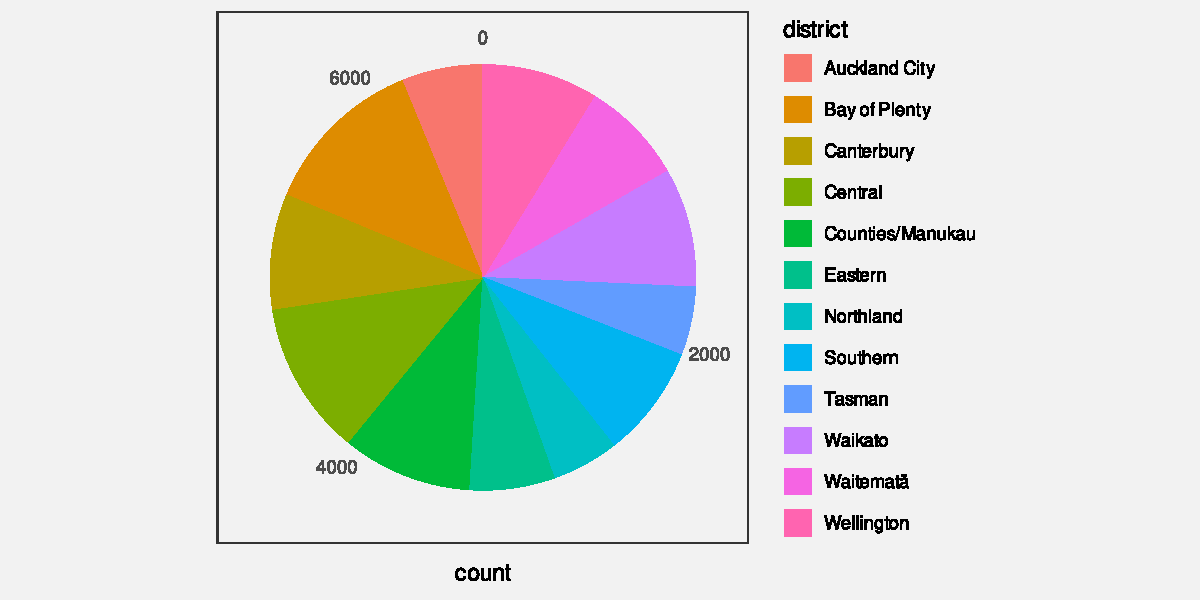
\includegraphics[width=1\linewidth,height=\textheight,keepaspectratio]{index_files/mediabag/qualitative_files/figure-pdf/fig-pie-contrast-1.pdf}

}

\caption{\label{fig-pie-contrast}This pie chart demonstrates that the
perception of hues is relative. The colours within each wedge appear to
have a subtle gradient within the wedge because the perception of the
wedge colour is affected differently by the neighbouring wedge colours.}

\end{figure}%

The pie chart in Figure~\ref{fig-pie-contrast} is \emph{not} an
effective data visualisation because it encodes qualitative data values
with many different groups as colour hue. This exceeds the
\textbf{capacity} of the \textbf{hue} visual feature; it is difficult to
clearly distinguish between all of the different hues (see
Section~\ref{sec-capacity}).

Although it does not make the use of hue any more appropriate, for the
purposes of demonstration, we can solve the colour perception problems
in Figure~\ref{fig-pie-contrast} by adding a white border to all of the
wedges (see Figure~\ref{fig-pie-contrast-solved}). Now all of the wedges
and all of the squares in the legend are perceived relative to a
surrounding white border.

\begin{figure}

\centering{

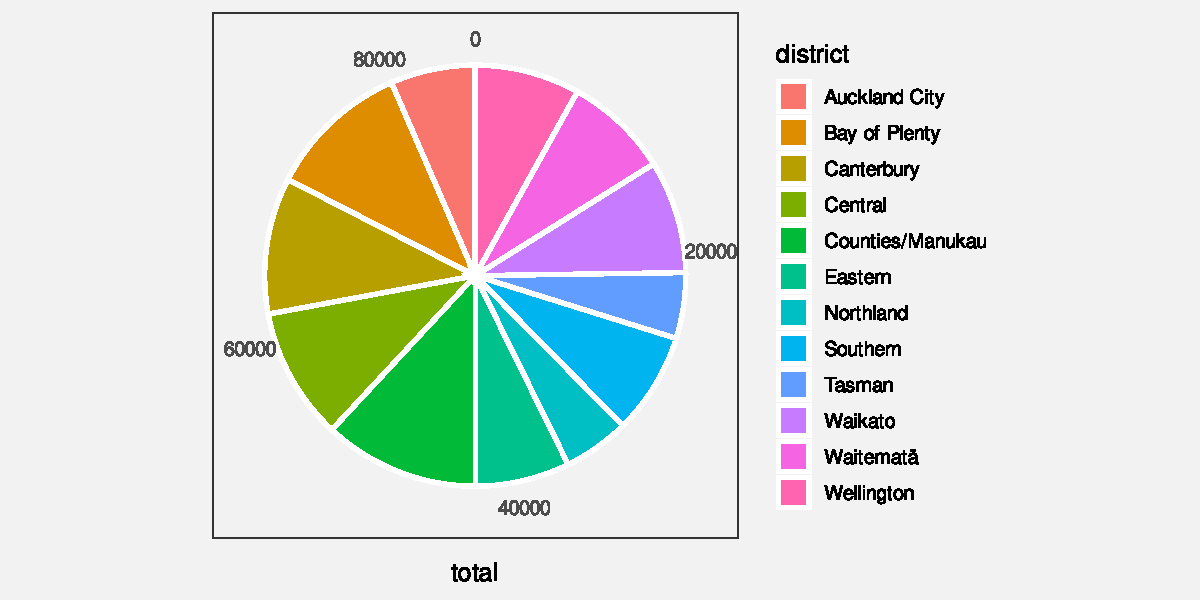
\includegraphics[width=1\linewidth,height=\textheight,keepaspectratio]{index_files/mediabag/qualitative_files/figure-pdf/fig-pie-contrast-solved-1.pdf}

}

\caption{\label{fig-pie-contrast-solved}The hues in this pie chart are
perceived more accurately than those in Figure~\ref{fig-pie-contrast}
because each wedge is surrounded by a white border.}

\end{figure}%

\section{Colour vision deficiency}\label{sec-CVD}

Roughly 10\% of the population, primarily men, suffer from a form of
colour vision deficiency.\footnote{Provide a cite for those percentages}
In the most common case, the viewer will have difficulty distinguishing
between red and green hues. Figure~\ref{fig-pie-hue-cvd} simulates how
the colours in Figure~\ref{fig-pie-hue} would appear to a person with
severe deuteranopia (red-green colour blindness).

\begin{figure}

\centering{

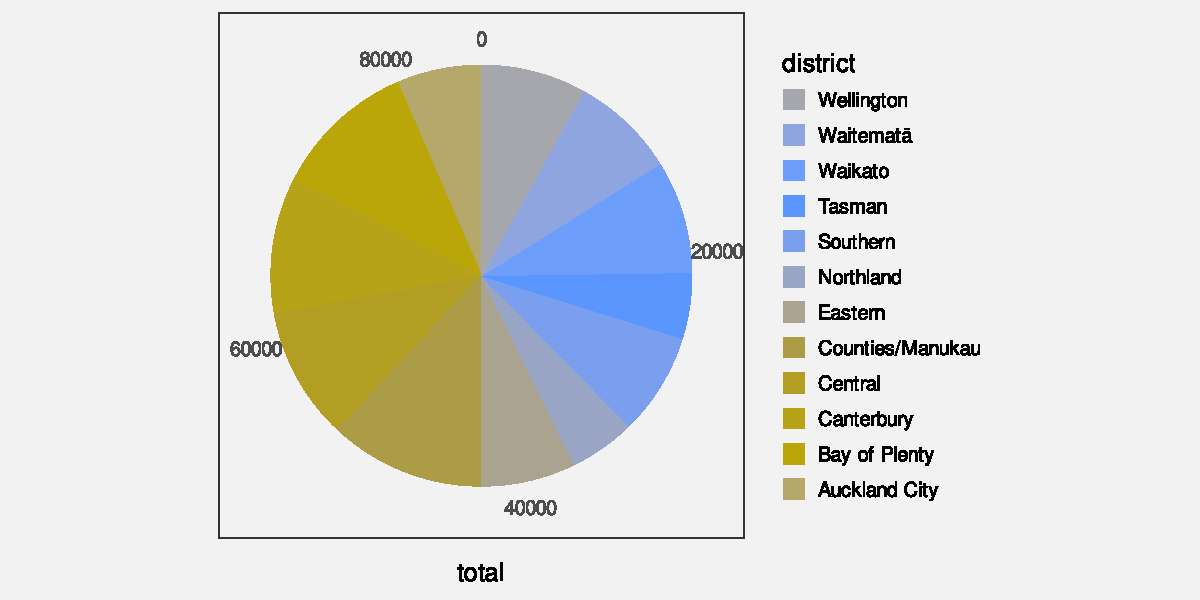
\includegraphics[width=1\linewidth,height=\textheight,keepaspectratio]{index_files/mediabag/qualitative_files/figure-pdf/fig-pie-hue-cvd-1.pdf}

}

\caption{\label{fig-pie-hue-cvd}A data visualisation of the number of
offenders for different levels of crime seriousness.}

\end{figure}%

In order to avoid confusion for viewers with CVD, it may be necessary to
vary luminance and/or chroma in addition to or instead of hue. For
example, Figure~\ref{fig-pie-ordinal-cvd} shows how the shades of purple
in Figure~\ref{fig-pie-ordinal} would appear to a viewer with severe
deuteranopia. The difference in hue is of no importance in this case.

\begin{figure}

\centering{

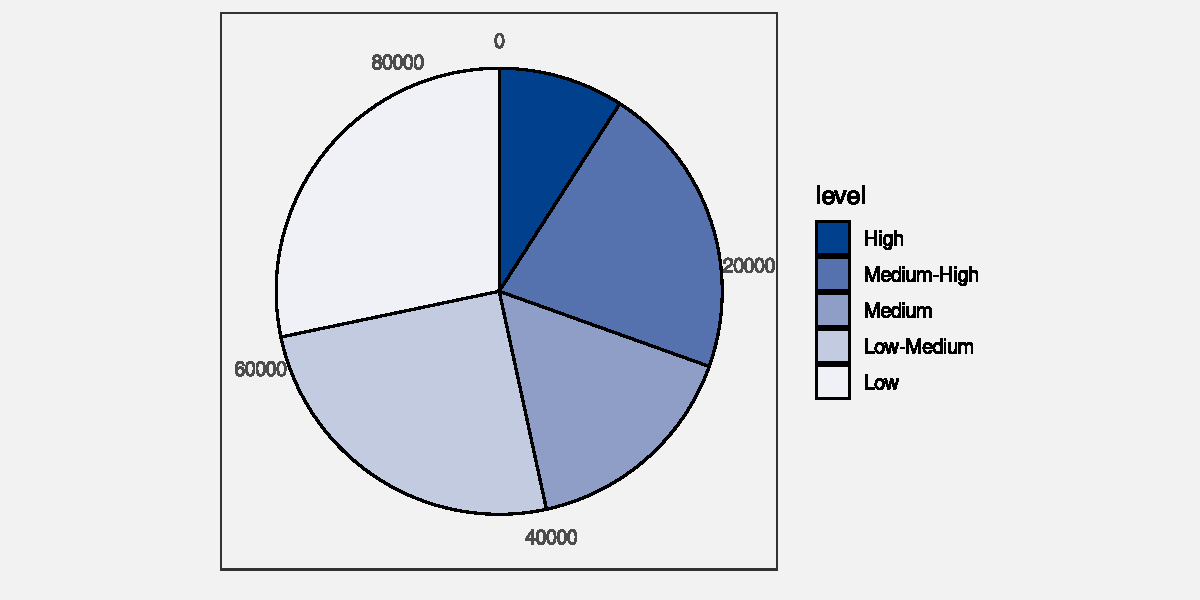
\includegraphics[width=1\linewidth,height=\textheight,keepaspectratio]{index_files/mediabag/qualitative_files/figure-pdf/fig-pie-ordinal-cvd-1.pdf}

}

\caption{\label{fig-pie-ordinal-cvd}A data visualisation of the number
of offenders for different levels of crime seriousness.}

\end{figure}%

\section{Size matters}\label{size-matters}

The perception of colours is also affected by the size of the coloured
region. In particular, small regions of colour may blend together with
neighbouring colours. \footnote{``In Color Perception, Size Matters''
  Stone (2012) ``In designing colors for digital visualization systems.
  one of the most critical factors is the interaction between size and
  color appearance.'' Talks about ``spreading'', which means a sort of
  blending or averaging of colours over small areas \emph{by the visual
  system}.} For example, on the left of Figure~\ref{fig-colour-size},
the yellow and blue stripes are the same colours both in the top set if
wide bars and in the bottom set of narrow bars. The right side of
Figure~\ref{fig-colour-size} shows that the same colours may appear
different when they are used as fill colours for larger regions, like
bars, compared to when they are used for thin lines.

\begin{figure}

\centering{

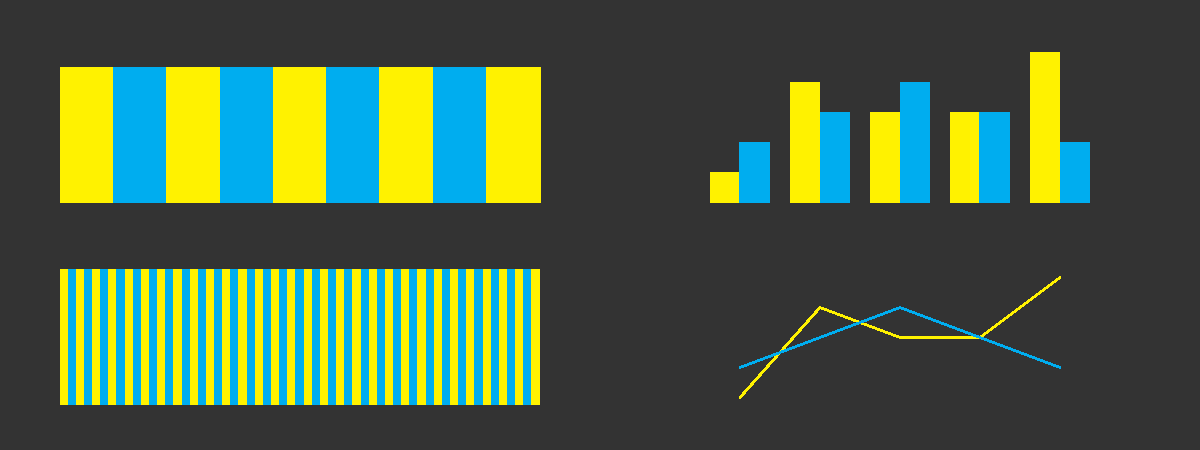
\includegraphics[width=1\linewidth,height=\textheight,keepaspectratio]{index_files/mediabag/qualitative_files/figure-pdf/fig-colour-size-1.pdf}

}

\caption{\label{fig-colour-size}The perception of colours varies based
on the size of the coloured regions.}

\end{figure}%

\section{Colour palettes}\label{colour-palettes}

When we encode nominal or ordinal data values as colours, we have to
choose a set of colours, or a \textbf{colour palette}. For example, in
Figure~\ref{fig-pie-hue} we have to choose a different colour to
represent each level of crime.

This choice is difficult because there are many different colours to
choose from and often there is no obvious mapping from a data value to a
particular colour. For example, what specific hue, chroma, and luminance
should we choose to represent a \texttt{high} crime level?

There are also competing criteria involved in selecting colours. For
example, although the primary goal is to represent different categories
with colours that are as different from each other as possible, we also
have to take into account that some viewers may have difficulty
perceiving differences between particular colours
(Section~\ref{sec-CVD}).

Fortunately, researchers have produced a number of predefined colour
palettes that we can make use of.\footnote{cite R Journal article with
  Achim} For example, the colours used in Figure~\ref{fig-pie-hue} are
based on palettes used in journals published by the Nature Publishing
Group.\footnote{cite ggsci, colour brewer (and others?)} There are also
many helpful tools online.\footnote{https://color.adobe.com/}

If the data symbols are arranged in a regular pattern, like in a bar
plot, then comparisons between neighbours are most important, so we can
order the colours to maximise neighbour differences rather than
maximising all pairwise differences.\footnote{``Reflections on the Uses
  and Available Choices of Categorical Colorschemes'' Bartolomeo et al
  (2025)} Figure~\ref{fig-pie-order} demonstrates this idea with a bar
plot of the crime rate in different districts for both 2011 and 2021.
This bar plot uses the same set of hues as
Figure~\ref{fig-pie-contrast-solved}, just in a different order so that
adjacent bars have very different colours.

\begin{figure}

\centering{

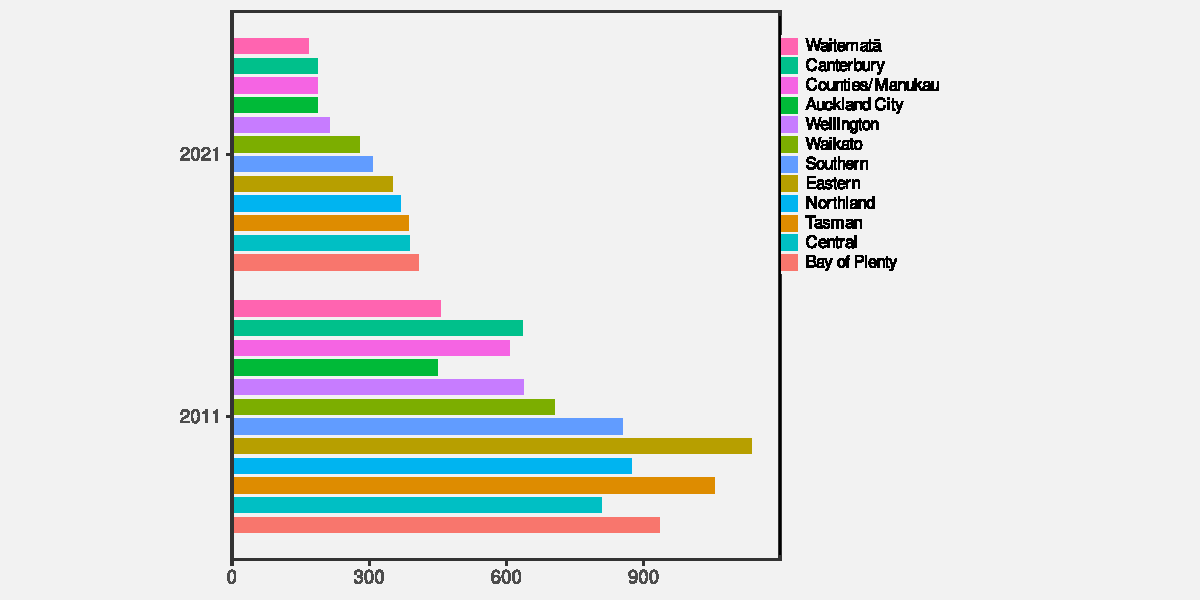
\includegraphics[width=1\linewidth,height=\textheight,keepaspectratio]{index_files/mediabag/qualitative_files/figure-pdf/fig-pie-order-1.pdf}

}

\caption{\label{fig-pie-order}The hues in this pie chart are ordered so
that adjacent hues are distant from each other.}

\end{figure}%

A similar idea is to just reuse a smaller set of hues, which means
larger differences between adjacent colours, but repeat the set. The
regular arrangement of the data symbols means that we can still
differentiate between repeated colours because of the bar positions
(Figure~\ref{fig-pie-repeat}). For example, we can differentiate the
pink for the Wellington district from the pink for the Eastern district
because Wellington is at the end and Eastern is in the middle.

\begin{figure}

\centering{

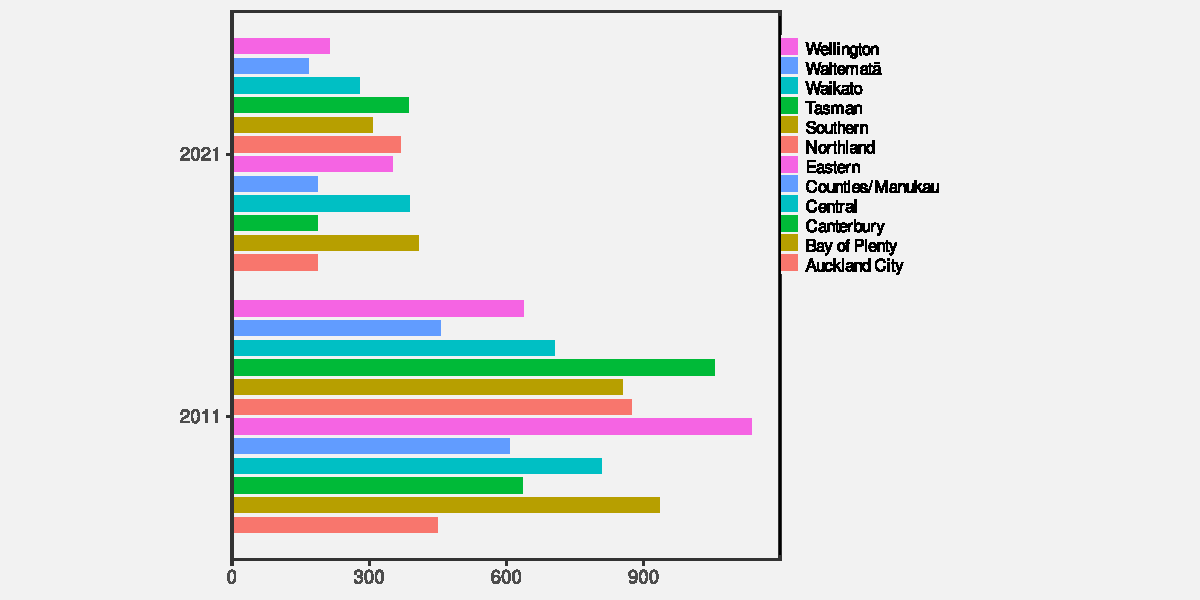
\includegraphics[width=1\linewidth,height=\textheight,keepaspectratio]{index_files/mediabag/qualitative_files/figure-pdf/fig-pie-repeat-1.pdf}

}

\caption{\label{fig-pie-repeat}The hues in this pie chart are repeated
so that adjacent hues are more distant from each other.}

\end{figure}%

\section{Case study: Divergent colour
palettes}\label{case-study-divergent-colour-palettes}

The Rugby World Cup is a competition that is held every four years, with
the first event taking place in 1987. We have data on the total number
of points that were scored and conceded in World Cup matches for Tier
One nations (the top 10 rugby-playing nations) at each World Cup.
Table~\ref{tbl-rwc-all-year} shows a sample of these data.\footnote{Attribution
  to kaggle data set.}

\begin{longtable}[]{@{}lrrrr@{}}

\caption{\label{tbl-rwc-all-year}A table of the total number of points
scored and conceded by Tier One nations in Rugby World Cup matches at
each World Cup. Each row represents thetotal points scored by one team
in one World Cup. There are 100 rows in total, with just the first 6
rows shown here.}

\tabularnewline

\toprule\noalign{}
team & year & scored & conceded & diff \\
\midrule\noalign{}
\endhead
\bottomrule\noalign{}
\endlastfoot
Italy & 1987 & 22 & 95 & -73 \\
Italy & 1991 & 27 & 67 & -40 \\
Italy & 1995 & 51 & 52 & -1 \\
Italy & 1999 & 10 & 168 & -158 \\
Italy & 2003 & 22 & 97 & -75 \\
Italy & 2007 & 30 & 94 & -64 \\

\end{longtable}

Figure~\ref{fig-neg-tile} shows a heatmap of the points differential
(points scored for minus points scored against) for Tier One nations at
each Rugby World Cup. The data symbols are rectangles, or ``tiles''. The
teams are encoded as the vertical \textbf{positions} of the tiles and
the years are encoded as the horizontal \textbf{positions} of the tiles.
These are both effective mappings and we can easily \textbf{decode} to
teams or years. The points differentials are encoded as the
\textbf{colour} of the tiles, but in a slightly complicated way.
Positive data values map to a shade of purple, while negative values map
to a shade of brown. In both cases, we have a constant \textbf{hue},
with increasing \textbf{chroma} and decreasing \textbf{luminance} as the
data values get further away from zero.

The use of two \textbf{hues} creates two different groups (positive and
negative values), while the changes in \textbf{chroma} and
\textbf{luminance} convey changes in absolute magnitude (if only for
ordinal comparisons).

\begin{figure}

\centering{

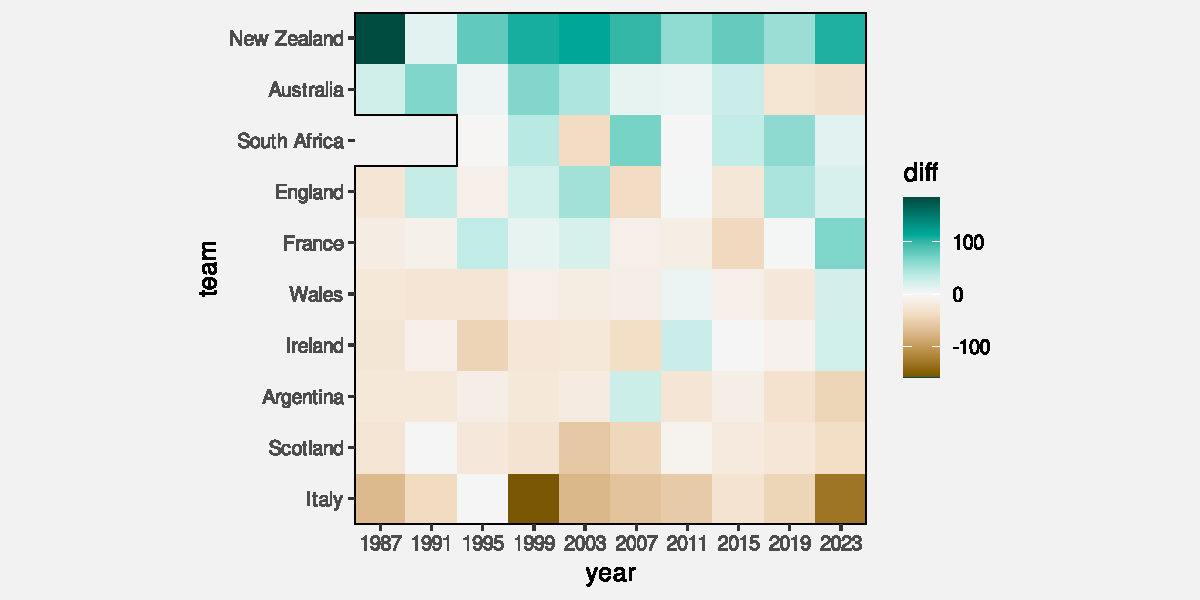
\includegraphics[width=1\linewidth,height=\textheight,keepaspectratio]{index_files/mediabag/qualitative_files/figure-pdf/fig-neg-tile-1.pdf}

}

\caption[\label{fig-neg-tile}A heatmap of the total points differentials
for Tier One nations at individual Rugby World Cups. South Africa was
excluded from the 1987 and 1991 tournament due to its apartheid
policies.]{\label{fig-neg-tile}A heatmap of the total points differentials
for Tier One nations at individual Rugby World Cups. South Africa was
excluded from the 1987 and 1991 tournament due to its apartheid
policies.\footnotemark{}}

\end{figure}%
\footnotetext{The \{gggrid\} package (Murrell 2022) was used to
  take the ``bite'' out of the panel border in Figure~\ref{fig-neg-tile}
  where South Africa was excluded.}

\begin{quote}
A diverging colour palette is effective because it creates two distinct
visual features: a nominal hue to differentiate between two groups and
changes in chroma and/or luminance to encode ordinal values within each
group.
\end{quote}

\section{Summary}\label{summary-5}

\textbf{Colour} is really three visual features: \textbf{hue},
\textbf{chroma}, and \textbf{luminance}.

\textbf{Hue} is excellent for representing \textbf{nominal} data values.

\textbf{Chroma} and \textbf{luminance} can be used to represent
\textbf{ordinal} data values, but they have a very limited capacity.

We should lean on the work done by experts when it comes to choosing
colour palettes.

\begin{center}\rule{0.5\linewidth}{0.5pt}\end{center}

\theendnotes

\bookmarksetup{startatroot}

\chapter{Congruent Mappings}\label{sec-congruence}

The purpose of this section is to show that we need to consider more
than just the accuracy or capacity of our mappings from data values to
basic visual features in order to understand the effectiveness of a data
visualisation.\footnote{Tversky, Morrison, and Betrancourt (2002)
  discusses congruence at least in the sense of matching the spatial
  properties of data values to the spatial arrangement of visual
  features. The concept is also discussed in Bertini, Correll, and
  Franconeri (2020).}

\section{Implicit mappings}\label{sec-implicit}

Sort of like pre-attentive analogue of learned decodings.

Do a simple example - maybe just the fact that a bar twice the length of
another bar is perceived as ``twice'' !? These implicit mappings are the
basis of whether visual features are quant or qual!?

\begin{figure}

\centering{

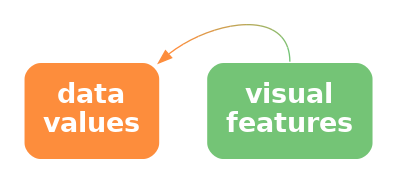
\includegraphics[scale=0.5]{Diagrams/implicit-decode.png}

}

\caption{\label{fig-implicit-decode}Some visual features have implicit
encodings, which means that we can decode values from the visual
features without having explicitly encoded values as visual features.}

\end{figure}%

When an implicit encoding exists, we can produce a more effective
mapping by building upon the implicit decoding. We can explicitly encode
data values as visual features in such a way that the decoding is
\textbf{congruent} with the implicit decoding, in the sense that the
implicit decoding leads back to the original data values that we
explicitly encoded (Figure~\ref{fig-congruent-decode}).

\begin{figure}

\centering{

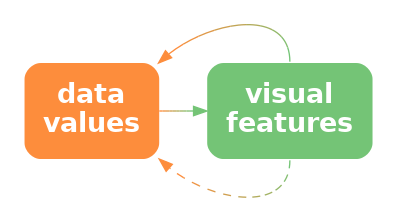
\includegraphics[scale=0.5]{Diagrams/congruent-decode.png}

}

\caption{\label{fig-congruent-decode}If we explicitly map data values to
visual features in a way that is consistent with an implicit mapping, we
can more effectively decode data values from visual features.}

\end{figure}%

\section{Part-to-whole}\label{sec-part-to-whole}

Figure~\ref{fig-prop} shows a pie chart of the proportions of total
youth offenders between 2011 and 2021 in different ethnic groups and a
bar plot of the same data. We learned in Section~\ref{sec-accuracy} that
encoding \textbf{quantitative} proportions as \textbf{lengths}, like in
the bar plot, is more accurate than encoding the proportions as
\textbf{angles} or \textbf{areas}, like in the pie chart.

However, the superior represenation of the fact that Māori offenders
make up approximately 50\% of the total is the pie chart rather than the
bar plot.

Although it is easy to determine from the length of the bar and the
scale on the x-axis in the bar plot that the bar for Māori is just below
0.5, it is even easier, without any guides at all, to see that the light
blue wedge in the pie chart is just under half a circle. It is also easy
to see that the red wedge is close to a third of a circle.\footnote{Simkin
  and Hastie (1987) found empirical evidence that people judge
  proportions better on pie charts than bar charts. So did Eells (1926).}

\begin{figure}

\begin{minipage}{0.50\linewidth}

\centering{

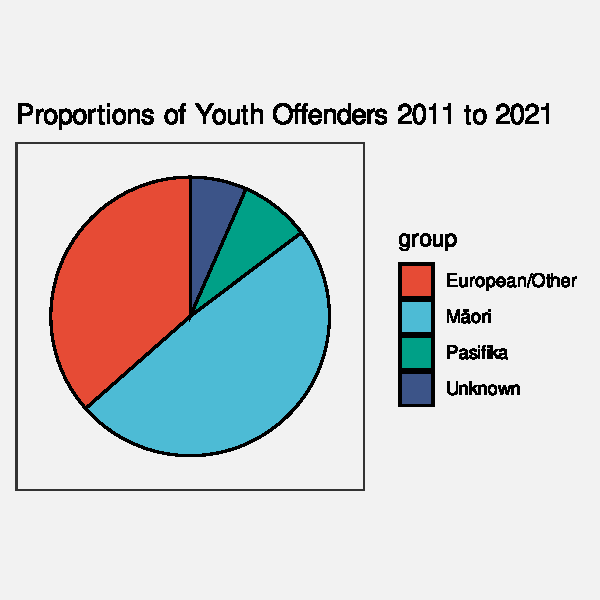
\includegraphics[width=1\linewidth,height=\textheight,keepaspectratio]{index_files/mediabag/congruence_files/figure-pdf/fig-prop-1.pdf}

}

\subcaption{\label{fig-prop-1}A pie chart.}

\end{minipage}%
%
\begin{minipage}{0.50\linewidth}

\centering{

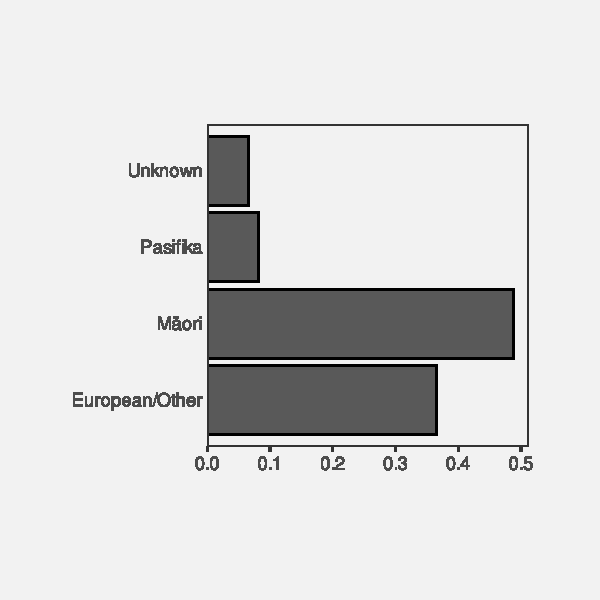
\includegraphics[width=1\linewidth,height=\textheight,keepaspectratio]{index_files/mediabag/congruence_files/figure-pdf/fig-prop-2.pdf}

}

\subcaption{\label{fig-prop-2}A bar plot.}

\end{minipage}%

\caption{\label{fig-prop}Data visualisations of the proportion of
offenders from different ethnic groups.}

\end{figure}%

The reason why the pie chart in Figure~\ref{fig-prop} is more effective
than a bar plot for conveying simple proportions like a quarter or a
third or a half is because the wedges in a pie chart have an implicit
decoding to fractions of a whole. A semi-circle has a strong visual
association with \emph{half} of a circle and thirds and quarters are
similarly evocative.

\begin{quote}
One reason why a pie chart can be effective is because segments of a pie
vividly convey simple fractions of a whole.
\end{quote}

Figure~\ref{fig-bar-part} shows that if we place a bar representing a
proportion bar within a reference rectangle that corresponds to a
proportion of 1, then we can also create a part-to-whole congruence with
bars, though the effect is not as strong as it is for pie wedges.

\begin{figure}

\centering{

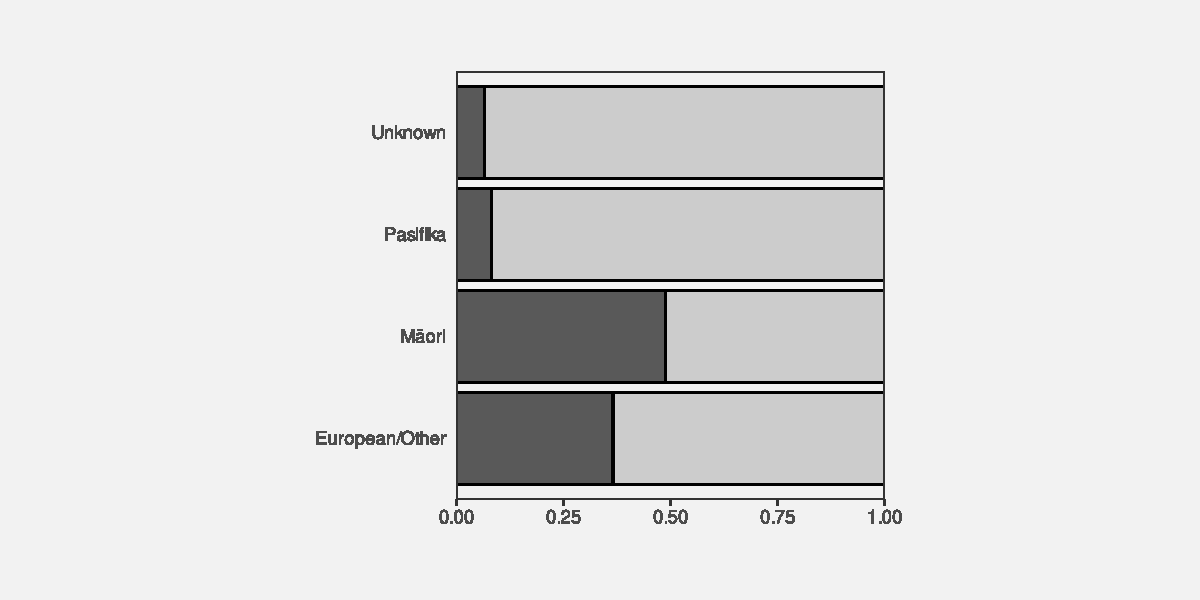
\includegraphics[width=1\linewidth,height=\textheight,keepaspectratio]{index_files/mediabag/congruence_files/figure-pdf/fig-bar-part-1.pdf}

}

\caption{\label{fig-bar-part}A bar plot of the proportion of offenders
from different ethnic groups with reference rectangles to enhance the
part-to-whole relationship.}

\end{figure}%

\section{More is more}\label{sec-more-is-more}

We saw in Section~\ref{sec-quant-features} that visual features like
\textbf{length} and \textbf{area} are appropriate for conveying
quantitative values. For example, in Figure~\ref{fig-more-is-more}, the
lengths of the bars are appropriate for conveying the total number of
offenders in different ethnic groups.

Part of the reason why \textbf{length} and \textbf{area} work so well is
because a \textbf{longer} bar naturally conveys the idea of
\textbf{more}.\footnote{Wilke's Principle of Proportional Ink. ChatGPT
  attributed this to Wilkinson (GoG), but I cannot find the reference
  anywhere. Wilke attributes this to Bergstrom, C. T., and J. West.
  2016. ``The Principle of Proportional Ink.''
  http://callingbullshit.org/tools/tools\_proportional\_ink.html. A
  corollary is that bars should start at zero.

  Kosslyn (2006) ``Graph Design for the Eye and Mind''
  ./Resources/Graph-Design-for-the-Eye-and-Mind/appendix-3.pdf Principle
  of Compatibility says ``A message is easiest to understand if its form
  is compatible with its meaning'', plus explicitly ``more is more''} By
contrast, the \textbf{position} of data points in a dot plot of the same
data, as shown in Figure~\ref{fig-more-is-more}, do not inherently
convey the same sense of \emph{more}. In a bar plot, the data symbols
that correspond to larger data values are actually larger data symbols;
the presentation of larger data values is more abstract in a dot plot.

\begin{figure}

\begin{minipage}{0.50\linewidth}

\centering{

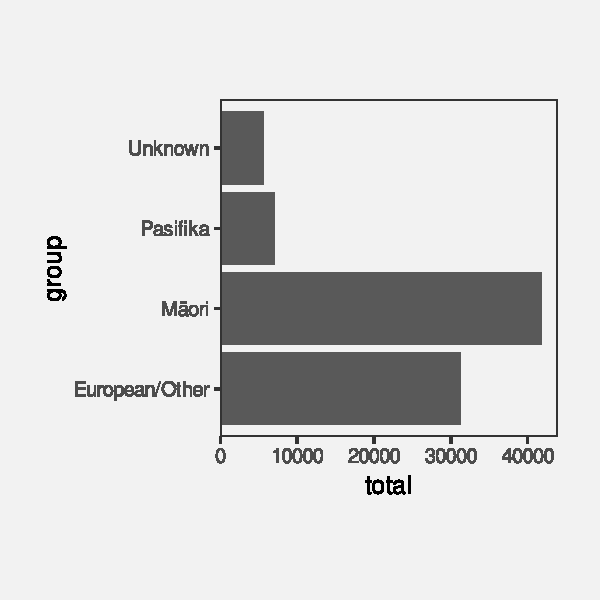
\includegraphics[width=1\linewidth,height=\textheight,keepaspectratio]{index_files/mediabag/congruence_files/figure-pdf/fig-more-is-more-1.pdf}

}

\subcaption{\label{fig-more-is-more-1}Bars.}

\end{minipage}%
%
\begin{minipage}{0.50\linewidth}

\centering{

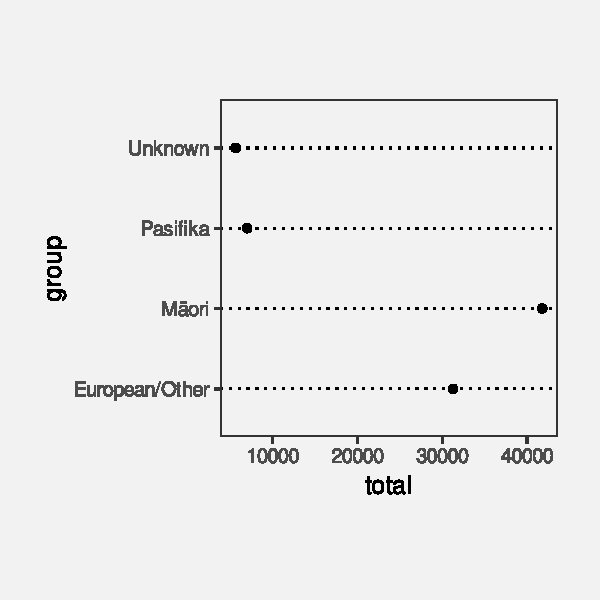
\includegraphics[width=1\linewidth,height=\textheight,keepaspectratio]{index_files/mediabag/congruence_files/figure-pdf/fig-more-is-more-2.pdf}

}

\subcaption{\label{fig-more-is-more-2}Dots.}

\end{minipage}%

\caption{\label{fig-more-is-more}A bar plot and a dot plot of the total
number of offenders for different ethnic groups.}

\end{figure}%

The Rugby World Cup is a competition that is held every four years, with
the first event taking place in 1987. We have data on the total number
of points that were scored and conceded in World Cup matches for Tier
One nations (the top 10 rugby-playing nations).
Table~\ref{tbl-rwc-all-time} shows these data.\footnote{Attribution to
  kaggle data set.}

\begin{longtable}[]{@{}lrrr@{}}

\caption{\label{tbl-rwc-all-time}A table of the total number of points
scored and conceded for Tier One nations in Rugby World Cup matches.}

\tabularnewline

\toprule\noalign{}
team & scored & conceded & diff \\
\midrule\noalign{}
\endhead
\bottomrule\noalign{}
\endlastfoot
Argentina & 535 & 719 & -184 \\
Australia & 779 & 594 & 185 \\
New Zealand & 1568 & 673 & 895 \\
South Africa & 609 & 441 & 168 \\
England & 695 & 624 & 71 \\
France & 716 & 674 & 42 \\
Ireland & 442 & 566 & -124 \\
Italy & 220 & 894 & -674 \\
Scotland & 305 & 571 & -266 \\
Wales & 497 & 610 & -113 \\

\end{longtable}

Another way that \textbf{length} can convey information more naturally
than \textbf{position} is visualising negative values. For example
Figure~\ref{fig-neg-bar} shows the total points differential (points
scored minus points conceded) for Tier One nations at Rugby World Cups
(see Table~\ref{tbl-rwc-all}). The \emph{direction} of the bars very
clearly indicates the change from positive points differential to
negative points differential.

\begin{figure}

\centering{

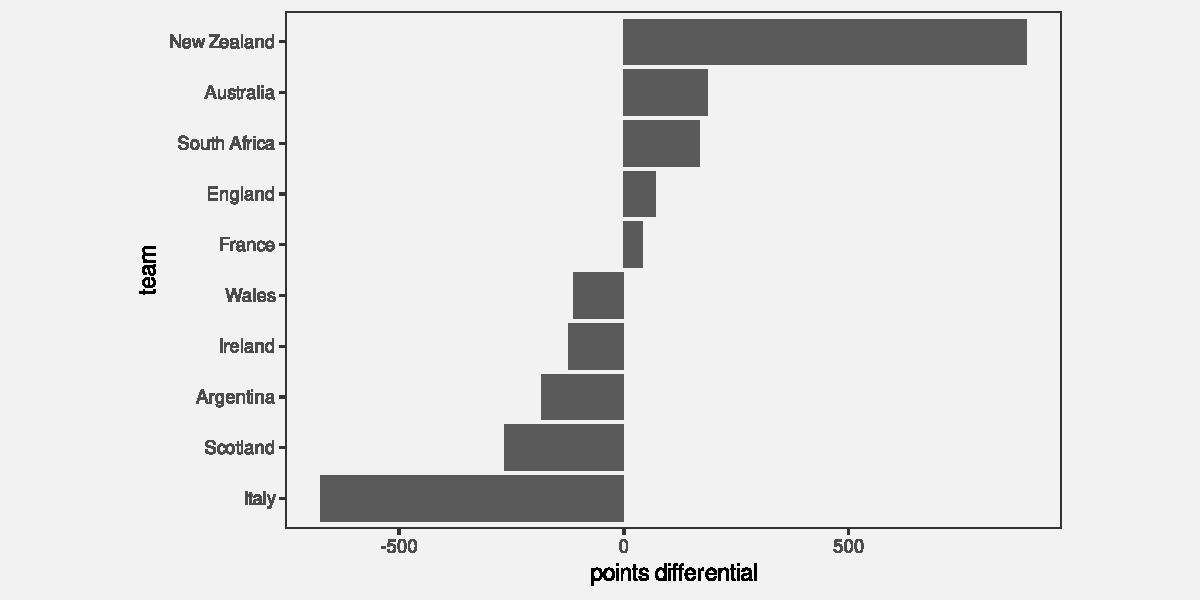
\includegraphics[width=1\linewidth,height=\textheight,keepaspectratio]{index_files/mediabag/congruence_files/figure-pdf/fig-neg-bar-1.pdf}

}

\caption{\label{fig-neg-bar}A bar plot of the total points differential
for Tier One nations at Rugby World Cups.}

\end{figure}%

By comparison, the change from positive to negative points differential
is much more abstract in a dot plot of the same data
(Figure~\ref{fig-neg-dot}).

\begin{figure}

\centering{

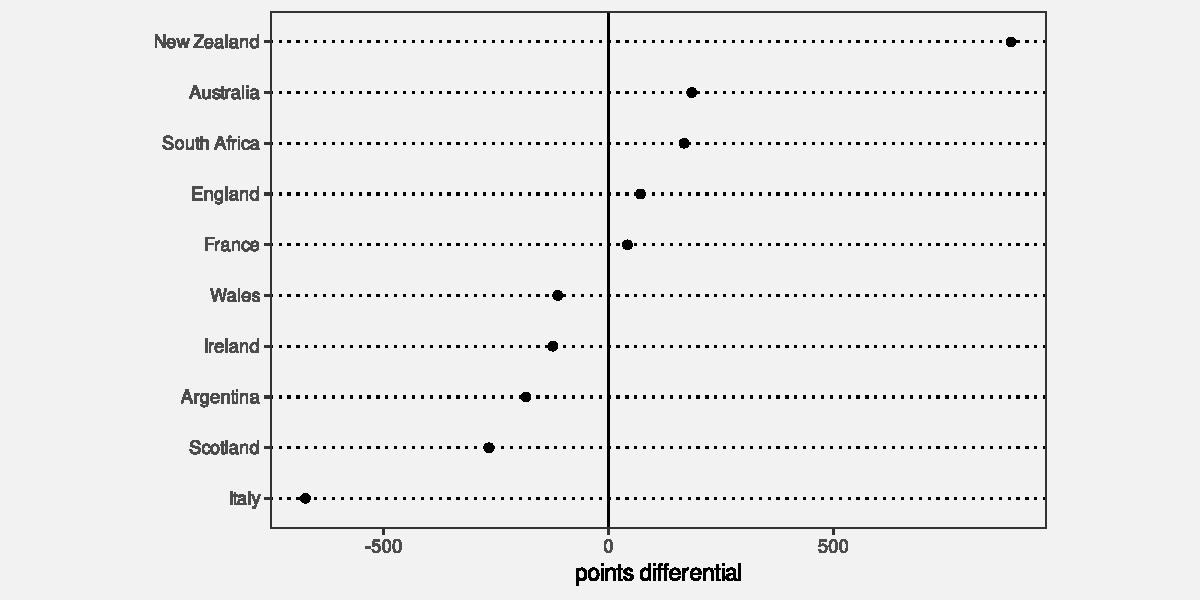
\includegraphics[width=1\linewidth,height=\textheight,keepaspectratio]{index_files/mediabag/congruence_files/figure-pdf/fig-neg-dot-1.pdf}

}

\caption{\label{fig-neg-dot}A dot plot of the total points differential
for Tier One nations at Rugby World Cups.}

\end{figure}%

\begin{quote}
One reason why bar plots are effective is because larger data values are
represented by larger data symbols.
\end{quote}

A more subtle effect can be seen in Figure~\ref{fig-bar-orientation},
which shows two different bar plots of the total number of offenders in
different ethnic groups. In this case, the vertical bars are more
natural for conveying count data like this because of the natural
correspondence with stacks of items.\footnote{horizontal bars
  (distances) versus vertical bars (amounts) look up Tversky and kosslyn
  OTOH, horizontal bars are more accurate than vertical bars (citation
  please!)}

\begin{figure}

\begin{minipage}{0.50\linewidth}

\centering{

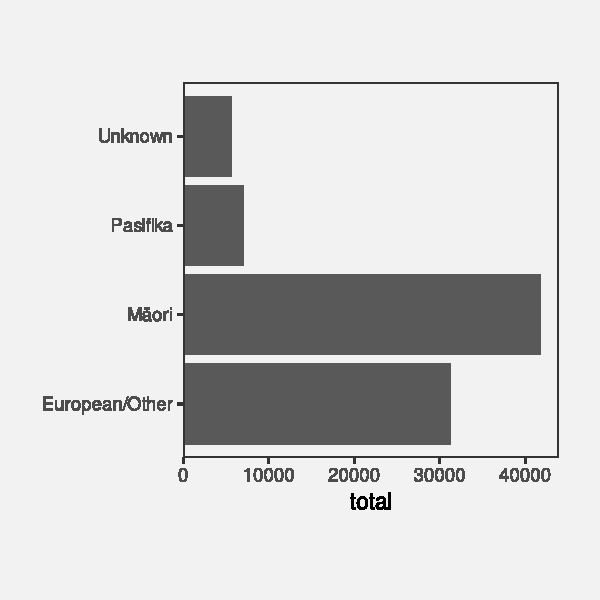
\includegraphics[width=1\linewidth,height=\textheight,keepaspectratio]{index_files/mediabag/congruence_files/figure-pdf/fig-bar-orientation-1.pdf}

}

\subcaption{\label{fig-bar-orientation-1}Horizontal bars.}

\end{minipage}%
%
\begin{minipage}{0.50\linewidth}

\centering{

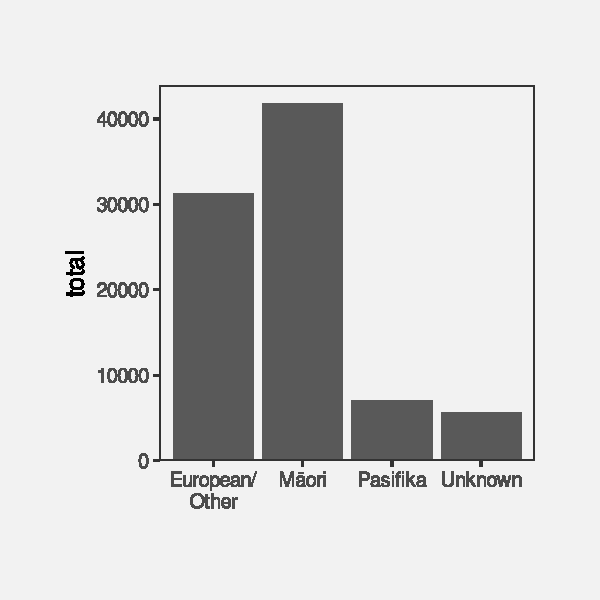
\includegraphics[width=1\linewidth,height=\textheight,keepaspectratio]{index_files/mediabag/congruence_files/figure-pdf/fig-bar-orientation-2.pdf}

}

\subcaption{\label{fig-bar-orientation-2}Vertical bars.}

\end{minipage}%

\caption{\label{fig-bar-orientation}Data visualisations of the number of
offenders from different ethnic groups.}

\end{figure}%

\section{Same is same}\label{sec-same-same}

In Section~\ref{sec-differences} we saw that the visual system is very
sensitive to \textbf{differences}, particularly when everything else
remains the \textbf{same}. This means that mapping \emph{changes} in
data values to \emph{changes} in data symbols will be effective because
the visual system will notice the differences in the data symbols. More
specifically, if a \textbf{visual feature} of a data symbol changes then
the visual system will notice that change. Furthermore, if a visual
feature of a data symbol changes while all other visual features of the
data symbol remain the \textbf{same}, the visual system will notice the
change more easily.\footnote{Sort of relates to Kosslyn's ``Principle of
  Informative Changes'' ``Graph Design for the Eye and Mind'' Kosslyn
  (2006)}

For example, in a bar plot like Figure~\ref{fig-bar}, the data symbols
are bars and only the \textbf{lengths} of the bars and the vertical
\textbf{positions} of the bars are different. The ``widths'' of the bars
and the \textbf{colours} of the bars remain the same.

\begin{quote}
Another reason why bar plots are effective is because the bars differ in
length, but are otherwise the same.
\end{quote}

\section{Dissonant mappings}\label{sec-dissonance}

The fact that \textbf{length} and \textbf{area} naturally convey amounts
means that care must be taken \emph{not} to confuse that association.
For example, Figure~\ref{fig-bar-not-zero} shows the number of times
each team entered the opposition's final third during a match at the
2023 Women's World Cup. The final third of the pitch is shown as darker
green regions, broken into five different zones, with a number of
entries for each zone and for each team represented by a line with an
arrow.

In Figure~\ref{fig-bar-not-zero}, longer lines correspond to a larger
number of entries. However, the bars start at the halfway line on the
pitch rather than at the final third of the pitch. This means that the
zero entries by South Africa into the second-from-right zone is
represented by a non-zero-length line. Apart from making comparisons of
the line lengths very inaccurate, this creates a confusing visual effect
because the viewer is expected to associate a non-zero length with a
value of zero.

\begin{figure}

\centering{

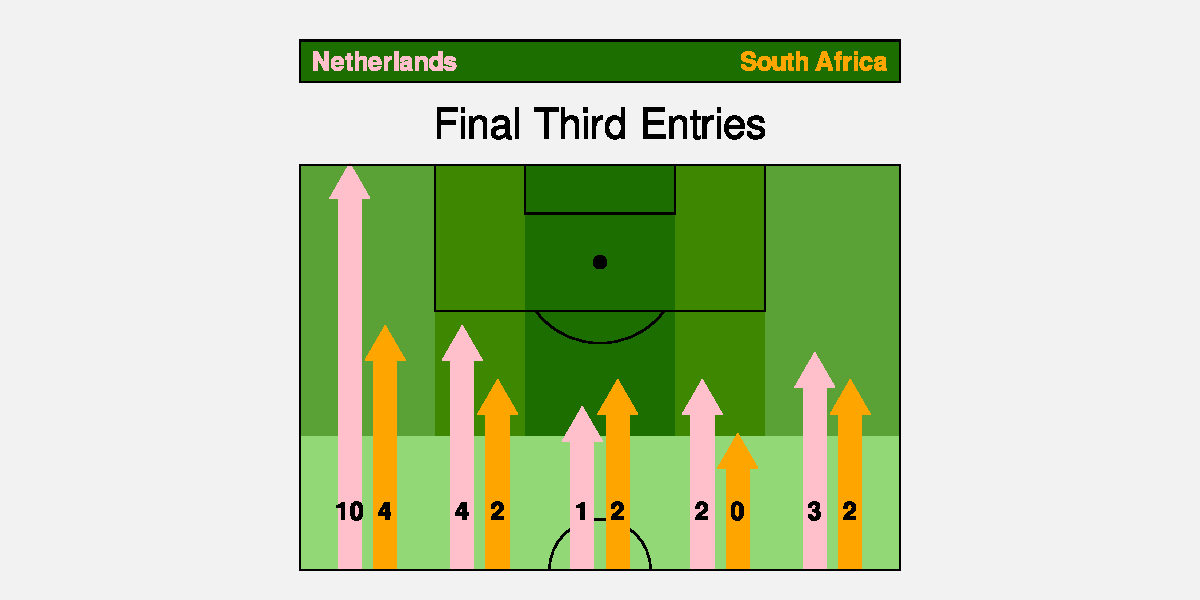
\includegraphics[width=1\linewidth,height=\textheight,keepaspectratio]{index_files/mediabag/congruence_files/figure-pdf/fig-bar-not-zero-1.pdf}

}

\caption[\label{fig-bar-not-zero}The number of times each team entered
the opposition's final third in the Women's World Cup match between the
Netherlands and South Africa.]{\label{fig-bar-not-zero}The number of times each team entered
the opposition's final third in the Women's World Cup match between the
Netherlands and South Africa.\footnotemark{}}

\end{figure}%
\footnotetext{This data visualisation is an
  adaptation of a graphic shown during television coverage of the match.}

For any example of \textbf{congruence}, where a visual feature naturally
corresponds to a property of the data, there is an opportunity for
\textbf{dissonance} if the visual feature is used inappropriately. We
can improve the effectiveness of a data visualisation by taking
advantage of visual congruence and we can reduce the effectiveness of a
data visualisation if we create visual dissonance.

If we fail to make our explicit encodings congruent with any implicit
encodings - if we create a \textbf{dissonant} mapping - we can make it
harder and more confusing to decode a data visualisation because there
is more than one possible decoding (Figure~\ref{fig-dissonant-decode}).

\begin{figure}

\centering{

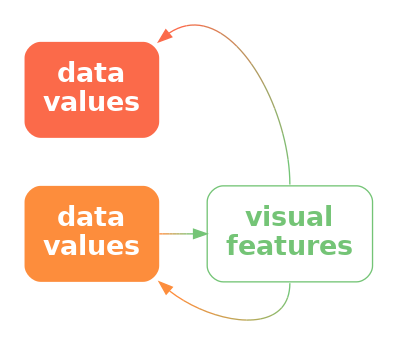
\includegraphics[scale=0.5]{Diagrams/dissonant-decode.png}

}

\caption{\label{fig-dissonant-decode}If we explicitly map data values to
visual features, but the visual features have an implicit mapping to
different data values, we can cause confusion and make it harder to
effectively decode data values from visual features.}

\end{figure}%

We saw in Section~\ref{sec-same-same} that we want to map differences in
data values to differences in visual features \emph{and} keep everything
else the same. Failing to follow that approach will make it harder to
perceive changes in the data values. However, a worse error, and another
source of visual dissonance arises if we change visual features
\emph{without} any underlying change in the data values.\footnote{``Graph
  Design for the Eye and Mind'' Kosslyn (2006) ``Principle of
  Informative Changes'' change in aesthetic where no change in data is
  BAD!}

Figure~\ref{fig-listener-cakes} shows a data visualisation of the
relative number of people aged over 100 for females versus males. There
are numerous problems with this data visualisation, but here we will
just focus on the horizontal \textbf{position} of the cake images. The
cakes for females are positioned to the left of the cakes for males,
which is acceptable because that difference in position reflects a
difference in the data---males versus females. However, within each
gender, the cakes are also staggered a small amount to the left then to
the right. This visual difference in the cake positions does not
correspond to any difference in the data values. We are tempted to seek
meaning from the the left-to-right staggering of the cakes when no
meaning exists.

\begin{figure}

\centering{

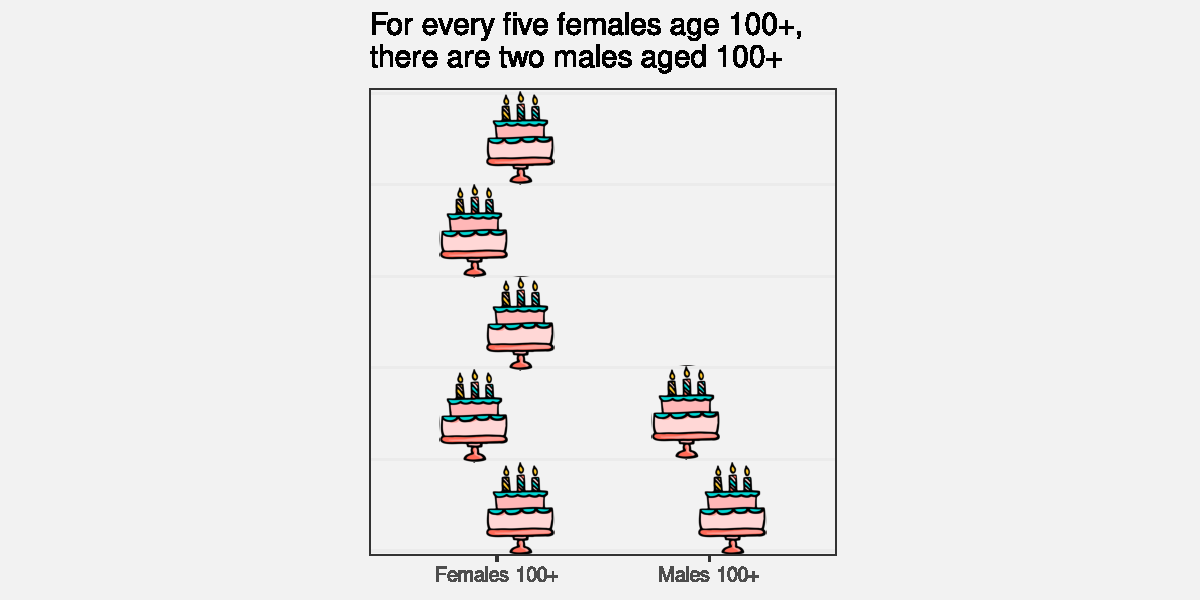
\includegraphics[width=1\linewidth,height=\textheight,keepaspectratio]{index_files/mediabag/congruence_files/figure-pdf/fig-listener-cakes-1.pdf}

}

\caption[\label{fig-listener-cakes}A data visualisation of the number of
females aged over 100 relative to the number of makes aged over
100.]{\label{fig-listener-cakes}A data visualisation of the number of
females aged over 100 relative to the number of makes aged over
100.\footnotemark{}}

\end{figure}%
\footnotetext{This plot is based on a data visualisation from the New
  Zealand Listener October 14-20 2023.}

\begin{quote}
A data visualisation is \emph{not} effective if it contains mappings
that are dissonant because that can cause distraction and slower and/or
incorrect \textbf{decoding} of data values from visual features.
\end{quote}

\section{Case study: Jittering}\label{case-study-jittering}

We have data on the number of points that were scored in every World Cup
match for Tier One nations (the top 10 rugby-playing nations).
Table~\ref{tbl-rwc-all} shows a sample of these data.\footnote{Attribution
  to kaggle data set.}

\begin{longtable}[]{@{}llr@{}}

\caption{\label{tbl-rwc-all}A table of the number of points scored by
Tier One nations in Rugby World Cup matches, along with the global
hemisphere of origin. Each row represents the points scored by one team
in one match. There are 294 rows in total, with just the first 6 rows
shown here.}

\tabularnewline

\toprule\noalign{}
team & hemisphere & scored \\
\midrule\noalign{}
\endhead
\bottomrule\noalign{}
\endlastfoot
Argentina & South & 8 \\
Argentina & South & 18 \\
Argentina & South & 13 \\
Argentina & South & 28 \\
Argentina & South & 10 \\
Argentina & South & 7 \\

\end{longtable}

Figure~\ref{fig-jitter} shows a scatterplot of the number of points
scored by teams from different hemispheres at Rugby World Cup matches
(see Table~\ref{tbl-rwc-all}). In this data visualisation, the data
symbols are dots, the number of points scored is encoded as the
horizontal \textbf{position} of the dots, and the hemisphere is encoded
as the vertical \textbf{position} of the dots.

To ameliorate the overlapping of data points, a random amount of
``jitter'' has been added the vertical position of the dots. The filled
interior of each dot is also semitransparent so that we can see where
points overlap.

\begin{figure}

\centering{

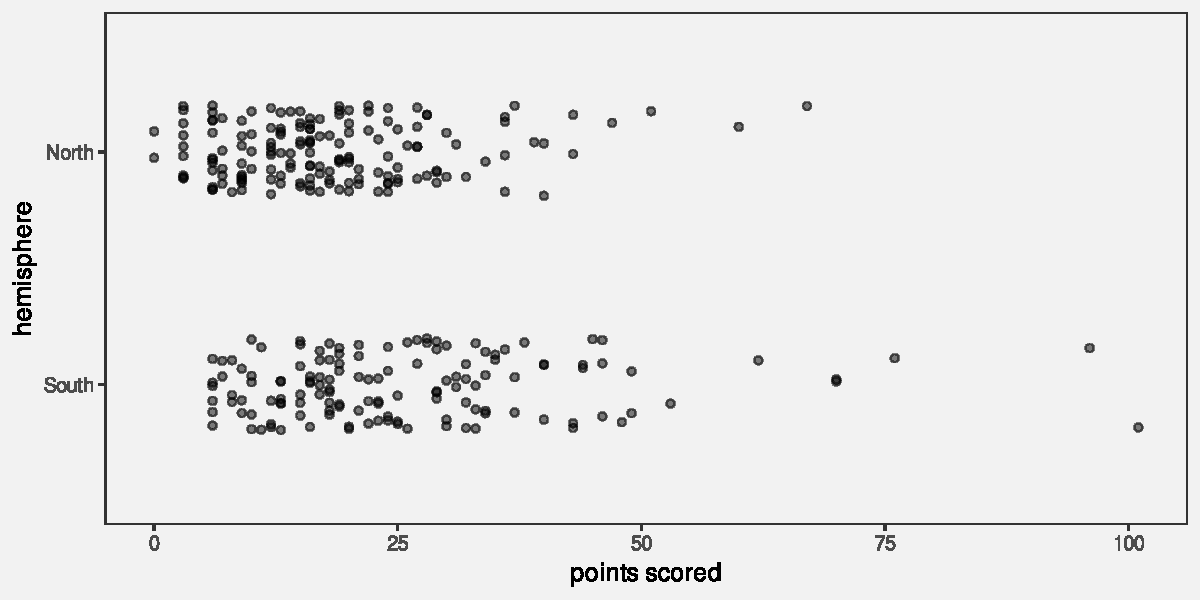
\includegraphics[width=1\linewidth,height=\textheight,keepaspectratio]{index_files/mediabag/congruence_files/figure-pdf/fig-jitter-1.pdf}

}

\caption{\label{fig-jitter}The number of points scored in Rugby World
Cup games by teams from the northern and southern hemispheres.}

\end{figure}%

The scatter plot in Figure~\ref{fig-jitter} is effective for
\textbf{decoding} to the number of points scored because each data value
is encoded as the horizontal position of a single data symbol.
Similarly, we can easily decode the hemisphere from each point. The
proximity of the data symbols from the same hemisphere means that it is
easy to perceive two ``rows'' of points.

On the other hand, the jittering means that there are visual differences
between the vertical positions of the dots, within the same hemisphere,
that do not correspond to any differences in data values. For example,
there are two dots representing matches where a team from the Northern
hemisphere scored zero points. The data values for these two dots are
identical (zero points scored and northern hemisphere), but they are
visually different. The randomness of the jittering may help to dilute
any temptation to seek meaning from the artificial visual difference,
but the addition of jittering may cause confusion.

\begin{quote}
Jittering data symbols is effective because it reduces the amount of
overlap amongst data symbols, but jittering may also reduce the
effectiveness of a data visualisation because it introduces visual
dissonance.
\end{quote}

\section{Summary}\label{summary-6}

The effectiveness of a data visualisation may depend on more than just
the accuracy and capacity of visual features.

A \textbf{congruent} mapping is one where data values are
\textbf{explicitly} encoded in a way that is consistent with an
\textbf{implicit} decoding of the visual feature.

Some data visualisations are effective because they are visually
congruent: data symbols that are larger for larger data values are more
effective; data symbols that only change if the data values change are
more effective.

A \textbf{dissonant} mapping is one where data values are
\textbf{explicitly} encoded in a way that is inconsistent with an
\textbf{implicit} decoding.

Some data visualisations are \emph{not} effective because they are
visually dissonant.

\begin{center}\rule{0.5\linewidth}{0.5pt}\end{center}

\theendnotes

\bookmarksetup{startatroot}

\chapter{Mapping Summaries}\label{sec-summaries}

In Chapter~\ref{sec-mapping-visual-features} we described a data
visualisation as a mapping that \textbf{encodes} data values as the
visual features of a data symbol (Figure~\ref{fig-visual-feature}). For
example, a bar plot, like Figure~\ref{fig-bar}, maps the total number of
youth offenders to the \textbf{lengths} of bars.

We also emphasised the importance of the \textbf{decoding} from visual
features to data values. For example, the effectiveness of the bar plot
in Figure~\ref{fig-bar} relies on our ability to accurately perceive the
lengths of the bars, particularly relative to each other.

In the simple scenario of a bar plot, the data values are counts (e.g.,
Table~\ref{tbl-crime-group-total}), which are encoded as the lengths of
bars, which in turn allows us to decode lengths to retrieve the counts
(Figure~\ref{fig-visual-feature-decode}). Each raw data value (count) is
mapped to the length of a bar.

In this section, we explore some data visualisations that are effective
because they encode \textbf{data summaries} instead of raw data
values.\footnote{MUST make reference to the Information Visualization
  Reference Model of Card et al (1999) that differentiates data
  transforms from visual mappings from view transforms (the last
  particularly for interactive graphics?)}

PLUS the design-centric extension by Wu and Chang (2024), which teases
out design-specific transforms as well (the data prep for a box plot
being a good example). These papers provide a formal basis for some of
the hand-waving that I do in this section, particularly on decoding to
data summaries rather than raw data.

Also ``Low-Level Components of Analytic Activity in Information
Visualization'' Amar et al (2005) Set of 10 data visualisation tasks I
like the way these all correspond to a numerical summary.

PLUS of course ``stats'' in Wilkinson GoG

\section{Box plots}\label{box-plots}

Figure~\ref{fig-boxplot} shows box plots of the number of points scored
by all teams at Rugby World Cup matches (Table~\ref{tbl-rwc-all}), with
a separate box plot for teams from different hemispheres. This is an
effective data visualisation for comparing the distributions of points
scored between hemispheres because we are able to easily see differences
between the median values of the countries (the thick vertical lines)
and differences between the interquartile ranges of the countries (the
horizontal rectangles). For example, we can see that the median points
scored by southern hemisphere teams is larger than the median for
northern hemisphere teams and the interquartile range of points scored
is also wider for southern hemisphere teams.

\begin{figure}

\centering{

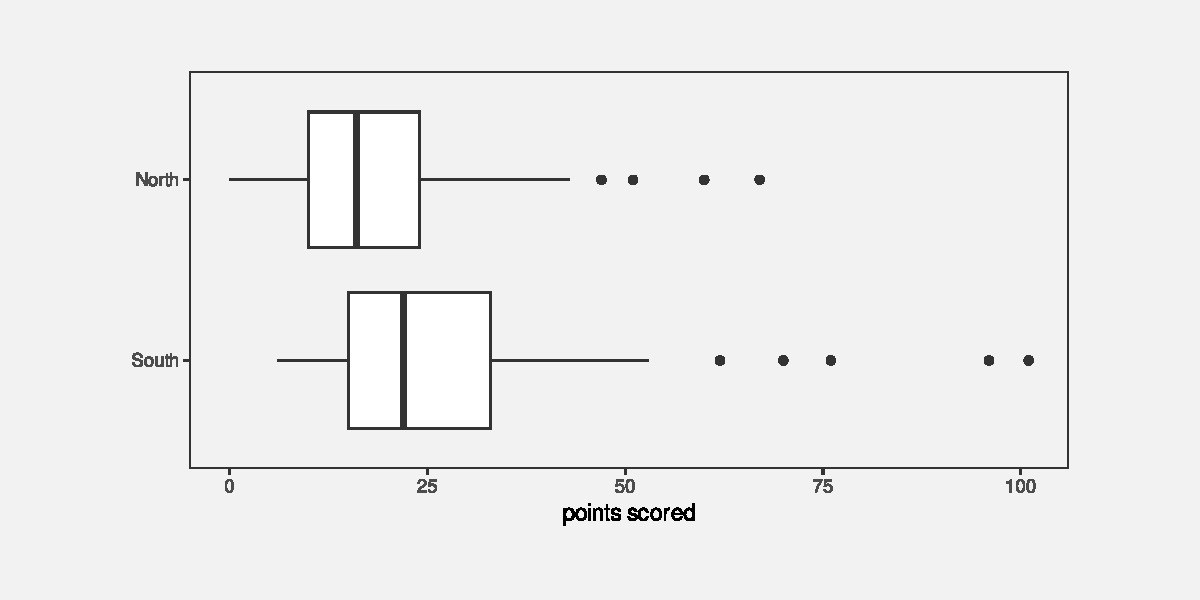
\includegraphics[width=1\linewidth,height=\textheight,keepaspectratio]{index_files/mediabag/summaries_files/figure-pdf/fig-boxplot-1.pdf}

}

\caption{\label{fig-boxplot}Box plots of the number of points scored in
all Rugby World Cup games by Tier One nations.}

\end{figure}%

Box plots are quite different from bar plots and dot plots because the
data symbol is a much more complicated shape: there is a vertical line
to represent the median, a rectangle to represent the interquartile
range (lower quartile to upper quartile), and horizontal lines to
represent the extremes of the data values, from the the quartiles to the
minimum and maximum values. Points are also included for ``outliers'' if
data values lie further than 1.5 times the interquartile range beyond
the quartiles.\footnote{Need to acknowledge that there are many
  variations, even on the simple box plot, e.g., notches, definitions of
  the box, let alone violin plots, etc.}

Another important difference with a box plot is that it maps
\textbf{data summaries}, rather than raw data values, to visual features
of the data symbol (Figure~\ref{fig-stat-vis-decode}). For example, the
median values are mapped to the horizontal \textbf{positions} of thick
vertical lines and the interquartile ranges are mapped to the
\textbf{lengths} of horizontal rectangles.

\begin{figure}

\centering{

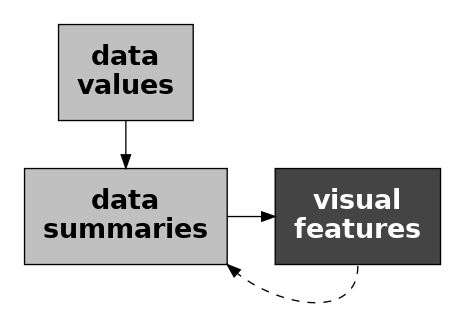
\includegraphics[scale=0.5]{Diagrams/stat-vis-decode.png}

}

\caption{\label{fig-stat-vis-decode}A data visualisation may encode data
summaries, rather than the raw data, as visual features. This is
effective for decoding the data summaries, but it is not effective for
decoding the raw data.}

\end{figure}%

To be explicit, the data values that are being \textbf{encoded} as
visual features in Figure~\ref{fig-boxplot} are \emph{not} the raw data
values in Table~\ref{tbl-rwc-all}; the values that are being encoded to
visual features in Figure~\ref{fig-boxplot} are the \textbf{data
summaries} shown in Table~\ref{tbl-rwc-all-stats}. These are the values
that we can \textbf{decode} from the boxplots in
Figure~\ref{fig-boxplot}.

\begin{longtable}[]{@{}lrrrrr@{}}

\caption{\label{tbl-rwc-all-stats}A table of the five-number summaries
for the number of points scored by Tier One nations in Rugby World Cup
matches, along with the country name. These data summaries are the
values that are mapped to visual features to produce the box plots in
Figure~\ref{fig-boxplot}.}

\tabularnewline

\toprule\noalign{}
& minimum & lower quartile & median & upper quartile & maximum \\
\midrule\noalign{}
\endhead
\bottomrule\noalign{}
\endlastfoot
South & 6 & 15 & 22 & 33 & 101 \\
North & 0 & 10 & 16 & 24 & 67 \\

\end{longtable}

Figure~\ref{fig-boxplot} is effective for allowing us to compare
summaries like the medians between different hemispheres because,
although the box plot data symbol is relatively complicated, a box plot
still just encodes the data summaries to simple visual features. We know
from Chapter~\ref{sec-mapping-visual-features} that \textbf{position}
and \textbf{length} are effective for \textbf{decoding} the data
summaries from the visual features (Figure~\ref{fig-stat-vis-decode}).

Notice how, even though Table~\ref{tbl-rwc-all-stats} contains very few
values, it is much easier to perceive the differences between the two
rows of values using the data visualisation in Figure~\ref{fig-boxplot}
rather than the table of values in Table~\ref{tbl-rwc-all-stats}. Once
again, we can see the power of mapping values to basic visual features.
The only differences from previous sections is that we are mapping
\textbf{data summaries} rather than raw data values and we are mapping
to the visual features of a more complicated data symbol.

\begin{quote}
A box plot is effective at conveying information about the distribution
of data values because it maps \textbf{data summaries} about the
distribution, like the median and interquartile range, to basic visual
features.
\end{quote}

\section{Visual summaries}\label{sec-visual-summaries}

Figure~\ref{fig-rwc-dotplot} shows stacked dot plots of the number of
points scored by countries from the different hemispheres in Rugby World
Cup matches.\footnote{Wilkinson (1999)} This data visualisation uses the
same data as Figure~\ref{fig-boxplot}, but it maps raw data values
rather than data summaries and it uses much simpler data symbols (data
points). This data visualisation encodes the number of points scored
maps as the horizontal \textbf{position} of a data point and it encodes
the hemisphere as the vertical \textbf{position} of a data point.

Because this data visualisation encodes raw data values as visual
features, it is possible to decode raw data values from the visual
features (Figure~\ref{fig-visual-feature-decode}). For example, it is
possible to see that the lowest score (zero points) for a northern
hemisphere team ocurred twice. It is also possible to see that there are
scores that have never occurred in any matches: 1, 2, 4, and 5. These
features are not visible in the boxplots in Figure~\ref{fig-boxplot}.

\begin{figure}

\centering{

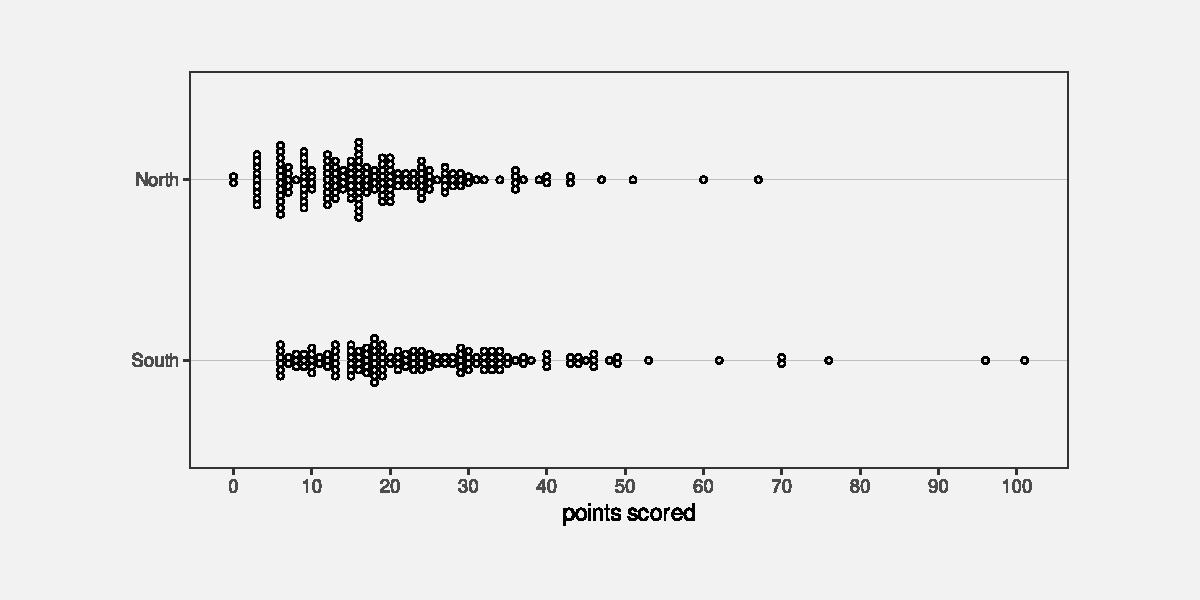
\includegraphics[width=1\linewidth,height=\textheight,keepaspectratio]{index_files/mediabag/summaries_files/figure-pdf/fig-rwc-dotplot-1.pdf}

}

\caption{\label{fig-rwc-dotplot}Stacked dotplots of the number of points
scored by Tier One nations at Rugby World Cup matches.}

\end{figure}%

The fact that we can decode raw data values from a dot plot is not news.
That is easy because we have encoded raw data values as accurate visual
features (see Section~\ref{sec-dot-plots}). However,
Figure~\ref{fig-rwc-dotplot} also demonstrates that, in addition to
decoding raw data values from visual features, our visual system allows
us to decode \textbf{data summaries} from visual features.

For example, we can see that the southern hemisphere teams score
slightly more points on average than the northern hemisphere teams; the
data symbols for southern-hemisphere teams appear shifted to the right
of the data symbols for northern-hemisphere teams. In other words, we
can perceive \textbf{visual summaries}; we can perceive \textbf{data
summaries} from collections of visual features. For example, we can
visually average the \textbf{positions} of the data points.

In Figure~\ref{fig-rwc-dotplot}, we have encoded raw data values as
visual features, which has enabled us to decode raw data values from
individual visual features. In addition, \textbf{visual summaries} of
the visual features enable us to decode \textbf{data summaries} from
collections of visual features
(Figure~\ref{fig-data-vis-stat-decode}).\footnote{Need some references
  to articles about ensembles in data vis lit (ideally NOT the scatter
  plot one cos want to use that later for scatter plots). ALSO must
  relate this to Gestalt section in visual model ?}

\begin{figure}

\centering{

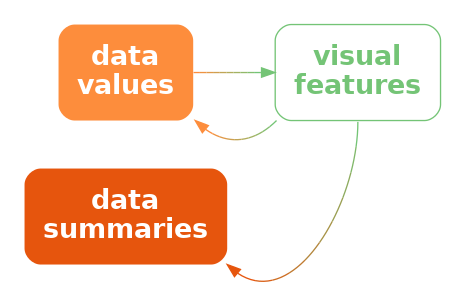
\includegraphics[scale=0.5]{Diagrams/data-vis-stat-decode.png}

}

\caption{\label{fig-data-vis-stat-decode}A data visualisation that
encodes data values as visual features allows us to decode data values,
but it may \emph{also} allow us to decode summaries of the data, such as
measures of central tendency or variability.}

\end{figure}%

\begin{quote}
A dot plot is effective not just for perceiving raw data values, but
also for perceving data summaries like clusters and outliers, and
central tendency and spread.
\end{quote}

\section{Case study: Histograms}\label{case-study-histograms}

Figure~\ref{fig-hist} shows a histogram of the number of points scored
by Tier One nations at the Rugby World Cups (Table~\ref{tbl-rwc-all}). A
histogram is similar to a box plot in two ways: a histogram is a data
visualisation that can be used to convey the distribution of a variable;
and a histogram is a data visualisation that maps data summaries, rather
than raw values, to visual features (Figure~\ref{fig-stat-vis-decode}).

However, a histogram differs from a box plot in two main ways: the data
symbol for a histogram is simpler than a box plot, because it consists
of just rectangles or bars; and the data summaries for a histogram are
more complicated than those for a box plot.

The raw data values for the histogram in Figure~\ref{fig-hist} are the
points scored in each game by each country (Table~\ref{tbl-rwc-all}). To
get the data summaries for the histogram, the raw data values are
binned; we break the range of the data into equal-sized intervals and
count how many data values lie in each interval. The centre of each
interval is then encoded as the horizontal \textbf{position} of a bar
and the count of data values in each interval is encoded as the
\textbf{length} of a bar.

\begin{figure}

\centering{

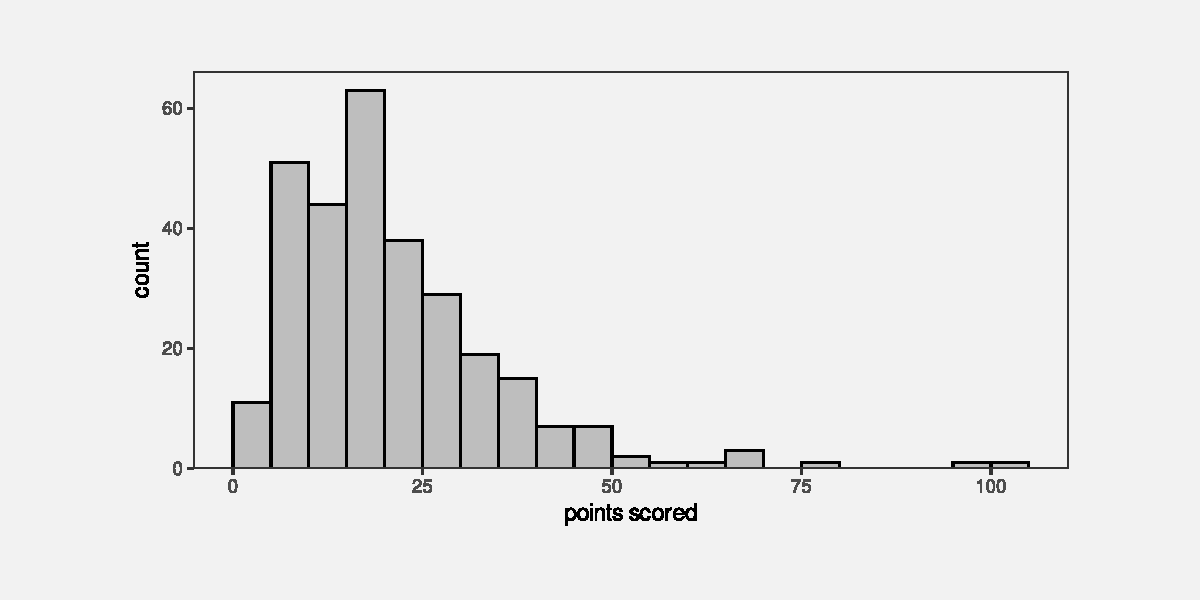
\includegraphics[width=1\linewidth,height=\textheight,keepaspectratio]{index_files/mediabag/summaries_files/figure-pdf/fig-hist-1.pdf}

}

\caption{\label{fig-hist}A histogram of the points scored per game by
Tier One nations at Rugby World Cups.}

\end{figure}%

To be explicit, the values that are being mapped to visual features in
Figure~\ref{fig-hist} are not raw data values, but data
summaries---intervals and counts---as shown in
Table~\ref{tbl-hist-stats}.

\begin{longtable}[]{@{}
  >{\raggedright\arraybackslash}p{(\linewidth - 42\tabcolsep) * \real{0.0667}}
  >{\raggedleft\arraybackslash}p{(\linewidth - 42\tabcolsep) * \real{0.0296}}
  >{\raggedleft\arraybackslash}p{(\linewidth - 42\tabcolsep) * \real{0.0370}}
  >{\raggedleft\arraybackslash}p{(\linewidth - 42\tabcolsep) * \real{0.0444}}
  >{\raggedleft\arraybackslash}p{(\linewidth - 42\tabcolsep) * \real{0.0444}}
  >{\raggedleft\arraybackslash}p{(\linewidth - 42\tabcolsep) * \real{0.0444}}
  >{\raggedleft\arraybackslash}p{(\linewidth - 42\tabcolsep) * \real{0.0444}}
  >{\raggedleft\arraybackslash}p{(\linewidth - 42\tabcolsep) * \real{0.0444}}
  >{\raggedleft\arraybackslash}p{(\linewidth - 42\tabcolsep) * \real{0.0444}}
  >{\raggedleft\arraybackslash}p{(\linewidth - 42\tabcolsep) * \real{0.0444}}
  >{\raggedleft\arraybackslash}p{(\linewidth - 42\tabcolsep) * \real{0.0444}}
  >{\raggedleft\arraybackslash}p{(\linewidth - 42\tabcolsep) * \real{0.0444}}
  >{\raggedleft\arraybackslash}p{(\linewidth - 42\tabcolsep) * \real{0.0444}}
  >{\raggedleft\arraybackslash}p{(\linewidth - 42\tabcolsep) * \real{0.0444}}
  >{\raggedleft\arraybackslash}p{(\linewidth - 42\tabcolsep) * \real{0.0444}}
  >{\raggedleft\arraybackslash}p{(\linewidth - 42\tabcolsep) * \real{0.0444}}
  >{\raggedleft\arraybackslash}p{(\linewidth - 42\tabcolsep) * \real{0.0444}}
  >{\raggedleft\arraybackslash}p{(\linewidth - 42\tabcolsep) * \real{0.0444}}
  >{\raggedleft\arraybackslash}p{(\linewidth - 42\tabcolsep) * \real{0.0444}}
  >{\raggedleft\arraybackslash}p{(\linewidth - 42\tabcolsep) * \real{0.0444}}
  >{\raggedleft\arraybackslash}p{(\linewidth - 42\tabcolsep) * \real{0.0519}}
  >{\raggedleft\arraybackslash}p{(\linewidth - 42\tabcolsep) * \real{0.0593}}@{}}

\caption{\label{tbl-hist-stats}A table of intervals the cover the range
of the number of points scored by Tier One nations in Rugby World Cup
matches, along with the count of the number of points scored that fall
within each interval. These data summaries are the values that are
mapped to visual features to produce the histogram in
Figure~\ref{fig-boxplot}.}

\tabularnewline

\toprule\noalign{}
\endhead
\bottomrule\noalign{}
\endlastfoot
interval & 0-5 & 5-10 & 10-15 & 15-20 & 20-25 & 25-30 & 30-35 & 35-40 &
40-45 & 45-50 & 50-55 & 55-60 & 60-65 & 65-70 & 70-75 & 75-80 & 80-85 &
85-90 & 90-95 & 95-100 & 100-105 \\
count & 11 & 51 & 44 & 63 & 38 & 29 & 19 & 15 & 7 & 7 & 2 & 1 & 1 & 3 &
0 & 1 & 0 & 0 & 0 & 1 & 1 \\

\end{longtable}

As with a box plot, encoding data summaries as accurate visual features
means that we can easily decode data summaries from the visual features.
For a histogram, this means that we can easily compare the lengths of
the bars, which means we can easily compare the relative counts of data
values within each interval. For example, the longest bars represent the
intervals that contain a relatively large count of data values, which
tells us about the mode of the data (or the number of modes in the
data). In Figure~\ref{fig-hist} we can see that the largest number of
data values occur around 15 to 20 points and we can see that the number
of data values in each interval drops more rapidly above the highest bar
than below the highest bar. The latter tells us about the spread and/or
skewness of the data.

\begin{quote}
A histogram is effective at conveying information about the distribution
of data values because it maps data summaries to basic visual features
and those data summaries can be compared to provide information about
the distribution of the data.
\end{quote}

\section{The dangers of summaries}\label{sec-summary-caveats}

The benefit of a data visualisation that encodes \textbf{data summaries}
as visual features is that it allows us to decode data summaries very
easily. For example, although we can perceive a general idea of central
tendency from the dots in Figure~\ref{fig-rwc-dotplot} (see
Section~\ref{sec-visual-summaries}), it is much easier and more accurate
to perceive median values from the thick vertical lines in
Figure~\ref{fig-boxplot}.

The flipside is that a data visualisation that encodes \textbf{data
summaries} as visual features is \emph{not} effective for decoding raw
data values. For example, we cannot see from the box plot in
Figure~\ref{fig-boxplot} that the scores 1, 2, 4, and 5 never occurred,
while this is clear from Figure~\ref{fig-rwc-dotplot} because the dot
plot does map the raw data values to data symbols.

\begin{quote}
Box plots and histograms are \emph{not} effective at conveying raw data
values because they do not map raw data values to data symbols.
\end{quote}

Another point to consider with a data visualisation that is based on
data summaries is whether the data summaries provide reasonable
summaries of the data.\footnote{Cite Anscombe's quartet and the dinosaur
  one.} For example, Figure~\ref{fig-boxplot-concede} shows box plots of
the number of points \emph{conceded} by each team in Rugby World Cup
games. The box plot for southern hemisphere teams suggests a unimodal
distribution with a slight right skew.

\begin{figure}

\centering{

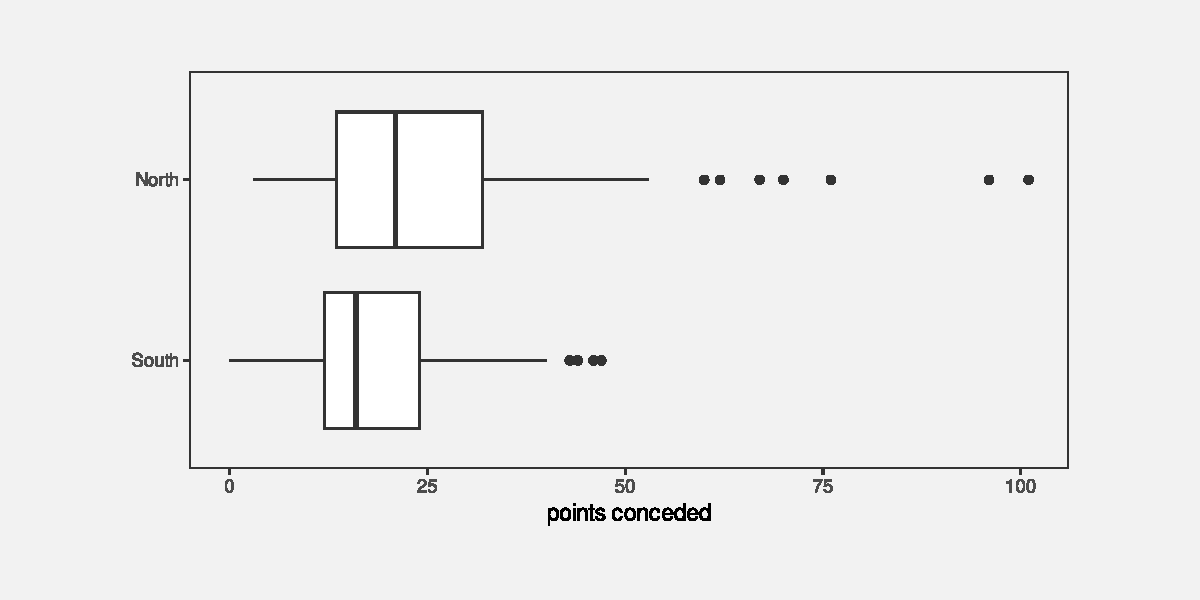
\includegraphics[width=1\linewidth,height=\textheight,keepaspectratio]{index_files/mediabag/summaries_files/figure-pdf/fig-boxplot-concede-1.pdf}

}

\caption{\label{fig-boxplot-concede}Box plots of the number of points
conceded in all Rugby World Cup games by Tier One nations.}

\end{figure}%

However, the dot plots in Figure~\ref{fig-rwc-dotplot-concede} tell a
different story. This data visualisation shows some evidence that the
number of points conceded by southern-hemisphere teams may be bimodal,
with some teams only conceding very few points (0, 3, or 6) in a number
of games. The data summaries for a box plot assume a unimodal
distribution, so a box plot will only ever tell a unimodal story, and
that is only reasonable if the data are unimodal.

\begin{figure}

\centering{

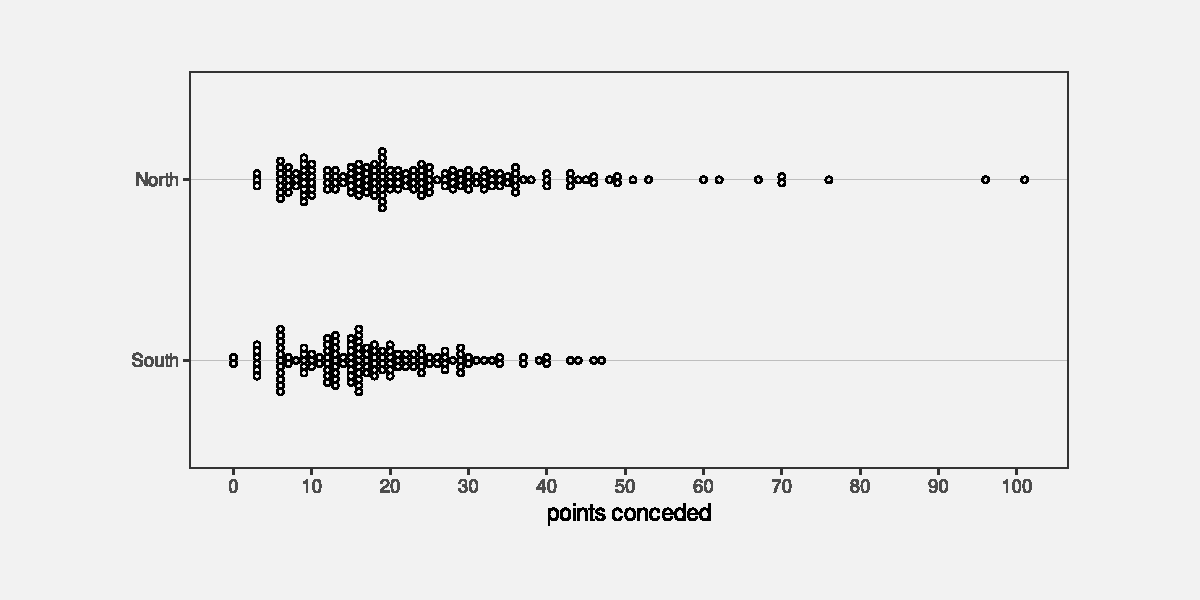
\includegraphics[width=1\linewidth,height=\textheight,keepaspectratio]{index_files/mediabag/summaries_files/figure-pdf/fig-rwc-dotplot-concede-1.pdf}

}

\caption{\label{fig-rwc-dotplot-concede}Stacked dotplots of the number
of points conceded by Tier One nations at Rugby World Cup matches.}

\end{figure}%

\begin{quote}
A data visualisation that is based on data summaries can only be
effective if the data summaries are sensible summaries of the data.
\end{quote}

A box plot is \emph{not} effective if a five-number summary is not a
sensible summary of the data values.

A further complication arises with histograms because we have to
\emph{choose} the intervals that are used to calculate the data
summaries and that choice can have a large influence on the data
summaries. For example, Figure~\ref{fig-hist-thin} shows a histogram of
the same data that we used for Figure~\ref{fig-hist}, but with a greater
number of narrower intervals. This visualisation tells a slightly
different story than Figure~\ref{fig-hist}. The most common score is now
6 points (rather than between 15 and 20 points) and we see features like
gaps at 1, 2, 4, and 5 points and a stronger suggestion of bimodality.
There are also point totals that appear strangely low, like 11 and 14.

Unlike a box plot, where the data summaries are essentially fixed
calculations, for a histogram we get to choose the data summaries to
some extent, which means that we get to choose the story that the data
visualisation tells. Figure~\ref{fig-hist} tells a simpler story, but
Figure~\ref{fig-hist-thin} tells a story that includes some important
details.

When using a histogram for exploring a data set, it is a good idea to
try out more than one choice of intervals in order to avoid missing an
important story. When using a histogram to present a story about a data
set, there is a responsibility to present a story that does not exclude
important details.

\begin{figure}

\centering{

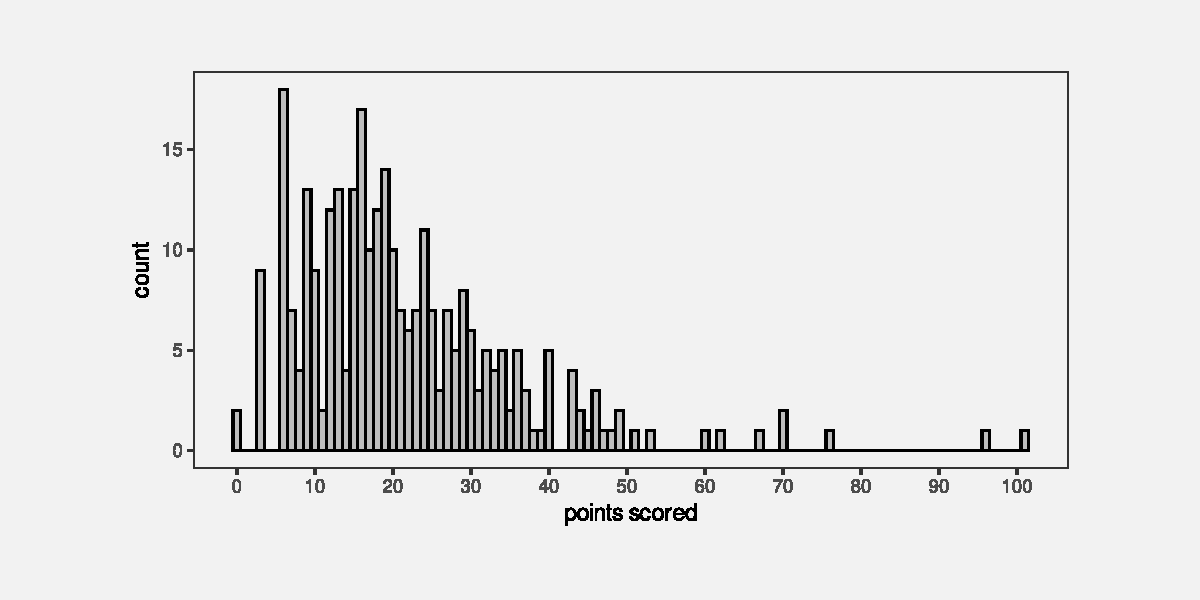
\includegraphics[width=1\linewidth,height=\textheight,keepaspectratio]{index_files/mediabag/summaries_files/figure-pdf/fig-hist-thin-1.pdf}

}

\caption{\label{fig-hist-thin}A histogram of the points scored per game
by Tier One nations at Rugby World Cups. This histogram uses the same
data as Figure~\ref{fig-hist}, but bins the data using narrower
intervals.}

\end{figure}%

\section{Case study: How charts lie}\label{case-study-how-charts-lie}

In this document, we assume that the purpose of a data visualisation is
to faithfully and honestly encode data values and the goal is to produce
a data visualisation that provides the most effective decoding of visual
features (see Section~\ref{sec-scope}).

Nevertheless, less honest representations of data can also be described
in terms of mappings, particularly mappings of data summaries.

For example, \ldots{} Figure~\ref{fig-bars-at-zero}\footnote{This is a
  reproduction of a chart from Alberto Cairo's ``How Charts Lie''
  (p12-13), which itself was a reproduction of a chart shown by Fox
  News. (plus mention other classic how charts lie books like Huff's How
  to Lie With Statistics ?) Also link to Wilke's Principle of
  Proportional Ink?} This does not encode the raw data as the lengths of
the bars, but the raw data - 34. The top rate under Obama would be 39.6.
Also does not help that the y-axis scale is not shown!

\begin{figure}

\centering{

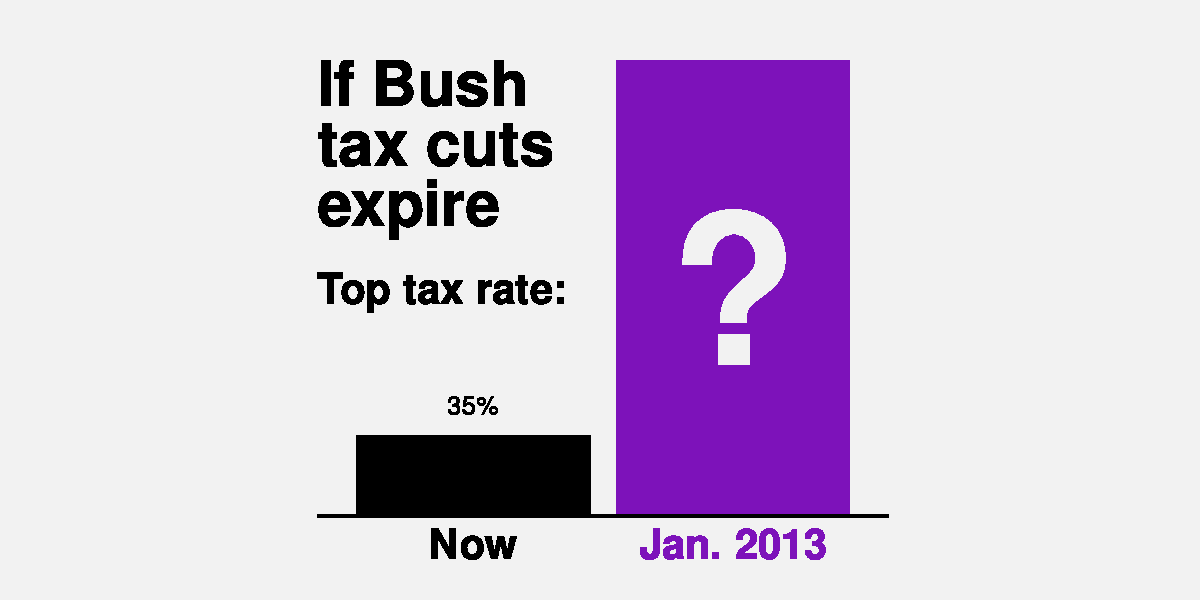
\includegraphics[width=1\linewidth,height=\textheight,keepaspectratio]{index_files/mediabag/summaries_files/figure-pdf/fig-bars-at-zero-1.pdf}

}

\caption{\label{fig-bars-at-zero}A bar plot of the increase in the top
tax rate in the United States of America from President George W. Bush
to President Barack Obama.}

\end{figure}%

A data visualisation that encodes distorted data or one that leaves out
an important subset of the data is encoding unhelpful values to visual
features. It is only then possible to decode from visual features to
unhelpful data values.

\begin{figure}

\centering{

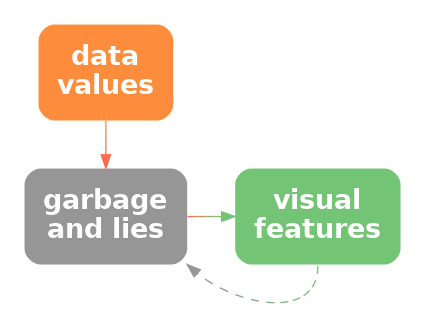
\includegraphics[scale=0.5]{Diagrams/lie-vis-decode.png}

}

\caption{\label{fig-lie-vis-decode}A data visualisation may map an
unrepresentative or ``cooked'' version of the data, rather than the raw
data, to visual features. Visual decoding leads back to the lies rather
than the real data.}

\end{figure}%

\section{Simplification}\label{simplification}

deliberately losing information (e.g., luminance scale for quant)

``Why Shouldn't All Charts Be Scatter Plots? Beyond Precision-Driven
Visualizations'' Bertini et al (2021) Claims that ordinal comparisons
more common in practice than quantitative comparisons (?)

This nice quote \ldots{}

\begin{quote}
Graphics are for comparison - comparison of one kind or another - not
for access to individual amounts. (Tukey 1993)
\end{quote}

\ldots{} points out that reading individual values off a plot is not
usually the point of a data vis, though it is still a precursor to
making a comparison. In some ways, ordinal comparisons are more
important than interval or ratio?

\section{Case study: Heatmaps}\label{case-study-heatmaps}

Heatmaps are a common way of representing three-dimensional data where
two of the data variables are either qualitative or have been measured
on a regular grid. The latter two variables naturally map to horizontal
and vertical \textbf{position} to produce an array of rectangles, while
the third variable maps to \textbf{colour} (see
Figure~\ref{fig-crime-heatmap}).

The mappings from data values to visual features for a heatmap are
\ldots{}

colour is not quant but can convey trends

using luminance for quant, but not trying for accurate decoding of
individual data values, BUT mention effectiveness of luminance in
heatmap for ensemble perception of regions?

get contrast effect but again not typically trying to match cells

get regions/shapes of colour =\textgreater{} higher-level structures

talk about colour palettes that have deliberate colour boundaries to
emphasise structure - combination of order and category

\section{Cognitive load}\label{cognitive-load}

On page 46 of his book ``How the World Really Works'' (Smil 2022),
Vaclav Smil writes that:

``rising food production reduced the malnutrition rate from 2 in 3
people in 1950 to 1 in 11 by 2019''

In order to comprehend the change in malnutrition rate, we are required
to compare ``2 in 3'' to ``1 in 11''. This requires mental effort to
calculate the ratios or fractions and then compare them. It is easier to
compare the rates if we hold the denominator constant, comparing ``2 in
3'' to ``2 in 22''. It is easier still if we calculate the fractions,
comparing 0.667 to 0.091. And it is easier still to compare those
fractions visually (Figure~\ref{fig-cog-load}).

\begin{figure}

\centering{

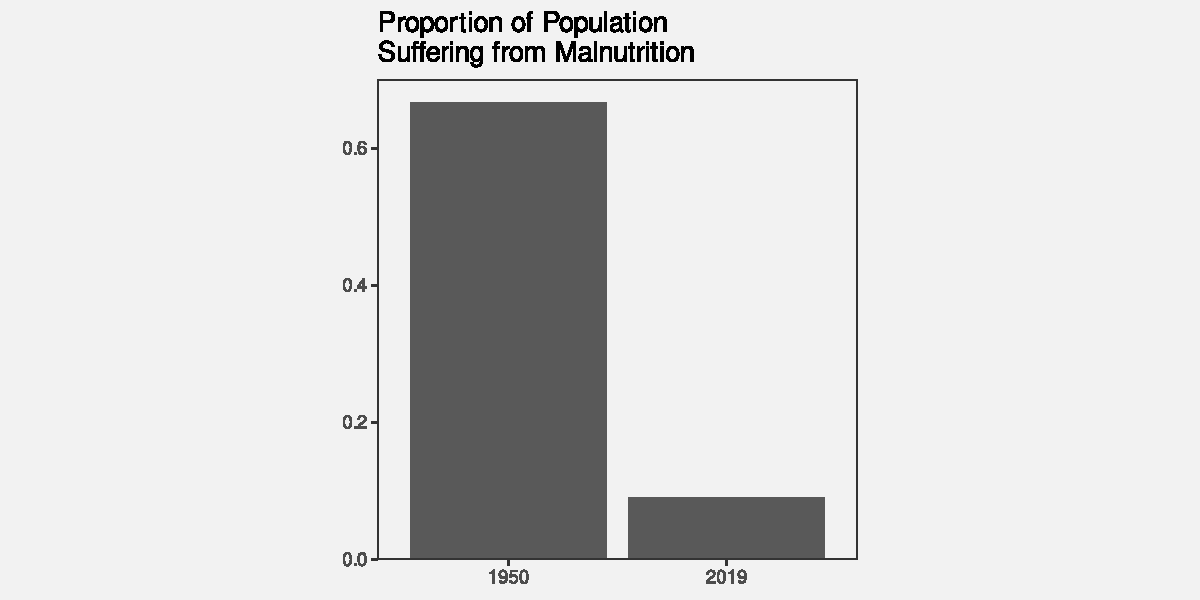
\includegraphics[width=1\linewidth,height=\textheight,keepaspectratio]{index_files/mediabag/summaries_files/figure-pdf/fig-cog-load-1.pdf}

}

\caption{\label{fig-cog-load}A bar plot comparing two fractions.}

\end{figure}%

The point is that we can reduce the cognitive load that is required of
the viewer if we make the mental calculations that are required easier.
We can reduce the cognitive load further if we present the results of
the calculation directly and even further if we encode the results of
the calculation as simple visual features.

Conversely, we can add to the cognitive load if we make the visual
calculations harder. For example, Figure~\ref{fig-cog-load-hi} shows a
bar plot of the original ``2 in 3'' versus ``1 in 11'' data values. We
now need to perceive the proportion of blue bars relative to red bars
and compare those proportions, which is clearly more work than just
comparing the two bars in Figure~\ref{fig-cog-load}.

\begin{figure}

\centering{

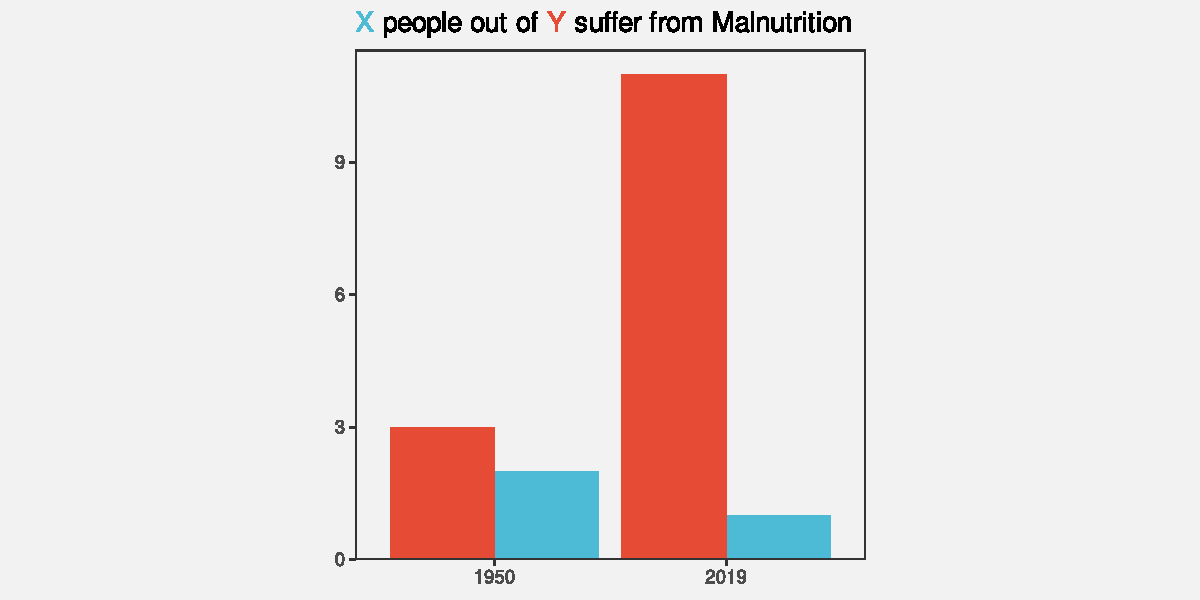
\includegraphics[width=1\linewidth,height=\textheight,keepaspectratio]{index_files/mediabag/summaries_files/figure-pdf/fig-cog-load-hi-1.pdf}

}

\caption{\label{fig-cog-load-hi}A bar plot comparing two fractions.}

\end{figure}%

We ideally want to present data in a way that imposes the least
cognitive load on the viewer. In terms of Section~\ref{sec-tasks}, we
want to present the viewer with simple \textbf{visual tasks}.

The best data visualisation will be different for different questions of
interest, but if the question of interest involves comparing data
summaries, then one way that we can make the viewer's life easier is by
calculating summaries of the data and encoding data summaries as visual
features, rather than encoding raw data values and asking the viewer to
perform visual summaries.

\begin{quote}
It is possible in some cases to rely on visual summaries, but we need to
be careful not to set a visual task that requires too much mental
effort.
\end{quote}

\section{Summary}\label{summary-7}

Data summaries, such as measures of central tendency, measures of
variability, and tables of counts, provide information about the
distribution of a set of data values.

Some data visualisations, like box plots and histograms, are effective
because they map \textbf{data summaries} to visual features. This makes
it easy to perceive and compare data summaries.

Care must be taken to use data summaries that appropriately summarise
the data values.

When we map raw data values to visual features, like in a dot plot, the
perception of individual visual features allows us to perceive and
compare raw data values, but, in addition, \textbf{visual summaries} of
\emph{collections} of visual features allow us to perceive and compare
data summaries.

A box plot that maps data summaries to visual features is more effective
for perceiving data summaries than a dot plot that relies on visual
summaries. However, a dot plot is more effective for perceiving raw data
values.

\begin{center}\rule{0.5\linewidth}{0.5pt}\end{center}

\theendnotes

\bookmarksetup{startatroot}

\chapter{Combining Mappings}\label{combining-mappings}

Most data visualisations involve more than one data variable. For
example, the bar plot in Figure~\ref{fig-bar} involves data on the
\textbf{ethnic group} of offenders and data on the \textbf{count} of
offenders in each ethnic group.

In Figure~\ref{fig-bar}, each data value is mapped to a \textbf{visual
feature} of a data symbol (Figure~\ref{fig-visual-feature}). For
example, the ethnic group is encoded as the vertical \textbf{position}
of the bars and the count of offenders is encoded as the \textbf{length}
of the bars.

We have so far only looked at mappings from data values to visual
features in isolation. For example, we know that the mapping from ethnic
group to position is effective because position is appropriate for
qualitative data and position has sufficient capacity to differentiate
between four ethnic groups. We also know that mapping the count of
offenders to length is effective because length is appropriate for
quantitative data and length provides an accurate decoding. Furthermore,
the lengths of the bars are all aligned (they have a common baseline)
and the bars only differ in ways that reflect differences in the data
(the bars all have the same width and colour).

In this section, we begin to consider what happens when mappings are
used in combination. For a start, we will just extend our thinking to
data visualisations that involve mapping \textbf{two} data variables to
\textbf{two} visual features, like ethnic group and count to position
and length. Furthermore, we will restrict ourselves to mappings where
each pair of data values are encoded as a single data symbol
(Figure~\ref{fig-two-visual-features}). For example, each combination of
ethnic group and count produces a single bar.

\begin{figure}

\centering{

\begin{figure}[H]

\begin{minipage}{0.50\linewidth}

\includegraphics[scale=0.5]{Diagrams/data-vis.png}\end{minipage}%
%
\begin{minipage}{0.50\linewidth}
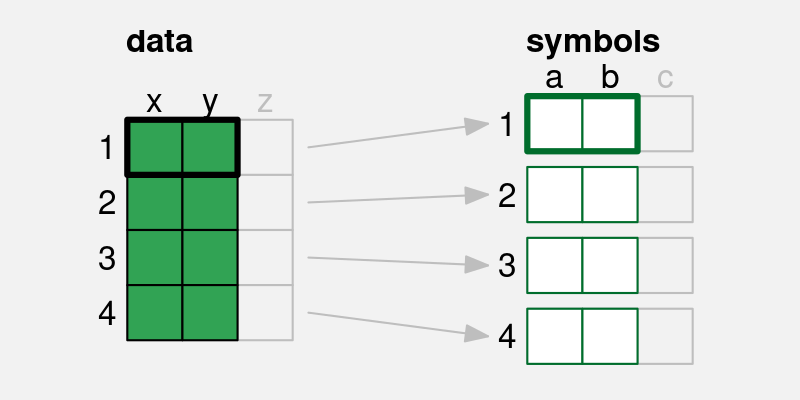
\includegraphics[scale=0.7]{Mappings/mapping-1-2-1-2.png}\end{minipage}%

\end{figure}%

}

\caption{\label{fig-two-visual-features}A simple data visualisation maps
\textbf{two} data values to \textbf{two} visual features to create a
data symbol. Each pair of data values (\texttt{a} and \texttt{b}) is
mapped to two visual features (\texttt{x} and \texttt{y}) of a
\textbf{single} data symbol.}

\end{figure}%

\section{Independent visual features}\label{independent-visual-features}

A bar plot involves encoding a qualitative variable as bar
\textbf{position} and a quantitative variable as bar \textbf{length}
(e.g., Figure~\ref{fig-bar}). We know that each visual feature is
effective on its own---we can decode from positions to qualitative
values and we can decode from lengths to quantitative values---but
another reason why the bar plot is effective overall is because the two
visual features act independently.\footnote{Refer to the literature that
  talks about separable and integral AND configural visual features.
  e.g., carswell and wickens (1990) looks at configural} Our perception
of the horizontal \textbf{length} of the bars is not affected by the
vertical \textbf{position} of the bars.\footnote{Technically, there is
  an interaction because lengths that are further apart from each other
  vertically are harder to compare (see
  Section~\ref{sec-distance-effect}). However, compared to visual
  features that strongly interact, length and position are reasonably
  independent.}

Figure~\ref{fig-bar-colour} demonstrates that we can also add
\textbf{colour} to the mix without creating any interactions between
visual features. The fact that the bottom two bars are blue and red does
not affect our ability to perceive that they have different lengths.

\begin{figure}

\centering{

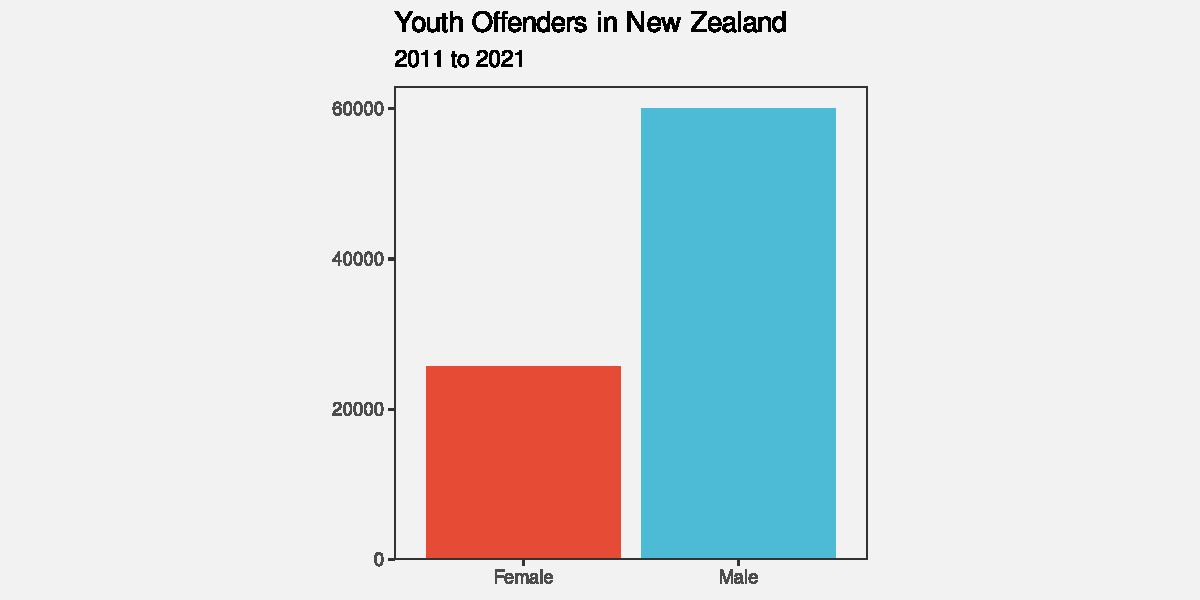
\includegraphics[width=1\linewidth,height=\textheight,keepaspectratio]{index_files/mediabag/combine_files/figure-pdf/fig-bar-colour-1.pdf}

}

\caption{\label{fig-bar-colour}A bar plot of the total number of
offenders for different ethnic groups. The data symbols in this plot
come from mapping ethnic group to the vertical positions and colours of
the bars and mapping the total number of offenders to the lengths of the
bars.}

\end{figure}%

\begin{quote}
One reason why a bar plot is effective is because data values are
encoded as visual features that can be decoded independently.
\end{quote}

\section{Scatter plots}\label{sec-integral}

Table~\ref{tbl-rwc-2023} shows data gathered on the performance of all
twenty teams at the 2023 Rugby World Cup. Most measures are positive,
for example, more \textbf{points} is better, but there are also a couple
of negative measures: more \textbf{tackles} may just mean that the team
was weak and was always being attacked; and more disciplinary
\textbf{cards} (either \textbf{y}ellow or \textbf{r}ed) is definitely a
bad sign.

\begin{longtable}[]{@{}
  >{\raggedright\arraybackslash}p{(\linewidth - 20\tabcolsep) * \real{0.1512}}
  >{\raggedright\arraybackslash}p{(\linewidth - 20\tabcolsep) * \real{0.0814}}
  >{\raggedleft\arraybackslash}p{(\linewidth - 20\tabcolsep) * \real{0.0814}}
  >{\raggedleft\arraybackslash}p{(\linewidth - 20\tabcolsep) * \real{0.0814}}
  >{\raggedleft\arraybackslash}p{(\linewidth - 20\tabcolsep) * \real{0.0814}}
  >{\raggedleft\arraybackslash}p{(\linewidth - 20\tabcolsep) * \real{0.0930}}
  >{\raggedleft\arraybackslash}p{(\linewidth - 20\tabcolsep) * \real{0.0814}}
  >{\raggedleft\arraybackslash}p{(\linewidth - 20\tabcolsep) * \real{0.1047}}
  >{\raggedleft\arraybackslash}p{(\linewidth - 20\tabcolsep) * \real{0.1047}}
  >{\raggedleft\arraybackslash}p{(\linewidth - 20\tabcolsep) * \real{0.0698}}
  >{\raggedleft\arraybackslash}p{(\linewidth - 20\tabcolsep) * \real{0.0698}}@{}}

\caption{\label{tbl-rwc-2023}Performance measures for all twenty teams
at the 2023 Rugby World Cup. Each measure is a per-game average because
some teams played more games than others.}

\tabularnewline

\toprule\noalign{}
\begin{minipage}[b]{\linewidth}\raggedright
country
\end{minipage} & \begin{minipage}[b]{\linewidth}\raggedright
sphere
\end{minipage} & \begin{minipage}[b]{\linewidth}\raggedleft
ycards
\end{minipage} & \begin{minipage}[b]{\linewidth}\raggedleft
rcards
\end{minipage} & \begin{minipage}[b]{\linewidth}\raggedleft
breaks
\end{minipage} & \begin{minipage}[b]{\linewidth}\raggedleft
tackles
\end{minipage} & \begin{minipage}[b]{\linewidth}\raggedleft
points
\end{minipage} & \begin{minipage}[b]{\linewidth}\raggedleft
converts
\end{minipage} & \begin{minipage}[b]{\linewidth}\raggedleft
offloads
\end{minipage} & \begin{minipage}[b]{\linewidth}\raggedleft
tries
\end{minipage} & \begin{minipage}[b]{\linewidth}\raggedleft
runs
\end{minipage} \\
\midrule\noalign{}
\endhead
\bottomrule\noalign{}
\endlastfoot
Namibia & South & 1.0 & 0.5 & 2.5 & 102.0 & 9.2 & 0.5 & 2.2 & 0.8 &
92.0 \\
Romania & North & 1.2 & 0.0 & 2.8 & 142.5 & 8.0 & 0.8 & 1.5 & 1.0 &
81.0 \\
Chile & South & 1.2 & 0.0 & 3.8 & 132.2 & 6.8 & 0.5 & 5.2 & 1.0 &
102.2 \\
Samoa & South & 1.2 & 0.2 & 3.8 & 109.5 & 23.0 & 2.0 & 9.2 & 2.8 &
102.5 \\
Australia & South & 0.5 & 0.0 & 5.2 & 108.2 & 22.5 & 1.8 & 7.8 & 2.8 &
110.8 \\
Georgia & North & 0.5 & 0.0 & 5.2 & 149.8 & 16.0 & 1.0 & 8.0 & 1.8 &
114.0 \\
Uruguay & South & 0.5 & 0.0 & 5.2 & 126.8 & 16.2 & 1.5 & 3.0 & 2.2 &
99.2 \\
South Africa & South & 0.4 & 0.0 & 5.4 & 139.1 & 29.7 & 2.7 & 5.4 & 3.9
& 95.1 \\
England & North & 0.0 & 0.1 & 5.6 & 124.9 & 31.6 & 2.3 & 3.9 & 3.0 &
100.3 \\
Fiji & South & 1.0 & 0.0 & 5.6 & 99.8 & 22.4 & 2.2 & 8.8 & 2.4 &
138.0 \\
Wales & North & 0.6 & 0.0 & 5.6 & 167.4 & 32.0 & 3.2 & 7.6 & 3.8 &
109.4 \\
Japan & North & 0.8 & 0.0 & 6.0 & 166.2 & 27.2 & 2.8 & 4.8 & 3.0 &
89.5 \\
Tonga & South & 0.5 & 0.2 & 6.0 & 141.2 & 24.0 & 2.0 & 8.2 & 3.2 &
107.5 \\
Argentina & South & 0.3 & 0.0 & 6.3 & 111.7 & 26.4 & 2.6 & 6.0 & 2.7 &
131.3 \\
Italy & North & 0.5 & 0.0 & 6.8 & 138.2 & 28.5 & 3.8 & 7.0 & 3.8 &
116.0 \\
Portugal & North & 0.5 & 0.2 & 7.8 & 148.0 & 16.0 & 1.5 & 9.2 & 2.0 &
118.2 \\
Ireland & North & 0.2 & 0.0 & 8.8 & 126.4 & 42.8 & 5.0 & 9.4 & 6.0 &
137.6 \\
France & North & 0.2 & 0.0 & 11.0 & 115.2 & 47.6 & 5.0 & 10.6 & 6.0 &
126.0 \\
Scotland & North & 0.2 & 0.0 & 11.2 & 123.0 & 36.5 & 4.8 & 13.8 & 5.2 &
151.2 \\
New Zealand & South & 0.7 & 0.3 & 12.6 & 123.4 & 48.0 & 5.0 & 8.3 & 7.0
& 139.3 \\

\end{longtable}

Figure~\ref{fig-scatter} shows a scatter plot of the number of ``clean
breaks'' per game versus the number of ``tries scored'' per game for
each team. A clean break means that a team has broken through the
opposition defence and a ``try scored'' means that the team has earned 5
points. A clean break implies an opportunity to score a try, but does
not guarantee that a try will be scored.

\begin{figure}

\centering{

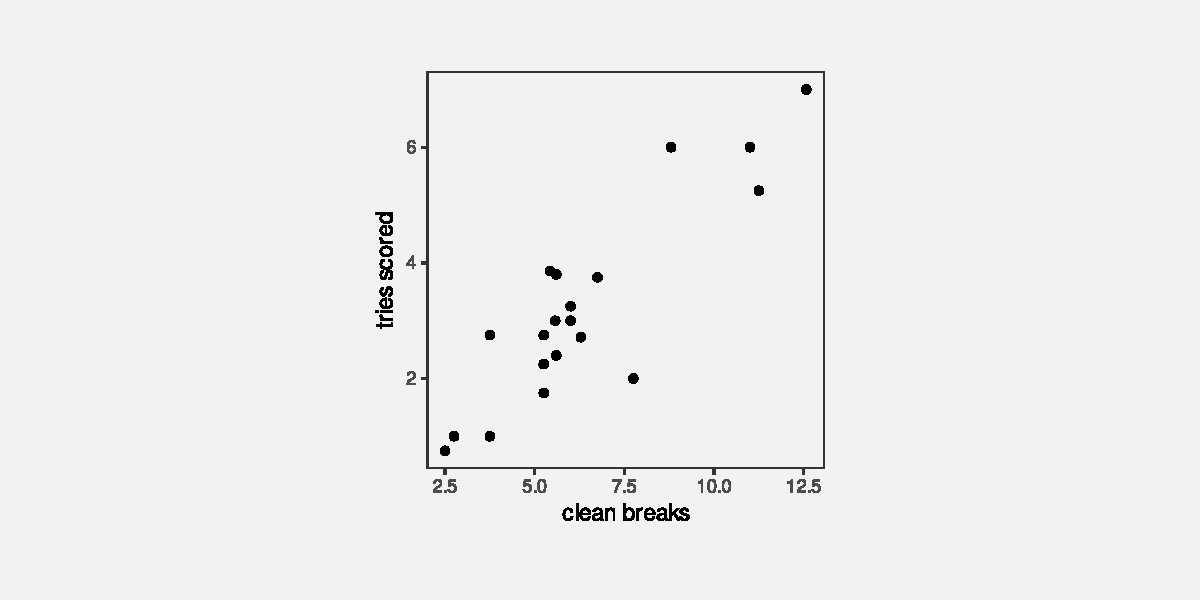
\includegraphics[width=1\linewidth,height=\textheight,keepaspectratio]{index_files/mediabag/combine_files/figure-pdf/fig-scatter-1.pdf}

}

\caption{\label{fig-scatter}A scatter plot of the number of times a team
breaks through the opposition defence and the number of tries that a
team scores (both are per-game averages) for teams at the 2023 Rugby
World Cup.}

\end{figure}%

The data symbol in a scatter plot is a data point, in this case a
circle. There are two mappings in the scatter plot in
Figure~\ref{fig-scatter}: the \textbf{quantitative} number of clean
breaks is encoded as the horizontal \textbf{position} of the data points
and the \textbf{quantitative} number of tries scored is encoded as the
vertical \textbf{position} of the data points.

We know from Chapter~\ref{sec-mapping-visual-features} that we should be
able to accurately decode the original data values from the positions of
the data points. For example, we can easily see that one team scored a
little over 7.5 clean breaks per game and we can see that two teams
scored about 6 tries per game.

However, there is something else going on in the scatter plot. The two
explicit encodings---horizontal and vertical
position---\textbf{interact} to create an additional visual
feature:\footnote{Need citations to literature that mention integral
  visual features. Admit a range rather than a dichotomy. Munzner has
  good examples?} \textbf{position in space}
(Figure~\ref{fig-interact}).\footnote{Relate this to mentions in
  literature of ``emergent features'', e.g., Pomerantz and Cragin
  (1994). Acknowledge that my use is a little loose because the use in
  the literature is really about separate data symbols combining to
  create emergent features (like clusters?). MacEachren 1995 uses
  emergent as ``configural'' (integral, but still also separable)
  ``Vision Science: Photons to Phenomenology'' Stephen Palmer, Figure
  2.1.5 caption ``The arrangement of several dots in a line give rise to
  emergent properties, such as length, orientation, and curvature, that
  are different from the properties of the dots that compose it.''

  NOTE that ``Emergent features and feature combination'' Pomerantz and
  Cragin (2014) (is this the same as Pomerantz and Cragin (1994) ???)
  explicitly differentiate between (fast) emergent features and
  ``normal'' (slow) feature integration that I am loosely using here.}
For example, we can perceive not only horizontal and vertical distances
between data points, but also euclidean distances between data points
(``as the crow flies'').

\begin{figure}

\centering{

\begin{figure}[H]

\begin{minipage}{0.50\linewidth}
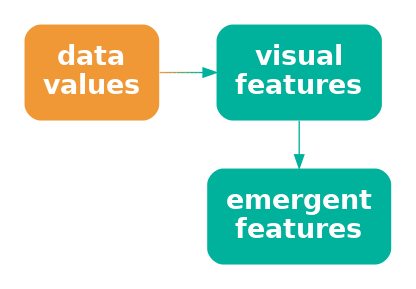
\includegraphics[scale=0.5]{Diagrams/data-vis-vis.png}\end{minipage}%

\end{figure}%

}

\caption{\label{fig-interact}If we encode data values as visual features
and the visual features interact, the result can be additional visual
features. It is possible for the additional visual feature to be
dominant relative to the original visual features or even to obscure the
original visual features.}

\end{figure}%

\begin{quote}
One reason why a scatter plot is effective at conveying relationships
between variables is because the mappings of data values to visual
features---horizontal position and vertical position---interact to
produce an additional visual feature: position in space.
\end{quote}

Furthermore, our visual system allows us to decode \textbf{visual
summaries} (see Section~\ref{sec-visual-summaries}) from
\textbf{position in space} (see
Figure~\ref{fig-visual-corr}).\footnote{Citations to literature on
  ensembles again, this time specifically to correlation in scatter
  plots. Talk about how, although there is some experimental support for
  reasonable accuracy of correlation from scatter plot (with some bias -
  specifically underestimation), there is not much experimental evidence
  for which is best for perceiving correlations Eg scatter plot vs
  parallel coords etc} For example, in Figure~\ref{fig-scatter} we can
easily see a positive \textbf{correlation} between the number of clean
breaks and the number of tries scored. We can also easily see
\textbf{clusters} of data points; the four data points in the top-right
corner of the plot appear separate from the other data points because
they share a similar position in space (see
Section~\ref{sec-visual-model-groups}).

\begin{figure}

\centering{

\begin{figure}[H]

\begin{minipage}{0.50\linewidth}
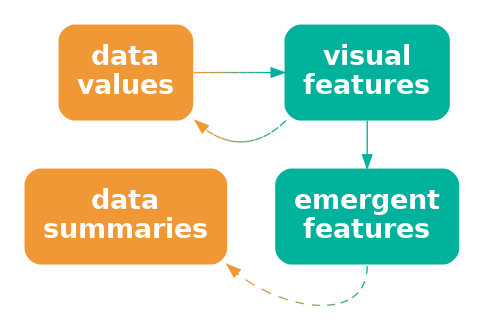
\includegraphics[scale=0.5]{Diagrams/data-vis-vis-stat.png}\end{minipage}%

\end{figure}%

}

\caption{\label{fig-visual-corr}If we encode data values as visual
features and the visual features interact, the result can be emergent
visual features. The original visual features allow us to decode raw
data values and the emergent features allow us to decode data
summaries.}

\end{figure}%

Although a scatter plot is similar to a bar plot because they both
involve two encodings---position and length for a bar plot and
horizontal position and vertical position for a scatter plot---there are
additional decodings possible from the data symbols in a scatterplot
because the additional visual feature of position in space emerges from
the combination of horizontal and vertical position.

\begin{quote}
One reason why a scatter plot is effective at conveying relationships
between variables is because we are able to decode visual summaries from
a collection of positions in space.
\end{quote}

\section{Case study: Mosaic plots}\label{sec-mosaic}

Table~\ref{tbl-offenders} shows a table of counts for offences committed
in New Zealand in 2021. For each offence, we know the sex of the
offender and what action was taken against the offender.

\begin{longtable}[]{@{}lrr@{}}

\caption{\label{tbl-offenders}Counts of offences committed in New
Zealand in 2021 by the sex of the offender and the action taken against
the offender.}

\tabularnewline

\toprule\noalign{}
& Female & Male \\
\midrule\noalign{}
\endhead
\bottomrule\noalign{}
\endlastfoot
Court Action & 13950 & 39526 \\
Non-Court Action & 8717 & 19663 \\
Not Proceeded With & 381 & 933 \\

\end{longtable}

Figure~\ref{fig-spine} shows a mosaic plot of the data in
Table~\ref{tbl-offenders}.\footnote{This two-dimensional mosaic plot
  could also be called a spine plot. Mosaic plot is the more general
  term that includes plots of more than two qualitative variables.} This
is an effective data visualisation for making several comparisons: the
overall proportion of male versus female offenders; within each sex, the
proportion of different actions against offenders; between sexes, the
distribution of different actions; and the overall proportions of
combinations of sex and action against offenders.

For example, we can see that there are more male offenders than female
offenders, court action is more common than non-court action for both
males and female offenders, court action is more common for male
offenders than for female offenders, and the most common offences
involve male offenders and result in court action.

\begin{figure}

\centering{

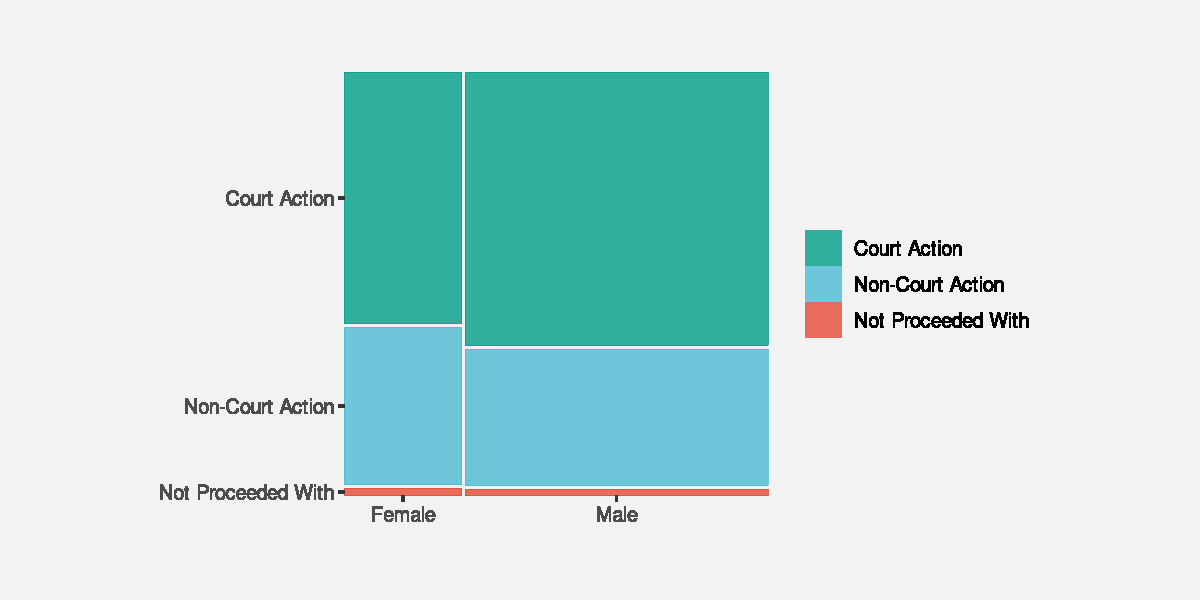
\includegraphics[width=1\linewidth,height=\textheight,keepaspectratio]{index_files/mediabag/combine_files/figure-pdf/fig-spine-1.pdf}

}

\caption{\label{fig-spine}A spine plot}

\end{figure}%

A mosaic plot is another example of a data visualisation that maps
\textbf{data summaries} to data symbols rather than raw data. The data
symbols are rectangles, the proportions of male versus female offenders
are encoded as the widths of the rectangles, and the proportions of
different actions taken, within males and females, are encoded as the
heights of the rectangles (see Table~\ref{tbl-offenders-summary}).

\begin{table}

\caption{\label{tbl-offenders-summary}The data summaries calculated from
Table~\ref{tbl-offenders} that are encoded as the widths and heights of
the rectangles in Figure~\ref{fig-spine}.}

\centering{

\subcaption{\label{tbl-offenders-summary-1}Widths}

\centering{

\begin{tabular}{lrr}
\toprule
 & Female & Male\\
\midrule
Court Action & 0.28 & 0.72\\
Non-Court Action & 0.28 & 0.72\\
Not Proceeded With & 0.28 & 0.72\\
\bottomrule
\end{tabular}

}

\subcaption{\label{tbl-offenders-summary-2}Heights}

\centering{

\begin{tabular}{lrr}
\toprule
 & Female & Male\\
\midrule
Court Action & 0.61 & 0.66\\
Non-Court Action & 0.38 & 0.33\\
Not Proceeded With & 0.02 & 0.02\\
\bottomrule
\end{tabular}

}

}

\end{table}%

\begin{quote}
One reason why a mosaic plot is effective is because it maps proportions
and conditional proportions, rather than raw counts, to the visual
features of rectangles.
\end{quote}

A mosaic plot is also an example of a data visualisation that maps to
visual features that \textbf{interact}. The explicit mappings involve
encoding proportions as the widths and heights of the rectangles and we
know from Section~\ref{sec-quant-features} that this will allow accurate
decoding from lengths to proportions.

\begin{quote}
One reason why a mosaic plot is effective is because it maps proportions
to lengths.
\end{quote}

However, the interaction of these mappings produces an \textbf{emergent
feature}, which is the \textbf{area} of the rectangles
(Figure~\ref{fig-interact}). Importantly, these areas correspond to
additional data summaries, in this case, the overall proportion of
offences in each combination of sex and action taken.

\begin{quote}
One reason why a mosaic plot is effective is because the mappings\\
to length and height interact to produce area, which represents overall
proportions.
\end{quote}

Mosaic plots also provide a simple visual check for independence between
factors. For example, in Figure~\ref{fig-spine} we can see that the
action taken is reasonably independent of the sex of the offender
because the heights of the rectangles are similar for both Male and
Female offenders (the conditional proportions are roughly the same).

One weakness of mosaic plots is that area is not the most accurate
visual feature (Section~\ref{sec-accuracy}), so we are not able to
decode overall proportions from the rectangle areas as accurately as we
are able to decode the proportions that are represented by the separate
widths and heights of the rectangles.

Another weakness is that the lengths and heights of the rectangles are
unaligned (Section~\ref{sec-unaligned}). This compromises the accuracy
of comparisons of widths between categories or the comparisons of
heights between categories. This weakness is greater if there are more
categories and/or larger differences between categories than we see in
Figure~\ref{fig-spine}. For example, Figure~\ref{fig-spine-weak} shows a
mosaic plot of the proportions of offenders in different age groups and,
within age groups, the proportions of actions against the offender at a
finer level of detail than in Figure~\ref{fig-spine}. If we attempt to
compare the proportion of offences that result in ``Formal Warnings'' in
younger age groups versus older age groups, we are hampered by the fact
that the pink rectangles do not have a common vertical baseline. As a
side note, we are also hampered in that case by the distance and
distractors between the rectangles (see
Section~\ref{sec-distance-effect}); the ordering of the variables and
the ordering of categories can have an impact on the effectiveness of a
mosaic plot just like ordering the bars of a bar plot.

\begin{figure}

\centering{

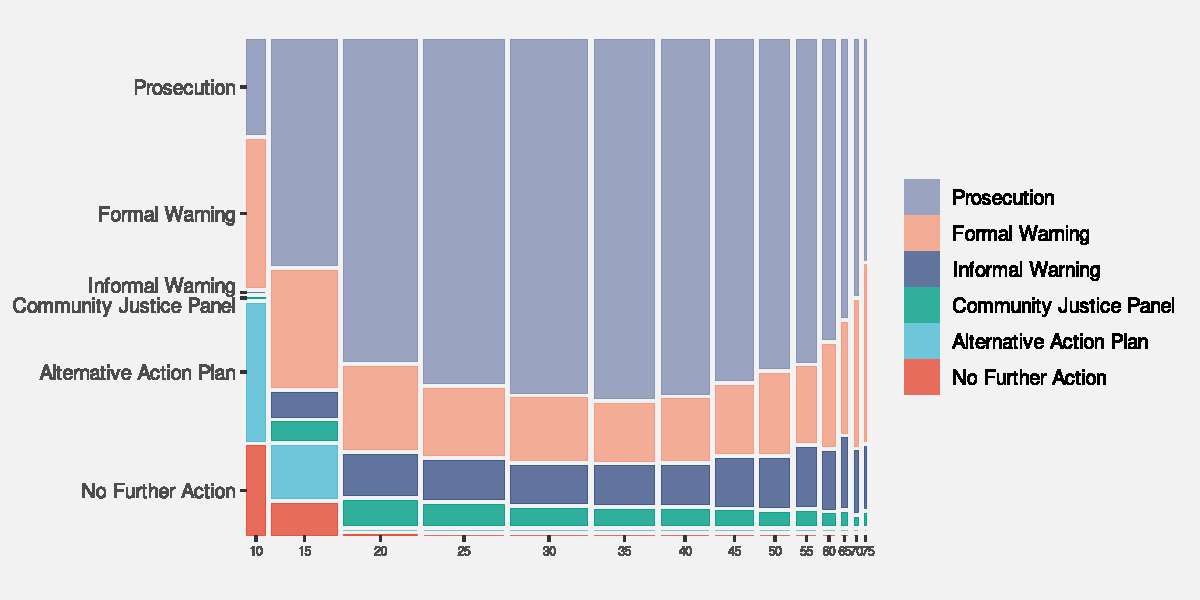
\includegraphics[width=1\linewidth,height=\textheight,keepaspectratio]{index_files/mediabag/combine_files/figure-pdf/fig-spine-weak-1.pdf}

}

\caption{\label{fig-spine-weak}A spine plot with problems}

\end{figure}%

These weaknesses are exacerbated for mosaic plots of more than two
variables. For example, the mosaic plot in Figure~\ref{fig-mosaic} shows
the proportions of youth versus adult offenders, then, within age
levels, the proportions of male versus female offenders, then, within
combinations of age levels and sex, the proportions of different actions
taken against the offender. Even though there are only very few levels
for each variable, our ability to compare heights and widths of
rectangles is impaired by inconsistent baselines, distance between
rectangles, and distractors.

\begin{figure}

\centering{

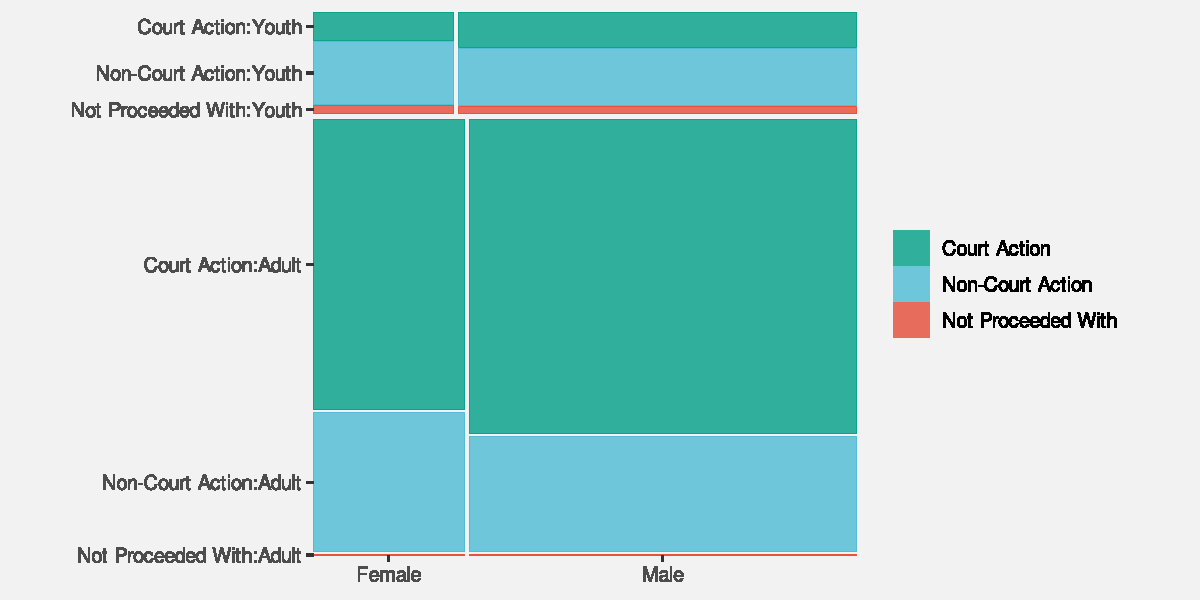
\includegraphics[width=1\linewidth,height=\textheight,keepaspectratio]{index_files/mediabag/combine_files/figure-pdf/fig-mosaic-1.pdf}

}

\caption{\label{fig-mosaic}A mosaic plot of three variables}

\end{figure}%

A final weakness with mosaic plots is that the \textbf{shape} of the
rectangles changes as well as the \textbf{area}. In
Section~\ref{sec-dissonance} we saw that changes in visual features
should only reflect changes in the data.

Figure~\ref{fig-area-shape} shows that we can create different
rectangles with the same area, but different shapes. There can be
rectangles within a mosaic plot with the same area, which represents the
same overall probability data value, but with different shapes. The
different shapes are a visual signal of differences in the data when in
reality no difference exists.

\begin{figure}

\centering{


\includegraphics[width=1\linewidth,height=\textheight,keepaspectratio]{index_files/mediabag/combine_files/figure-pdf/fig-area-shape-1.pdf}

}

\caption{\label{fig-area-shape}Three different shapes that all have the
same area.}

\end{figure}%

\section{Case study: Interaction
plots}\label{case-study-interaction-plots}

Figure~\ref{fig-interaction} shows an interaction plot of the number of
offenders in different ethnic groups, comparing 2011 to 2021. The raw
data are shown in Table~\ref{tbl-interaction}.

\begin{longtable}[]{@{}lrr@{}}

\caption{\label{tbl-interaction}The number of offenders in different
ethnic groups in 2011 and in 2021.}

\tabularnewline

\toprule\noalign{}
group & year & count \\
\midrule\noalign{}
\endhead
\bottomrule\noalign{}
\endlastfoot
Māori & 2011 & 5957 \\
Pasifika & 2011 & 1092 \\
European/Other & 2011 & 5775 \\
Unknown & 2011 & 194 \\
Māori & 2021 & 2869 \\
Pasifika & 2021 & 328 \\
European/Other & 2021 & 1833 \\
Unknown & 2021 & 1589 \\

\end{longtable}

The purpose of the interaction plot is to show the \emph{change} in the
number of offenders between 2011 and 2021 for each of the ethnic groups.
If the lines of the interaction plot were parallel we would conclude
that the same change has happened to all ethnic groups; the fact that
the lines are not parallel indicates that there have been different
changes in some ethnic groups compared to other ethnic
groups.\footnote{An interaction plot is typically used in a more
  experimental setting where the x-axis might be different treatments
  and the groups might be different patient groups and the y-axis might
  be a measure of response to treatment. The outcome is then whether the
  treatment has had the same effect for different patient groups (or
  not).}

\begin{figure}

\centering{

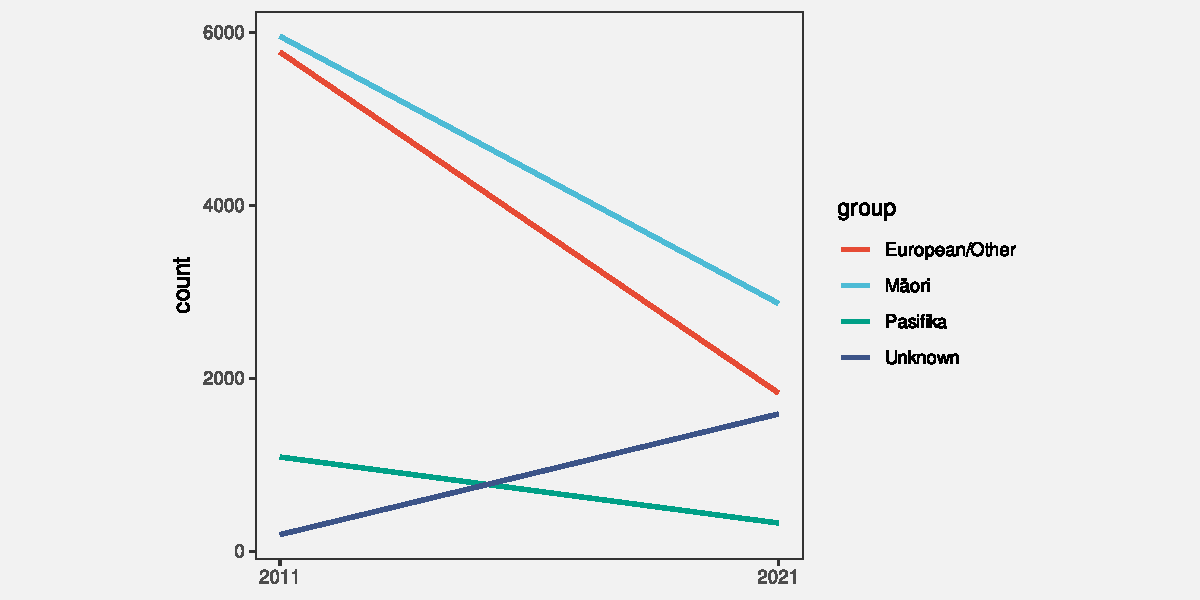
\includegraphics[width=1\linewidth,height=\textheight,keepaspectratio]{index_files/mediabag/combine_files/figure-pdf/fig-interaction-1.pdf}

}

\caption{\label{fig-interaction}An interaction plot showing the change
in the number of offenders in different ethnic groups between 2011 and
2021.}

\end{figure}%

The data symbols in Figure~\ref{fig-interaction} are straight line
segments. The year is encoded as the horizontal start and end
\textbf{position} of the lines and the number of offenders is encoded as
the vertical start and end \textbf{position} of the lines. The ethnic
group is encoded as the \textbf{colour} of the lines. These mappings are
effective for decoding the raw data values in
Table~\ref{tbl-interaction} from the end points and the colours of the
lines.

In addition, the explicit mappings generate an \textbf{emergent
feature}: the \textbf{angle} of the lines. Furthermore, the angle of the
lines allow us to decode a \textbf{data summary}: the \emph{change} in
the number of offenders between 2011 and 2021 (see
Figure~\ref{fig-visual-corr}).

\begin{quote}
An interaction plot is effective because it allows us to decode changes
in the data values from the angles of the lines.
\end{quote}

It is more difficult to perceive the \emph{change} in the number of
offenders for each ethnic group in a bar plot like the one shown in
Figure~\ref{fig-interaction-bar}. Partly this is because we have to
decode the lengths of two bars for each ethnic group rather than the
slope of a single line.\footnote{Pinker 1990, p.~111 talks about the
  difficulty of extracting different sorts of information from different
  data symbols (bars vs lines).}

\begin{figure}

\centering{

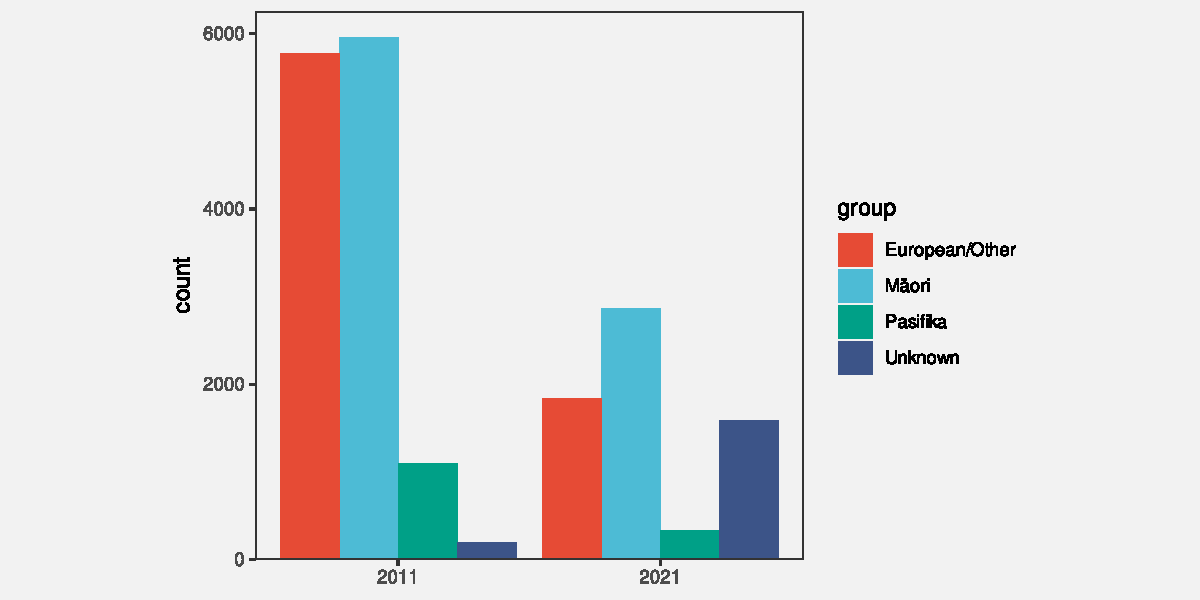
\includegraphics[width=1\linewidth,height=\textheight,keepaspectratio]{index_files/mediabag/combine_files/figure-pdf/fig-interaction-bar-1.pdf}

}

\caption{\label{fig-interaction-bar}A bar plot showing the number of
offenders in different ethnic groups in 2011 and in 2021.}

\end{figure}%

\section{Dangers of combining
mappings}\label{dangers-of-combining-mappings}

Figure~\ref{fig-nz-doctor-bar} shows a plot of changes in health
spending by successive New Zealand governments.\footnote{Figure~\ref{fig-nz-doctor-bar}
  is based on Figure 2 from Huskinson (2024).} In this data
visualisation, the average change in health spending over a government's
entire term is encoded as the \textbf{height} of a bar, with the
duration of that government's term encoded as the \textbf{width} of the
bar. Because height and width are visual features that interact, the
result is an \textbf{area} for each government's term. However, that
area has no sensible interpretation; what does a percent multiplied by a
number of years mean? The areas of the bars do not correspond to any
property of the data values.

\begin{figure}

\centering{

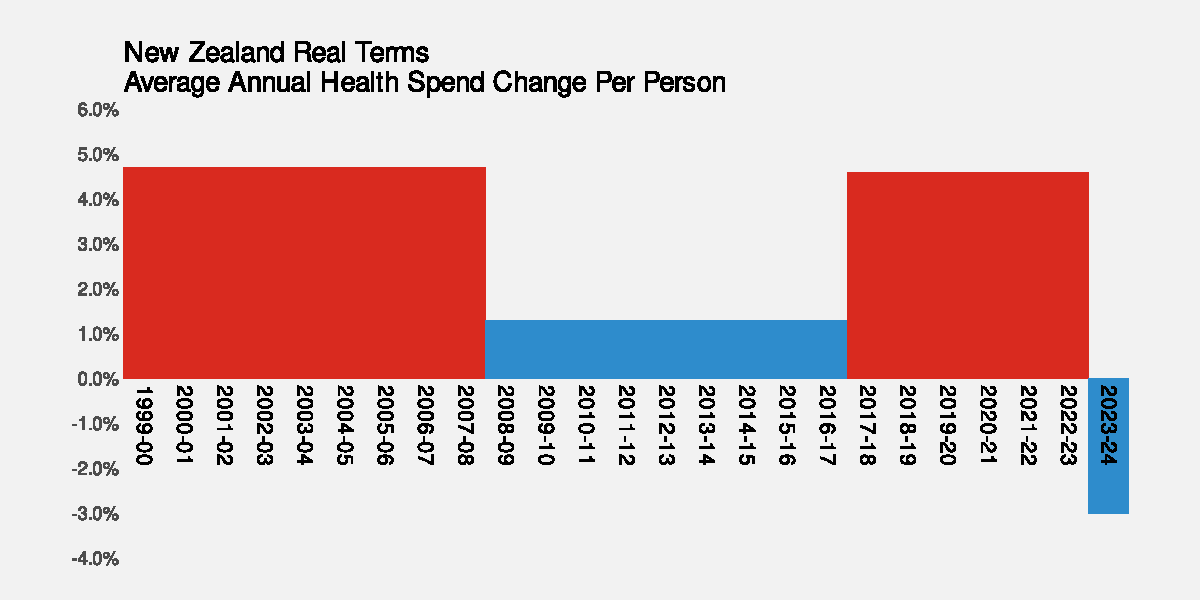
\includegraphics[width=1\linewidth,height=\textheight,keepaspectratio]{index_files/mediabag/combine_files/figure-pdf/fig-nz-doctor-bar-1.pdf}

}

\caption{\label{fig-nz-doctor-bar}A plot showing the differences in
health spending for successive New Zealand governments using filled
bars.}

\end{figure}%

The interaction of visual features can be a boon when the interaction
produces an emergent feature that can be decoded to properties of the
data (as in a scatter plot, or mosaic plot, or interaction plot).\\
However, it is possible to create a poor data visualisation if we
produce an emergent feature that has no correspondence with data values
(Figure~\ref{fig-data-vis-vis-lie}).\footnote{This is the
  ``compatibility principle'' ? of Carswell and Wickens ?}

\begin{figure}

\centering{

\begin{figure}[H]

\begin{minipage}{0.50\linewidth}
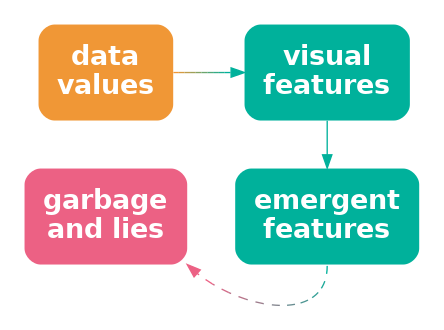
\includegraphics[scale=0.5]{Diagrams/data-vis-vis-lie.png}\end{minipage}%

\end{figure}%

}

\caption{\label{fig-data-vis-vis-lie}If we encode data values as visual
features and the visual features interact, the result can be emergent
visual features. However, this is only appropriate if the emergent
features correspond to some property of the data. Otherwise, the
decoding may lead to unhelpful and misleading interpretations.}

\end{figure}%

Figure~\ref{fig-nz-doctor-line} shows a different representation of the
data. In this case, the average change in health spending is encoded as
the (vertical) \textbf{position} of a line and the duration is encoded
as the \textbf{length} of the line. These visual features do not
interact, so we no longer have a misleading emergent visual feature.

\begin{figure}

\centering{

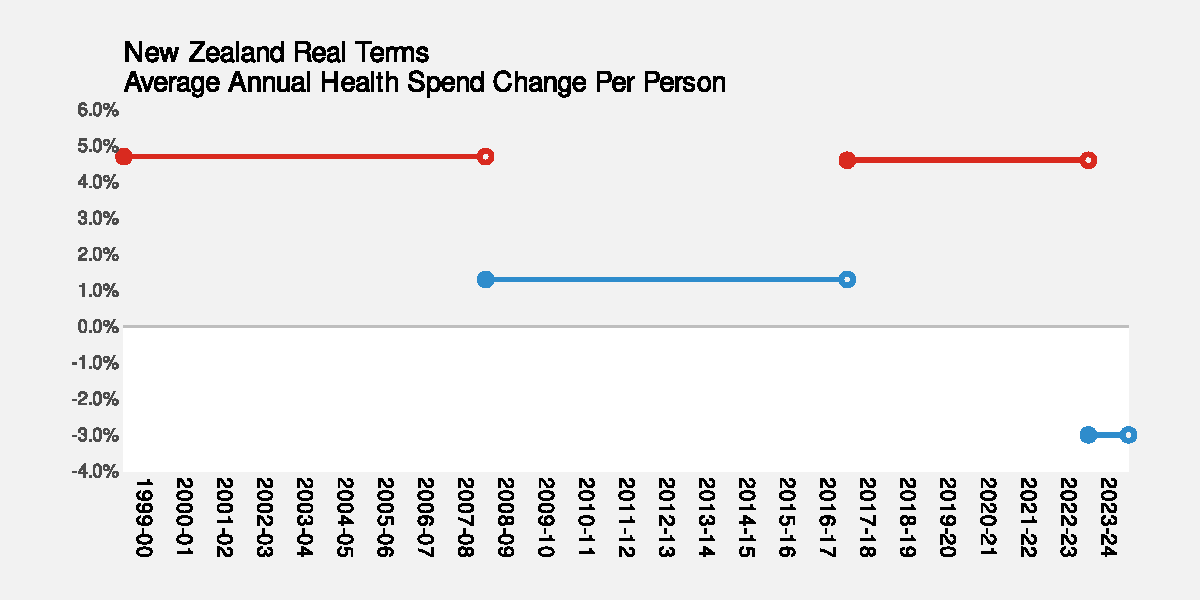
\includegraphics[width=1\linewidth,height=\textheight,keepaspectratio]{index_files/mediabag/combine_files/figure-pdf/fig-nz-doctor-line-1.pdf}

}

\caption{\label{fig-nz-doctor-line}A plot showing the differences in
health spending for successive New Zealand governments using horizontal
lines.}

\end{figure}%

\textbf{There is also the problem of separable when integral would be
appropriate (reduce to separate effects inappropriately?)} Is there an
example?

\textbf{Must} say that chroma and luminance and hue are all integral. Is
this an example of integrating ineffectively?

\section{Redundant mappings}\label{sec-redundant}

In Section~\ref{sec-mosaic}, we focused on the encoding of quantitative
values (proportions) as the widths and heights of the rectangular data
symbols in a mosaic plot, for example, Figure~\ref{fig-spine}. There are
also qualitative values encoded in a mosaic plot: the different
categories, like Male and Female.

The main encoding of the categories in a mosaic plot is as the
\textbf{position} of the rectangles. For example, in
Figure~\ref{fig-spine}, the rectangles for Female are to the left and
the rectangles for Male are to the right and the rectangles for
different court actions are stacked vertically, with Not Proceeded With
at the bottom, Non-Court Action in the middle, and Court Action at the
top.

In addition, different court actions are encoded as different
\textbf{colours}. This additional encoding is \textbf{redundant} in the
sense that we can already decode the court action from the vertical
position of the bars. However, having the additional encoding means that
we have two ways to decode the court action: from the vertical position
and from the colour. This becomes much more useful when there are more
categories (Figure~\ref{fig-spine-weak}) or more variables
(Figure~\ref{fig-mosaic}).\footnote{``Clusters Beat Trend!? Testing
  Feature Hierarchy in Statistical Graphics'' VanderPlas and Hofmann
  (2017) says redundancy helps

  ``Beyond Memorability: Visualization Recognition and Recall'' Borkin
  et al (2015) also says redundancy helps

  ``The Science of Visual Data Communication: What Works'' Franconeri et
  al (2021) says it doesn't (though only with expert opinion like Tukey
  to back it up. Exception is to allow for colour-blind viewers.}

\begin{figure}

\centering{

\begin{figure}[H]

\begin{minipage}{0.50\linewidth}
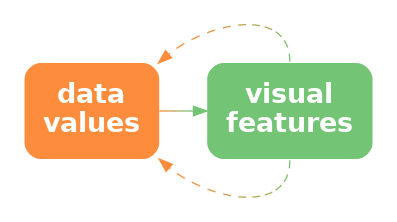
\includegraphics[scale=0.5]{Diagrams/data-vis-redundant.png}\end{minipage}%
%
\begin{minipage}{0.50\linewidth}
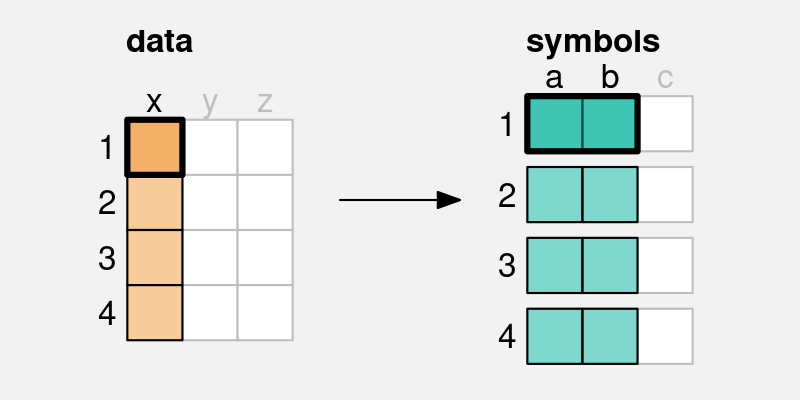
\includegraphics[scale=0.7]{Mappings/mapping-1-1-1-2.png}\end{minipage}%

\end{figure}%

}

\caption{\label{fig-data-vis-redundant}A redundant encoding maps a
single data value to multiple visual features. Each data value
(\texttt{a}) is mapped to not just one visual feature (\texttt{x}), but
also a second visual feature (\texttt{y}), of a single data symbol. If
we encode data values using multiple visual features, then multiple
decodings are possible.}

\end{figure}%

One useful application of redundant encoding is to accommodate viewers
with CVD (Section~\ref{sec-CVD}). Having a secondary decoding alongside
colour allows for the fact that the colour decoding may fail for some
viewers.

\section{Summary}\label{summary-8}

The mappings involved in a bar plot---quantitative data values encoded
as lengths and qualitative values encoded as position---are effective
because we are able to perceive some combinations of visual features,
such as length, position, and colour \textbf{independently}.

A scatter plot is effective for perceiving relationships between
variables because the mappings of quantitative data values to both
horizontal and vertical positions \textbf{interact} to produce
\textbf{position in space} and our visual system is capable of producing
useful \textbf{visual summaries} of position in space, such as
correlation.

The effectiveness of a mosaic plot also depends upon the
\textbf{interaction} of visual features: marginal and conditional
proportions are mapped to widths and heights, which produce
\textbf{area} to represent overall proportions.

Care must be taken to avoid generating emergent features that do not
represent any meaningful property of the data.

\begin{center}\rule{0.5\linewidth}{0.5pt}\end{center}

\theendnotes

\bookmarksetup{startatroot}

\chapter{Visual Shapes}\label{sec-visual-shapes}

All of the data visualisations that we have considered so far have
mapped a \textbf{single data value} from one or more variables to a
\textbf{single data symbol} (Figure~\ref{fig-multivariate-symbol-a}).
For example, a bar plot like Figure~\ref{fig-bar} maps one category and
one count to one bar. A scatter plot like Figure~\ref{fig-scatter} maps
one data value from a quantitative variable and one data value from
another quantitative variable to one data point.

In this section, we consider data visualisations that map
\textbf{multiple data values} from one or more variables to a
\textbf{single data symbol} (Figure~\ref{fig-multivariate-symbol-b}). In
this section, we begin to consider more complex data symbols.

\begin{figure}

\centering{

\begin{figure}[H]

\begin{minipage}{0.50\linewidth}

\centering{

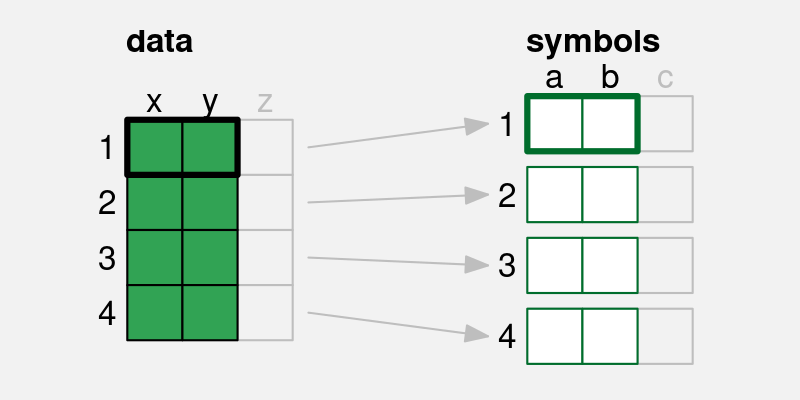
\includegraphics[scale=0.7]{Mappings/mapping-1-2-1-2.png}

}

\subcaption{\label{fig-multivariate-symbol-a}}

\end{minipage}%
%
\begin{minipage}{0.50\linewidth}

\centering{

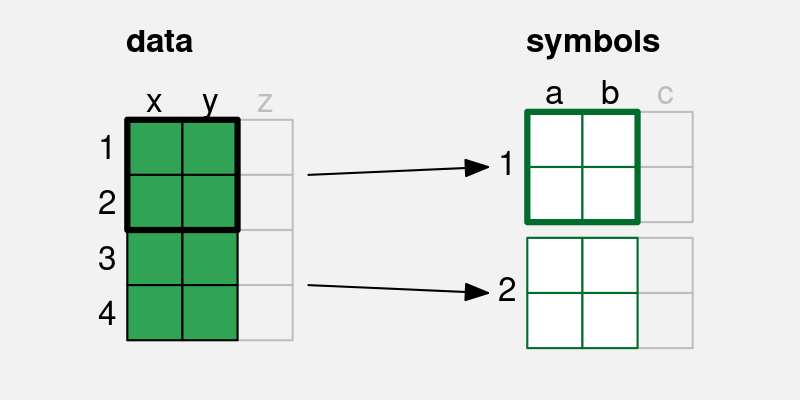
\includegraphics[scale=0.7]{Mappings/mapping-2-2-1-2.png}

}

\subcaption{\label{fig-multivariate-symbol-b}}

\end{minipage}%

\end{figure}%

}

\caption{\label{fig-multivariate-symbol}(a) A simple data symbol, like a
bar in a bar plot or a data point in a scatter plot involves mapping
\textbf{one} data value from each of two variables to two visual
features of \textbf{one} data symbol; a single pair of data values
produces a single data symbol (this is a reproduction of the diagram in
Figure~\ref{fig-two-visual-features}). (b) A more complex data symbol is
produced if we map \textbf{multiple} data values from each of two
variables to two visual features of a \textbf{single} data symbol.
Multiple data values from \texttt{a} and \texttt{b} are mapped to the
visual features, \texttt{x} and \texttt{y}, of a single data symbol.
Multiple pairs of values produce a single data symbol.}

\end{figure}%

\section{Line plots}\label{sec-line-plots}

Figure~\ref{fig-line} shows a line plot of the number of offenders per
year in different ethnic groups from 2011 to 2021 (see
Table~\ref{tbl-crime-group-year}). This data visualisation is very
effective for perceiving changes over time in the number of offenders
within each group as well as comparing the changes over time between
groups.

\begin{figure}

\centering{

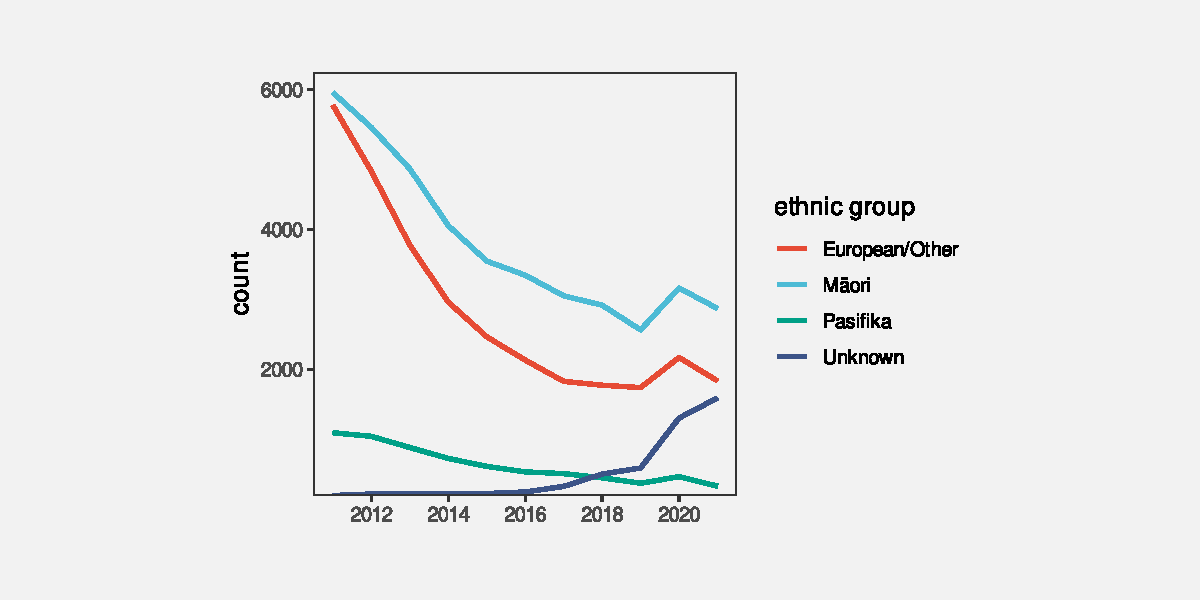
\includegraphics[width=1\linewidth,height=\textheight,keepaspectratio]{index_files/mediabag/visual-shapes_files/figure-pdf/fig-line-1.pdf}

}

\caption{\label{fig-line}A line plot of the number of offenders per year
in different ethnic groups from 2011 to 2021.}

\end{figure}%

There are some familiar mappings in this data visualisation: year is
mapped to horizontal \textbf{position}, the number of offenders is
mapped to vertical \textbf{position}, and the ethnic group is mapped to
\textbf{colour}. However, the \textbf{data symbols} in this data
visualisation, the coloured lines, are different from any previous
examples that we have seen. Although there are 44 rows of data, there
are only 4 data symbols. Multiple rows of data are used to create each
data symbol. Each coloured line in Figure~\ref{fig-line} represents 11
pairs of year and count values.

This contrasts with visualisations like bar plots that use simpler data
symbols. For example, the bar plot of the same data in
Figure~\ref{fig-side-bar-year} has 44 bars.

Figure~\ref{fig-line} is effective at conveying changes over time
because the coloured lines create \textbf{visual shapes}
(Figure~\ref{fig-data-vis-shape}) and those visual shapes convey
information about collections of data values. For example, we can
perceive slopes and curves and peaks and valleys in each of the coloured
lines.\footnote{``VISUAL PATTERN RECOGNITION'' Few (2006) Makes this
  same point {[}p 10{]} Demonstration of difference between density plot
  (mostly see a shape) and histogram (mostly see bar heights).}

\begin{figure}

\centering{

\begin{figure}[H]

\begin{minipage}{0.50\linewidth}
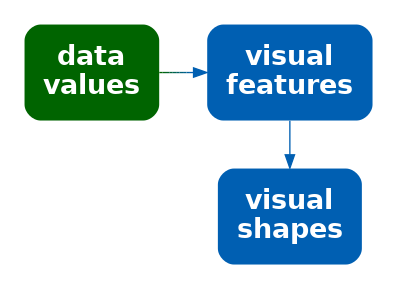
\includegraphics[scale=0.5]{Diagrams/data-vis-shape.png}\end{minipage}%

\end{figure}%

}

\caption{\label{fig-data-vis-shape}If we map multiple data values to
multiple visual features of a single data symbol, like in a line plot,
we create a smaller number of more complex data symbols, \textbf{visual
shapes}, that contain a larger amount of information.}

\end{figure}%

In terms of the simple visual processing model from
Section~\ref{sec-visual-processing}, these more complicated shapes can
convey more sophisticated information, at the expense of more cognitive
effort, and with a limit on how many shapes we can process
simultaneously (see Figure~\ref{fig-visual-model}). In other words, the
more complex data symbols allow us to decode \textbf{data summaries}
(Figure~\ref{fig-data-vis-shape-decode}). For example, in
Figure~\ref{fig-line} we are able to perceive overall trends in the
number of offenders, periods of more rapid change versus periods of
slower change, and local maxima and minima.\footnote{``Understanding
  Charts and Graphs'' Kosslyn (1989) {[}somewhere after p 205{]} Lines
  are objects ``For example, if one wants a reader to see an
  interaction, a line graph is better than a bar graph: not only is a
  line a single perceptual unit, and hence there will be less to hold in
  short-term memory, but we are good at detecting slope
  differences-which convey the relevant information (see Pinker,
  1988).''}

\begin{figure}

\centering{

\begin{figure}[H]

\begin{minipage}{0.50\linewidth}
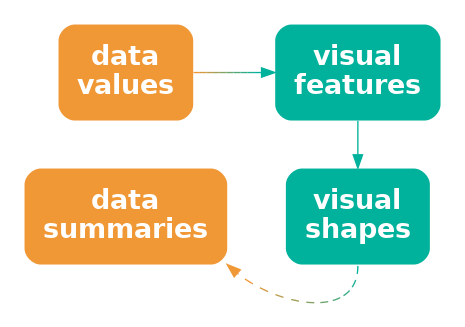
\includegraphics[scale=0.5]{Diagrams/data-vis-shape-decode.png}\end{minipage}%

\end{figure}%

}

\caption{\label{fig-data-vis-shape-decode}If we map data values to a
\textbf{visual shape} that contains a large amount of information, then
we may be able to decode more sophisticated \textbf{data summaries}.}

\end{figure}%

In terms of Chapter~\ref{sec-congruence}, the use of lines for data
symbols is also \textbf{congruent} with trends in the data; we naturally
associate slopes with increases and decreases in data values.\footnote{According
  to Zacks and Tversky 1999 people use ``trend words''
  (increasing/decreasing) versus ``discrete words'' (higher/lower than)
  AND are faster to judge absolute values from bars but angle from line
  graphs.}

\begin{quote}
One reason why line plots are effective is because they encode multiple
data values into a complex data symbol that creates a visual shape, from
which we are able to decode data summaries.
\end{quote}

On the other hand, the more complex data symbols in a line plot, that
contain multiple data values, are less effective at conveying the
\emph{individual} raw data values. The coloured lines in
Figure~\ref{fig-line} are not simple shapes from which it is easy to
perceive basic \textbf{visual features}. This means that, although we
may be able to decode data summaries, it is not easy to decode the raw
data values (Figure~\ref{fig-data-vis-shape-decode}). For example,
compare the ease with which we can determine the number of
European/Other offenders in 2013 from Figure~\ref{fig-line} versus
Figure~\ref{fig-side-bar-year}.

This deficiency is significant because the main mappings in a line plot
are from \textbf{quantitative} data values to (horizontal and vertical)
\textbf{position}. We know from
Chapter~\ref{sec-mapping-visual-features} that these should be very
effective mappings that allow us to accurately decode the raw data
values. However, in a line plot, we are not mapping a single data value
to a basic visual feature of a single, simple shape. Instead, a single
data value is being mapped, along with many other values, to a basic
visual feature of a complicated shape. In effect, the individual data
values lose their individual identity.\footnote{citation for surjective,
  injective, bijective

  Adam has a nice example in his thesis Figure 4.5, a simpler version of
  which is a line or bar plot that contains a ``total'' line or bar -
  the visual objects do not map neatly, and disjointly to subsets of the
  data - there is overlap. This makes mapping back to the data harder or
  at least more ambiguous ?}

\begin{quote}
One reason why a line plot is \emph{less} effective for decoding raw
data values is because each raw data value is not mapped to its own data
symbol.
\end{quote}

The creation of complex data symbols from multiple data values bears
some similarity to the creation of emergent features by combining visual
features (Section~\ref{sec-integral}). In both cases, we have
\emph{explicit} encodings from data values to basic visual features, but
we also produce an \emph{implicit} additional visual effect. The
difference here is that with complex data symbols, we are collapsing
multiple data values into a data symbol, so we run a higher risk of
losing the ability to perceive individual data values.\footnote{Also
  link to ``configural displays'' (David Peebles (2008)) and ``display
  proximity'' (Barnett \& Wickens, 1988; Carswell \& Wickens, 1987;
  Wickens \& Andre, 1990) ``According to the proximity compatibility
  principle (Wickens \& Carswell, 1995), representations with high
  display proximity facilitate high mental proximity tasks requiring the
  integration of information from multiple sources. The relationship
  between display and mental proximity has been revealed in several
  studies (e.g., Barnett \& Wickens, 1988; Bennett \& Flach, 1992;
  Bennett, Toms, \& Woods, 1993; Carswell \& Wickens, 1987; Wickens \&
  Andre, 1990; Wickens \& Carswell, 1995) and it is argued that the
  advantage comes when emergent features (Pomerantz \& Pristach, 1989)
  of the representation indicate additional information about the
  domain.'' He also mentions line plots as being in between separable
  bar plots and configural radar plots.}

There is also a similarity between complex data symbols and visual
summaries (Section~\ref{sec-visual-summaries}). In both cases, we gain
the ability to decode data summaries from collections of data values.
Again, the difference is that with visual summaries, we are summarising
many simple data symbols that each represent individual data values,
whereas with a complex data symbol we decode the data summary from a
single data symbol that obscures the individual data values.

\section{Case study: Scatter plots with
lines}\label{case-study-scatter-plots-with-lines}

Figure~\ref{fig-line-points} shows a data visualisation of the number of
offenders per year in different ethnic groups
(Table~\ref{tbl-crime-group-year}). This is very similar to
Figure~\ref{fig-line}, but we have added a data point at every
horizontal and vertical \textbf{position}.

Like Figure~\ref{fig-line}, we can decode overall trends from the line
data symbols, but we can also decode individual data values more easily
because now every individual data value is also mapped to its own data
symbol.

\begin{figure}

\centering{

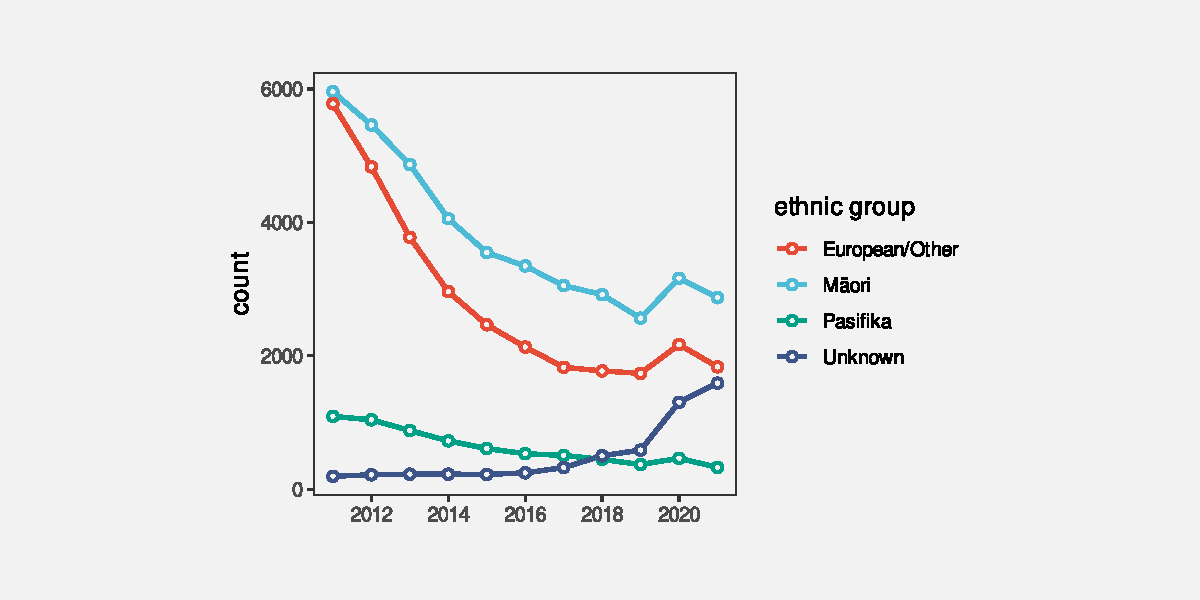
\includegraphics[width=1\linewidth,height=\textheight,keepaspectratio]{index_files/mediabag/visual-shapes_files/figure-pdf/fig-line-points-1.pdf}

}

\caption{\label{fig-line-points}A plot of the number of offenders per
year in different ethnic groups from 2011 to 2021 with both lines and
points.}

\end{figure}%

\section{Case study: Density plots}\label{sec-density}

Figure~\ref{fig-density} shows a density plot of the number of points
scored by Tier One nations at the Rugby World Cups
(Table~\ref{tbl-rwc-all}). As with a histogram (Figure~\ref{fig-hist}),
this data visualisation is effective for conveying the distribution of
data values. For example, we can perceive that there is evidence of a
single mode and right skew.

\begin{figure}

\centering{

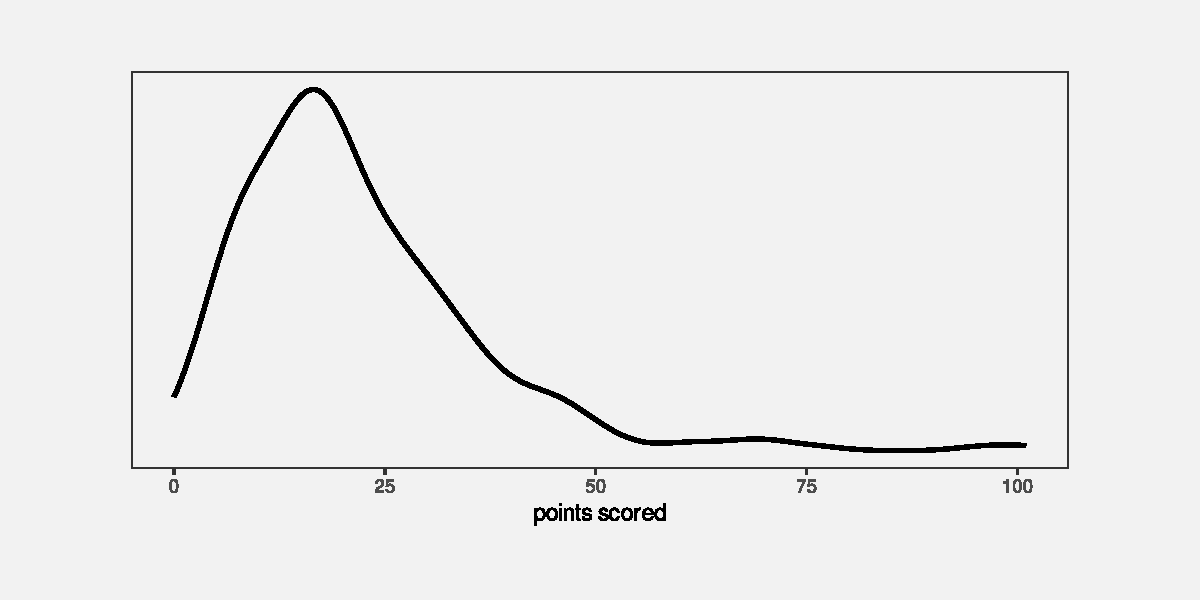
\includegraphics[width=1\linewidth,height=\textheight,keepaspectratio]{index_files/mediabag/visual-shapes_files/figure-pdf/fig-density-1.pdf}

}

\caption{\label{fig-density}A density plot of the points scored per game
by Tier One nations at Rugby World Cups.}

\end{figure}%

Also like a histogram, a density plot actually maps \textbf{data
summaries}, density estimates rather than raw data values, to visual
features (see Table~\ref{tbl-density-stats}). In the case of a
histogram, the data summary values are counts within bins (see
Table~\ref{tbl-hist-stats}) and each data summary produces a separate
bar. However, a density plot encodes all of the data summary values to a
single data symbol, a line, to create a \textbf{visual shape}. The
density estimates are mapped to the horizontal and vertical
\textbf{positions} of a single line data symbol. The visual shape allows
us to perceive summaries of the density estimates. For example, whether
there is a single maximum density and how the density changes to either
side of that peak.

\begin{longtable}[]{@{}rr@{}}

\caption{\label{tbl-density-stats}A table of density estimates at a
sample of values over the range of the number of points scored by Tier
One nations in Rugby World Cup matches. These data summaries are the
values that are mapped to visual features to produce the density plot in
Figure~\ref{fig-density}. There are 512 rows of values, but only the
first 6 are shown here.}

\tabularnewline

\toprule\noalign{}
scored & density \\
\midrule\noalign{}
\endhead
\bottomrule\noalign{}
\endlastfoot
0.00 & 0.0055 \\
0.20 & 0.0059 \\
0.40 & 0.0063 \\
0.59 & 0.0067 \\
0.79 & 0.0071 \\
0.99 & 0.0075 \\

\end{longtable}

Figure~\ref{fig-data-stat-vis-shape-stat} shows the path from raw data
values to data summaries (density estimates), which are encoded as the
visual features (horizontal and vertical position) of a visual shape (a
line) in a density plot and the summary information that we can decode
from the visual shape. We cannot decode the raw data values from a
density plot, nor can we very easily decode the data summaries (the
density estimates). The only real purpose of the data symbol in a
density plot is to allow us to decode \textbf{summaries} of the data
summaries, which are visual features of the density estimates (like the
number of peaks and where the peaks occur).

\begin{figure}

\centering{

\begin{figure}[H]

\begin{minipage}{0.50\linewidth}
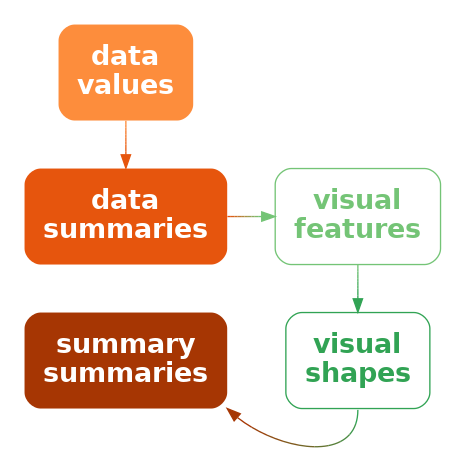
\includegraphics[scale=0.5]{Diagrams/data-stat-vis-shape-stat.png}\end{minipage}%

\end{figure}%

}

\caption{\label{fig-data-stat-vis-shape-stat}A density plot maps data
summaries to visual features to create a visual shape from which we can
decode \textbf{summaries} of the data summaries.}

\end{figure}%

\begin{quote}
A density plot is effective because it conveys high-level features of
density estimates of the raw data.
\end{quote}

Another commonality between density plots and histograms is that we get
to choose how the data summaries are calculated from the raw data
values. In the case of a density plot, we must choose a ``kernel'' and a
``bandwidth'', both of which affect the smoothness of the density
estimates. This means that we may need to explore more than one kernel
and bandwidth (see Section~\ref{sec-summary-caveats}).

A final point about density plots, especially in comparison to
histograms is that it is more effective to present multiple density
curves, rather than multiple histograms. This is demonstrated in
Figure~\ref{fig-multiple-density} and Figure~\ref{fig-multiple-hist}.
Multiple histograms overlap each other, which makes it difficult to
perceive the separate histograms and this is not satisfactorily solved
by adding semitransparency. By comparison, multiple density curves
create very little overlap, and even though the orange curve passes
``under'' the blue curve, we effortlessly perceive the orange curve as a
single, coherent shape (see Section~\ref{sec-visual-model-groups}).

\begin{figure}

\centering{

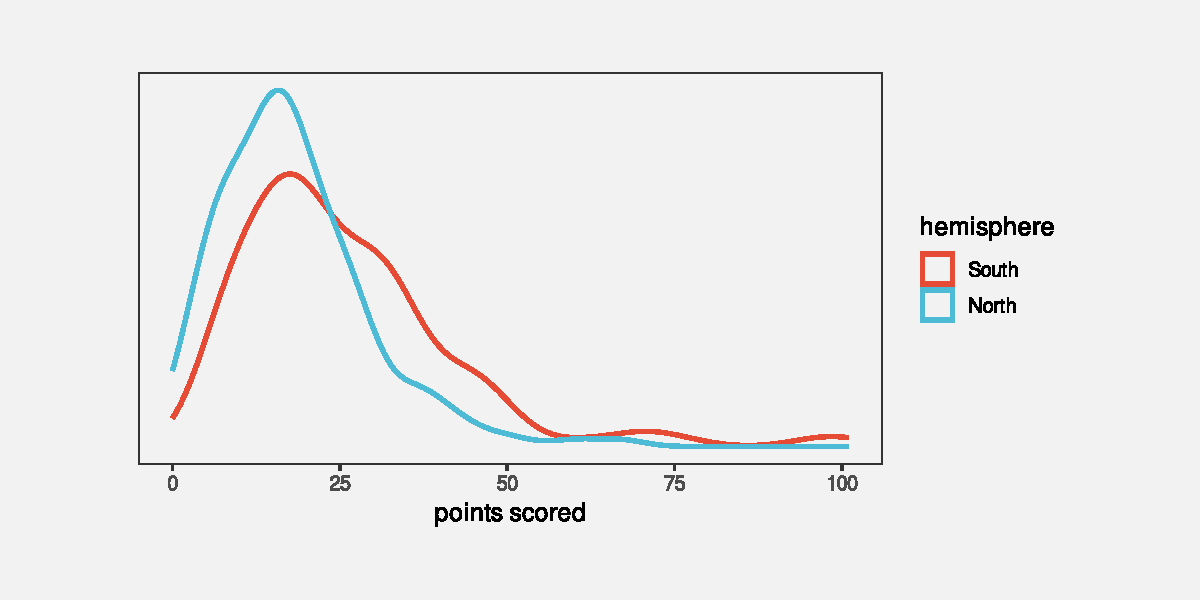
\includegraphics[width=1\linewidth,height=\textheight,keepaspectratio]{index_files/mediabag/visual-shapes_files/figure-pdf/fig-multiple-density-1.pdf}

}

\caption{\label{fig-multiple-density}Density plots of the points scored
per game by Tier One nations at Rugby World Cups, broken down by
hemisphere.}

\end{figure}%

\begin{figure}

\centering{

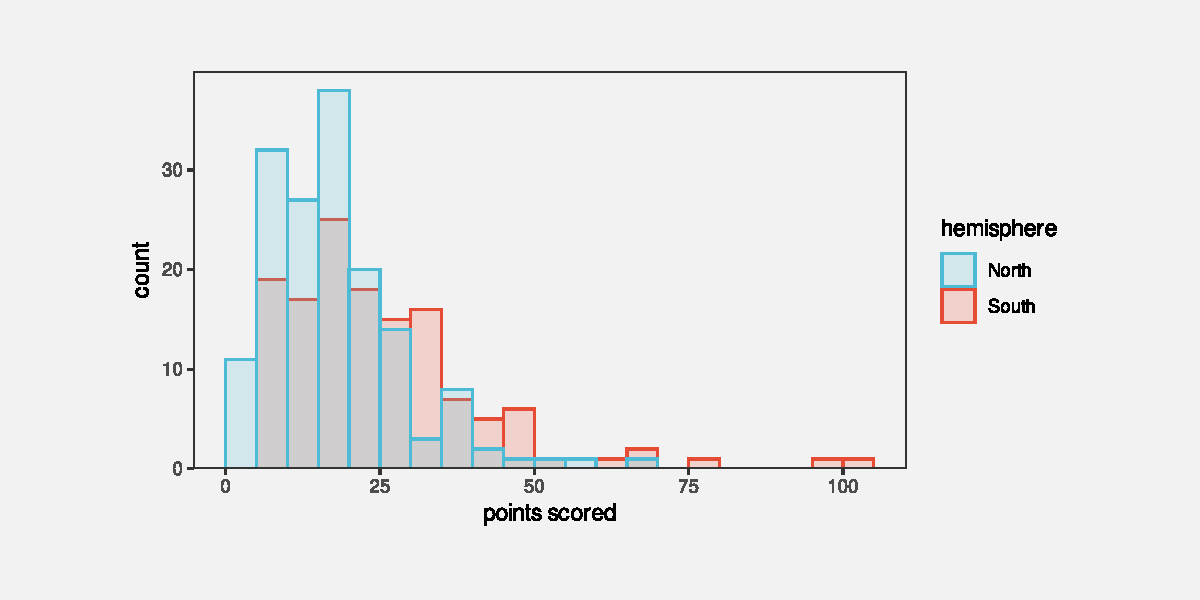
\includegraphics[width=1\linewidth,height=\textheight,keepaspectratio]{index_files/mediabag/visual-shapes_files/figure-pdf/fig-multiple-hist-1.pdf}

}

\caption{\label{fig-multiple-hist}Histograms of the points scored per
game by Tier One nations at Rugby World Cups, broken down by
hemisphere.}

\end{figure}%

\section{Aspect ratio}\label{aspect-ratio}

How aspect ratio affects ability to detect features in lines

Also use of white space around points in scatter plot ?

Cite Cleveland (1994) for white space margin affecting strength of
relation?

\section{The dangers of visual
shapes}\label{the-dangers-of-visual-shapes}

Need a caveat that more complex shapes does NOT necessarily mean useful
mappings back to data summaries - could just end up with a mess
(Figure~\ref{fig-data-vis-shape-lie}).

\begin{figure}

\centering{

\begin{figure}[H]

\begin{minipage}{0.50\linewidth}
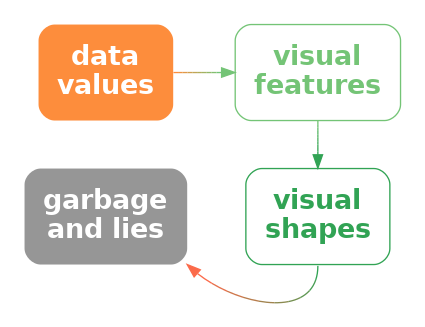
\includegraphics[scale=0.5]{Diagrams/data-vis-shape-lie.png}\end{minipage}%

\end{figure}%

}

\caption{\label{fig-data-vis-shape-lie}Mapping data values to the visual
features of a complex shape may not be effective if the complex shape
decodes to unhelpful or misleading information.}

\end{figure}%

Lines imply continuity (at least) if not linear interpolation so do
example where connecting with lines not such a great idea.

\section{Case study: Violin plots}\label{case-study-violin-plots}

And other variations on boxplots

\begin{itemize}
\tightlist
\item
  Case study: SinaPlots
\end{itemize}

A SinaPlot is a nice combination of decode for raw data and for data
summary. \footnote{Sidiropoulos et al. (2018)} Figure~\ref{fig-sina} is
actually a combination of a SinaPlot and a violin plot.

\begin{figure}

\centering{

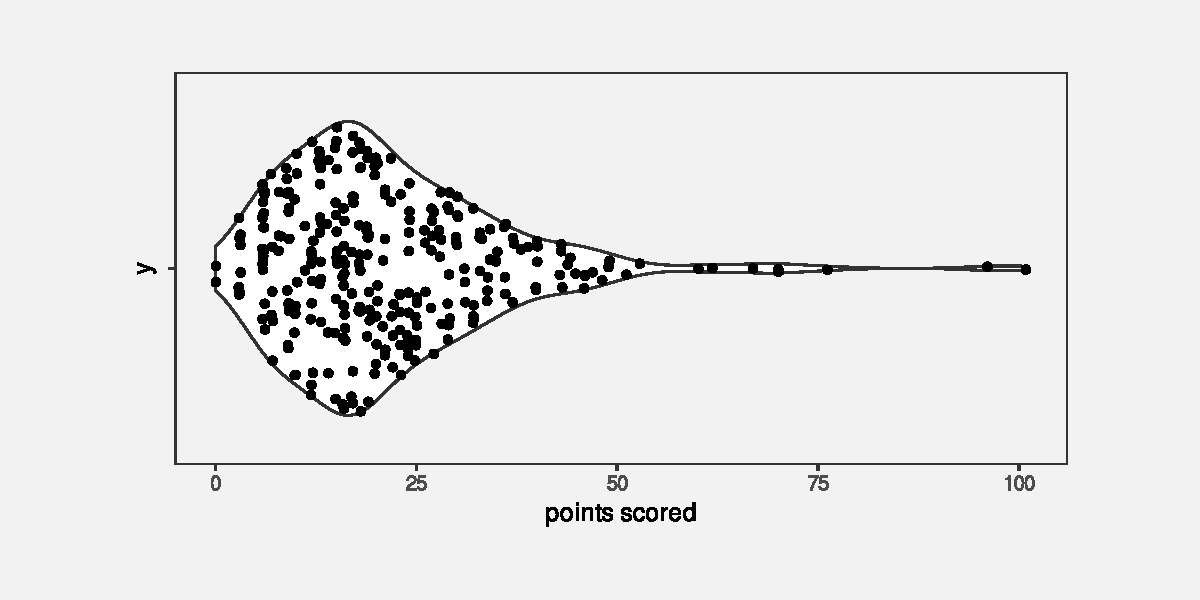
\includegraphics[width=1\linewidth,height=\textheight,keepaspectratio]{index_files/mediabag/visual-shapes_files/figure-pdf/fig-sina-1.pdf}

}

\caption{\label{fig-sina}A SinaPlot of the points scored per game by
Tier One nations at Rugby World Cups.}

\end{figure}%

\section{Case study: loess curves}\label{case-study-loess-curves}

Another example of data -\textgreater{} summary -\textgreater{} features
-\textgreater{} shapes -\textgreater{} summaries

\section{Case study: Line of best
fit}\label{case-study-line-of-best-fit}

Nice example of a complex calculation, the results of which are what
gets visualised. Also example of performing the calculation numerically
rather than asking the viewer to perform it visually. This was in
summaries.qmd, but it cannot be there because it requires scatter plots,
which come in the next section. Add this after mention of visualising
models?

Add footnote to Hadley's more complex model visualisation paper
https://vita.had.co.nz/papers/model-vis.pdf
https://dl.acm.org/doi/10.1002/sam.11271

model fits like lm straight line and ref Hadley's data-space vs
model-space ``data models'' to mirror ``data statistics'' (revisit box
plots as VERY simple models? also talk about failing assumptions of
these models, like unimodal for boxplot)

footnote cite to Tukey for visualising phenomena rather than raw data?
``Data-Based Graphics: Visual Display in the Decades to Come'' Tukey
(1990)

\section{Summary}\label{summary-9}

Mapping multiple data values to a single data symbol produces a
\textbf{visual shape}, like a line on a line plot.

Data summaries, such as trends over time, can can be decoded from a
visual shape. However, decoding raw data values from a visual shape may
be harder, cmopared to decoding raw data values from a simple data
symbol like a bar.

\begin{center}\rule{0.5\linewidth}{0.5pt}\end{center}

\theendnotes

\bookmarksetup{startatroot}

\chapter{Multiple Mappings}\label{multiple-mappings}

Figure~\ref{fig-multiple} shows a data visualisation of the performance
measures for teams in the 2023 Rugby World Cup
(Table~\ref{tbl-rwc-2023}). This visualisation is different from
anything we have seen previously because it involves multiple mappings.
The data symbol in this case is a simple data point, but we have mapped
data values to \emph{five} different visual features of each data point.
The number of clean breaks is encoded as the horizontal
\textbf{position} of the data points and the number of tries is encoded
as the vertical \textbf{position} of the data points. The number of
points scored is encoded as the \textbf{size} of the points, the
hemisphere is encoded as the \textbf{shape} of the points, and the
number of runs is encoded as the \textbf{colour} of the points.

\begin{figure}

\centering{

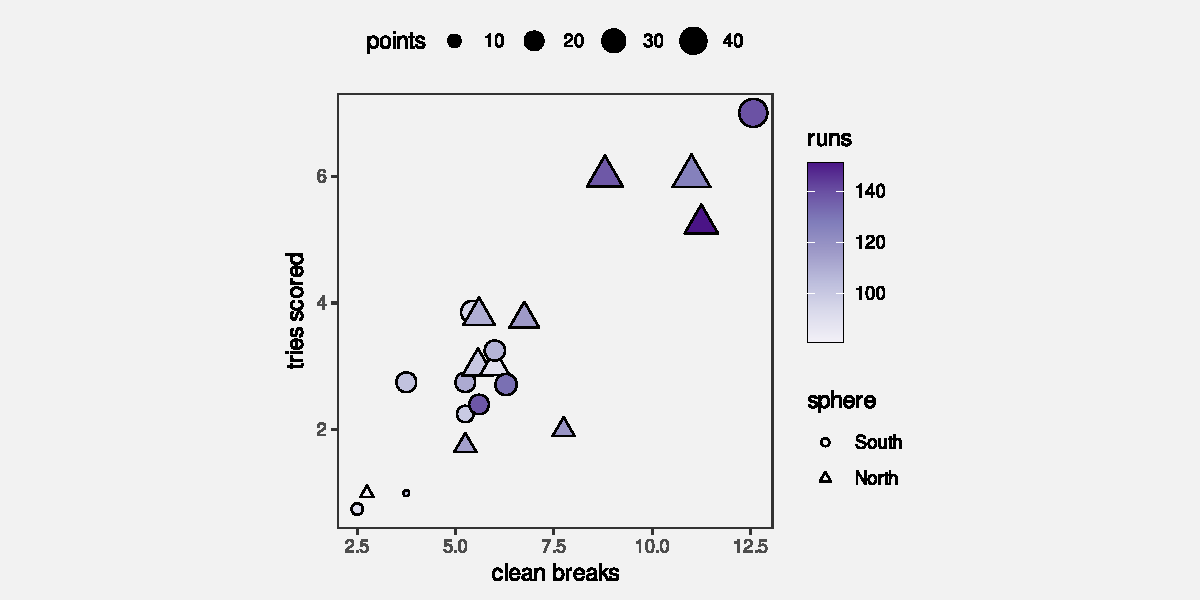
\includegraphics[width=1\linewidth,height=\textheight,keepaspectratio]{index_files/mediabag/multiple_files/figure-pdf/fig-multiple-1.pdf}

}

\caption{\label{fig-multiple}A data visualisation of the performance
measures for teams in the 2023 Rugby World Cup.}

\end{figure}%

Figure~\ref{fig-multiple} is effective in some ways because some of the
mappings involve effective visual features. For example, we can easily
decode the number of clean breaks and the number of tries from
horizontal and vertical positions. We can also decode a correlation
between clean breaks and tries from the emergent feature of
\textbf{position in space} (Section~\ref{sec-integral}).

However, other mappings are less effective. For example, it is less easy
to accurately decode number of points scored from size and even harder
to decode the number of runs from colour. In addition, we are hampered
by the fact that many different visual features are changing at once, so
it is harder to perceive individual differences (see
Section~\ref{sec-differences}).

One goal of visualising multiple variables like we have in
Figure~\ref{fig-multiple} is to discover or display multivariate
relationships between the variables. For example, we can see that there
are four teams in the top-right corner of the plot that are all
relatively large and relatively dark in colour, which suggests that
there is a group of teams that run more, make more clean breaks, score
more tries, and score more points compared to the other teams.

This section looks at some of the different approaches to visualising
several variables at once. How do we perceive multivariate
relationships? And can we still perceive individual data values at the
same time?

\section{Parallel coordinates plots}\label{sec-parallel}

One issue with Figure~\ref{fig-multiple} is that it attempts to map each
data variable to a separate visual feature. Once we have used both
horizontal and vertical \textbf{position}, we have to start using less
accurate and less appropriate visual features, like \textbf{area} and
\textbf{colour} for quantitative data values (see
Chapter~\ref{sec-mapping-visual-features}). If we attempted to map all
of the variables in Table~\ref{tbl-rwc-2023}, we could actually run out
of visual features to use (Figure~\ref{fig-visual-features}).

An alternative approach is to map more of the data variables to the same
visual feature. For example, Figure~\ref{fig-parallel} shows a parallel
coordinates plot of the data from Figure~\ref{fig-multiple}. In this
visualisation, all of the quantitative variables have been encoded as
\textbf{position}, with just hemisphere (qualitative) encoded as colour.

\begin{figure}

\centering{

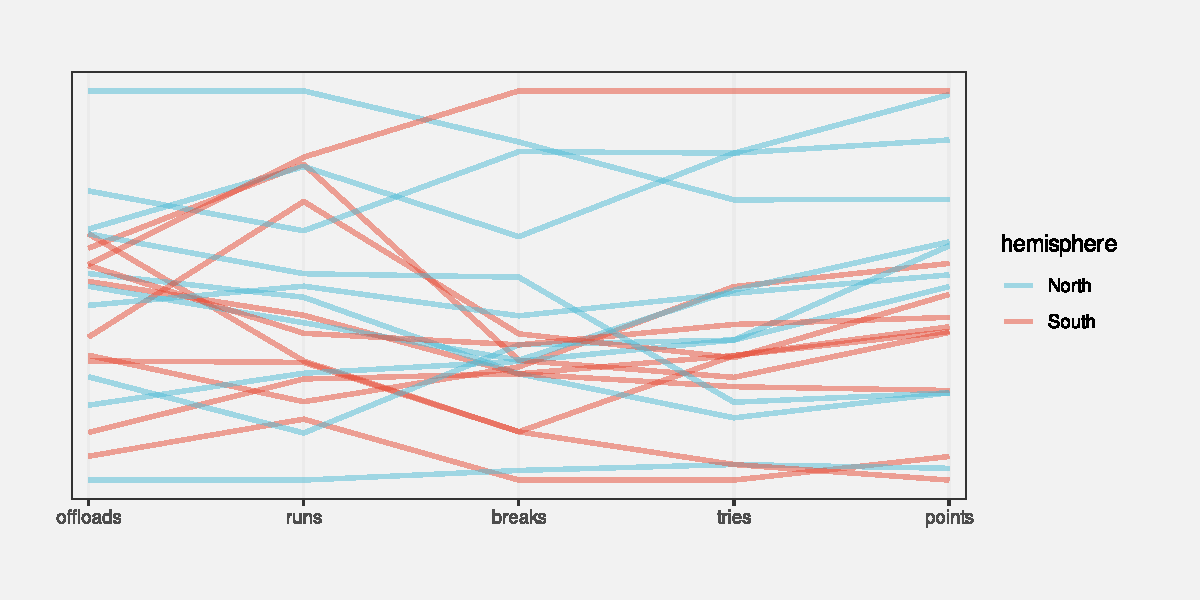
\includegraphics[width=1\linewidth,height=\textheight,keepaspectratio]{index_files/mediabag/multiple_files/figure-pdf/fig-parallel-1.pdf}

}

\caption{\label{fig-parallel}A data visualisation of the performance
measures for teams in the 2023 Rugby World Cup.}

\end{figure}%

A parallel coordinates plot maps data summaries rather than raw data
values (Chapter~\ref{sec-summaries}). For example, all data values are
standardised to a range between 0 and 1.\footnote{Acknowledge and point
  to different ways that the data values can be transformed (or
  summarised).} Table~\ref{tbl-parallel-stats} shows some of the values
that are actually mapped to visual features in
Figure~\ref{fig-parallel}. Each variable is encoded as a different
horizontal \textbf{position} and the values within each variable are
encoded as vertical \textbf{position}. In this way, all quantitative
data values are encoded as \textbf{position}.

\begin{longtable}[]{@{}lllr@{}}

\caption{\label{tbl-parallel-stats}The data summaries that are mapped to
visual features in Figure~\ref{fig-parallel}.}

\tabularnewline

\toprule\noalign{}
country & sphere & variable & value \\
\midrule\noalign{}
\endhead
\bottomrule\noalign{}
\endlastfoot
Namibia & South & runs & 0.16 \\
Romania & North & runs & 0.00 \\
Chile & South & runs & 0.30 \\
Samoa & South & runs & 0.31 \\
Australia & South & runs & 0.42 \\
Georgia & North & runs & 0.47 \\

\end{longtable}

In addition, the hemisphere is encoded as \textbf{colour} and a separate
line data symbol is drawn for each country. This means that a visual
shape is drawn for each country (Figure~\ref{fig-mappings-1-n-1-n};
Chapter~\ref{sec-visual-shapes}).

\begin{figure}

\begin{minipage}{0.50\linewidth}

\pandocbounded{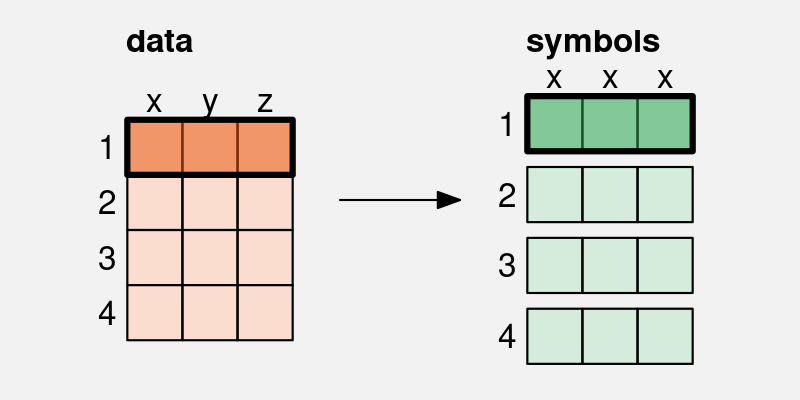
\includegraphics[keepaspectratio]{Mappings/mapping-1-n-1-n.png}}

\end{minipage}%

\caption{\label{fig-mappings-1-n-1-n}In a parallel coordinates plot, a
single row of data---one data value from each of several variables---is
mapped to a visual shape (a line).}

\end{figure}%

On one hand, a parallel coordinates plot appears to makes sense because
it encodes multiple data values to \textbf{position}, which is an
accurate visual feature for quantitative data. However, this advantage
is immediately squandered because the values that are encoded are not
the raw data values (Figure~\ref{fig-stat-vis-decode}), so a parallel
coordinates plot is not effective for decoding raw data values from the
positions of the lines. Furthermore, the data symbols are lines, so each
data symbol encodes multiple data values (Section~\ref{sec-line-plots}),
which makes it difficult to decode even individual data summary values
from the lines.

The effectiveness of a parallel coordinates plot comes from the visual
shapes produced by the lines. For example, in Figure~\ref{fig-parallel},
we are able to identify a group of four lines at the top of the plot
that are separate from the other lines. This grouping across at least
three variables (clean breaks, tries, and points) is easier to see
compared to Figure~\ref{fig-multiple}. We can also more clearly see that
there are two teams that have similar numbers of runs to the top four,
but then are mixed in with the other teams on the other variables.
Furthermore, the fact that many of the lines are reasonably horizontal
rather than criss-crossing each other wildly suggests that there is an
overall correlation between all four quantitative variables, not just in
the top four teams.

\begin{quote}
A parallel coordinates plot can be effective at identifying
high-dimensional groups or correlations because it maps multiple data
values from different variables to a single visual shape.
\end{quote}

\section{Case study: Bubble plots}\label{case-study-bubble-plots}

An example of using area/size for third variable.

Provide some better options.

\section[Small multiples]{\texorpdfstring{Small
multiples\footnote{Tufte's small multiples}}{Small multiples}}\label{small-multiplessmall-multiples}

One difficulty with Figure~\ref{fig-parallel} is that many of the lines
overlap each other, which makes it difficult to separately perceive
individual visual shapes. Figure~\ref{fig-profile} shows an alternative
approach to visualising the same data, called a profile plot. Similar to
a parallel coordinates plot, a visual shape is drawn for each country,
but the shape in this case is a filled in polygon, effectively the lines
in Figure~\ref{fig-parallel} with the area below them (down to zero)
filled in.

Again, this sort of data visualisation can be effective because of the
overall shapes. For example, we can see a group of four shapes that are
larger than the others. We can also see that Argentina and Fiji appear
very similar, which was not apparent in previous plots.

\begin{figure}

\centering{

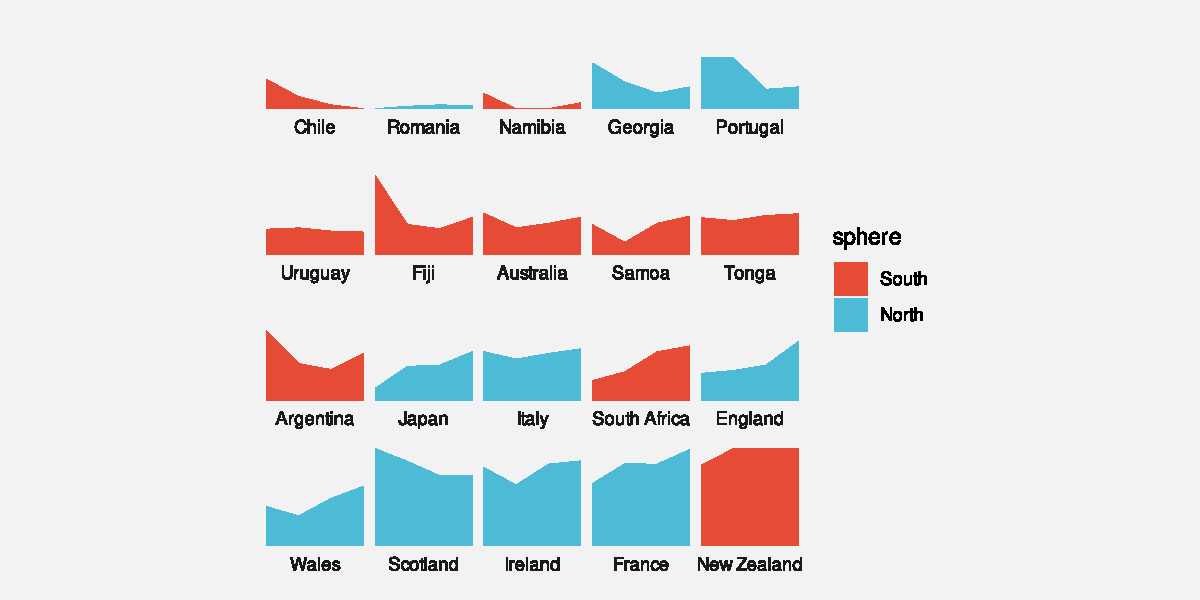
\includegraphics[width=1\linewidth,height=\textheight,keepaspectratio]{index_files/mediabag/multiple_files/figure-pdf/fig-profile-1.pdf}

}

\caption{\label{fig-profile}A data visualisation of the performance
measures for teams in the 2023 Rugby World Cup.}

\end{figure}%

Figure~\ref{fig-profile} uses the same data summaries as
Figure~\ref{fig-parallel} (Table~\ref{tbl-parallel-stats}), and similar
mappings: each variable is encoded as a different horizontal
\textbf{position} and the values within each variable are encoded as
vertical \textbf{position} and hemisphere is mapped to \textbf{colour}.
The data symbol is also similar: multiple data values are mapped to a
single data symbol, in this case a polygon.

The difference in Figure~\ref{fig-profile} is that, rather than having
all of the data symbols on the same plot, each data symbol is drawn in
its own \textbf{position in space}. This makes it easy to view each
distinct data symbol.

The cluster of four larger shapes in Figure~\ref{fig-profile} is also
easier to see because the countries have been ordered by the number of
points scored (the right-hand height of the shape). As we have seen
before, ordering data symbols can make a big difference
(Section~\ref{sec-distance-effect}).

\section[Facetting]{\texorpdfstring{Facetting\footnote{trellis
  multi-panels, ggplot2 facets, GoG ??}}{Facetting}}\label{sec-facetting}

Figure~\ref{fig-facet-before} shows a line plot of the number of youth
offenders per year in different Police Districts of New Zealand. This
visualisation makes use of several effective mappings. For example, we
encode year as horizontal \textbf{position} and we encode count as
vertical \textbf{position}. However, there is also a weaker mapping: the
Police District. We encode districts as \textbf{colour}, but because
there are 12 different districts, we are exceeding the capacity of
colour (Section~\ref{sec-capacity}). It is not easy to differentiate all
of the different colours (not helped by overplotting of the lines).

A better mapping for Police District would be \textbf{position}, which
has a much higher capacity, but position has already been taken by year
and count.

\begin{figure}

\centering{

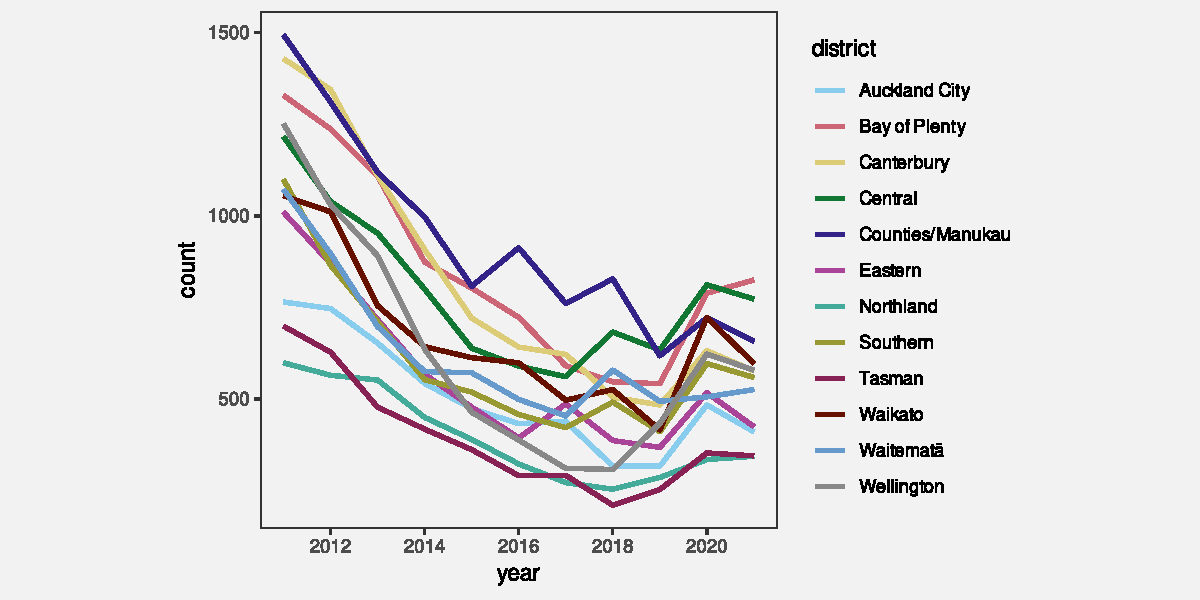
\includegraphics[width=1\linewidth,height=\textheight,keepaspectratio]{index_files/mediabag/multiple_files/figure-pdf/fig-facet-before-1.pdf}

}

\caption{\label{fig-facet-before}A data visualisation of the number of
offenders per year in different Police Districts of New Zealand, from
2011 to 2021.}

\end{figure}%

Figure~\ref{fig-facet-after} shows one solution: a facetted plot. Each
district has been encoded as a \textbf{position in space} and we draw a
separate plot for each district. This makes it very easy to distinguish
the individual districts.

One downside is that comparisons between districts are more difficult
because counts and/or years are \textbf{unaligned}
(Section~\ref{sec-unaligned-pos}). In this case, we have mitigated that
problem by drawing a grey line for all districts in each plot. Similar
to grid lines, this makes it easier to compare the line for each
district to other districts (Section~\ref{sec-perception-relative}).

\begin{figure}

\centering{

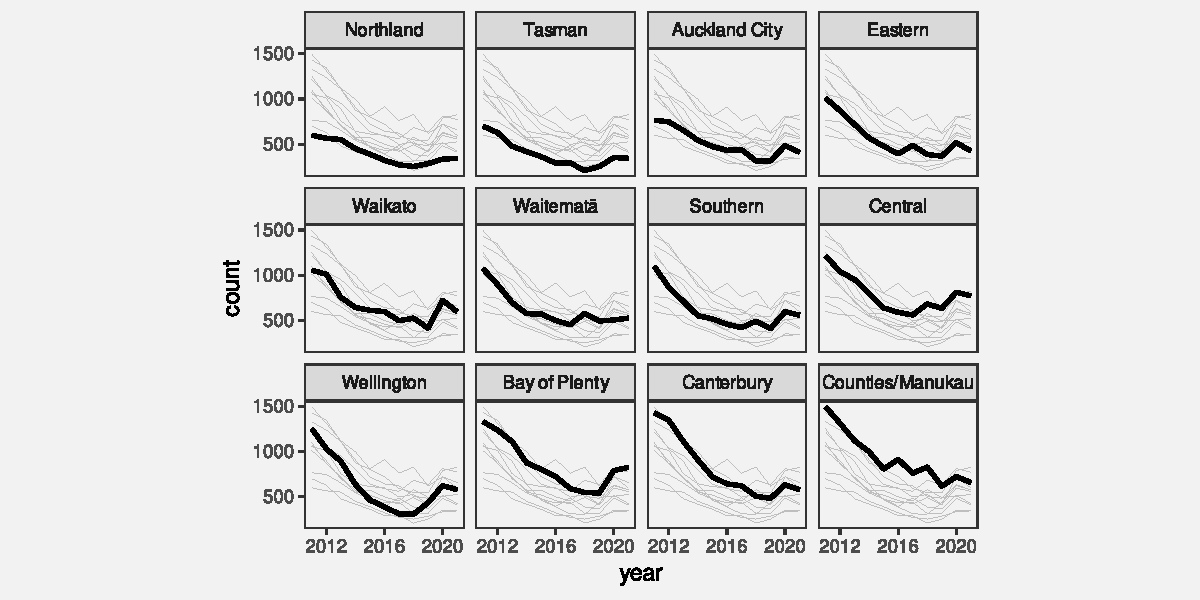
\includegraphics[width=1\linewidth,height=\textheight,keepaspectratio]{index_files/mediabag/multiple_files/figure-pdf/fig-facet-after-1.pdf}

}

\caption{\label{fig-facet-after}A data visualisation of the number of
offenders per year in different Police Districts of New Zealand, from
2011 to 2021.}

\end{figure}%

We have again ordered the panels so that districts are near to other
districts with a similar starting count of offenders
(Section~\ref{sec-distance-effect}).

\section{Case study: Scatterplot
matrices}\label{case-study-scatterplot-matrices}

Figure~\ref{fig-splom} shows a scatter plot matrix of the performance
measures for teams in the 2023 Rugby World Cup
(Table~\ref{tbl-rwc-2023}).

This is another example of reusing \textbf{position} to encode data
values. Each combination of variables is encoded as a separate scatter
plot at a different position in space and, within each scatter plot, two
variables are encoded as horizontal and vertical position.

Within each scatter plot, there is an emergent feature of position in
space, which allows us to decode the correlation between different pairs
of variables. Although this only allows us to see pairwise correlations
between variables, we can also get a glimpse of higher-level
correlations across several of the scatterplots.

For example, looking down the diagonal of the matrix, we can see that:
the number of runs is correlated loosely with the number of clean
breaks; the number of clean breaks is more strongly correlated with the
number of tries; and the number of tries is very strongly correlated
with the number of points.

If we look down the first column of the matrix, we can see that: the
number of runs is correlated loosely with the number of clean breaks, a
little more loosely with the number of tries and a little more loosely
still with the number of points.

\begin{figure}

\centering{

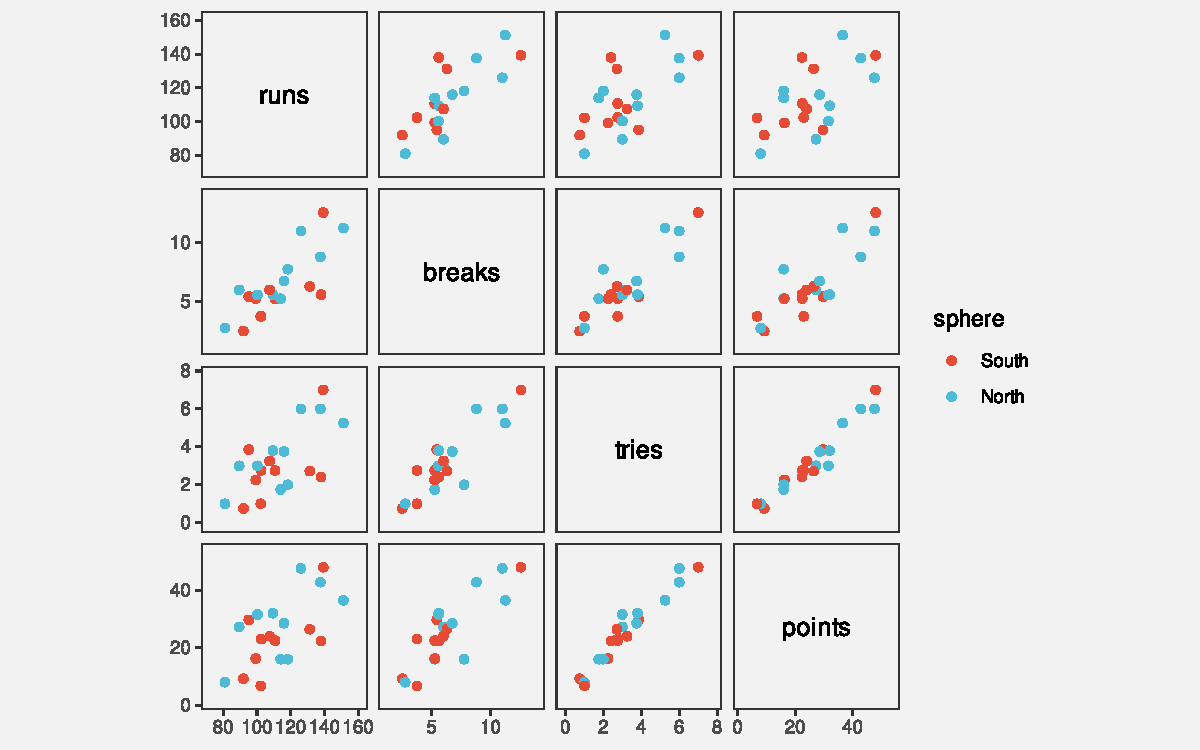
\includegraphics[width=1\linewidth,height=\textheight,keepaspectratio]{index_files/mediabag/multiple_files/figure-pdf/fig-splom-1.pdf}

}

\caption{\label{fig-splom}A scatter plot matrix of the quantitative
performance measures for teams in the 2023 Rugby World Cup.}

\end{figure}%

\section{Non-cartesian mappings}\label{non-cartesian-mappings}

Parallel plots is actually an example of this, so can just refer back to
Section~\ref{sec-parallel}

Refer back to Section~\ref{sec-non-linear}

\section{Case study: kiviat plots or radar plots or spider
plots}\label{case-study-kiviat-plots-or-radar-plots-or-spider-plots}

(David Peebles (2008))

\section{Case study: Barycentric plots (ternary
plots)}\label{case-study-barycentric-plots-ternary-plots}

\section{Dangers of multiple
mappings}\label{dangers-of-multiple-mappings}

Figure~\ref{fig-multiple} showed that the naive approach of just using a
separate visual feature for each data variable leads to complex data
visualisations that are difficult to decode. Although there are better
options, like small multiple and facetting, there is still a limit to
how much information can effectively be displayed at once within a
static data visualisation.

This is one area where dynamic and interactive graphics can be useful
because the viewer is able to rapidly switch between multiple views of
the data, which means that each individual view can be
simpler.\footnote{Cite again the classic interactive lit ? Point to some
  tools that might help, like GGobi?}

\section{Summary}\label{summary-10}

When we need to visualise multiple variables at once, it is not
effective to map each different variable to a different visual feature.

An alternative is to reuse the same visual feature for multiple
different variables. In particular, small multiples, or facetting,
allows us to use \textbf{position} for more than just two variables.

\begin{center}\rule{0.5\linewidth}{0.5pt}\end{center}

\theendnotes

\bookmarksetup{startatroot}

\chapter{Visual Objects}\label{visual-objects}

Figure~\ref{fig-scatter-country} shows a scatter plot of the number of
clean breaks and the number of tries for countries at the 2023 Rugby
World Cup (Table~\ref{tbl-rwc-2023}). This data visualisation is similar
to Figure~\ref{fig-scatter}, but it adds an extra mapping. Country names
are encoded as the \textbf{shape} of the data symbols. This is a
reasonable mapping, despite the large number of different countries,
because each different shape only appears once. We are able to
distinguish all countries from each other and, thanks to the legend, we
can identify individual countries.

\begin{figure}

\centering{

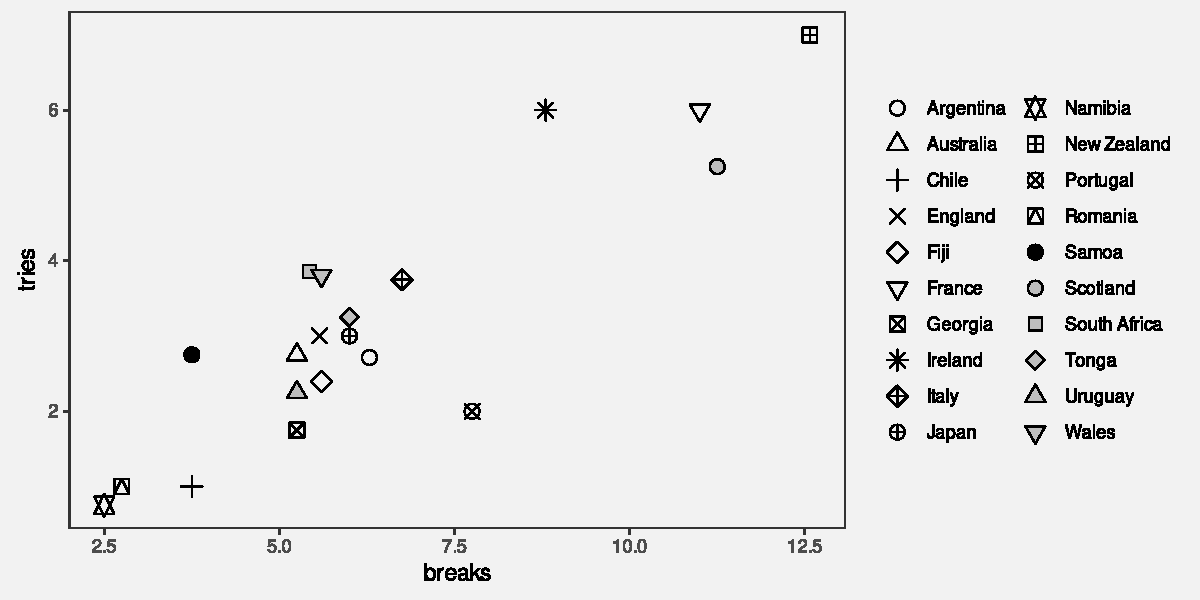
\includegraphics[width=1\linewidth,height=\textheight,keepaspectratio]{index_files/mediabag/visual-objects_files/figure-pdf/fig-scatter-country-1.pdf}

}

\caption{\label{fig-scatter-country}A scatter plot with a different
shape per country}

\end{figure}%

Figure~\ref{fig-flags} shows another scatter plot of the number of clean
breaks and the number of tries for countries at the 2023 Rugby World
Cup, but this time with flags as the data symbols. In one sense, this is
just a variation on Figure~\ref{fig-scatter-country} because the country
names are encoded as the \textbf{shape} of a data symbol. Each data
symbol is a shape that allows us to distinguish between the different
countries.

The difference between the data symbols in
Figure~\ref{fig-scatter-country} and the data symbols on
Figure~\ref{fig-flags} is that the flags are not only more complicated
shapes, but they are familiar shapes. The flags convey differences, but
they also convey the more sophisticated concept of the country names. In
the terms of Section~\ref{sec-visual-processing}, the flags are
\textbf{visual objects} that might take longer to process, but convey
more information.

\begin{figure}

\centering{

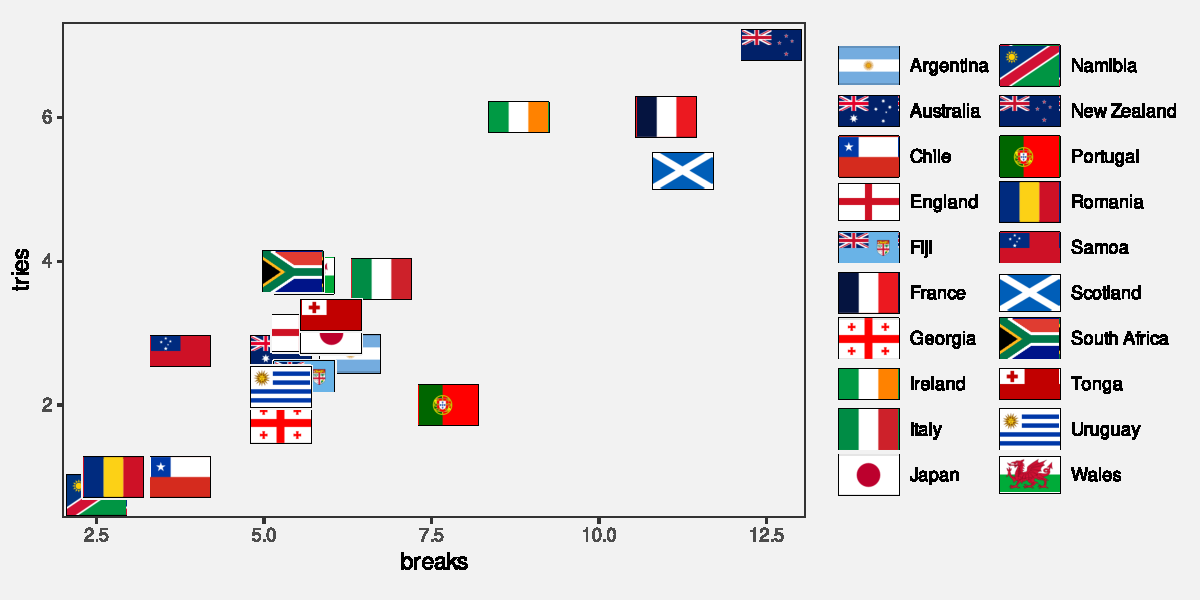
\includegraphics[width=1\linewidth,height=\textheight,keepaspectratio]{index_files/mediabag/visual-objects_files/figure-pdf/fig-flags-1.pdf}

}

\caption{\label{fig-flags}A scatter plot with flags as data symbols}

\end{figure}%

\section{Learned mappings}\label{sec-learned}

We \textbf{encode} data values as visual features so that the viewers of
a data visualisation can \textbf{decode} the data values from the visual
features (Figure~\ref{fig-visual-feature-decode}).

In Section~\ref{sec-implicit}, we saw that some encodings are effective
because there are implicit decodings. For example, a longer bar in a bar
plot naturally corresponds to a larger quantity. Basic visual features,
like length, are effective thanks to \textbf{pre-existing} decodings
that are built-in features of our visual system.

Part of the power of visual objects also comes from
\textbf{pre-existing} decodings. However, these decodings are
\textbf{learned} rather than being built-in. In some cases, we are able
to \textbf{decode} values from a visual feature based on prior
experience and learning, rather than due to an explicit encoding
(Figure~\ref{fig-learned-decode}).\footnote{``Mapping Color to Meaning
  in Colormap Data Visualizations'' Schloss et al (2018) They call this
  an ``inferred mapping''}

\begin{figure}

\centering{

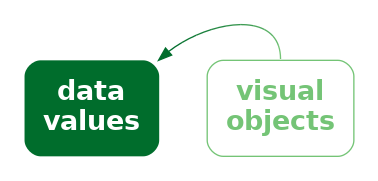
\includegraphics[scale=0.5]{Diagrams/learned-decode.png}

}

\caption{\label{fig-learned-decode}Some visual features have learned
encodings, which means that we can decode values from the visual
features without having explicitly encoded values as visual features.}

\end{figure}%

For example, Figure~\ref{fig-learned} shows three coloured circles.
Without any explicit encoding, we can decode the red circle as ``stop'',
the orange circle as ``slow'', and the green circle as ``go''. This is
not a decoding that we are born with; it is a decoding that we learn
through experience.

\begin{figure}

\centering{


\includegraphics[width=1\linewidth,height=\textheight,keepaspectratio]{index_files/mediabag/visual-objects_files/figure-pdf/fig-learned-1.pdf}

}

\caption{\label{fig-learned}An example of visual symbols that have
pre-existing, learned decodings.}

\end{figure}%

The flags in Figure~\ref{fig-flags} provide examples of learned
decodings. We associate each flag with a particular country because we
have seen these flags before and they have learned the decoding from
flag to country. Figure~\ref{fig-flags-direct} demonstrates this point
by repeating the scatter plot, but removing the legend. We are still
able to identify not only that the data symbols represent different
countries, but we can identify (at least some of) the country names as
well.

\begin{figure}

\centering{

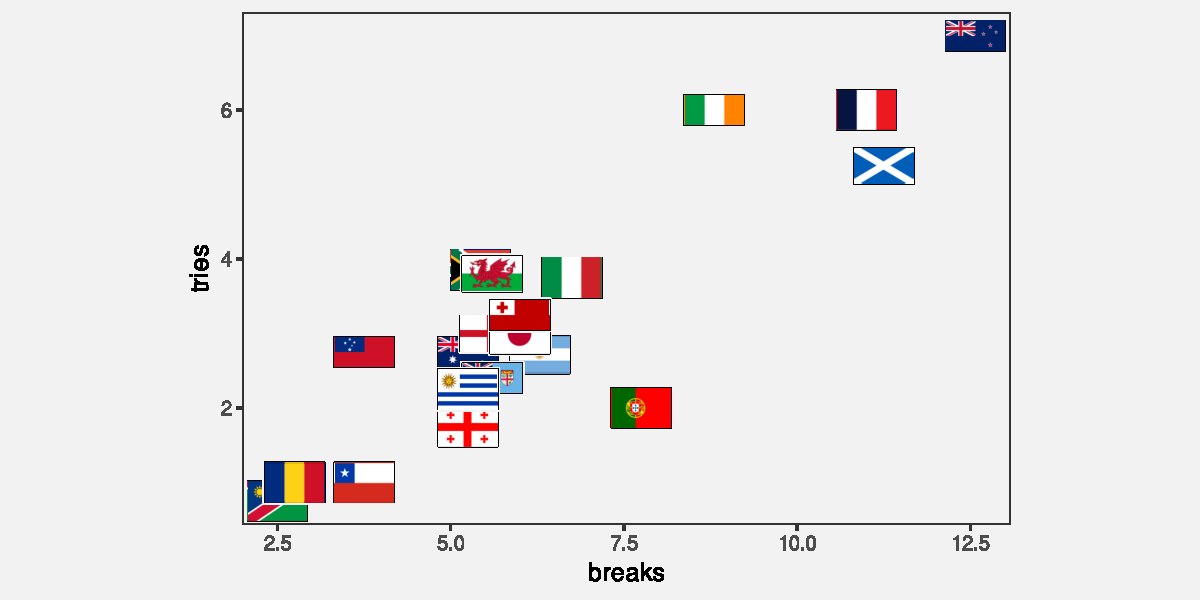
\includegraphics[width=1\linewidth,height=\textheight,keepaspectratio]{index_files/mediabag/visual-objects_files/figure-pdf/fig-flags-direct-1.pdf}

}

\caption{\label{fig-flags-direct}A scatter plot with flags as data
symbols}

\end{figure}%

Just to make the point completely clear,
Figure~\ref{fig-scatter-country-no-legend} shows
Figure~\ref{fig-scatter-country} without a legend. Although we can still
perceive that the data symbols are different from each other, there is
nothing about the shape of the data symbols in
Figure~\ref{fig-scatter-country-no-legend} that conveys the country
names. We can clearly see that Figure~\ref{fig-flags-direct} contains
more information than Figure~\ref{fig-scatter-country-no-legend}.

\begin{figure}

\centering{

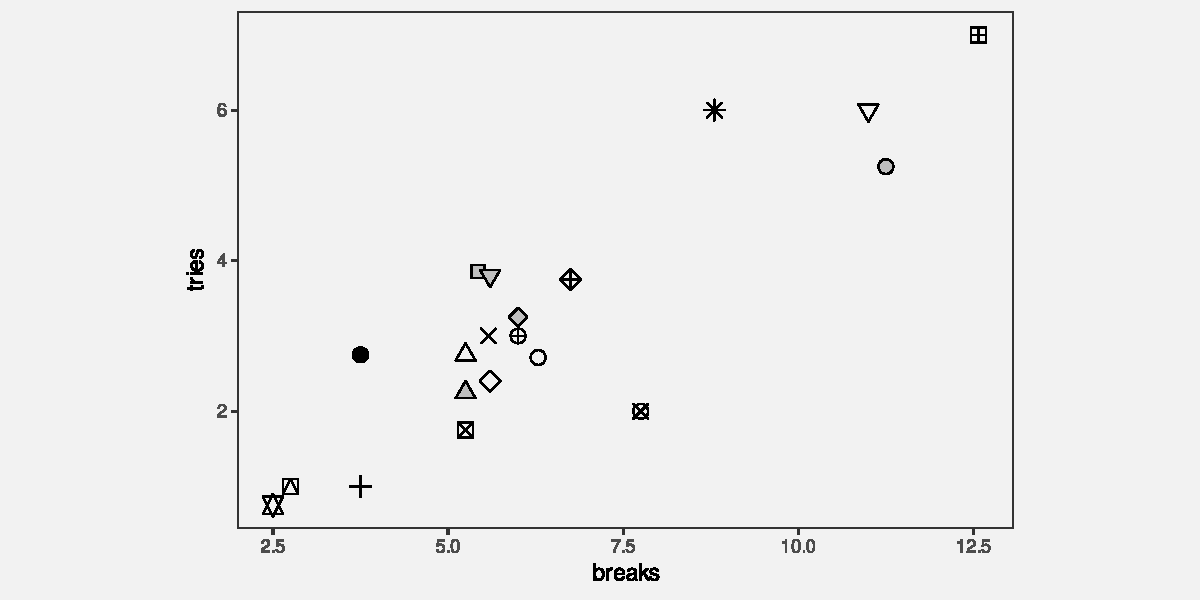
\includegraphics[width=1\linewidth,height=\textheight,keepaspectratio]{index_files/mediabag/visual-objects_files/figure-pdf/fig-scatter-country-no-legend-1.pdf}

}

\caption{\label{fig-scatter-country-no-legend}A scatter plot with a
different shape per country}

\end{figure}%

\begin{quote}
A plot that uses visual objects as data symbols can be effective because
the visual objects can convey information based on learned associations.
\end{quote}

Figure~\ref{fig-flags-direct} also demonstrates a weakness of
\textbf{visual objects}. The flags work well for identifying the country
names \emph{only if} we are familiar with all of the different flags.
For example, it may only be Australians and New Zealanders who can
reliably identify the difference between their two flags.

\begin{quote}
A plot that uses visual objects as data symbols may \emph{not} be
effective if the learned associations are not widely known.
\end{quote}

\section{Case study: Choropleth maps}\label{sec-choropleth}

Figure~\ref{fig-map} shows a choropleth map of the average crime rate,
over the period from 2011 to 2021, in each police district of New
Zealand.\footnote{Add citations to MacEachren and Bertin and Dan Carr ?}
The data values for this map are shown in Table~\ref{tbl-map-data}.

\begin{longtable}[]{@{}lr@{}}

\caption{\label{tbl-map-data}The average crime rate over the period 2011
to 2021 for each police district of New Zealand.}

\tabularnewline

\toprule\noalign{}
district & rate \\
\midrule\noalign{}
\endhead
\bottomrule\noalign{}
\endlastfoot
Auckland City & 0.32 \\
Bay of Plenty & 0.62 \\
Canterbury & 0.38 \\
Central & 0.56 \\
Counties/Manukau & 0.39 \\
Eastern & 0.66 \\
Northland & 0.61 \\
Southern & 0.49 \\
Tasman & 0.62 \\
Waikato & 0.46 \\
Waitematā & 0.28 \\
Wellington & 0.33 \\

\end{longtable}

The data symbol in Figure~\ref{fig-map} is a polygon representing the
geographic boundary of each police district. This implicitly entails an
encoding of a police district as the \textbf{position} of a polygon.
Crime rate is encoded as the fill colour of each polygon.

The use of polygons as data symbols is effective because the polygons
form familiar shapes with familiar spatial arrangements (familiar to a
New Zealand audience at least). The polygons are \textbf{visual objects}
that convey the concepts of districts within New Zealand. The spatial
arrangements are also a form of visual \textbf{congruence}; the
arrangements mirror the real-world spatial relationships between the
regions (see Chapter~\ref{sec-congruence}).

\begin{figure}

\centering{

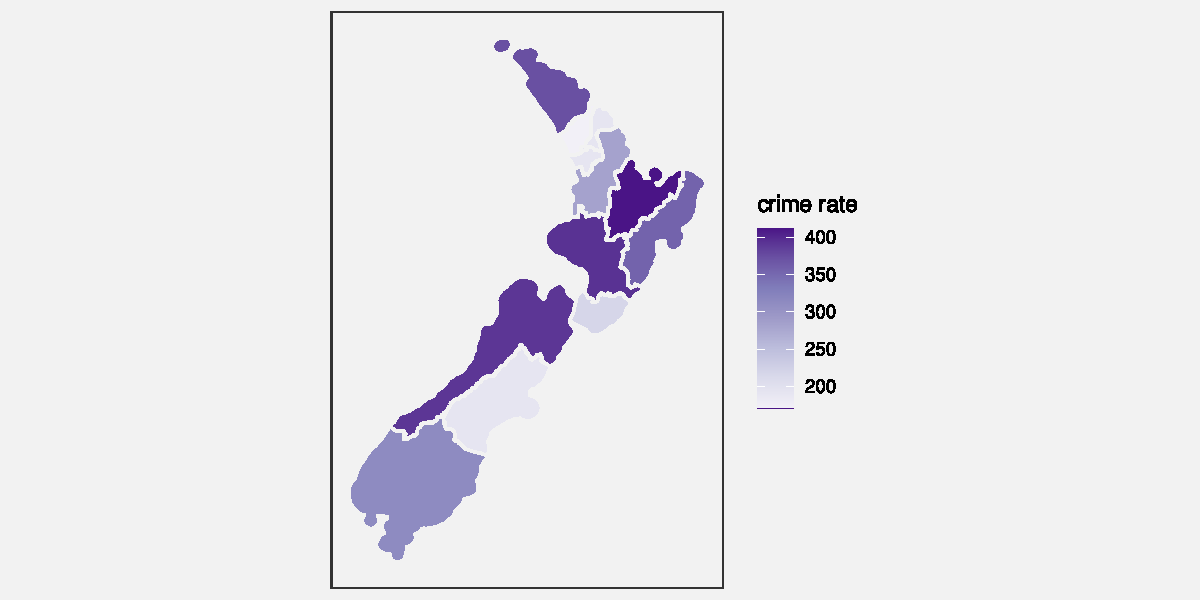
\includegraphics[width=1\linewidth,height=\textheight,keepaspectratio]{index_files/mediabag/visual-objects_files/figure-pdf/fig-map-1.pdf}

}

\caption{\label{fig-map}A choropleth map of the average crime rate over
the period 2011 to 2021 for each police district.}

\end{figure}%

\begin{quote}
A choropleth map is effective because it maps geographic regions to
familiar visual objects that resemble the real world regions.
\end{quote}

A weakness of Figure~\ref{fig-map} is that it encodes the
\textbf{quantitative} crime rate as colour (chroma and/or luminance).
This means that we can only decode ordinal comparisons between regions
(see Section~\ref{sec-ordinal}). For example, we can see that the
highest crime rate occurs in the district to the east of the North
Island, but it is difficult to perceive how much higher that crime rate
is compared to the next highest crime rate.

\begin{quote}
A choropleth map is \emph{only} effective for making ordinal comparisons
between geographic regions because it encodes quantitative values as
colour.
\end{quote}

Figure~\ref{fig-district-bar} shows a bar plot of the same data, which
demonstrates the advantages and disadvantages of the choropleth map in
Figure~\ref{fig-map}. In Figure~\ref{fig-district-bar}, it is much
easier to compare the crime rate values because crime rates are encoded
as bar \textbf{length}. However, it is much harder to associate the
different regions with their spatial arrangements because all we have
are the region names. Each police district is encoded as the vertical
position of a bar, with no correspondence to the spatial arrangement of
the regions in the real world.

\begin{figure}

\centering{

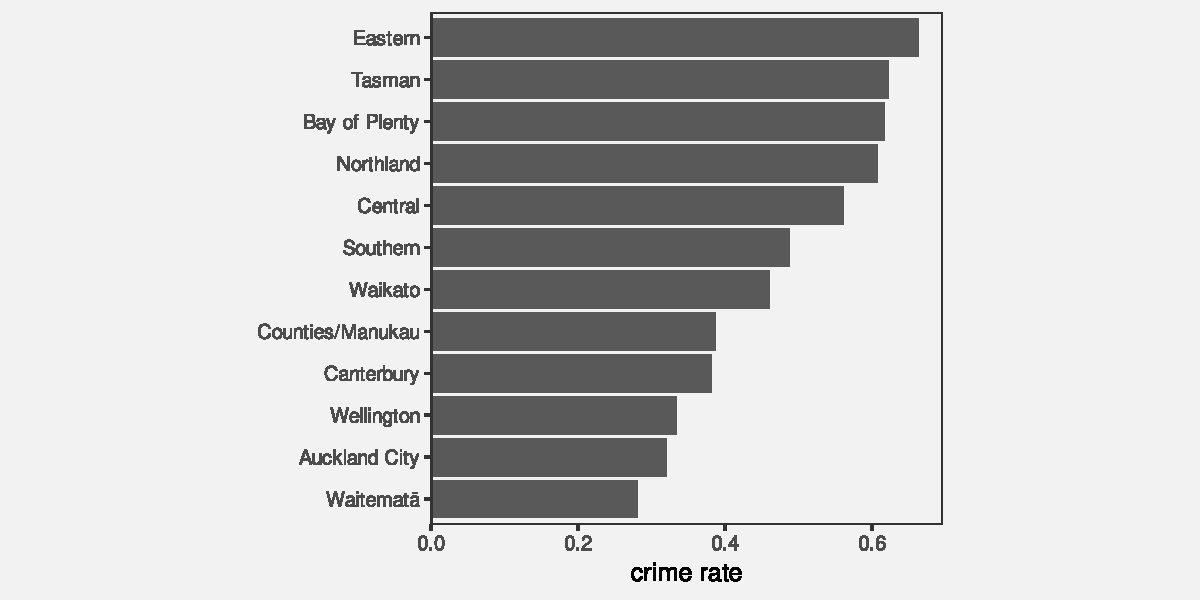
\includegraphics[width=1\linewidth,height=\textheight,keepaspectratio]{index_files/mediabag/visual-objects_files/figure-pdf/fig-district-bar-1.pdf}

}

\caption{\label{fig-district-bar}}

\end{figure}%

Another potential weakness with choropleth maps is the fact that regions
differ in terms of \textbf{area}. We know from
Section~\ref{sec-more-is-more} that larger data symbols are associated
with larger data values. The larger polygons accurately reflect the fact
that some police districts are geographically larger than others, but
there is potential for larger polygons to be erroneously decoded as
larger crime rates.

Two alternative approaches are shown in Figure~\ref{fig-map-alt}. These
both retain the region shapes of the map, but map crime rates to the
\textbf{area} of circles or the \textbf{length} of bars. These data
symbols have a spatial arrangement that corresponds to the real-world
arrangement of police districts and they provide a better decoding of
crime rates from data symbols compared to the colours in the choropleth
map (although area is still not the most accurate visual feature and the
lengths are unaligned; see Section~\ref{sec-accuracy}).

\begin{figure}

\begin{minipage}{0.50\linewidth}

\centering{

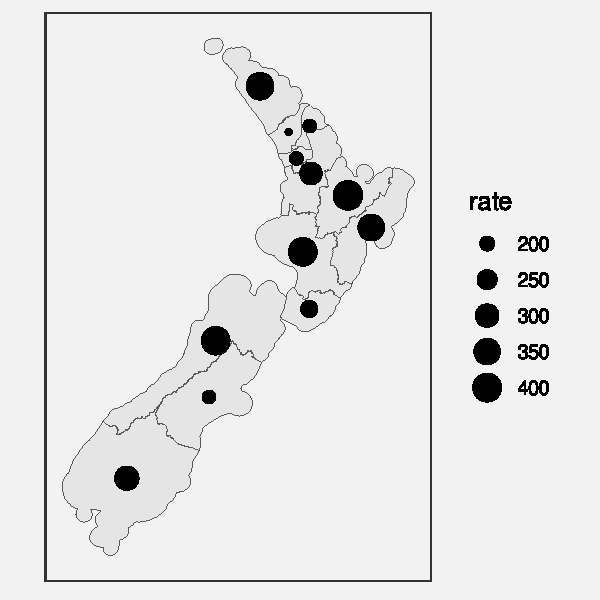
\includegraphics[width=1\linewidth,height=\textheight,keepaspectratio]{index_files/mediabag/visual-objects_files/figure-pdf/fig-map-alt-1.pdf}

}

\subcaption{\label{fig-map-alt-1}Dots as data symbols.}

\end{minipage}%
%
\begin{minipage}{0.50\linewidth}

\centering{

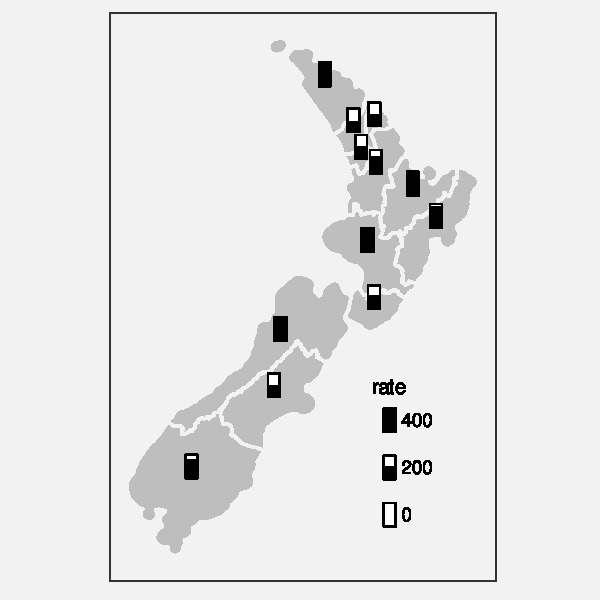
\includegraphics[width=1\linewidth,height=\textheight,keepaspectratio]{index_files/mediabag/visual-objects_files/figure-pdf/fig-map-alt-2.pdf}

}

\subcaption{\label{fig-map-alt-2}Bars as data symbols.}

\end{minipage}%

\caption{\label{fig-map-alt}Alternative map-based representations of the
average crime rate over the period 2011 to 2021 for each police
district.}

\end{figure}%

\section{Chart junk and clutter}\label{sec-junk}

Figure~\ref{fig-junk} shows a version of Figure~\ref{fig-map} with two
cartoon villians added in the top-left and bottom-right
corners.\footnote{Attribution for the original public domain image.}
These sorts of annotations are often, derisively, referred to as
\textbf{chart junk}, with the suggestion that they add no value and make
it harder to extract the important information.\footnote{Mention Tufte
  (data-ink ratio), Stephen Few? see DataVis/README for links to the
  debate.

  \begin{itemize}
  \tightlist
  \item
    ``Declutter and Focus: Empirically Evaluating Design Guidelines for
    Effective Data Communication'' Ajani et al (2021) says that ``The
    visualization practitioner community prescribes two popular
    guidelines for creating clear and efficient visualizations:
    declutter and focus.''
  \end{itemize}}

\begin{figure}

\centering{

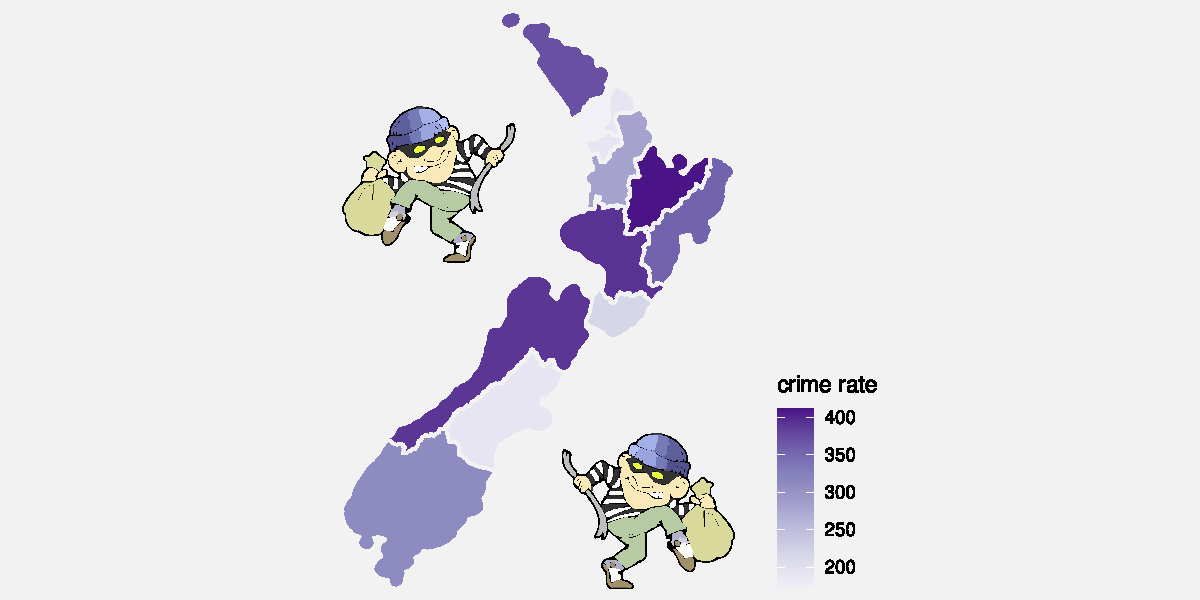
\includegraphics[width=1\linewidth,height=\textheight,keepaspectratio]{index_files/mediabag/visual-objects_files/figure-pdf/fig-junk-1.pdf}

}

\caption{\label{fig-junk}A choropleth map of the average crime rate over
the period 2011 to 2021 for each police district (like
Figure~\ref{fig-map}), with cartoon villian images added.}

\end{figure}%

The cartoon villians are an example of \textbf{visual objects}. They
(crudely) convey the concepts of crime and criminals. However, they are
\emph{not} \textbf{data symbols} because there is no mapping from the
raw data to the cartoon villians. Their position is unrelated to the
data, their colour is unrelated to the data, and their size is unrelated
to the data. The best that can be said is that they relate to the
\textbf{metadata}, the general topic of the data visualisation.
Annotations like this are closer in purpose to \textbf{labels} (see
Section~\ref{sec-labels}).

In Section~\ref{sec-differences} we learned that we should keep things
simple and only present visual changes that correspond to changes in the
data. In Section~\ref{sec-attention} we learned that our attention is
drawn to the larger and brighter items within an image. The cartoon
villians are relatively large, complex, and colourful and bear no
connection to the raw data, so there is a good chance that they will
distract from the visual features that do convey data values.

\begin{quote}
Chart junk is \emph{not} effective because it is impossible to decode
data values from chart junk (no data values have been encoded) and
because chart junk distracts from the visual elements that do represent
data values.
\end{quote}

However, it is important to point out that not all \textbf{visual
objects} are chart junk. For example, the data symbols in
Figure~\ref{fig-junk}, the map regions, are also \textbf{visual
objects}, but they differ from the cartoon villians because they are
related to the data values.

Furthermore, \textbf{visual objects} that have no connection to the raw
data may still have some positive effects. For example, the cartoon
villians are not devoid of information; they convey the concept of crime
more dramatically than the simple text label ``crime rate''. The more
complex and interesting images may attract attention to the data
visualisation as a whole and there is some evidence that such
annotations improve the memorability of a data visualisation.\footnote{Links
  to studies that try to show benefits of chart junk. Rahman et al
  (2024) Mention affect (emotion) study?}

\begin{quote}
Chart junk can be effective because it has a greater emotional impact
and is more memorable.
\end{quote}

Overall, visual objects that are not related to data values are
\emph{not} effective for decoding data values, so any other benefits
have to be weighed against that cost.\footnote{There is a really nice
  summary of when chart junk might be acceptable somewhere in
  DataVis/README}

\section{Case study: Pictograms}\label{case-study-pictograms}

Figure~\ref{fig-pic} shows a pictogram of the number of pet dogs and pet
cats globally.\footnote{reference to Statista
  https://www.statista.com/statistics/1044386/dog-and-cat-pet-population-worldwide/}
The data symbols in this plot are images, or \textbf{icons}, of a cat
and a dog, with the number of pets encoded as the height of each
icon.\footnote{different terminology: icons, glyphs, pictograms Vehement
  opposition to these from some quarters} Icons are an example of
\textbf{visual objects}; they are effective at conveying categories
because they visually resemble physical objects, in this case, cats and
dogs.

Unfortunately, because the cat and dog images are not simple shapes, it
is harder to accurately perceive the heights of the images, so it is
harder to decode the number of cats and dogs. Even worse, we actually
perceive the size, or \textbf{area}, of the images. The dog image is
wider than the cat image so the number of dogs is visually
over-emphasised.

\begin{figure}

\centering{

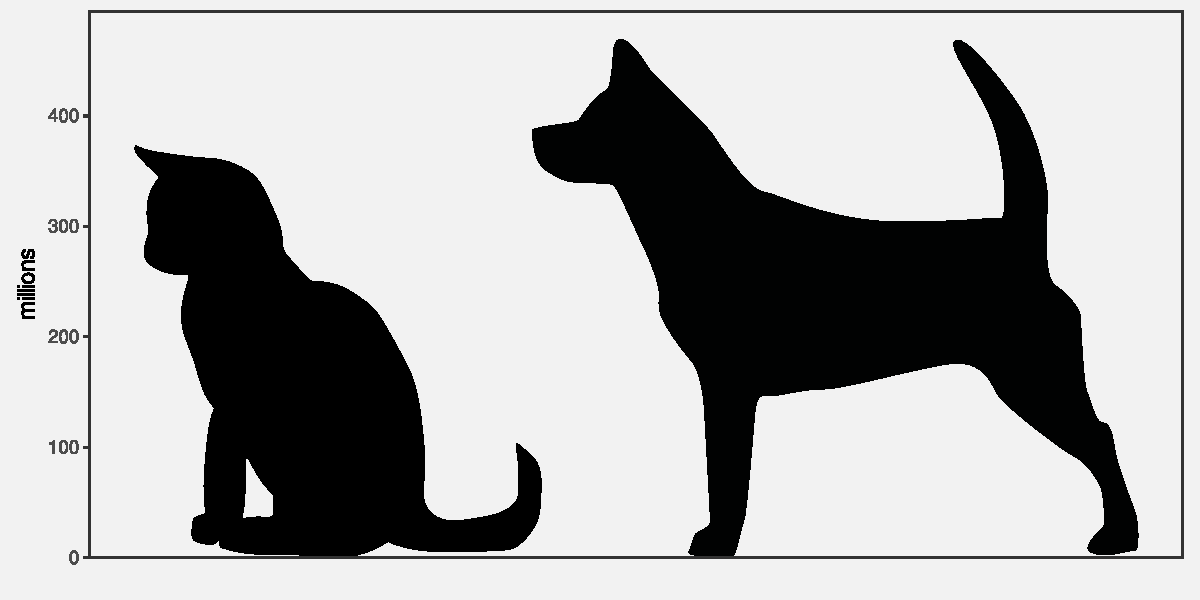
\includegraphics[width=1\linewidth,height=\textheight,keepaspectratio]{index_files/mediabag/visual-objects_files/figure-pdf/fig-pic-1.pdf}

}

\caption{\label{fig-pic}A data visualisation of the number of pet cats
and pet dogs worldwide.}

\end{figure}%

Figure~\ref{fig-pic-alt} shows two alternative uses of icons that
attempt to resolve some of the problems in Figure~\ref{fig-pic}. In
Figure~\ref{fig-pic-alt-1}, the images are distorted so that they have
the same width and so that only the height of the images changes. There
is also a bar to help with the perception of \textbf{length}. While the
bar makes it much easier to decode the number of pets, the distortion is
not effective because it hinders the perception of the icon.

Figure~\ref{fig-pic-alt-2} uses a bar to represent the number of pets
and just has a small version of the icon at the base of each bar. We
know that the bar is effective for decoding the number of pets and the
small icons are effective as labels for the bars.

\begin{figure}

\begin{minipage}{0.50\linewidth}

\centering{

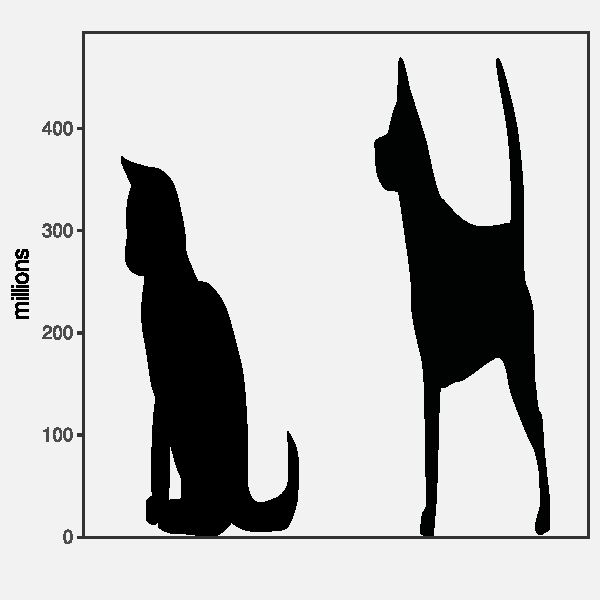
\includegraphics[width=1\linewidth,height=\textheight,keepaspectratio]{index_files/mediabag/visual-objects_files/figure-pdf/fig-pic-alt-1.pdf}

}

\subcaption{\label{fig-pic-alt-1}distorted icons}

\end{minipage}%
%
\begin{minipage}{0.50\linewidth}

\centering{

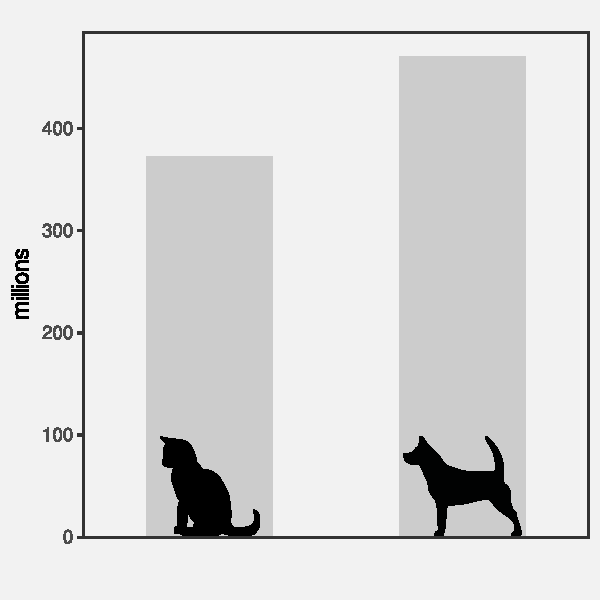
\includegraphics[width=1\linewidth,height=\textheight,keepaspectratio]{index_files/mediabag/visual-objects_files/figure-pdf/fig-pic-alt-2.pdf}

}

\subcaption{\label{fig-pic-alt-2}icon labels}

\end{minipage}%

\caption{\label{fig-pic-alt}Two alternative uses of icons.}

\end{figure}%

Figure~\ref{fig-pic-icon} shows two more alternatives to
Figure~\ref{fig-pic}. Figure~\ref{fig-pic-icon-2} is just a standard bar
plot. We know that this is effective for decoding the number of pets.

Figure~\ref{fig-pic-icon-1} uses repetitions of the icons to represent
the number of pets, still within a bar. In this case, each icon
represents 100 million pets. The ability to count icons is effective for
decoding the overall counts.\footnote{cite the study that reckons using
  icons can help with perceiving counts. More effective when each icon
  represents 1 (and so there are no fractional icons) ?}

\begin{figure}

\begin{minipage}{0.50\linewidth}

\centering{

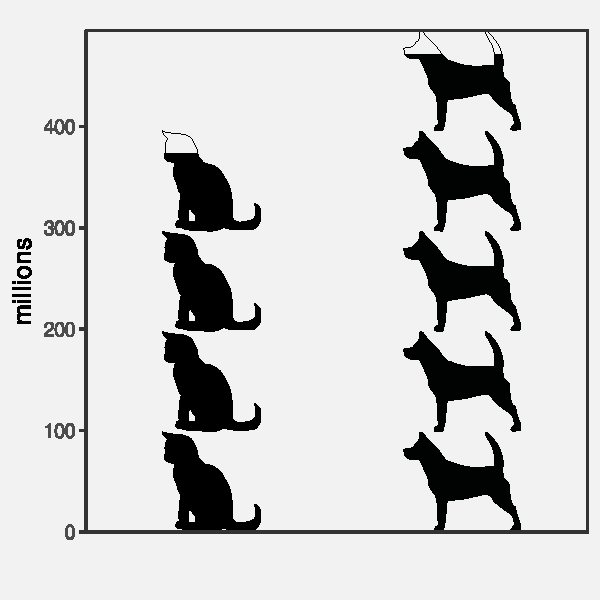
\includegraphics[width=1\linewidth,height=\textheight,keepaspectratio]{index_files/mediabag/visual-objects_files/figure-pdf/fig-pic-icon-1.pdf}

}

\subcaption{\label{fig-pic-icon-1}Icons are repeated to represent the
number of pets.}

\end{minipage}%
%
\begin{minipage}{0.50\linewidth}

\centering{

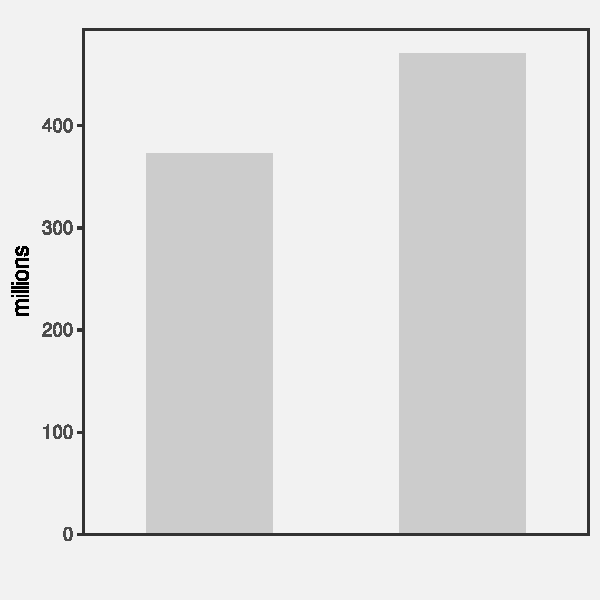
\includegraphics[width=1\linewidth,height=\textheight,keepaspectratio]{index_files/mediabag/visual-objects_files/figure-pdf/fig-pic-icon-2.pdf}

}

\subcaption{\label{fig-pic-icon-2}A basic bar plot}

\end{minipage}%

\caption{\label{fig-pic-icon}Two more alternative data visualisations of
the pet data.}

\end{figure}%

\section{Case study: Chernoff faces}\label{case-study-chernoff-faces}

Figure~\ref{fig-chernoff} visualises the 2023 Rugby World Cup data
(Table~\ref{tbl-rwc-2023}) using Chernoff faces.\footnote{Chernoff
  (1973)} The data symbol in this visualisation is a little unusual;
each country is represented by a combination of circles, curves, and
lines that together produce a \textbf{visual object} that resembles a
face. The mappings in this visualisation are also a little unusual. The
number of points scored is encoded as the \textbf{curvature} of the
smile, the number of tries is encoded as the \textbf{angle} of the eye
brows, and the number of clean breaks is encoded as the horizontal
\textbf{position} of the eyes.

\begin{verbatim}
Warning: The `scale_name` argument of `continuous_scale()` is deprecated as of ggplot2
3.5.0.
\end{verbatim}

\begin{figure}

\centering{

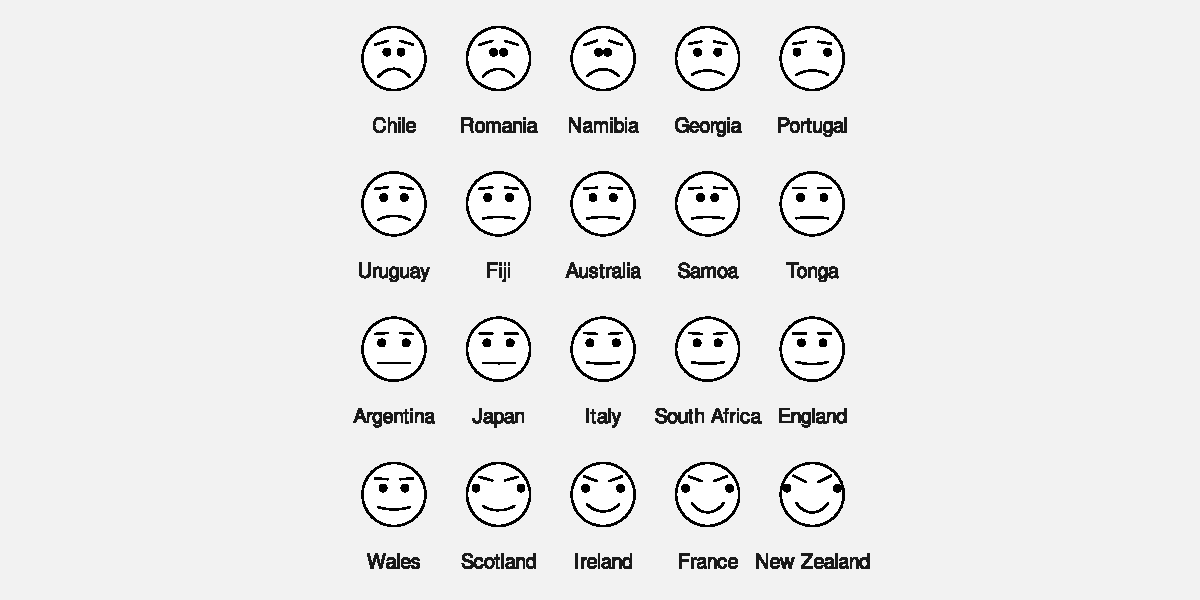
\includegraphics[width=1\linewidth,height=\textheight,keepaspectratio]{index_files/mediabag/visual-objects_files/figure-pdf/fig-chernoff-1.pdf}

}

\caption{\label{fig-chernoff}A Chernoff faces plot of the \ldots{}}

\end{figure}%

The mappings in a Chernoff face are \emph{not} very accurate (see
Section~\ref{sec-accuracy}; \textbf{curvature} is ranked \emph{below}
colour in terms of accuracy),\footnote{Link to a resource that has a
  comprehensive list of visual channels and includes curvature.} so
Cheroff faces are \emph{not} very effective for decoding raw data
values.

However, the familiarity of Chernoff faces means that we are easily able
to perceive common combinations of the facial features. For example, we
can see several sad, worried faces at the top-left of
Figure~\ref{fig-chernoff} and several happy, perhaps even smug, faces at
the bottom-right. We can perceive countries that share similar
combinations of performance measures. In other words, we can perceive
multi-dimensional correlations and multi-dimensional groupings in the
data.

In this case, the happier faces have been arranged to correspond to the
more successful teams and the teams have been ordered from least points
scored to most points scored. The resulting proximity helps with
perceiving groups of similar faces.

\begin{quote}
A Chernoff face is effective at conveying multi-dimensional
relationships because the data symbol is a familiar visual object from
which we can easily perceive simple human emotions.
\end{quote}

\section{Dangers of learned mappings}\label{sec-learned-danger}

Figure~\ref{fig-stroop} provides a demonstration of the Stroop
Effect.\footnote{citation please!} The task is to name the colour of
each word. This task is difficult to do because there are two decodings
involved and the two decodings are inconsistent. Each set of letters has
a learned decoding based on the \textbf{shape} of the letters---the word
that the letters spell out---but there is also a learned decoding based
on the actual \textbf{colour} of the letters---the colour names that we
learn as children.

\begin{figure}

\centering{


\includegraphics[width=1\linewidth,height=\textheight,keepaspectratio]{index_files/mediabag/visual-objects_files/figure-pdf/fig-stroop-1.pdf}

}

\caption{\label{fig-stroop}The Stroop effect. Try to name the
\emph{colour} of each word.}

\end{figure}%

One issue with relying on learned decodings is that we may learn more
than one association for the same visual feature. For example, the
colour red is commonly associated with hot (versus blue for cold), but
also with stop (versus green for go), plus also passion, or even
anger.\footnote{Cite ``Sometimes more is more: iterative participatory
  design of infographics for engagement of community members with
  varying levels of health literacy'' Arcia et al (2016) where people
  interpret icons in multiple ways, e.g., specifically ``pineapple''
  rather than generic ``fruit''. Also cite something about cultural
  differences in perception. e.g., ``More of what? Dissociating effects
  of conceptual and numeric mappings on interpreting colormap data
  visualizations'' Soto et al (2023)} Furthermore, many associations are
specific to a particular culture. For example, red is associated with
luck and prosperity in Chinese culture, among other things.\footnote{``A
  Study on the Metaphor of ``Red'' in Chinese Culture'' Qiang (2011)}

Relying on a learned decoding can cause confusion if there are multiple
possible decodings. It may not be clear which data value should be
decoded from the visual feature (Figure~\ref{fig-ambiguous-decode}).

\begin{figure}

\centering{

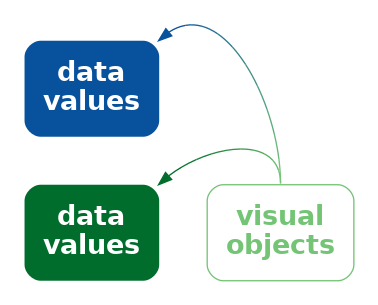
\includegraphics[scale=0.5]{Diagrams/ambiguous-decode.png}

}

\caption{\label{fig-ambiguous-decode}A visual feature may have more than
one learned decoding, which means that we may decode more than one value
from the visual feature.}

\end{figure}%

The problem is much worse if the learned decoding(s) conflict with an
explicit encoding of data values. For example, in
Figure~\ref{fig-flags}, if we use the incorrect flag for a country, for
example, by swapping the Australian and New Zealand flags, we not only
introduce confusion, but a misleading decoding. This is similar to the
problem of dissonant mappings (Section~\ref{sec-dissonance} and
Figure~\ref{fig-dissonant-decode}).

Suppose that we made a similar change to
Figure~\ref{fig-scatter-country}, swapping the open triangle for
Australia and the square-with-a-plus symbol for New Zealand. That would
not cause any problem because there is no learned decoding to conflict
with. We only get the problem if we swap flags in Figure~\ref{fig-flags}
because of the conflict with learned decodings.

\begin{quote}
Employing a learned decoding incorrectly can at best weaken and at worst
destroy the effectiveness of a data visualisation.
\end{quote}

\section{The dangers of visual
objects}\label{the-dangers-of-visual-objects}

One issue with more complex data visualisations is that their
effectiveness depends on a larger amount of learning and experience. If
the viewer does not have the knowledge required to decode a visual
object, then the data visualisation will fail. We saw an example of this
in Figure~\ref{fig-flags-direct}, where the familiarity of different
country flags will vary with nationality and age, for example.

An extreme version of this problem is the use of not just complex or
unusual data symbols, but entirely novel data visualisations.\footnote{Kosslyn's
  Principle of appropriate knowledge ?}

Andrews curve of RWCperGame statistics (analogue of
Figure~\ref{fig-parallel}). \textbf{Cite Andrews article.} Can see the
three distinct groups of countries more easily in this than in parallel
plot, but hard to understand exactly what you are seeing. Plus NO chance
of recovering original data values (another example of visualising data
summary).

\begin{figure}

\centering{

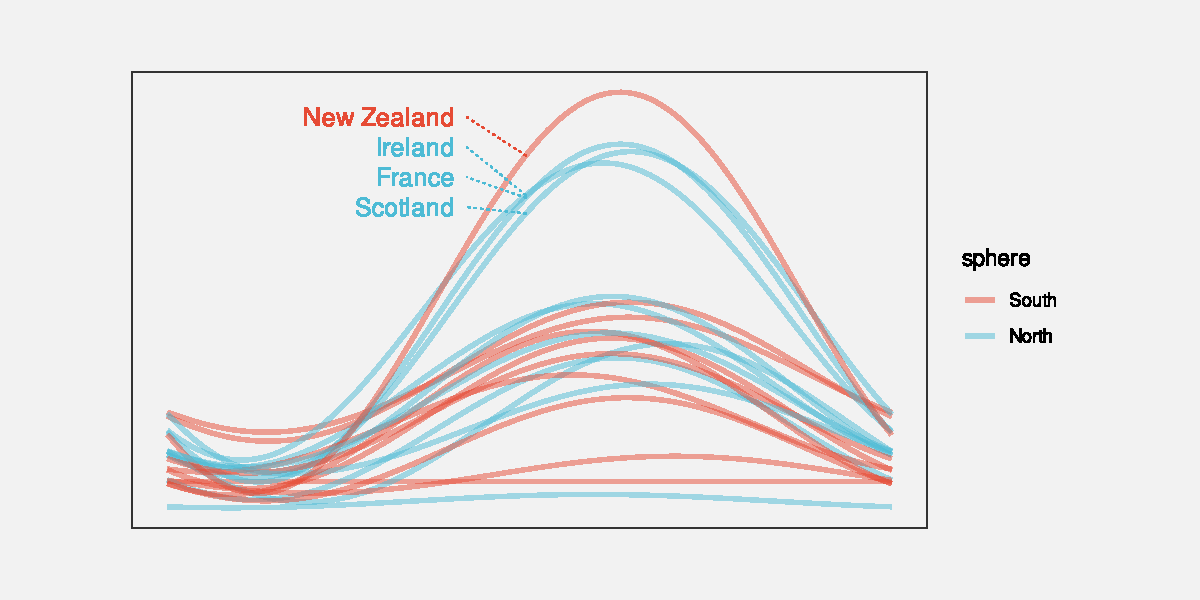
\includegraphics[width=1\linewidth,height=\textheight,keepaspectratio]{index_files/mediabag/visual-objects_files/figure-pdf/fig-andrews-1.pdf}

}

\caption{\label{fig-andrews}An Andrews plot of the performance measures
for teams in the 2023 Rugby World Cup.}

\end{figure}%

Another example of this problem are the hurrican ``cones of
uncertainty'' that Cairo highlights in Chapter 5 of How Charts Lie
(footnote!).

Mention that little is known about the accuracy of visual objects
(though they must have good capacity because they are more abstract,
right?)\footnote{in general, there needs to be more explicit
  acknowledgement of the lack of experimental results for complex data
  vis scenarios. c.f., ``Testing Statistical Charts: What Makes a Good
  Graph?'' Vanderplas, Cook, and Hofmann (2020) p 71.}:

\section{Summary}\label{summary-11}

If we encode data values as familiar visual objects, it becomes possible
to decode more complex concepts based on prior learning and experience.

This may obviate the need for legends.

\begin{center}\rule{0.5\linewidth}{0.5pt}\end{center}

\theendnotes

\bookmarksetup{startatroot}

\chapter{Text}\label{text}

Figure~\ref{fig-no-text} is a version of Figure~\ref{fig-crime} with all
of the text removed. Although we can see that some values, or rather
three sets of values, haved decreased, we cannot tell what the values
are or by how much they have decreased. If there was ever any doubt,
Figure~\ref{fig-no-text} makes it clear that text is doing a lot of
important work in a data visualisation.

\begin{figure}

\centering{

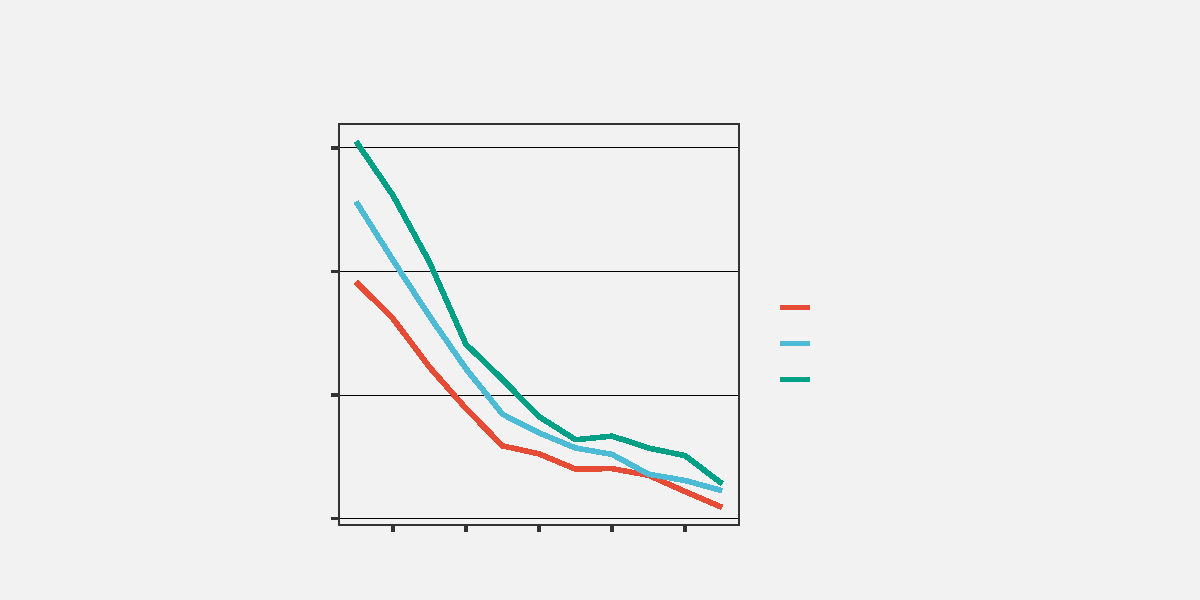
\includegraphics[width=1\linewidth,height=\textheight,keepaspectratio]{index_files/mediabag/text_files/figure-pdf/fig-no-text-1.pdf}

}

\caption{\label{fig-no-text}A line plot with all text removed. Without
text, it is impossible to know what data values are represented in this
plot.}

\end{figure}%

Eye-tracking studies also show that people spend a lot of time looking
at the text within a data visualisation. For example, in
Figure~\ref{fig-fixations-text}, there are more fixations in the regions
that contain text than anywhere else. There is also evidence that text
elements are more memorable than the other elements of a data
visualisation.\footnote{``a memorable visualization is often also an
  effective one.'' (``Beyond Memorability: Visualization Recognition and
  Recall'' Borkin et al (2016)) Only a thumbnail version of the original
  image is shown in Figure~\ref{fig-fixations-text} in order to comply
  with terms of use of the MASSVIS data set.}

\begin{figure}

\begin{minipage}{0.50\linewidth}

\pandocbounded{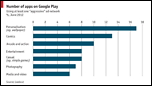
\includegraphics[keepaspectratio]{MASSVIS/economist_daily_chart_75-thumb.png}}

\subcaption{\label{fig-fixations-text-1}A thumbnail of the original data
visualisation.}

\end{minipage}%
%
\begin{minipage}{0.50\linewidth}

\pandocbounded{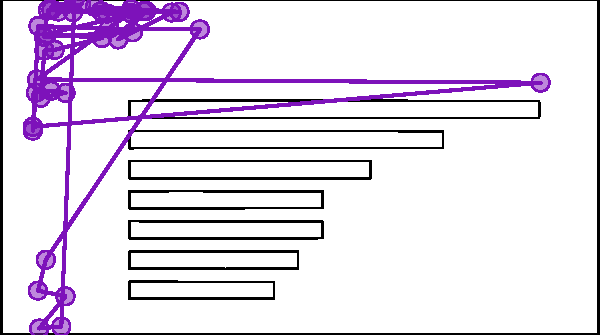
\includegraphics[keepaspectratio]{index_files/mediabag/MASSVIS/economist_daily_chart_75-track.pdf}}

\subcaption{\label{fig-fixations-text-2}Fixations and saccades from eye
tracking data.}

\end{minipage}%

\caption{\label{fig-fixations-text}Eye tracking data from the MASSVIS
project that shows fixations (circles) and saccades (lines between
circles) for one person viewing an image for 10 seconds.}

\end{figure}%

This section looks at the role that text plays in making data
visualisations work.\footnote{Provide citation to Brath book at least.
  Perhaps cite my text article, however that gets to see the light of
  day.}

\section{Data symbols}\label{sec-data-symbols}

Figure~\ref{fig-bar-text} is a version of Figure~\ref{fig-bar} with
white text added to each bar showing the exact number of offenders in
each ethnic group. This is an example of using text as a \textbf{data
symbol}.

\begin{figure}

\centering{

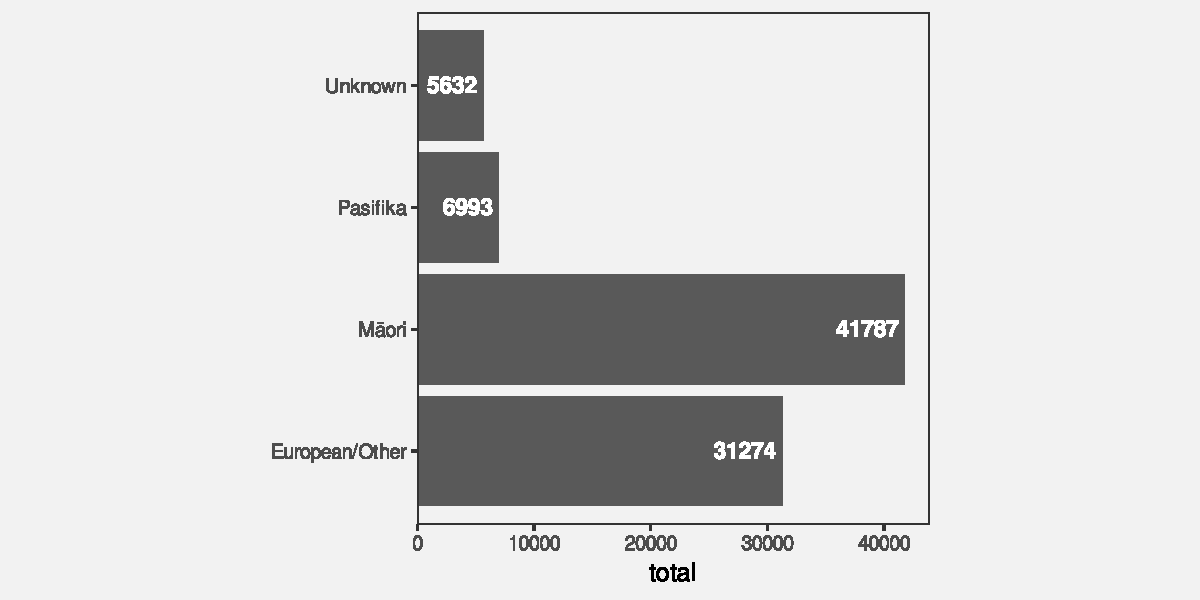
\includegraphics[width=1\linewidth,height=\textheight,keepaspectratio]{index_files/mediabag/text_files/figure-pdf/fig-bar-text-1.pdf}

}

\caption{\label{fig-bar-text}A bar plot of the total number of offenders
for different ethnic groups. The data symbols in this plot are the
horizontal bars \emph{and} the text values at the end of each bar.}

\end{figure}%

Just as data values are mapped to the visual features of the bar data
symbols in Figure~\ref{fig-bar-text}, data values are also mapped to the
visual features of the text data symbols. For example, the ethnic groups
are encoded as the vertical \textbf{position} of the bars \emph{and} as
the vertical \textbf{position} of the text. The data values for the
number of offenders in each ethnic group are encoded as the
\textbf{length} of the bars \emph{and} as the horizontal
\textbf{position} of the text. Furthermore, the data values for the
number of offenders in each ethnic group are encoded as the
\textbf{shape} of the text---the letters and digits that make up the
text.

Just as we can decode data values from the visual features of the bars
in Figure~\ref{fig-bar-text}, we can decode data values from the visual
features of the text. For example, we can see just from the horizontal
position of the text, without reading the text values, that some counts
are (much) larger than others.

\begin{quote}
Encoding data values as the position, colour, and size of text data
symbols is effective for the same reasons that these visual features are
effective for other types of data symbols.
\end{quote}

We see examples of the use of simple visual features in text in almost
any piece of writing. For example, section headings are typically larger
and bolder than the main text in a report and the
\href{exec.html}{Executive Summary} in this book makes use of colour and
angle to create visual connections between associated terms within a
bullet-point list.

However, the unique power of text comes from \textbf{decoding} the
\textbf{shape} of the text. Text is the ultimate example of a
\textbf{learned mapping} (Section~\ref{sec-learned}). We all learn to
read text (and numbers), which means that, when we are presented with a
text shape, there is a pre-existing decoding to the semantic content of
the text (Figure~\ref{fig-learned-decode}). For example, in
Figure~\ref{fig-bar-text}, we are able to decode the data value
\texttt{41787} (the count for Māori) from the text ``41787''.
Furthermore, this decoding is extremely accurate and very flexible.

Figure~\ref{fig-scatter-text} shows another example of text data symbols

\begin{figure}

\centering{

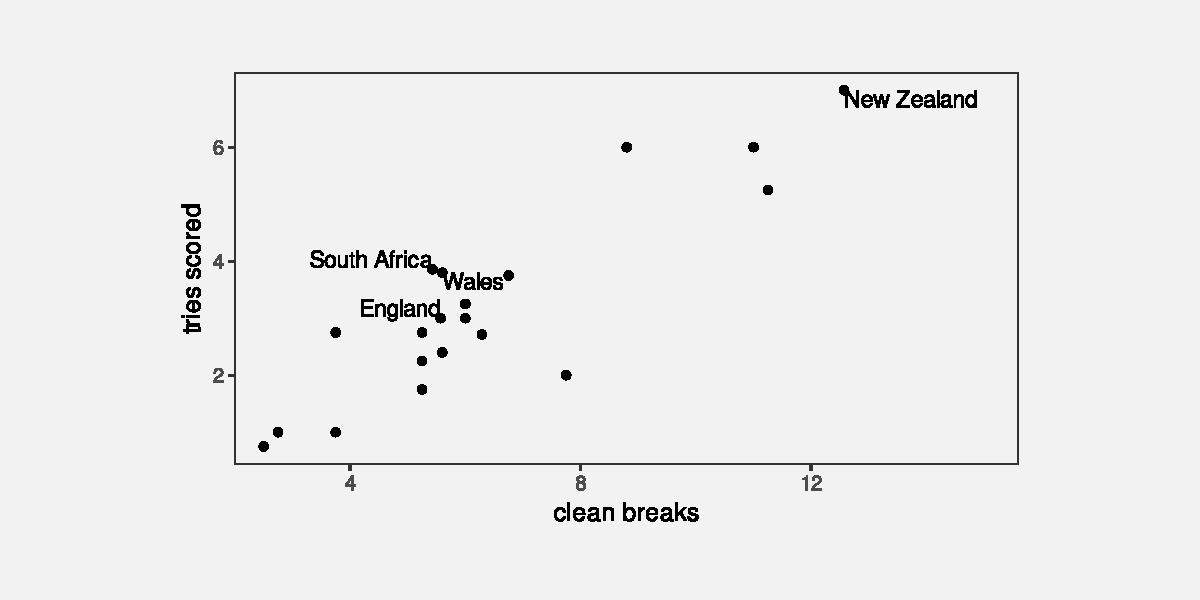
\includegraphics[width=1\linewidth,height=\textheight,keepaspectratio]{index_files/mediabag/text_files/figure-pdf/fig-scatter-text-1.pdf}

}

\caption{\label{fig-scatter-text}A scatter plot of the number of times a
team breaks through the opposition defence and the number of tries that
a team scores (both are per-game averages) for teams at the 2023 Rugby
World Cup.}

\end{figure}%

In terms of the criteria that we discussed in
Chapter~\ref{sec-mapping-visual-features}, the value of text data
symbols is that they allow us to decode data values very
\textbf{accurately} (Figure~\ref{fig-decode}). Text is also very
flexible because it is appropriate for both \textbf{quantitative} and
\textbf{qualitative} data values. Finally, text has a very large
\textbf{capacity}; we are able to distinguish between many different
words and numbers.

\begin{quote}
Text data symbols are effective because they can be used to represent
any sort of data and they allow a very accurate decoding of data values.
\end{quote}

Compared to the bar data symbols in Figure~\ref{fig-bar-text}, the text
data symbols are much more complex shapes. In terms of the simple visual
processing model from Section~\ref{sec-visual-processing}, the text data
symbols are similar to \textbf{visual objects}. This means that text can
convey more sophisticated information, at the expense of more cognitive
effort, and with a limit on how many shapes we can process
simultaneously (see Figure~\ref{fig-visual-model}).\footnote{Talk about
  there being separate verbal processing areas in the brain. Text has to
  come in as visual, so undergoes visual processing, but text is also
  processed separately for its language value. Cite Ware p315-316}

One weakness of text data symbols is that comparing values (rather than
just decoding a single value) requires more cognitive effort compared to
comparing simple visual features (like the lengths of bars). For
example, in Figure~\ref{fig-bar}, it is quick and easy to approximate
the ratio of Pasifika to Māori or European/Other to Māori from the
lengths of the bars, but those comparisons are slower and take more
conscious effort using the text data symbols in
Figure~\ref{fig-bar-text}.

\begin{quote}
It is harder to compare data values that are mapped to text because it
requires more effort to decode data values and to perform mental
calculations.
\end{quote}

In addition, our visual system cannot generate \textbf{visual summaries}
of large amounts of text (Section~\ref{sec-visual-summaries}). This is
why a table of numbers, like Table~\ref{tbl-crime}, is ineffective for
perceiving groups of values or trends in values.

\begin{quote}
Large numbers of text data symbols are \emph{not} effective because the
visual system cannot decode visual summaries from the text.
\end{quote}

Why si a picture is worth a thousand words? Because 1000 words is 1000
fixations, identifying 1000 visual objects, and then interpreting their
combined meaning.

\section{Guides}\label{sec-guides}

Figure~\ref{fig-crime-guides} is a version of Figure~\ref{fig-crime}
with the guides highlighted in purple. There are tick marks and tick
labels on the x-axis and y-axis, there are horizontal grid lines, and
there are legend elements to show the mapping from the different ages to
different colours.

\begin{figure}

\centering{

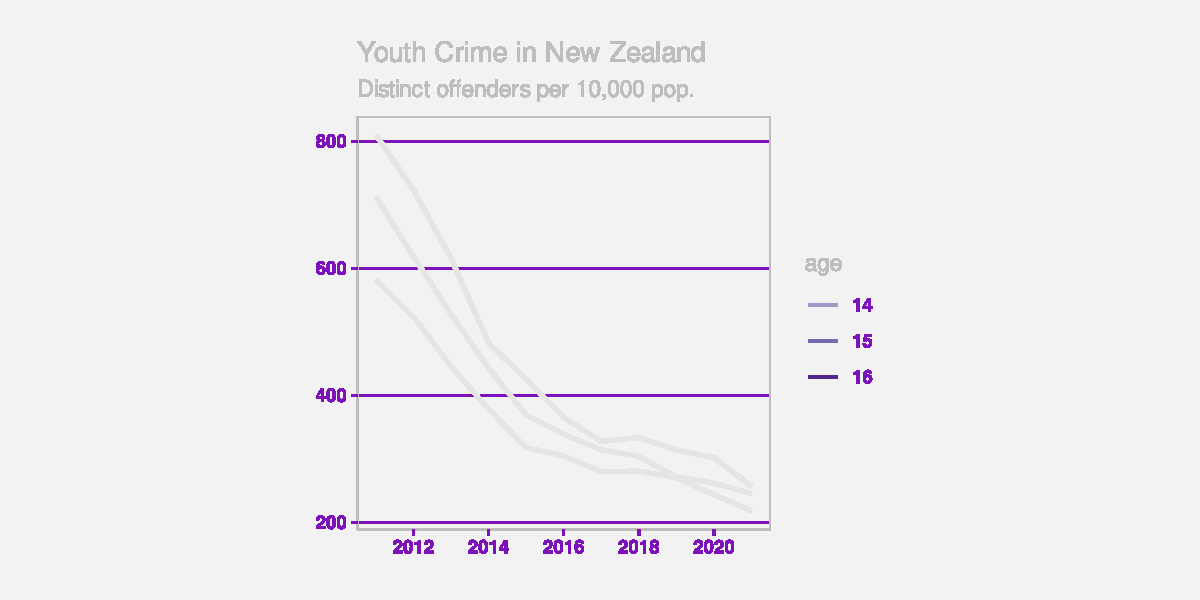
\includegraphics[width=1\linewidth,height=\textheight,keepaspectratio]{index_files/mediabag/text_files/figure-pdf/fig-crime-guides-1.pdf}

}

\caption{\label{fig-crime-guides}A line plot of the crime rate amongst
youth offenders aged 14 to 16 from 2011 to 2021. The guides in this plot
have been highlighted in purple.}

\end{figure}%

The first thing to note about the guides in
Figure~\ref{fig-crime-guides} is that they are all composed of
\textbf{data symbols}, with \textbf{data values} mapped to
\textbf{visual features} of the data symbols
(Chapter~\ref{sec-mapping-visual-features}). This is perhaps easiest to
see with the grid lines. Each grid line is a data symbol where a data
value, a rate of offending, has been encoded as the vertical
\textbf{position} of the line. Similarly, each tick mark on the y-axis
is a line data symbol where a rate of offending has been encoded as the
vertical \textbf{position} of the line and each tick mark on the x-axis
is a line data symbol where a year has been encoded as the horizontal
\textbf{position} of the line. Finally, each of the tick labels on the
y-axis is a text data symbol where a rate of offending has been encoded
as the vertical \textbf{position} of the text \emph{and} as the
\textbf{shape} of the text. Similar mappings apply to the x-axis tick
labels. The legend is also made up of line data symbols and text data
symbols, this time with age data values encoded as the \textbf{colour}
of lines and the \textbf{shape} of text.

The \textbf{decoding} of the \textbf{shape} of the \textbf{text} data
symbols within the guides shows the critical role that text plays within
guides. If we look again at Figure~\ref{fig-no-text}, there are coloured
lines on the plot and there are coloured lines on the legend. The fact
that these lines have different colours indicates that there are three
different groups, but the colours alone do not tell us what the groups
are. We can decode different values from the colours of the lines, but
we cannot decode exact data values. In the original
Figure~\ref{fig-crime}, the shapes of the text labels on the legend
allow us to decode the original data values---the three ages 14, 15, and
16.

The proximity of the text labels in the legend to the coloured lines in
the legend means that we associate each label with each coloured line
(Section~\ref{sec-visual-model-groups}). So the text labels in the
legend are the essential data symbols in Figure~\ref{fig-crime} because
only they allow us to decode from the colours of the lines to the three
age groups.

The text labels on axes perform a similar service. For example, the
numbers on the axes in Figure~\ref{fig-crime} are the only data symbols
that provide exact decoding from positions to data values (years or
rates). The lines within the plot, by themselves, only show that values
are decreasing. It is only the relative position of the lines within the
plot to the tick labels on the axes (and the grid lines) that allows us
to decode from the lines within the plot to (approximate) data values.

Text data symbols within guides are effective because guides contain
only a few data values that need to be decoded precisely. This is the
situation where text excels.

\begin{quote}
Guides are effective because they encode known data values as text data
symbols as well as the data symbols used in the main plot.
\end{quote}

\section{Labels}\label{sec-labels}

Figure~\ref{fig-crime-labels} shows a version of Figure~\ref{fig-crime}
with the labels highlighted in purple. In this data visualisation, the
only labels are the overall plot title and the legend title. It is also
common to see axis titles.

\begin{figure}

\centering{

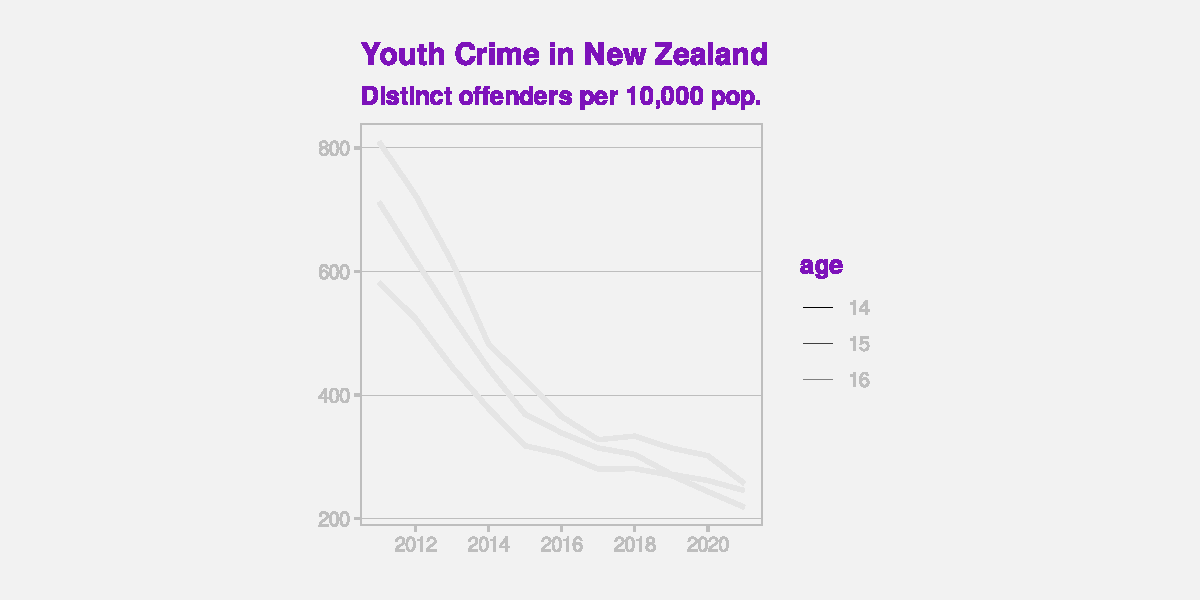
\includegraphics[width=1\linewidth,height=\textheight,keepaspectratio]{index_files/mediabag/text_files/figure-pdf/fig-crime-labels-1.pdf}

}

\caption{\label{fig-crime-labels}A line plot of the crime rate amongst
youth offenders aged 14 to 16 from 2011 to 2021. The labels in this plot
have been highlighted in purple.}

\end{figure}%

The difference between labels and the other components of a data
visualisation, the data symbols and the guides, is that labels relate to
\textbf{metadata} rather than raw data values. We can still consider
this a mapping, just one that involves encoding metadata rather than
data values (Figure~\ref{fig-label-mapping}).

\begin{figure}

\centering{

\begin{figure}[H]

\begin{minipage}{0.50\linewidth}
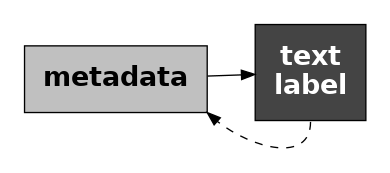
\includegraphics[scale=0.5]{Diagrams/meta-label.png}\end{minipage}%

\end{figure}%

}

\caption{\label{fig-label-mapping}Labels can be viewed as an encoding of
metadata as text. We can encode complex information using text and we
can decode text with extremely high fidelity.}

\end{figure}%

Labels contain information like descriptions of variables and units of
measurement and references to data sources. These are all important
pieces of information, but they are more complex, more abstract, and far
fewer in number than data values. Fortunately, text is very capable of
expressing complex information and works very well in small amounts, so
it is ideal for this role.

To emphasise that point, imagine how impossible it would be to encode
the information in the title of Figure~\ref{fig-crime-labels}, or just
the legend title, only using simple geometric data symbols like bars and
points. Using pictograms, which have learned decodings like text, would
also be very difficult because it is much harder to compose pictograms
in the way that text can be composed into phrases and sentences.

\begin{quote}
Text is the only way to encode the type of complex and abstract
information that is required for titles and axis labels.
\end{quote}

Another use of text in a data visualisation is to label specific points
of interest. For example, Figure~\ref{fig-ann} shows a variation of
Figure~\ref{fig-scatter}, with text added to help explain the result of
the Rugby World Cup final to disillusioned New Zealanders. This
demonstrates further the value of text as the only way to encode complex
and nuanced information.\footnote{Russell Ackoff's ``From Data to
  Wisdom'' Text is very flexible - it can convey data, information,
  knowledge, understanding, and wisdom. Most other graphical elements
  are much more limited.}

\begin{figure}

\centering{

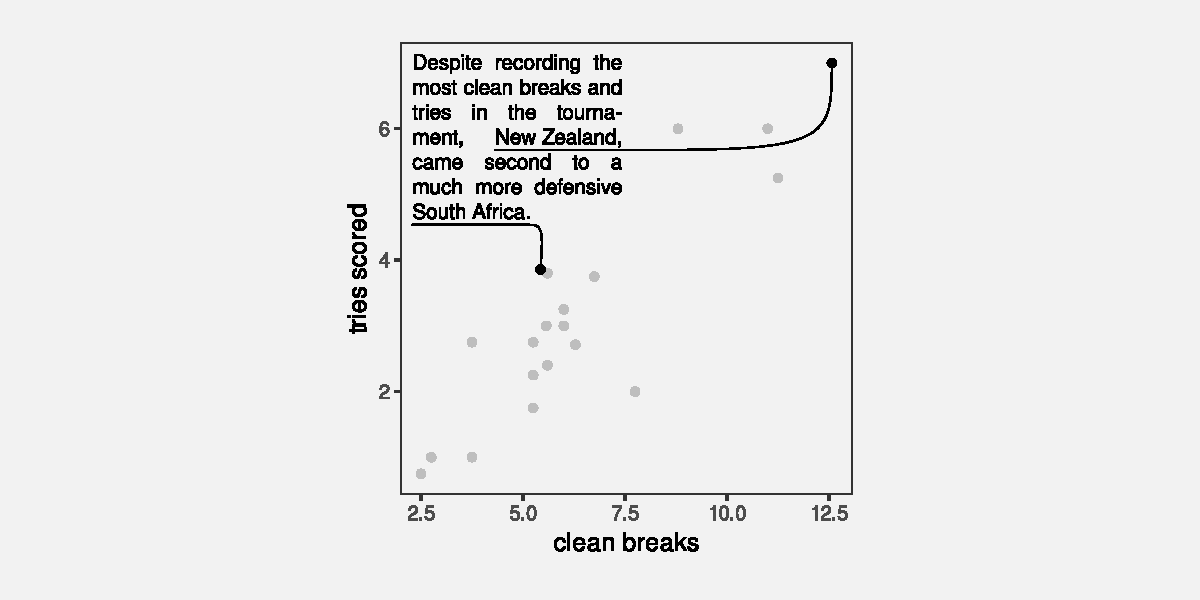
\includegraphics[width=1\linewidth,height=\textheight,keepaspectratio]{index_files/mediabag/text_files/figure-pdf/fig-ann-1.pdf}

}

\caption{\label{fig-ann}The number of times a team breaks through the
opposition defence and the number of tries that a team scores (both are
per-game averages) for teams in the 2023 Rugby World Cup.}

\end{figure}%

Figure~\ref{fig-ann} also demonstrates that text is an effective way of
directing attention (Section~\ref{sec-attention}).\\
Text labels can explicitly describe data values or, more usefully, data
summaries that the data visualisation is designed to show.\footnote{Mention
  idea of top-down as opposed to bottom-up attention. With cite.}

\section{Case study: Word clouds}\label{sec-word-cloud}

Figure~\ref{fig-wordcloud} shows a word cloud data visualisation based
on the text of the Wikipedia page on the Rugby World Cup.\footnote{\href{https://en.wikipedia.org/wiki/Rugby_World_Cup}{}
  (Wikipedia 2024)} This visualisation shows the frequency with which
different words appear on the Wikipedia page. The data values that are
being visualised are shown in Table~\ref{tbl-wiki-rwc}.

\begin{figure}

\centering{

\pandocbounded{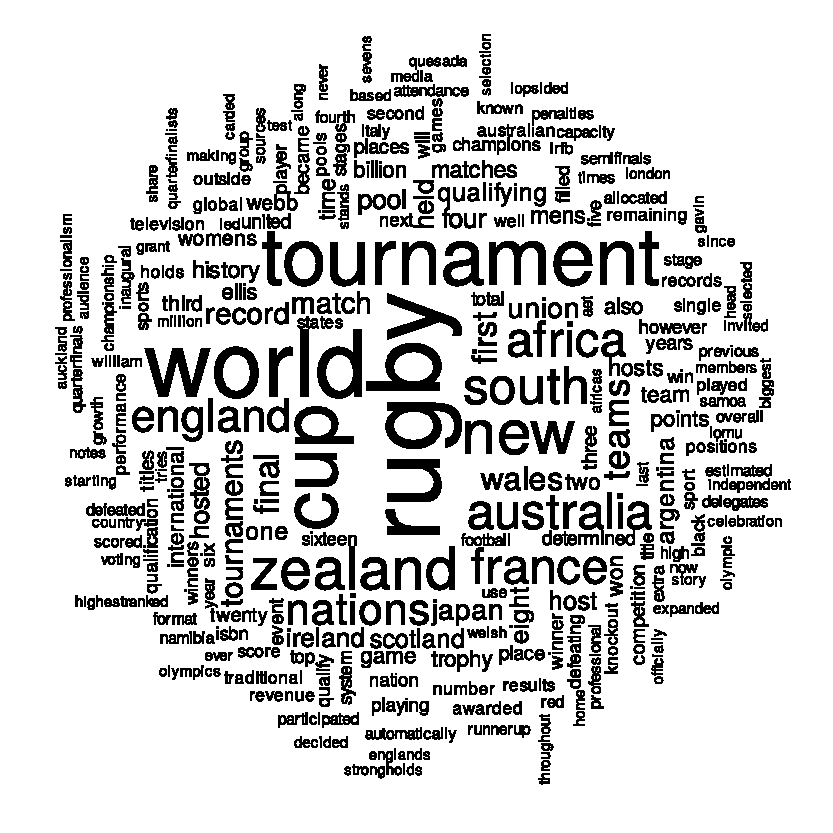
\includegraphics[keepaspectratio]{index_files/mediabag/Data/RWC/WordCloud/wordcloud-trim.pdf}}

}

\caption{\label{fig-wordcloud}A word cloud of the frequency of words in
the Wikipedia page for the Rugby World Cup.}

\end{figure}%

This data visualisation is unusual because it consists entirely of text
\textbf{data symbols}. The mappings in Figure~\ref{fig-wordcloud}
include encoding each word as the \textbf{shape} of a text data symbol
and encoding frequency as the \textbf{size} of a text data symbol. There
is no need for a guide for the mapping from words to text shape because
there is a learned decoding (Figure~\ref{fig-learned-decode}); we can
decode each text data symbol into a word data value because that
decoding has already been learned.

There is no guide for the mapping from word frequency to text size, so
we cannot decode exact word frequencies. Table~\ref{tbl-wiki-rwc} shows
the six most frequent words. However, the visualisation is still
effective at conveying the \emph{relative} frequencies. The larger words
occurred more frequently. For example, we can see the names of the teams
that were most successful at the tournament, like New Zealand and South
Africa, are much larger than less successful teams.

\begin{longtable}[]{@{}lr@{}}

\caption{\label{tbl-wiki-rwc}A table of the number of times different
words occur in the Wikipedia page for the Rugby World Cup (for words
that appear more than once). There are 287 different words, but only the
first 6 are shown here.}

\tabularnewline

\toprule\noalign{}
word & freq \\
\midrule\noalign{}
\endhead
\bottomrule\noalign{}
\endlastfoot
rugby & 72 \\
world & 66 \\
tournament & 56 \\
cup & 54 \\
new & 41 \\
zealand & 38 \\

\end{longtable}

The encoding of frequencies as the \textbf{size} of the words does not
provide the best \textbf{accuracy} for decoding frequencies
(Section~\ref{sec-accuracy}) and this made worse by the fact that longer
words become even larger. This means that we cannot identify the exact
frequency of any one word, we cannot identify the quantitative
difference in frequency between pairs of words, and we cannot easily
perceive the distribution of frequencies across words. A word cloud is
only effective for approximate ordinal comparisons of word frequencies
(Chapter~\ref{sec-mapping-visual-features}).

Frequency is also mapped to \textbf{position in space}, with more
frequent words placed towards the centre of the word cloud. This is an
example of redundant mapping; more frequent words are both larger
\emph{and} more central (Section~\ref{sec-redundant}).

\begin{quote}
A word cloud is effective for conveying words because it maps words to
text data symbols. It is also partially effective for conveying relative
frequencies of words because it maps word frequency to both size and
position in space.
\end{quote}

Another benefit of encoding frequency as position in space is the
efficient use of space. For example, Figure~\ref{fig-wordcloud-bar}
shows the same data presented as a bar plot with the frequency of each
word mapped to a separate bar. Although the accuracy is improved for
comparing frequencies, the bar plot does not have as much room for the
words themselves.

\begin{figure}

\centering{

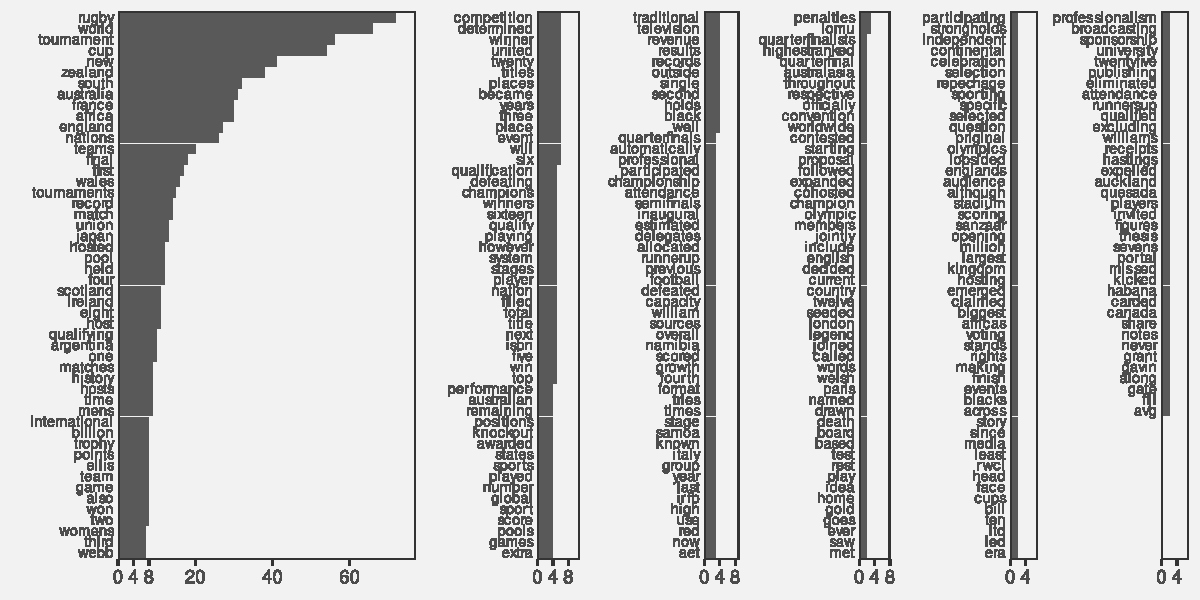
\includegraphics[width=1\linewidth,height=\textheight,keepaspectratio]{index_files/mediabag/text_files/figure-pdf/fig-wordcloud-bar-1.pdf}

}

\caption{\label{fig-wordcloud-bar}A bar plot of the frequency of
different words in the Wikipedia page for the Rugby World Cup.}

\end{figure}%

One weakness of the word cloud is that the \textbf{angle} of words
changes with no corresponding change in the data values. This is an
example of a \textbf{dissonant} mapping, which can cause confusion
(Section~\ref{sec-dissonance}). The viewer will notice the differences
in angle and attempt to decode that difference to a difference in data
values that does not exist.

\begin{quote}
The different angles of text in a word cloud is not effective because it
does not encode any differences in the data.
\end{quote}

\section{Case study: Tables}\label{case-study-tables}

Table~\ref{tbl-rwc-table} shows a subset of the 2023 Rugby World Cup
data set (Table~\ref{tbl-rwc-2023}), just including the top eight
nations in the tournament. We established in
Section~\ref{sec-data-symbols} that visualising data values in a table
provides an excellent basis for accurately decoding individual data
values, but imposes a larger cognitive burden for comparing values, and
is a very poor for extracting visual summaries, such as trends.

For example, it is very difficult to determine from
Table~\ref{tbl-rwc-table} whether there is any relationship between the
values in the four numeric columns.

\begin{longtable}[]{@{}llllll@{}}

\caption{\label{tbl-rwc-table}Performance measures for the top 8 teams
at the 2023 Rugby World Cup. Each measure is a per-game average because
some teams played more games than others.}

\tabularnewline

\toprule\noalign{}
country & sphere & runs & breaks & tries & points \\
\midrule\noalign{}
\endhead
\bottomrule\noalign{}
\endlastfoot
South Africa & South & 95.14 & 5.429 & 3.857 & 29.71 \\
England & North & 100.3 & 5.571 & 3 & 31.57 \\
Fiji & South & 138 & 5.6 & 2.4 & 22.4 \\
Wales & North & 109.4 & 5.6 & 3.8 & 32 \\
Argentina & South & 131.3 & 6.286 & 2.714 & 26.43 \\
Ireland & North & 137.6 & 8.8 & 6 & 42.8 \\
France & North & 126 & 11 & 6 & 47.6 \\
New Zealand & South & 139.3 & 12.57 & 7 & 48 \\

\end{longtable}

However, there are standard guidelines for formatting tables of values
that can improve the readability of a table.\footnote{For example,
  Schwabish (2020).

  Ehrenberg (1977) advice on tables

  ``UNDERSTANDING GRAPHS AND TABLES'' Wainer (1992)}
Table~\ref{tbl-rwc-table-tidy} shows the same data as
Table~\ref{tbl-rwc-table}, but with all of the numeric columns
right-aligned, a consistent number of decimal places in each column,
fewer decimal places than the data actually possess, and the rows have
been ordered from the highest number of points per game to the lowest.

It is easier to see some structure in Table~\ref{tbl-rwc-table}. For
example, the number of tries appears to decrease as well as the number
of points. We can also see some evidence of the number of breaks
decreasing as well, though it is weaker.

There are some familiar explanations for the improvement in the table
display. The reduction in detail, with fewer decimal places, means that
there is less complexity in the visual field. The consistent number of
decimal places means that less is changing, so differences are easier to
detect (Section~\ref{sec-differences}). Also, the consistent baseline
provided by right-alignment means that the text \textbf{length} of the
numbers (the number of digits in each number) provides a crude encoding
of the size of the number, particularly in the column showing the number
of clean breaks. However, it is worth noting that some of the
\textbf{accuracy} of the text has been sacrificed in order to make some
of these gains.

\begin{longtable}[]{@{}llrrrr@{}}

\caption{\label{tbl-rwc-table-tidy}Performance measures for the top 8
teams at the 2023 Rugby World Cup. This is a version of
Table~\ref{tbl-rwc-table} with some standard table design guidelines
applied.}

\tabularnewline

\toprule\noalign{}
country & sphere & runs & breaks & tries & points \\
\midrule\noalign{}
\endhead
\bottomrule\noalign{}
\endlastfoot
New Zealand & South & 139 & 12.6 & 7.0 & 48.0 \\
France & North & 126 & 11.0 & 6.0 & 47.6 \\
Ireland & North & 138 & 8.8 & 6.0 & 42.8 \\
Wales & North & 109 & 5.6 & 3.8 & 32.0 \\
England & North & 100 & 5.6 & 3.0 & 31.6 \\
South Africa & South & 95 & 5.4 & 3.9 & 29.7 \\
Argentina & South & 131 & 6.3 & 2.7 & 26.4 \\
Fiji & South & 138 & 5.6 & 2.4 & 22.4 \\

\end{longtable}

For comparison, Figure~\ref{fig-rwc-table} shows a scatter plot of the
data from Table~\ref{tbl-rwc-table}. The data symbol is a circle, with
the number of tries mapped to horizontal \textbf{position}, the number
of points mapped to vertical \textbf{position}, the number of clean
breaks mapped to \textbf{size}, and the number of runs mapped to
\textbf{colour} (shade). The relationships between tries and points and
between breaks and both tries and points are still easier to perceive in
this plot than in Table~\ref{tbl-rwc-table-tidy}, but
Table~\ref{tbl-rwc-table-tidy}, even with its rounding, still provides
better accuracy, particularly for breaks and runs.

\begin{figure}

\centering{

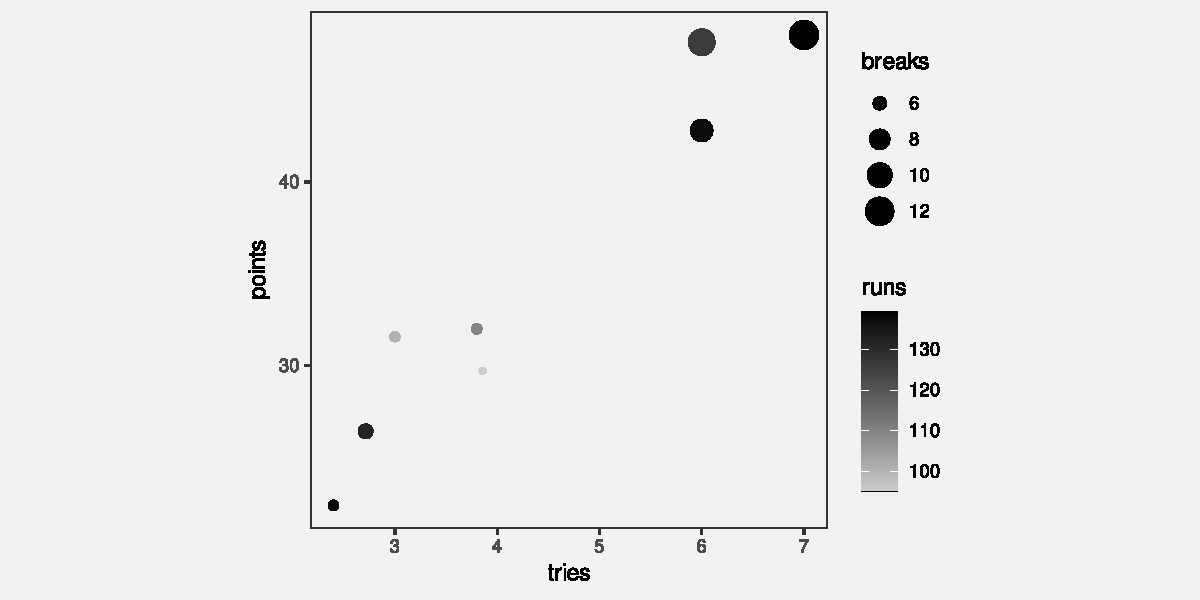
\includegraphics[width=1\linewidth,height=\textheight,keepaspectratio]{index_files/mediabag/text_files/figure-pdf/fig-rwc-table-1.pdf}

}

\caption{\label{fig-rwc-table}A scatter plot of the performance measures
for the top 8 teams at the 2023 Rugby World Cup.}

\end{figure}%

\section{Case study: Stem-and-leaf
plots}\label{case-study-stem-and-leaf-plots}

Figure Figure~\ref{fig-tries-hist} shows a histogram of the number of
tries scored by teams in the 2023 Rugby World Cup. The data symbols in
Figure~\ref{fig-tries-hist} are bars. The raw data values are the
average number of tries per game for each team, but the lengths of the
bars encode \textbf{data summaries}: the number of teams with an average
number of tries within each range: 0 to 1, 1 to 2, and so on.

Because the borders of the bars are not drawn, we get an emergent shape
from the combined bars (similar to a density plot;
Section~\ref{sec-density}).

This histogram allows us to see features of the data summaries, such as
a suggestion that there is a small subset of teams that score a higher
number of tries than the other teams (a bimodal distribution; though in
this case we have a very small amount of data). However, there is no way
to decode the raw data values from this histogram.

\begin{figure}

\centering{

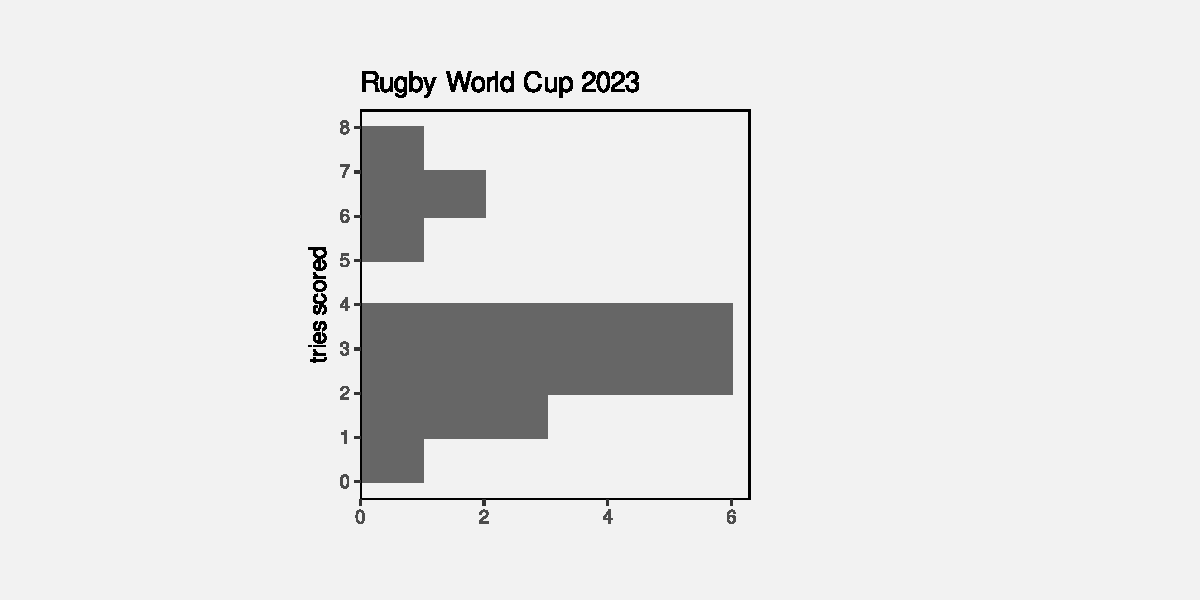
\includegraphics[width=1\linewidth,height=\textheight,keepaspectratio]{index_files/mediabag/text_files/figure-pdf/fig-tries-hist-1.pdf}

}

\caption{\label{fig-tries-hist}A histogram of the number of tries
scored. The bars are horizontal for easy comparison with the
stem-and-leaf plot.}

\end{figure}%

Figure Figure~\ref{fig-tries-stem} shows a stem-and-leaf diagram of the
same data (with tries scored rounded to one decimal place). The data
symbol in this case is a text digit. Every team is encoded as a digit
from 0 to 9, which represents the first decimal place for the average
number of tries scored by each team. For example, New Zealand scored 7.0
tries per game on average and that is encoded as a \texttt{0} beside the
\texttt{7} on the y-axis. The number of tries is also encoded as a
combination of vertical position (the whole number of tries) and
horizontal position (teams with the same whole number of tries are
stacked horizontally, but also ordered by the first decimal place
value).

The number of teams within each range (0 to 1, 1 to 2, etc) is encoded
by the number of digits. Another way to look at it is that the data
symbol is a piece of text consisting of several digits and the number of
teams is encoded as the \textbf{length} of the piece of text.

As with the histogram in Figure~\ref{fig-tries-hist}, there are emergent
shapes with two distinct humps visible, one taller than the other.
However, in Figure~\ref{fig-tries-stem} we are able to decode the raw
data values as well. Furthermore, because the data symbols are text
digits, we are able to decode individual data values very accurately.

In summary, Figure~\ref{fig-tries-stem} combines standard decodings
(\textbf{length}) with \textbf{learned decodings} (text shape) to
provide access to both high-level features of data summaries \emph{and}
raw data values.

\begin{figure}

\centering{

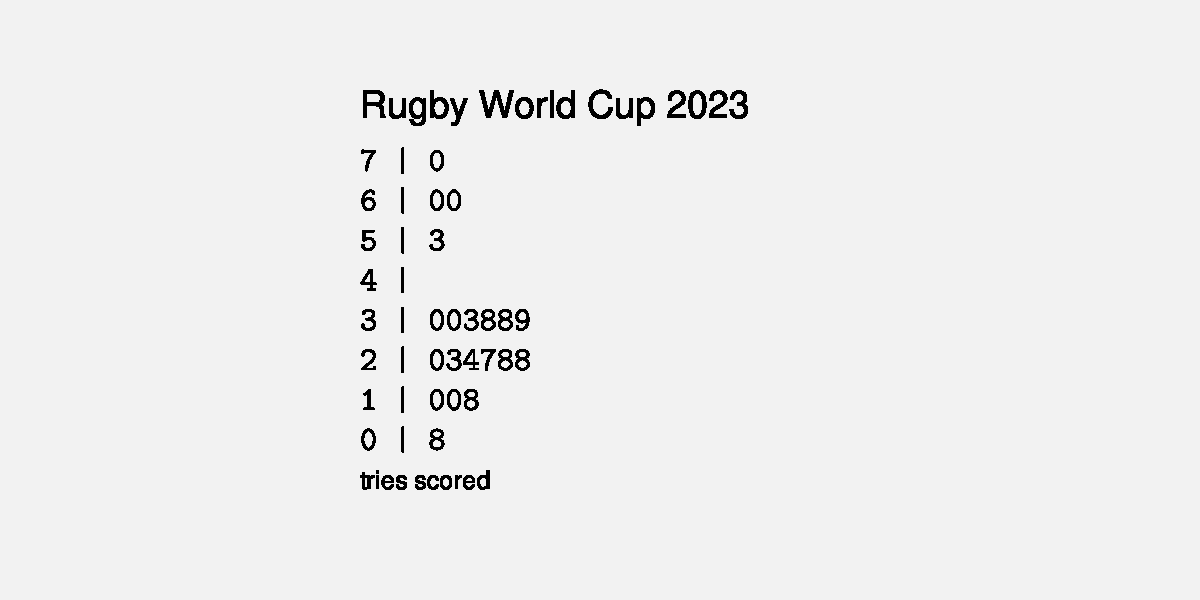
\includegraphics[width=1\linewidth,height=\textheight,keepaspectratio]{index_files/mediabag/text_files/figure-pdf/fig-tries-stem-1.pdf}

}

\caption{\label{fig-tries-stem}A stem-and-leaf plot of the number of
tries scored.}

\end{figure}%

Figure~\ref{fig-tries-stem-colour} shows a variation on
Figure~\ref{fig-tries-stem} with the hemisphere encoded as the colours
of the digits. This provides another demonstration that we can use
simple visual features like colour to encode data values with text data
symbols.

\begin{figure}

\centering{

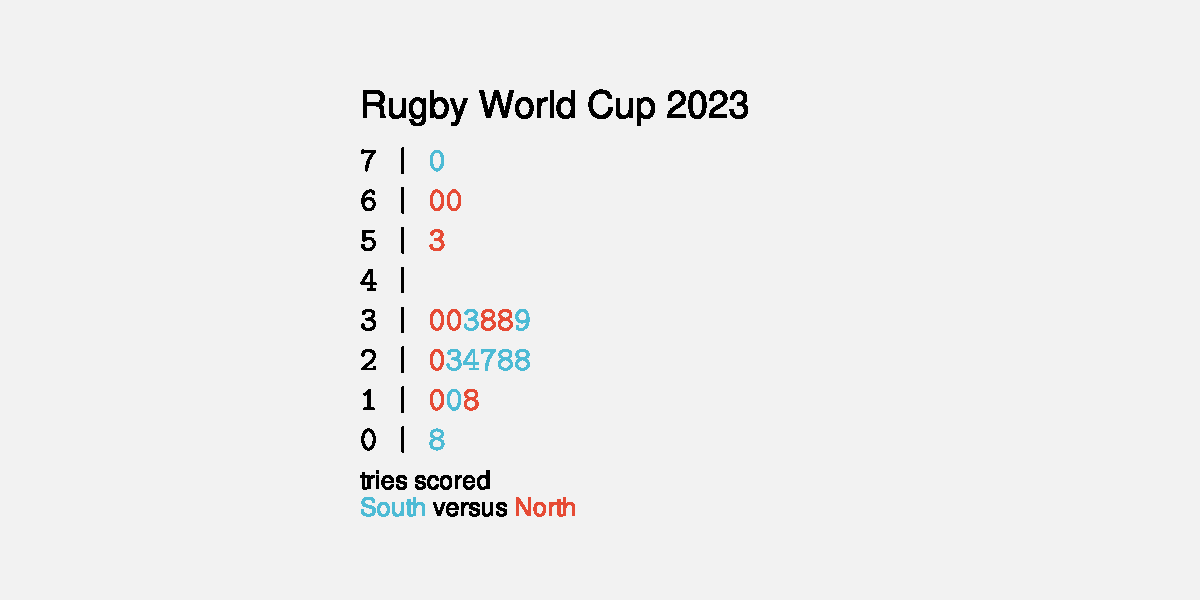
\includegraphics[width=1\linewidth,height=\textheight,keepaspectratio]{index_files/mediabag/text_files/figure-pdf/fig-tries-stem-colour-1.pdf}

}

\caption{\label{fig-tries-stem-colour}A stem-and-leaf plot of the number
of tries scored with hemisphere encoded as colour.}

\end{figure}%

Figure~\ref{fig-tries-stem-weight} shows another variation on
Figure~\ref{fig-tries-stem}, this time with the hemisphere encoded as
the \textbf{weight} of the digits. This demonstrates the idea that there
are text-specific visual features that can be used to encode data
values. Other examples are font family (e.g., Arial versus Roman) and
font slant (italic versus upright).\footnote{(Brath and Banissi 2014) at
  least}

\begin{figure}

\centering{

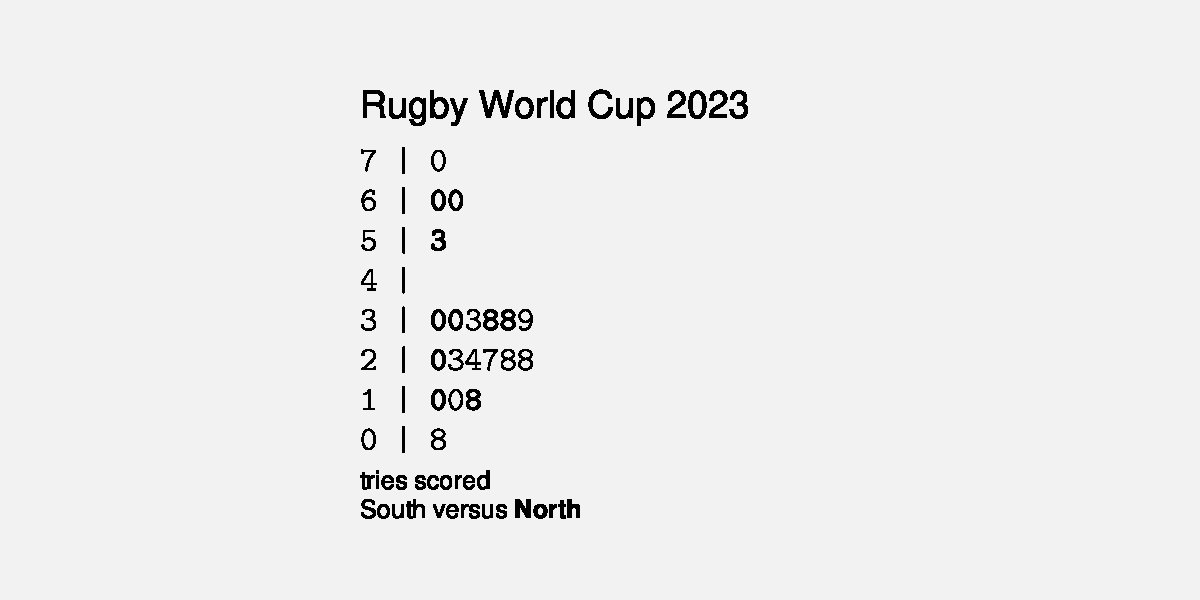
\includegraphics[width=1\linewidth,height=\textheight,keepaspectratio]{index_files/mediabag/text_files/figure-pdf/fig-tries-stem-weight-1.pdf}

}

\caption{\label{fig-tries-stem-weight}A stem-and-leaf plot of the number
of tries scored with hemisphere encoded as font weight.}

\end{figure}%

Stem-and-leaf plots might be seen as an archaic form of data
visualisation, but we can see that they are effective in many
ways.\footnote{Quote from John Tukey about stem-and-leaf plots:

  If we are going to make a mark, it may as well be a meaningful one.
  The simplest - and most useful - meaningful mark is a digit.

  Attributed to ``Some Graphic and Semigraphic Displays'' in T. A.
  Bancroft, ed.~Statistical Papers in Honor of George W. Snedecor (Ames,
  Iowa, 1972), p.~296.}

Unfortunately, despite all of their advantages, stem-and-leaf plots have
a limited usefulness because they can only accommodate very small data
sets. There is a similarity between a stem-and-leaf plot and the stacked
icon plot in Figure~\ref{fig-pic-icon-1}. However, whereas an icon can
easily be used to represent some multiple of objects, that option is not
available for text digits.

\section{Dangers of text}\label{dangers-of-text}

Figure~\ref{fig-text-danger} shows a data visualisation of the number of
gun deaths in Florida between 1990 and 2012, covering the enactment of
Florida's ``stand your ground'' law that loosened the constrainst on an
individual's rights to use deadly force.\footnote{Based on a
  \href{https://www.businessinsider.com/gun-deaths-in-florida-increased-with-stand-your-ground-2014-2}{Business
  Insider} data visualisation; data from
  \href{https://usafacts.org/data/topics/security-safety/crime-and-justice/firearms/firearm-deaths/}{USA
  Facts}.} The title of the plot points out that gun deaths
\emph{decreased} after the law was enacted, which is perhaps surprising
given that use of deadly force was less constrained after the
introduction of the law.

\begin{figure}

\centering{

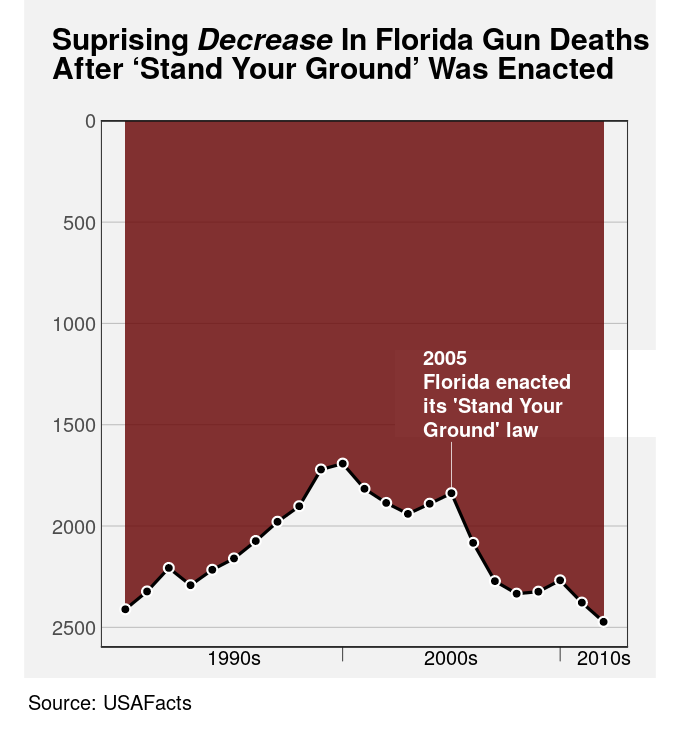
\includegraphics[width=0.5\linewidth,height=\textheight,keepaspectratio]{Images/deaths-florida-contra.png}

}

\caption{\label{fig-text-danger}The title influences our perception; the
message from the data symbols is actually quite different.}

\end{figure}%

However, if we look closely at the plot itself, we can see that the
y-axis scale is inverted. A downward trend is actually an
\emph{increase} in gun deaths, so the data shows that gun deaths
actually increased after the law was enacted.

This example demonstrates that the text within a data visualisation is
not only given a lot of attention, but it can have a dominant effect on
the message that the viewer takes away.\footnote{``Trust and Recall of
  Information across Varying Degrees of Title-Visualization
  Misalignment'' Kong et al (2019) Greater impact that can even override
  message in data. ``Towards Understanding How Readers Integrate Charts
  and Captions: A Case Study with Line Charts'' Kim et al (2021) Studied
  what happens when caption and text are incoherent; viewer goes with
  the prominent visual feature. Main message is to make the text and
  chart coherent.}

Figure~\ref{fig-text-danger} is an example of a deliberately misleading
data visualisation, which we obviously want to avoid. However, the
broader point is that we need to be at least as careful with our choice
of text content as we are with our selection of mappings from data
values to visual features and we have a responsibility to work hard to
make sure that the message from data symbols and from text labels is
completely consistent.

\section{Alt text}\label{alt-text}

Is a data visualisation effective if we cannot see it? We saw in
Section~\ref{sec-CVD} that a data visualisation may not be effective if
a colour encoding does not take into account red-green colour blindness.
But what about a low-vision or blind audience?

Although data visualisation is based on the visual system, it is still
possible to make a data visualisation effective for a low-vision or
blind audience by providing a text description of the data
visualisation. Alt text is a text description of a data visualisation
that will be recognised and read out by a screen reader.

The alt text for a data visualisation will ideally describe what
variables are being displayed and how they are encoded (what sort of
plot is it), data summaries like trends, clusters, outliers, and
correlations, and include the main message of the visualisation,
including causal explanations and wider implications.\footnote{``Accessible
  Visualization via Natural Language Descriptions: A Four-Level Model of
  Semantic Content'' Lundgard and Satyanarayan (2022)}

Another option sometimes employed is to provide tables of data in
addition to the data visualisation, though this will not always be
possible or practical.

All of the images in this document have alt text (or at least they
should!).

\section{Summary}\label{summary-12}

Data values can be encoded as the visual features of text, such as
position and colour, just like for other data symbols.

The shape of text---the characters used in text---is particularly
important because we have a learned decoding of text. We can read data
values from text.

We can use text to encode any type of data, we can represent a very
large number of different categories, and we can decode individual data
values from text extremely accurately.

On the other hand, decoding a large number of data values from text is
very slow and we cannot generate visual summaries from text.

Guides are really just collections of data symbols, with specific data
values encoded as the visual features to demonstrate how data values
have been encoded.

The text elements within guides are essential because they provide the
only precise decoding of exact data values. This is what allows the
decoding of the main data symbols within a data visualisation.

Overall, text is very valuable in a data visualisation for accurately
encoding a small number of data values, or to express complex
information. But text is not appropriate for representing a large number
of raw data values.\footnote{Acknowledge Ware 4th Ed: G8.18 (p327)
  ``When a large number of data points must be represented in a
  visualization, use sybmols instead of words or pictorial icons.''
  G8.19 (p327) ``Use words directly on the chart where the number of
  symbolic objects in each category is relatively few and where space is
  available.''}

\begin{center}\rule{0.5\linewidth}{0.5pt}\end{center}

\theendnotes

\bookmarksetup{startatroot}

\chapter{Mapping Structure}\label{mapping-structure}

Figure~\ref{fig-yji} shows a line plot of the rate of youth crime in New
Zealand for different ethnic groups and a pie chart showing the
proportions of different types of crime.\footnote{Based on figures from
  the Youth Justice Indicators Report from 2021
  \href{https://www.justice.govt.nz/justice-sector-policy/research-data/justice-statistics/youth-justice-indicators/}{}.}
There is a problem with this figure because the line plot and the pie
chart share the same colour palette even though they are visualising
different variables (ethnicity and crime type). For example, the ethnic
group \texttt{European/Other} is encoded as the orange colour of a line
\emph{and} the crime type \texttt{Theft} is also encoded as an orange
colour, in this case of a wedge.

\begin{figure}

\centering{

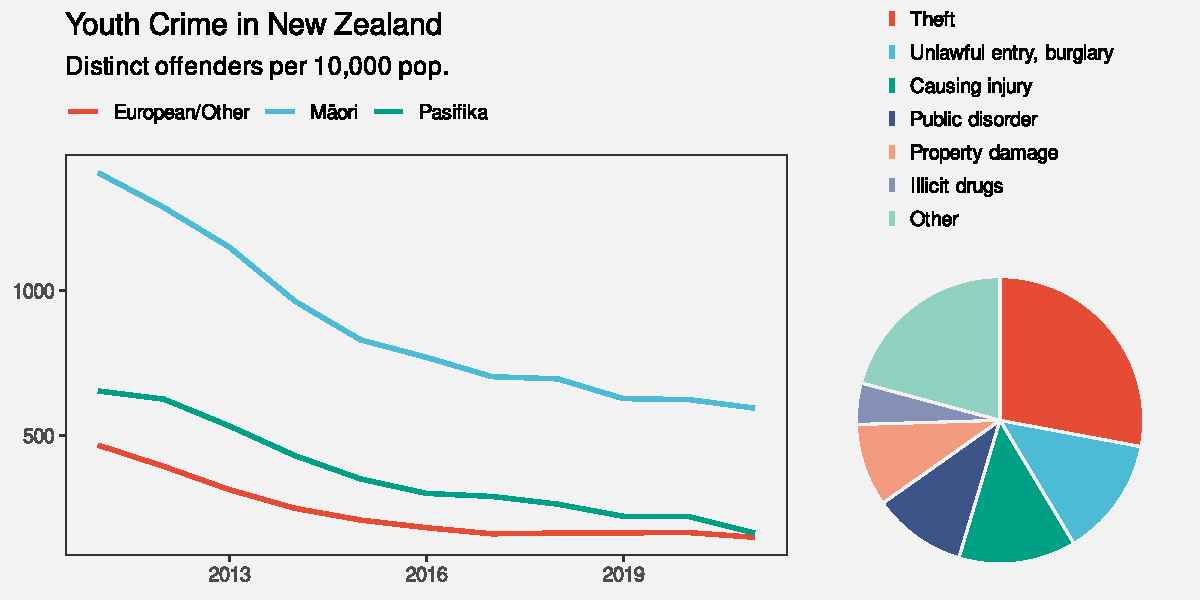
\includegraphics[width=1\linewidth,height=\textheight,keepaspectratio]{index_files/mediabag/design_files/figure-pdf/fig-yji-1.pdf}

}

\caption{\label{fig-yji}}

\end{figure}%

This creates a confusing data visualisation because the same visual
feature possesses multiple conflicting decodings
(Figure~\ref{fig-conflict-decode}). There is nothing wrong with the
encodings in the line plot by itself or with the encodings in the pie
chart by itself, but the overall combination of elements within
Figure~\ref{fig-yji} is ineffective.

\begin{figure}

\centering{

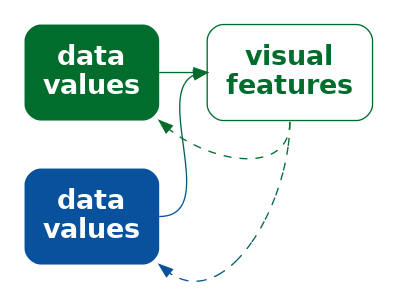
\includegraphics[scale=0.5]{Diagrams/conflict-decode.png}

}

\caption{\label{fig-conflict-decode}If we encode more than one data
value to the same visual feature, it is unclear which is the correct
decoding.}

\end{figure}%

In this section we look at the overall arrangement and coordination of
the elements of a data visualisation.\footnote{Acknowledge that many of
  these ideas align with the ideas of contrast, repetition, alignment,
  and proximity that are espoused in Naomi Robbins book.}

\section{Mapping organisation}\label{sec-map-org}

Figure~\ref{fig-rep-guide} shows a scatter plot of the number of clean
breaks and the number of tries for countries at the 2023 Rugby World Cup
(Table~\ref{tbl-rwc-2023}). This data visualisation is similar to
Figure~\ref{fig-scatter}, but with an additional encoding of the
hemisphere for each country as the colour of the data points.

The legend (guide) in Figure~\ref{fig-rep-guide} demonstrates the scale
for the colour encoding: which colour is used to encode each hemisphere.
In Section~\ref{sec-guides}, we described how the proximity of the
labels ``South'' and ``North'' to the coloured points in the legend
allow us to associate the colours with the different hemispheres. The
different values of hemisphere are encoded as the vertical positions of
the points and the text labels; both the orange point and the label
``South'' have the same vertical position.

\begin{figure}

\centering{

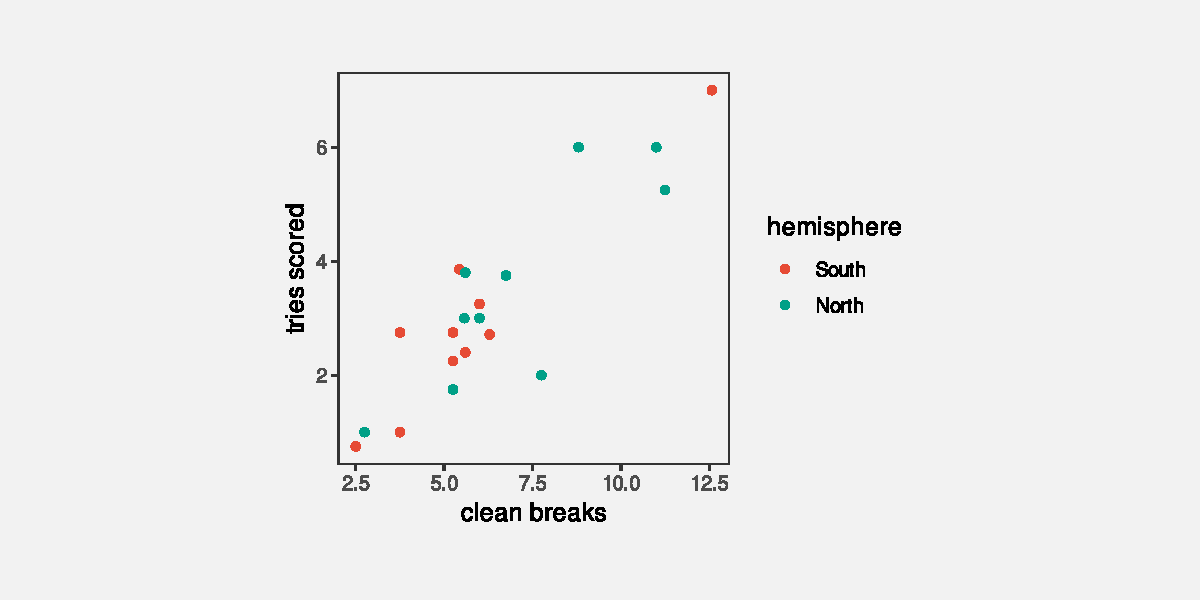
\includegraphics[width=1\linewidth,height=\textheight,keepaspectratio]{index_files/mediabag/design_files/figure-pdf/fig-rep-guide-1.pdf}

}

\caption{\label{fig-rep-guide}A scatter plot of the number of times a
team breaks through the opposition defence and the number of tries that
a team scores (both are per-game averages) for teams at the 2023 Rugby
World Cup.}

\end{figure}%

What about the horizontal position of the points and the text in the
legend? These do not encode hemisphere values because they are the same
for both North and South. What about the position of the legend title,
``hemisphere''?

All of the elements of the legend are positioned together and to the
right of the main plot. Their proximity to each other (and separation
from the main plot) mean that we see the legend as a separate group
(Section~\ref{sec-visual-model-groups}). This creates a visual
organisation for the plot, which helps the viewer to navigate and
comprehend the different elements of the plot (could do with a CITE
here). This is analogous to reading a body of text, which is split into
paragraphs and sections with headings to help the reader navigate the
text.

One way to express this is that the \textbf{position} of the elements of
the legend \textbf{encode} the \textbf{organisation} of the overall data
visualisation. Our visual system \textbf{decodes} the legend as a
separate element based on the proximity of the text and points in the
legend.

Another way to say it is that each element of the data visualisation in
Figure~\ref{fig-rep-guide} belongs to one of two groups: the main plot
or the legend. There is a \textbf{qualitative} value, \texttt{plot} or
\texttt{legend}, associated with each element of the data visualisation.
These qualitative values are encoded as the \textbf{position} of the
elements within the data visualisation: on the left or on the right.

\begin{figure}

\centering{

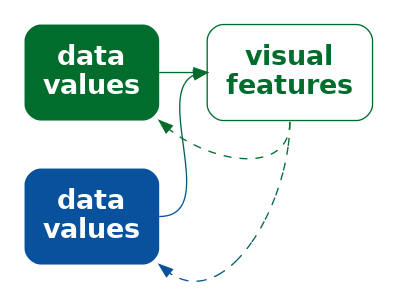
\includegraphics[scale=0.5]{Diagrams/conflict-decode.png}

}

\caption{\label{fig-org-vis-decode}We can encode the structure of a data
visualisation as position so that elements that are part of the same
structure are close to each other.}

\end{figure}%

\begin{quote}
An effective data visualisation has to convey information about how to
read the plot as well as information about the data itself.
\end{quote}

\begin{quote}
The structure or organisation of a data visualisation is a qualitative
value that can be effectively encoded as the position of different
elements.
\end{quote}

Figure~\ref{fig-align} shows a variation of Figure~\ref{fig-rep-guide},
with exactly the same plot elements, but in a different arrangement.
There is greater separation of the legend from the main plot. The legend
has also been moved so that its top is aligned with the top of the main
plot. Similarly, the axis titles have been moved so that they align with
the top and right sides of the plot, and the y-axis label has been
rotated to horizontal. More subtly, the right edge of the y-axis label
is aligned with the right edge of the y-axis tick labels and the points
in the legend are aligned with the left edge of the legend title.

\begin{figure}

\centering{

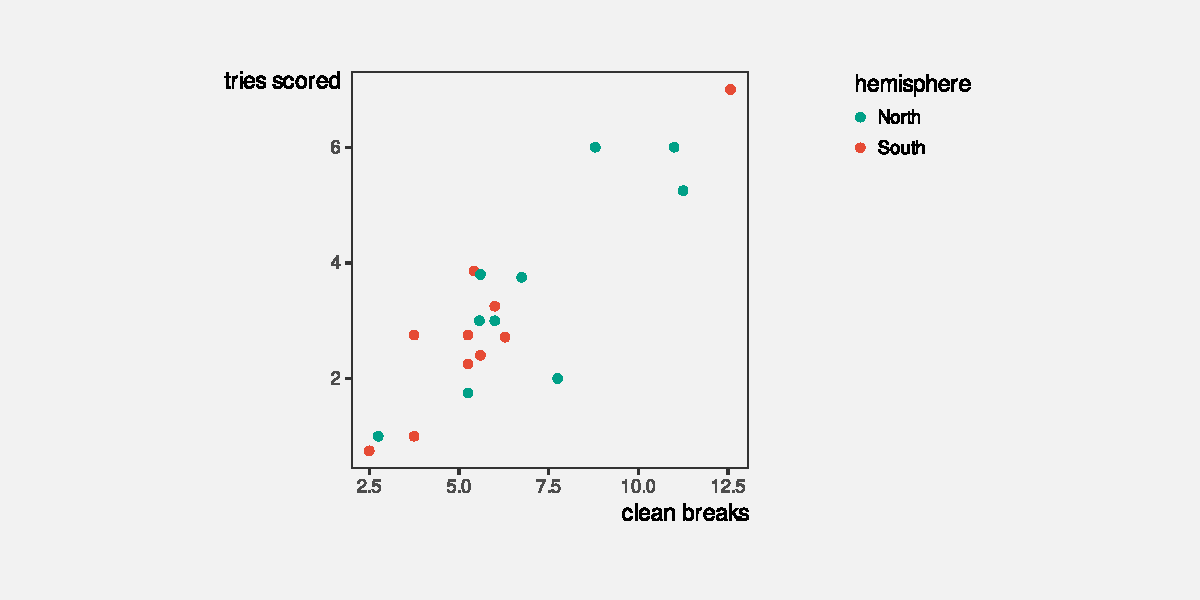
\includegraphics[width=1\linewidth,height=\textheight,keepaspectratio]{index_files/mediabag/design_files/figure-pdf/fig-align-1.pdf}

}

\caption{\label{fig-align}A scatter plot of the number of times a team
breaks through the opposition defence and the number of tries that a
team scores (both are per-game averages) for teams at the 2023 Rugby
World Cup.}

\end{figure}%

All of these changes are aimed at making the data visualisation more
orderly (Section~\ref{sec-simplicity}). The legend is more obviously a
separate element from the main plot and the axis titles more obviously
connect to the main plot. A more orderly arrangement of the visual
elements will provide fewer distractions and lead to a more effective
data visualisation because the important differences in the data will be
more readily perceived (Section~\ref{sec-differences}).

The strong alignment and regular patterns within facetted plots like
Figure~\ref{fig-facet-after} are another effective example of keeping
everything else the same in order to champion the changes in the data.
Conversely, another weakness of placing data symbols on maps, like in
Figure~\ref{fig-map-alt-2}, is the distracting complexity that results.

\section{Consistent mappings}\label{consistent-mappings}

Figure~\ref{fig-rep-none} shows a variation on
Figure~\ref{fig-rep-guide} with a modified legend. In this plot, the
hemisphere of a country is encoded using orange and green within the
main plot, but then hemisphere is encoded using light blue and brown in
the legend. This is clearly an ineffective data visualisation, but it
highlights the importance of maintaining consistent mappings between
different elements of a plot.\footnote{This particularly echoes the
  repetition part of CRAP design.}

\begin{figure}

\centering{

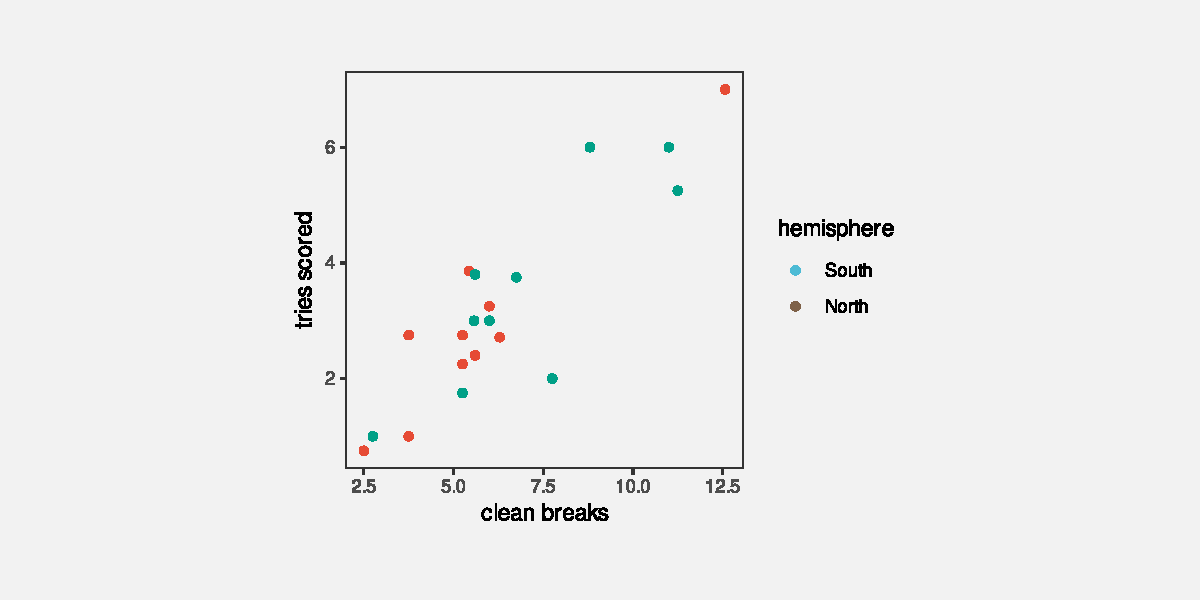
\includegraphics[width=1\linewidth,height=\textheight,keepaspectratio]{index_files/mediabag/design_files/figure-pdf/fig-rep-none-1.pdf}

}

\caption{\label{fig-rep-none}A scatter plot of the number of times a
team breaks through the opposition defence and the number of tries that
a team scores (both are per-game averages) for teams at the 2023 Rugby
World Cup.}

\end{figure}%

Figure~\ref{fig-rep-double} demonstrates that we can harness consistent
mappings to improve upon the original Figure~\ref{fig-rep-guide}. In
this plot, the encoding of hemisphere as the colour of points is not
only consistent between the main plot and the legend, but it has been
extended to the colour of legend text. The visual grouping of elements
that relate to the same hemisphere is now stronger within the legend and
across the entire data visualisation
(Section~\ref{sec-visual-model-groups}).

\begin{figure}

\centering{

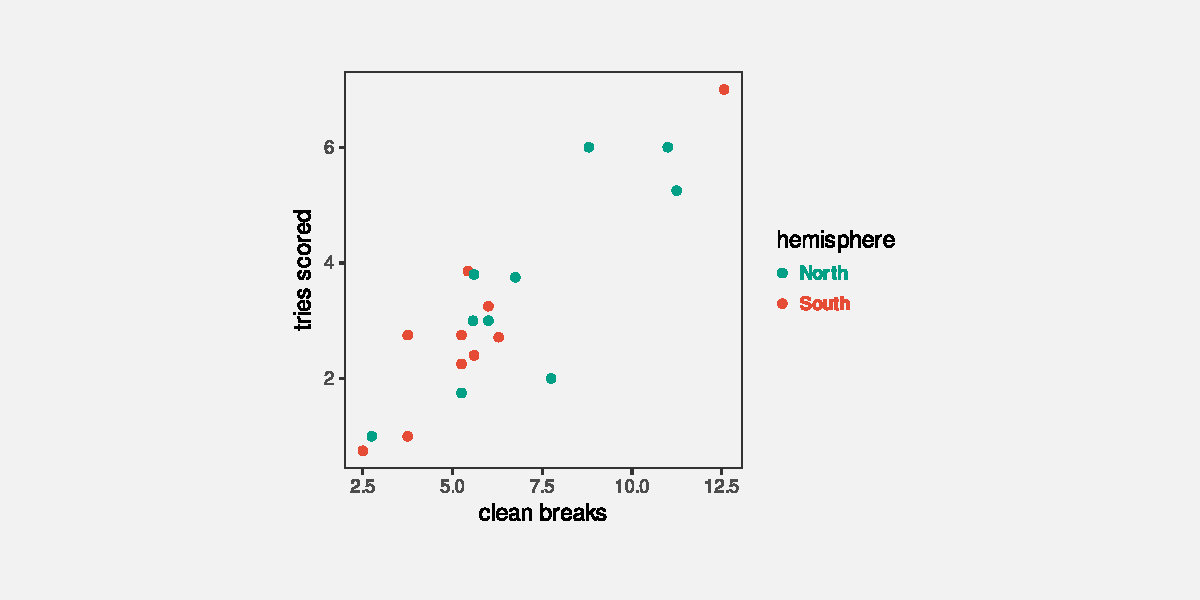
\includegraphics[width=1\linewidth,height=\textheight,keepaspectratio]{index_files/mediabag/design_files/figure-pdf/fig-rep-double-1.pdf}

}

\caption{\label{fig-rep-double}A scatter plot of the number of times a
team breaks through the opposition defence and the number of tries that
a team scores (both are per-game averages) for teams at the 2023 Rugby
World Cup.}

\end{figure}%

\section{The dangers of inconsistent
mappings}\label{the-dangers-of-inconsistent-mappings}

Figure~\ref{fig-trump-bill} shows a bar plot of the impact of a proposed
tax bill during the second Trump administration.\footnote{Based on plot
  from ``Popular Information'' web site (Judd Legum)
  https://popular.info/p/the-ugly-truth-about-trumps-big-beautiful Data
  source: Penn Wharton Budget Model
  https://budgetmodel.wharton.upenn.edu/estimates/2025/5/16/distributional-effects-of-house-budget-reconciliation-as-of-thursday-may-15}
Each bar represents a change in income for a particular income bracket.
Lower incomes are to the left and higher incomes are to the right. There
are labels to describe each income bracket and there are labels that
describe each change in income. Where the change in income is large, the
label for change in income is written within the bar (at the top of the
bar), but for smaller changes in income, the bar is too small to fit the
label, so the label is placed just above the bar. For the two leftmost
bars, the change in income is actually negative and the change in income
label is placed \emph{below} the bar. The labels that describe the
income brackets are mostly below the bars, but for the two leftmost bars
the labels for the income brackets are placed above the bars.

In summary, there are two labels for each bar, one below the bar and one
above (or at the top of) the bar. This consistent positioning of the
labels encourages the viewer to decode two groups of labels: one group
above the bars and one group below the bars. This can mislead us into
comparing, for example, ``-1K'' for the leftmost bar with ``4.3M'' for
the rightmost bar, when the correct comparison is between ``-1K'' (for
the lowest income bracket) and ``389.3K'' (for the highest income
bracket).\footnote{This is precisely the mistake that was made when this
  data visualisation was discussed on
  \href{https://www.youtube.com/watch?v=AQiukyzB6x0}{The Majority Report
  (\textasciitilde6:00)}.}

Just as it makes no sense to change the encoding of data values within a
data visualisation (Figure~\ref{fig-rep-none}) or across multiple data
visualisations within the same document (Figure~\ref{fig-yji}), it makes
no sense to change the encoding of structure within a data
visualisation.

\begin{figure}

\centering{

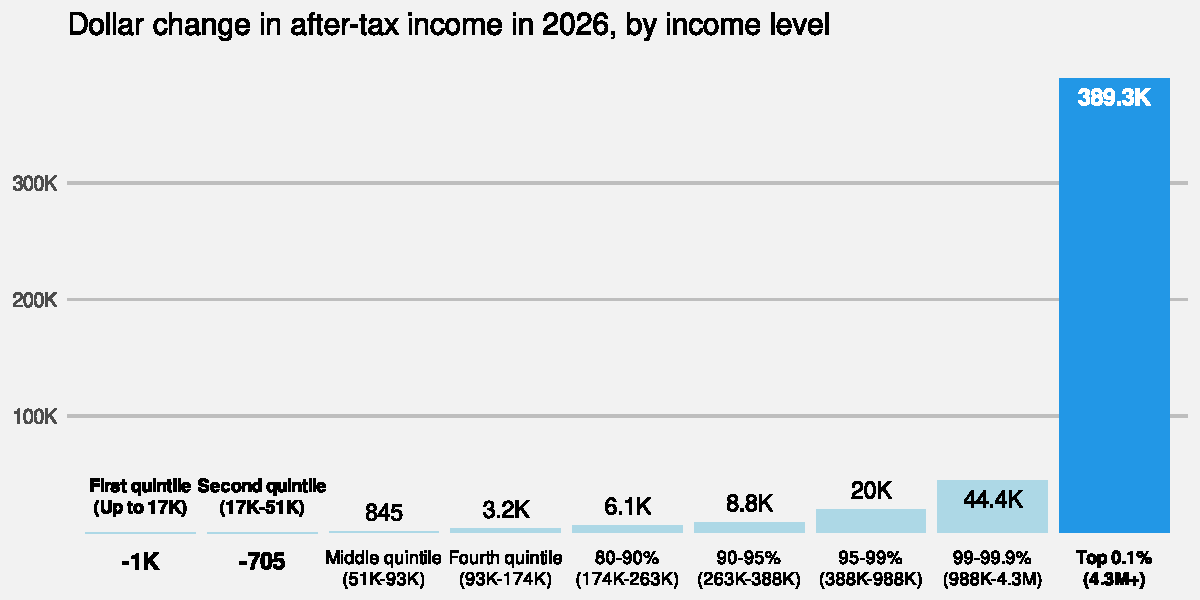
\includegraphics[width=1\linewidth,height=\textheight,keepaspectratio]{index_files/mediabag/design_files/figure-pdf/fig-trump-bill-1.pdf}

}

\caption[\label{fig-trump-bill}A bar plot of the distributional effects
of Trump's ``Big, Beautiful Bill''.]{\label{fig-trump-bill}A bar plot of the distributional effects
of Trump's ``Big, Beautiful Bill''.\footnotemark{}}

\end{figure}%
\footnotetext{Based on plot from
  ``Popular Information'' web site (Judd Legum)
  https://popular.info/p/the-ugly-truth-about-trumps-big-beautiful Data
  source: Penn Wharton Budget Model
  https://budgetmodel.wharton.upenn.edu/estimates/2025/5/16/distributional-effects-of-house-budget-reconciliation-as-of-thursday-may-15}

\section{Mapping importance}\label{mapping-importance}

Figure~\ref{fig-contrast} shows a variation on
Figure~\ref{fig-rep-double} with many elements of the plot drawn in
light grey. The effect of this change is to create two visual groups,
one lighter and less saturated than the other. This emphasises the main
data symbols in the main plot and in the legend, and de-emphasises the
axes and labels. Our attention is drawn to the darker and more saturated
elements first (Section~\ref{sec-attention}), with the other elements in
the background, which we can focus on if we need the additional
information.\footnote{CRAP contrast}

By comparison, in Figure~\ref{fig-rep-double} there is a similar visual
impact from all elements of the plot, so it is less clear where to look
first. All of the elements of the data visualisation compete for our
attention.

This is another example of encoding (qualitative) non-data values as
visual features (see Section~\ref{sec-map-org}). In this case, we are
encoding the \textbf{importance} of different visual elements as visual
features, in this case colour. We decode the differences in colour to a
more important group of elements and a less important group of elements.

\begin{figure}

\centering{

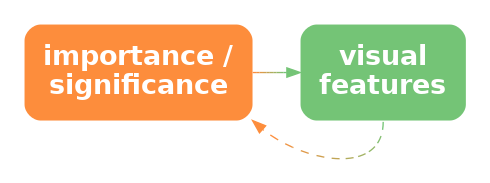
\includegraphics[scale=0.5]{Diagrams/imp-vis-decode.png}

}

\caption{\label{fig-imp-vis-decode}We can encode the importance of
elements within a data visualisation as visual features so that elements
that are more important are more visible.}

\end{figure}%

\begin{figure}

\centering{

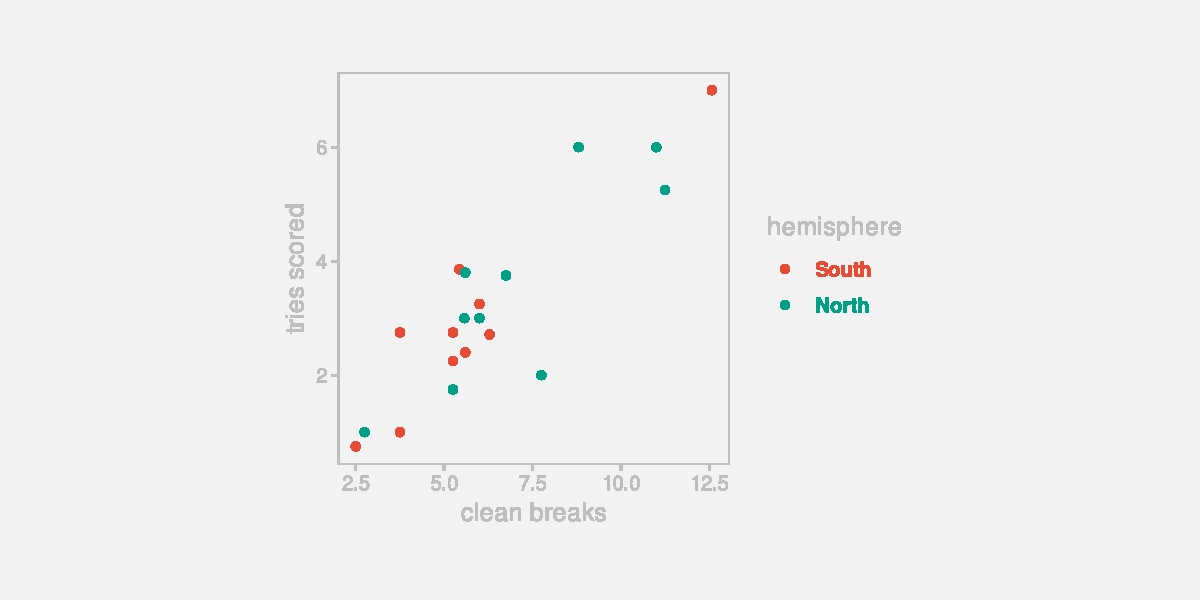
\includegraphics[width=1\linewidth,height=\textheight,keepaspectratio]{index_files/mediabag/design_files/figure-pdf/fig-contrast-1.pdf}

}

\caption{\label{fig-contrast}A scatter plot of the number of times a
team breaks through the opposition defence and the number of tries that
a team scores (both are per-game averages) for teams at the 2023 Rugby
World Cup.}

\end{figure}%

Figure~\ref{fig-highlight} shows a similar application of importance. In
this case, we are highlighting two data points (New Zealand and South
Africa). The distinct colour and larger size of the two points encodes
the importance of those points and draws attention to those points, with
everything else as background context.

\begin{figure}

\centering{

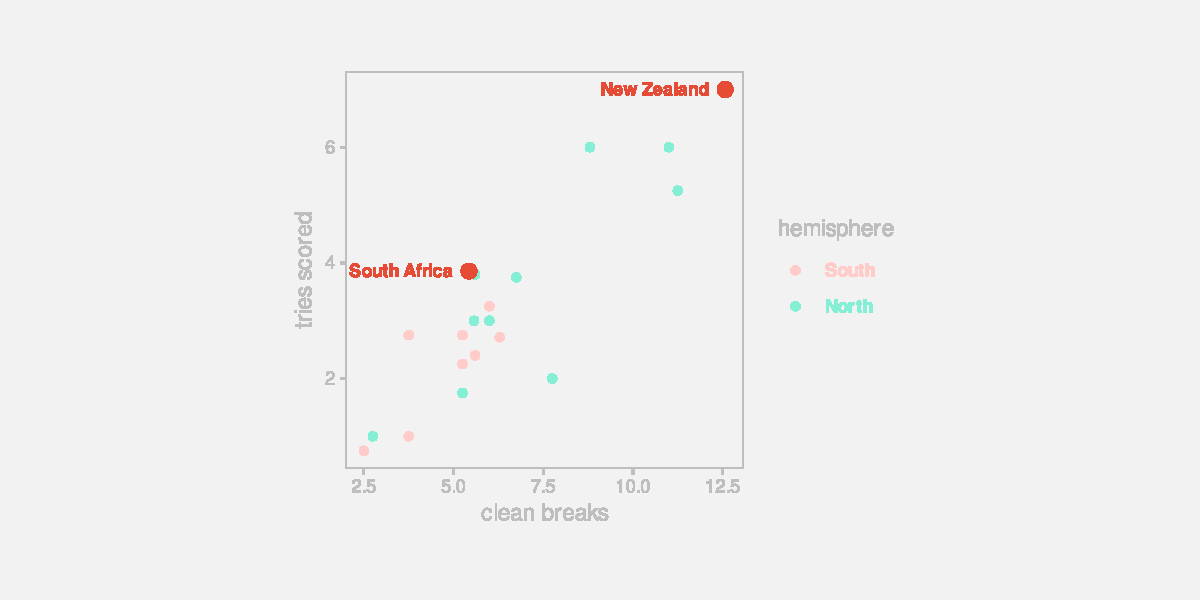
\includegraphics[width=1\linewidth,height=\textheight,keepaspectratio]{index_files/mediabag/design_files/figure-pdf/fig-highlight-1.pdf}

}

\caption{\label{fig-highlight}A scatter plot of the number of times a
team breaks through the opposition defence and the number of tries that
a team scores (both are per-game averages) for teams at the 2023 Rugby
World Cup.}

\end{figure}%

Section~\ref{sec-differences}

\section{Distractions}\label{distractions}

Add examples of making the WRONG thing important (e.g., use thick lines
on bar borders or bright colours on unimportant elements) ?

Refer back to chart junk and clutter (Section~\ref{sec-junk}).

\section{Summary}\label{summary-13}

Just as we can map data values to visual features, to communicate
information about the data, we can map non-data information to visual
features, to communicate important aspects of the structure of a data
visualisation.

Communicating structure helps the viewer to navigate within a data
visualisation.

Position is especially important

\begin{center}\rule{0.5\linewidth}{0.5pt}\end{center}

\theendnotes

\bookmarksetup{startatroot}

\chapter*{Review}\label{sec-review}
\addcontentsline{toc}{chapter}{Review}

\markboth{Review}{Review}

Add review at the end that reinforces the threads like visual feature,
visual shape, visual object and mappings

Present process by which a data vis can be broken down. What data
symbols are being used? (simple or complex) What mappings are being
used? What do we want to decode? (data or summaries) If mapping back to
raw data, are the mappings accurate? What can be mapped back to? Are
mappings congruent with data? \ldots{}

\begin{itemize}
\item
  Use heatmap as case study?
\item
  do the side-by-side pie chart idea as an example of reasoning your way
  to a new visualisation.
\item
  Move the discussion/revisit of tables from text section to here ?
\item
  Another possible application of data vis knowledge: Analyse one of the
  weird boxplot variations that look a bit like a ziggurat?
\end{itemize}

List of questions to evaluate a data vis (maybe nest these a bit):

\begin{itemize}
\item
  What are the data variables
\item
  What visual features are they mapped to
\item
  What type of data
\item
  Can the visual features represent the data
\item
  Is there the capacity to represent all categories
\item
  How accurate are the decodings
\item
  Is there congruence or dissonance in the mapping
\item
  Mapping data or data summary
\item
  Do visual features interact
\item
  Are there emergent features
\item
  Is the data symbol a visual shape
\item
  Is that appropriate
\item
  A visual object
\item
  Is that appropriate
\item
  Learned mappings somehow (distinct from implicit mappings)
\item
  Do all visual differences correspond to differences in the data?
\item
  Are all differences in the data represented by visual differences?
\item
  Does each data value map to its own data symbol If not, individual
  data values may be difficult to decode
\item
  Do multiple data values map to a single data symbol If not, data
  summaries may be difficult to decode
\end{itemize}

And so on \ldots{}

\phantomsection\label{refs}
\begin{CSLReferences}{1}{0}
\bibitem[\citeproctext]{ref-bertini-how-not-to-lie}
Bertini, Enrico. 2025. {``How NOT to Lie with Charts.''}
\url{https://filwd.substack.com/p/how-not-to-lie-with-charts}.

\bibitem[\citeproctext]{ref-DBLP:journalsux2fcorrux2fabs-2008-11310}
Bertini, Enrico, Michael Correll, and Steven Franconeri. 2020. {``Why
Shouldn't All Charts Be Scatter Plots? Beyond Precision-Driven
Visualizations.''} \emph{CoRR} abs/2008.11310.
\url{https://arxiv.org/abs/2008.11310}.

\bibitem[\citeproctext]{ref-boring1942sensation}
Boring, Edwin G. 1942. \emph{Sensation and Perception in the History of
Experimental Psychology}. Appleton-Century-Crofts.

\bibitem[\citeproctext]{ref-rNOMADS}
Bowman, Daniel C., and Jonathan M. Lees. 2015. {``Near Real Time Weather
and Ocean Model Data Access with {rNOMADS}.''} \emph{Computers \&
Geosciences} 78: 88--95.
\url{https://doi.org/10.1016/j.cageo.2015.02.013}.

\bibitem[\citeproctext]{ref-brath2014design}
Brath, Richard, and Ebad Banissi. 2014. {``The Design Space of
Typeface.''} In \emph{18th International Conference on Information
Visualisation (IV)}, 41--50. Paris, France: IEEE.
\url{https://doi.org/10.1109/IV.2014.17}.

\bibitem[\citeproctext]{ref-cairo2012functional}
Cairo, Alberto. 2012. \emph{The Functional Art: An Introduction to
Information Graphics and Visualization}. New Riders.

\bibitem[\citeproctext]{ref-CairoAlberto2014Eiid}
---------. 2014. {``Ethical Infographics: In Data Visualization,
Journalism Meets Engineering.''} \emph{The IRE Journal} 37 (2): 25.

\bibitem[\citeproctext]{ref-cairo2016truthful}
---------. 2016. \emph{The Truthful Art: Data, Charts, and Maps for
Communication}. 1st ed. San\,Francisco, CA: New Riders.

\bibitem[\citeproctext]{ref-cairo2019howchartslie}
---------. 2019. \emph{How Charts Lie: Getting Smarter about Visual
Information}. First. New York: W.~W. Norton \& Company.

\bibitem[\citeproctext]{ref-chernoff1973faces}
Chernoff, Herman. 1973. {``The Use of Faces to Represent Points in
k-Dimensional Space Graphically.''} \emph{Journal of the American
Statistical Association} 68 (342): 361--68.
\url{https://doi.org/10.1080/01621459.1973.10482434}.

\bibitem[\citeproctext]{ref-cleveland1985graphical}
Cleveland, William S. 1985a. {``Graphical Methods for Data Presentation:
Full Scale Breaks, Dot Charts, and Multibased Logging.''} \emph{The
American Statistician} 39 (4): 270--80.

\bibitem[\citeproctext]{ref-cleveland1985elements}
Cleveland, William S. 1985b. \emph{The Elements of Graphing Data}.
Monterey, CA: Wadsworth Advanced Books; Software.

\bibitem[\citeproctext]{ref-cleveland1993visualizing}
---------. 1993. \emph{Visualizing Data}. Summit, NJ: Hobart Press.

\bibitem[\citeproctext]{ref-cleveland1984graphical}
Cleveland, William S, and Robert McGill. 1984. {``Graphical Perception:
Theory, Experimentation, and Application to the Development of Graphical
Methods.''} \emph{Journal of the American Statistical Association} 79
(387): 531--54.

\bibitem[\citeproctext]{ref-wikipedia-visual-system}
contributors, Wikipedia. 2025. {``Visual System.''} In \emph{Wikipedia}.
\url{https://en.wikipedia.org/wiki/Visual_system}.

\bibitem[\citeproctext]{ref-cookSwayne2007}
Cook, Dianne, and Deborah F. Swayne. 2007. \emph{Interactive and Dynamic
Graphics for Data Analysis: With r and GGobi}. 1st ed. Use r! Springer
New York. \url{https://doi.org/10.1007/978-0-387-71762-3}.

\bibitem[\citeproctext]{ref-78044e4a-01f4-3942-91fb-a9f8dacb4e28}
Eells, Walter Crosby. 1926. {``The Relative Merits of Circles and Bars
for Representing Component Parts.''} \emph{Journal of the American
Statistical Association} 21 (154): 119--32.
\url{http://www.jstor.org/stable/2277140}.

\bibitem[\citeproctext]{ref-data_by_design_emory2021}
Emory Digital Humanities Lab. 2021. {``Data\,by\,Design: An Interactive
History of Data Visualization.''} \url{https://dev.dataxdesign.io/}.

\bibitem[\citeproctext]{ref-franconeri2021}
Franconeri, Steven L., Lace M. Padilla, Priti Shah, Jeffrey M. Zacks,
and Jessica Hullman. 2021. {``The Science of Visual Data Communication:
What Works.''} \emph{Psychological Science in the Public Interest} 22
(3): 110--61. \url{https://doi.org/10.1177/15291006211051956}.

\bibitem[\citeproctext]{ref-healy2018data}
Healy, Kieran. 2018. \emph{Data Visualization: A Practical
Introduction}. Princeton, NJ: Princeton University Press.

\bibitem[\citeproctext]{ref-heer2010crowdsourcing}
Heer, Jeffrey, and Michael Bostock. 2010. {``Crowdsourcing Graphical
Perception: Using Mechanical Turk to Assess Visualization Design.''} In
\emph{Proceedings of the SIGCHI Conference on Human Factors in Computing
Systems}, 203--12. ACM.

\bibitem[\citeproctext]{ref-nz-doctor}
Huskinson, Peter. 2024. {``Follow the Money to See What Budget 2024
Spends on Health.''} \emph{New Zealand Doctor Rata Aotearoa}.
\url{https://www.nzdoctor.co.nz/article/opinion/follow-money-see-what-budget-2024-spends-health}.

\bibitem[\citeproctext]{ref-karstenChartsAndGraphs}
Karsten, Karl G. 1925. \emph{Charts and Graphs}. Prentice-Hall.

\bibitem[\citeproctext]{ref-kosslyn1989understanding}
Kosslyn, Stephen M. 1989. {``Understanding Charts and Graphs.''}
\emph{Applied Cognitive Psychology} 3 (3): 185--225.

\bibitem[\citeproctext]{ref-mackinlay1986automatic}
Mackinlay, Jock. 1986. {``Automatic Design of Graphical Presentations of
Relational Information.''} \emph{ACM Transactions on Graphics (TOG)} 5
(2): 110--41.

\bibitem[\citeproctext]{ref-MCKEE198425}
Mckee, Suzanne P., and Ken Nakayama. 1984. {``The Detection of Motion in
the Peripheral Visual Field.''} \emph{Vision Research} 24 (1): 25--32.
https://doi.org/\url{https://doi.org/10.1016/0042-6989(84)90140-8}.

\bibitem[\citeproctext]{ref-munzner2014visualization}
Munzner, Tamara. 2014. \emph{Visualization Analysis and Design}. CRC
Press.

\bibitem[\citeproctext]{ref-pkg-gggrid}
Murrell, Paul. 2022. \emph{Gggrid: Draw with 'Grid' in 'Ggplot2'}.
\url{https://CRAN.R-project.org/package=gggrid}.

\bibitem[\citeproctext]{ref-doi:10.1068ux2fp2985}
Ninio, Jacques, and Kent A Stevens. 2000. {``Variations on the Hermann
Grid: An Extinction Illusion.''} \emph{Perception} 29 (10): 1209--17.
\url{https://doi.org/10.1068/p2985}.

\bibitem[\citeproctext]{ref-owen1999}
Owen, G. Scott, Gitta Domik, Theresa-Marie Rhyne, Ken W. Brodlie, and
Beatriz Sousa Santos. 1999. {``Definitions and Rationale for
Visualization.''}
\url{https://education.siggraph.org/static/HyperVis/visgoals/visgoal2.htm}.

\bibitem[\citeproctext]{ref-pomerantz1994emergent}
Pomerantz, James R., and Anna I. Cragin. 1994. {``Emergent Features and
Feature Combination.''} \emph{Attention, Perception, \& Psychophysics}
55 (1): 48--55.

\bibitem[\citeproctext]{ref-robbins2005creating}
Robbins, Naomi B. 2005. \emph{Creating More Effective Graphs}. Hoboken,
NJ: Wiley-Interscience.

\bibitem[\citeproctext]{ref-annurev:ux2fcontentux2fjournalsux2f10.1146ux2fannurev-vision-082114-035733}
Rosenholtz, Ruth. 2016. {``Capabilities and Limitations of Peripheral
Vision.''} Journal Article. \emph{Annual Review of Vision Science} 2
(Volume 2, 2016): 437--57.
https://doi.org/\url{https://doi.org/10.1146/annurev-vision-082114-035733}.

\bibitem[\citeproctext]{ref-PeripheralVisionACriticalComponentofManyVisualTasks}
---------. 2023. {``Peripheral Vision: A Critical Component of Many
Visual Tasks.''} Oxford University Press.
\url{https://doi.org/10.1093/acrefore/9780190236557.013.878}.

\bibitem[\citeproctext]{ref-schwabish}
Schwabish, Jonathan A. 2020. {``Ten Guidelines for Better Tables.''}
\emph{Journal of Benefit-Cost Analysis} 11 (2): 151--78.

\bibitem[\citeproctext]{ref-Sidiropoulos03072018}
Sidiropoulos, Nikos, Sina Hadi Sohi, Thomas Lin Pedersen, Bo Torben
Porse, Ole Winther, Nicolas Rapin, and Frederik Otzen Bagger and. 2018.
{``SinaPlot: An Enhanced Chart for Simple and Truthful Representation of
Single Observations over Multiple Classes.''} \emph{Journal of
Computational and Graphical Statistics} 27 (3): 673--76.
\url{https://doi.org/10.1080/10618600.2017.1366914}.

\bibitem[\citeproctext]{ref-smil2022how}
Smil, Vaclav. 2022. \emph{How the World Really Works: The Science Behind
How We Got Here and Where We're Going}. New York: Viking.

\bibitem[\citeproctext]{ref-suxf6nning_2022}
Sönning, Lukas. 2022. {``Drawing on Principles of Perception: The Line
Plot.''} PsyArXiv. \url{https://doi.org/10.31234/osf.io/tjfz5}.

\bibitem[\citeproctext]{ref-Suxf6nning2023}
---------. 2023. {``Drawing on Principles of Perception: The Line
Plot.''} In \emph{Data Visualization in Corpus Linguistics: Critical
Reflections and Future Directions}, edited by Lukas Sönning and Ole
Schützler. Studies in Variation, Contacts and Change in English 22.
Helsinki: VARIENG. \url{https://urn.fi/URN:NBN:fi:varieng:series-22-2}.

\bibitem[\citeproctext]{ref-stevens1957psychophysics}
Stevens, Stanley Smith. 1957. {``On the Psychophysical Law.''}
\emph{Psychological Review} 64 (3): 153--81.

\bibitem[\citeproctext]{ref-10.1167ux2fjov.20.12.2}
Stewart, Emma E. M., Matteo Valsecchi, and Alexander C. Schütz. 2020.
{``A Review of Interactions Between Peripheral and Foveal Vision.''}
\emph{Journal of Vision} 20 (12): 2--2.
\url{https://doi.org/10.1167/jov.20.12.2}.

\bibitem[\citeproctext]{ref-talbot2014four}
Talbot, Justin, Heidi Lam, Jock MacKinlay, and Jeffrey Heer. 2014.
{``Four Experiments on the Perception of Bar Charts.''} In \emph{IEEE
Transactions on Visualization and Computer Graphics}, 20:2152--60. 12.
IEEE.

\bibitem[\citeproctext]{ref-theus_urbanek_2008_interactive}
Theus, Martin, and Simon Urbanek. 2008. \emph{Interactive Graphics for
Data Analysis: Principles and Examples}. 1st ed. Boca Raton, FL: Chapman
\& Hall/CRC.

\bibitem[\citeproctext]{ref-tufte1983visual}
Tufte, Edward R. 1983. \emph{The Visual Display of Quantitative
Information}. Cheshire, Connecticut: Graphics Press.

\bibitem[\citeproctext]{ref-tufte1990envisioning}
---------. 1990. \emph{Envisioning Information}. Cheshire, CT: Graphics
Press.

\bibitem[\citeproctext]{ref-tufte1997visual}
---------. 1997. \emph{Visual Explanations: Images and Quantities,
Evidence and Narrative}. Cheshire, CT: Graphics Press.

\bibitem[\citeproctext]{ref-tufte2006beautiful}
---------. 2006. \emph{Beautiful Evidence}. Cheshire, CT: Graphics
Press.

\bibitem[\citeproctext]{ref-TVERSKY2002247}
Tversky, Barbara, Julie Bauer Morrison, and Mireille Betrancourt. 2002.
{``Animation: Can It Facilitate?''} \emph{International Journal of
Human-Computer Studies} 57 (4): 247--62.
https://doi.org/\url{https://doi.org/10.1006/ijhc.2002.1017}.

\bibitem[\citeproctext]{ref-unwinTheusHofmann2006}
Unwin, Antony, Martin Theus, and Heike Hofmann. 2006. \emph{Graphics of
Large Datasets: Visualizing a Million}. 1st ed. Statistics and
Computing. New York, NY: Springer Science \& Business Media.
\url{https://doi.org/10.1007/0-387-37977-0}.

\bibitem[\citeproctext]{ref-annurev-statistics-031219-041252}
Vanderplas, Susan, Dianne Cook, and Heike Hofmann. 2020. {``Testing
Statistical Charts: What Makes a Good Graph?''} \emph{Annual Review of
Statistics and Its Application} 7 (Volume 7, 2020): 61--88.
https://doi.org/\url{https://doi.org/10.1146/annurev-statistics-031219-041252}.

\bibitem[\citeproctext]{ref-ware2021information}
Ware, Colin. 2021. \emph{Information Visualization: Perception for
Design}. 4th ed. Morgan Kaufmann.

\bibitem[\citeproctext]{ref-weber1834tastsinn}
Weber, Ernst Heinrich. 1846. {``Der Tastsinn Und Das Gemeingef{ü}hl.''}
\emph{Rudolf Wagner (Hg.): Handw{ö}rterbuch Der Physiologie.
Braunschweig} 3: 481--588.

\bibitem[\citeproctext]{ref-wiki-rwc}
Wikipedia. 2024. {``{Rugby World Cup}: {W}ikipedia{,} the Free
Encyclopedia.''}
\url{http://en.wikipedia.org/w/index.php?title=Rugby\%20World\%20Cup}.

\bibitem[\citeproctext]{ref-wilke2019fundamentals}
Wilke, Claus O. 2019. \emph{Fundamentals of Data Visualization: A Primer
on Making Informative and Compelling Figures}. Sebastopol, CA: O'Reilly
Media.

\bibitem[\citeproctext]{ref-Wilkinson01081999}
Wilkinson, Leland. 1999. {``Dot Plots.''} \emph{The American
Statistician} 53 (3): 276--81.
\url{https://doi.org/10.1080/00031305.1999.10474474}.

\bibitem[\citeproctext]{ref-wilkinson2005}
---------. 2005. \emph{The Grammar of Graphics}. Second edition. New
York: Springer.

\bibitem[\citeproctext]{ref-zhang1996representational}
Zhang, Jiajie. 1996. {``A Representational Analysis of Relational
Information Displays.''} \emph{International Journal of Human-Computer
Studies} 45 (1): 59--74.

\end{CSLReferences}




\end{document}
